\documentclass[11pt,a4paper]{article}

\usepackage[margin=1 in]{geometry}
\usepackage{amsfonts,amsmath,amssymb}
\usepackage[none]{hyphenat}
\usepackage{fancyhdr}
\usepackage{graphicx}
\usepackage{tikz}
\usetikzlibrary{arrows.meta}

% ---------------------------------------------------------------------------
% House diagram style - the same one the probability notes use, so the two
% courses look like they came from the same book. Colours match the accents in
% the web stylesheet; the weight keywords are flattened so no diagram shouts
% next to its neighbour; arrow tips are set once for every picture.
% ---------------------------------------------------------------------------
\definecolor{blue}{HTML}{1D4ED8}
\definecolor{red}{HTML}{B91C1C}
\definecolor{green}{HTML}{12603F}
\definecolor{orange}{HTML}{A16207}
\definecolor{gray}{HTML}{6B7280}

\tikzset{
  every picture/.style={font=\small, line join=round, line cap=round, >=Stealth},
  thin/.style={line width=0.5pt},
  thick/.style={line width=0.9pt},
  very thick/.style={line width=1.1pt},
  ultra thick/.style={line width=1.3pt},
}
\usepackage{color}
\usepackage{xcolor}
\usepackage{array}
\usepackage{float}
\usepackage{multirow}
\usepackage{soul}
\usepackage[nottoc,notlot,notlof]{tocbibind}


% ---------------------------------------------------------------------------
% Tally marks.
%
% These were \StrokeOne .. \StrokeFive from ifsym, which is not installed here
% (it lives in texlive-fonts-extra). Rather than add a dependency that may be
% missing on the next machine, they are drawn with TikZ, which is already
% loaded and which tex4ht converts to SVG for the web.
%
% They matter: the frequency-table sections use them to show how raw
% observations become counts, which is the whole point of the first tally
% column. Dropping them would remove the step being taught.
% ---------------------------------------------------------------------------
\newcommand{\tallystroke}[1]{\draw[line width=.7pt] (#1*0.16,0) -- (#1*0.16,0.32);}
\newcommand{\tallybox}[1]{%
  \raisebox{-0.02em}{\begin{tikzpicture}[baseline=0pt,inner sep=0pt]#1\end{tikzpicture}}%
}
\newcommand{\StrokeOne}  {\tallybox{\tallystroke{0}}}
\newcommand{\StrokeTwo}  {\tallybox{\tallystroke{0}\tallystroke{1}}}
\newcommand{\StrokeThree}{\tallybox{\tallystroke{0}\tallystroke{1}\tallystroke{2}}}
\newcommand{\StrokeFour} {\tallybox{\tallystroke{0}\tallystroke{1}\tallystroke{2}\tallystroke{3}}}
% the fifth stroke crosses the other four, as a tally is actually written
\newcommand{\StrokeFive} {\tallybox{%
  \tallystroke{0}\tallystroke{1}\tallystroke{2}\tallystroke{3}%
  \draw[line width=.7pt] (-0.06,0.04) -- (0.54,0.28);}}



\parindent 0ex

\usetikzlibrary{arrows.meta,shapes,trees,bending,graphs,patterns,quotes,angles}

\pagestyle{fancy}
\fancyhead[R]{}
\renewcommand{\headrulewidth}{0pt}
\fancyfoot[C]{{Page} \thepage}


% ---------------------------------------------------------------------------
% Practice problems, as in the probability notes. These notes define no
% theorem-like environments of their own, so amsthm is loaded here for them.
% build.py collapses each solution into a <details> block on the web, so a
% problem can be attempted before the answer is visible.
% ---------------------------------------------------------------------------
\usepackage{amsthm}
% enumitem is loaded for the web build, not for the page layout. Without it
% tex4ht throws away the optional label on \item[(a).] and numbers the list
% 1, 2, 3 itself - so a question whose parts are (i), (ii), (iii) came out
% lettered a, b, c, and prose saying "the test in (a)" pointed at an item
% labelled "1.". With enumitem loaded the label survives verbatim, at every
% depth, and print and web finally agree.
\usepackage{enumitem}
\theoremstyle{definition}
% a plain Definition environment - build.py colours it blue on the web, the
% same as the probability notes
\newtheorem{thm}{Theorem}[section]
\newtheorem{definition}[thm]{Definition}
\newtheorem{example}[thm]{Example}
\newtheorem{exe}[thm]{Exercise}
\newtheorem{note}[thm]{Note}
\newtheorem{remark}[thm]{Remark}
\newtheorem{problemx}{Problem}[section]
% The problem environment takes no source label. Marking a question
% "Test 2" or "2013 examination" turns it into something to be memorised
% rather than a topic to be understood, and it ties the question to one
% course's assessment when the same material is examined under several
% codes. Problems sit under the topic they belong to; that is the only
% label a reader needs.
\newenvironment{problem}{\begin{problemx}}{\end{problemx}}
\newenvironment{solution}
  {\renewcommand{\qedsymbol}{}\begin{proof}[\textit{Solution}.]}
  {\end{proof}}

% Table rows were padded out with empty '&&&\\' rows to fake vertical
% space. Those render as blank rows on the web; set the spacing properly
% once instead.
\renewcommand{\arraystretch}{1.25}

% tex4ht expands amssymb's \checkmark when it is used in TEXT mode, so instead of
% a tick the reader gets the raw internals - \m@th \mathchar"458 - handed to
% MathJax, which cannot parse them either. In MATHS mode the token survives and
% MathJax renders it properly. Nine of the 33 ticks across these notes were
% text-mode and were leaking. \ensuremath forces maths mode everywhere and is a
% no-op where the tick is already inside $...$, so it fixes every call site at
% once and stops the bug coming back.
\let\amscheckmark\checkmark
\renewcommand{\checkmark}{\ensuremath{\amscheckmark}}

\begin{document}
% Same treatment as the other courses: no name, no university, no lecturer, no
% course code. The material is not specific to one institution.
\begin{titlepage}
\begin{center}
\vspace*{4cm}
{\Huge\bfseries Foundation Mathematics}\\[0.45cm]
{\Huge\bfseries and Statistics}\\[0.9cm]
{\Large for the Social Sciences}\\[1.2cm]
{\large Lecture Notes}\\[3cm]
\line(1,0){300}
\end{center}
\end{titlepage}

\tableofcontents
\thispagestyle{empty}
\clearpage
\setcounter{page}{1}


\section{Sets}

Almost everything later in this course is described using sets, so it is worth
being careful here even though the ideas are simple. By the end of this chapter you
should be able to say exactly what a set is, write one in two different notations,
combine sets with the four operations, draw and read a Venn diagram, and use the
laws of set algebra to simplify an expression.

\subsection{What a set is}

\begin{definition}
A \textbf{set} is a collection of well defined objects. The objects in it are
called its \textbf{elements} or \textbf{members}. A set is written by listing its
elements inside braces, $\{\ \}$.
\end{definition}

The phrase \emph{well defined} is doing real work. It means there must be no
argument about whether a given object is in the set. ``The set of whole numbers
between $1$ and $6$'' is well defined; ``the set of interesting numbers'' is not,
because nobody can settle whether $7$ belongs.

\begin{example}
The set containing $1$, $2$, $3$ and $4$ is written $\{1,2,3,4\}$.
\end{example}

Two conventions to fix straight away.

\begin{note}
\textbf{Order does not matter} and \textbf{repetition does not count}. The sets
$\{1,2,3\}$, $\{3,1,2\}$ and $\{1,2,2,3\}$ are all the same set. A set records only
\emph{which} objects are in it.
\end{note}

Sets are named with capital letters and their elements usually with small letters.
To say an object belongs to a set we use the symbol $\in$, and to say it does not we
strike it through:
$$4\in\{1,2,3,4\},\qquad 7\notin\{1,2,3,4\}.$$
Read $\in$ as ``is an element of''.

\subsubsection{Set-builder notation}

Listing works when there are a few elements. For larger sets we describe the
elements instead.

\begin{definition}
\textbf{Set-builder notation} writes a set as
$$\{x : \text{condition on } x\}$$
read ``the set of all $x$ such that \dots''. The colon may be written as a vertical
bar, $\{x \mid \dots\}$; the two mean the same thing.
\end{definition}

\begin{table}[H]
\centering
\begin{tabular}{|l|l|}
\hline
Listed & Described\\
\hline
$A=\{1,2,3,4,5\}$ & $A=\{x : x \text{ is a natural number less than } 6\}$\\
$V=\{a,e,i,o,u\}$ & $V=\{x : x \text{ is a vowel}\}$\\
$C=\{2,4,6,8,10,\ldots\}$ & $C=\{x : x \text{ is a positive even number}\}$\\
\hline
\end{tabular}
\caption{The same sets in both notations. Either description lets you decide what belongs.}
\end{table}

Not every collection can be written both ways. A set such as
$\{\text{dog},\ \text{plate},\ \text{Earth}\}$ has no property in common to describe,
so listing is the only option --- which is fine.

\begin{example}
List the elements of each set.
\begin{enumerate}
\item[(a).] $A=\{x : x \text{ is an odd natural number}\}$
\item[(b).] $B=\{k : k=3n+1,\ n=0,1,2,3\}$
\item[(c).] $D=\{x : x \text{ is a month whose name begins with } J\}$
\end{enumerate}
\end{example}

\begin{solution}
\textbf{(a)} $A=\{1,3,5,7,9,\ldots\}$. The three dots mean the pattern continues
without end; this set is infinite.

\textbf{(b)} Here $n$ is given four values, so substitute each one in turn:
$$n=0:\ 3(0)+1=1,\quad n=1:\ 3(1)+1=4,\quad n=2:\ 3(2)+1=7,\quad n=3:\ 3(3)+1=10.$$
$$\therefore\quad B=\{1,4,7,10\}.$$

\textbf{(c)} $D=\{\text{January},\ \text{June},\ \text{July}\}$.
\end{solution}

\subsubsection{Kinds of set}

\begin{definition}
A set is \textbf{finite} if its elements can be counted and the counting stops. It is
\textbf{infinite} if the counting never stops.
\end{definition}

$V=\{x:x\text{ is a vowel}\}$ is finite; $C=\{2,4,6,\ldots\}$ is infinite.

\begin{definition}
The \textbf{universal set}, written $U$ or $E$, is the set of everything under
discussion in a particular problem.
\end{definition}

The universal set is not fixed once and for all --- it is chosen to suit the
question. In a problem about a class of students, $U$ is that class; in a problem
about digits, $U=\{0,1,2,\ldots,9\}$. It matters because complements depend on it.

\begin{definition}
The \textbf{empty set} or \textbf{null set} contains no elements at all. It is
written $\varnothing$ or $\{\ \}$.
\end{definition}

\begin{remark}
$\{\varnothing\}$ is \textbf{not} the empty set. It is a set with one element, and
that element happens to be the empty set. Compare an empty box with a box containing
an empty box: the second is not empty. So
$$|\varnothing|=0\qquad\text{but}\qquad |\{\varnothing\}|=1.$$
\end{remark}

\subsubsection{Subsets and equality}

\begin{definition}
$S$ is a \textbf{subset} of $T$, written $S\subseteq T$, if every element of $S$ is
also an element of $T$. If in addition $T$ has at least one element that $S$ does not,
then $S$ is a \textbf{proper subset} of $T$, written $S\subset T$.
\end{definition}

\begin{example}
Let $A=\{a,b,c\}$, $B=\{a,b,c,d\}$ and $C=\{2,5,9\}$, $D=\{2,3,5,6,9,10\}$. Then
$A\subset B$ and $C\subset D$, both proper, since $d\in B$ but $d\notin A$, and
$3\in D$ but $3\notin C$.
\end{example}

\begin{note}
Two facts that look strange the first time and are used constantly afterwards:
$$\varnothing\subseteq A\quad\text{for every set } A,\qquad\text{and}\qquad A\subseteq A.$$
The first holds because to fail, $\varnothing$ would need an element that is not in
$A$ --- and it has no elements to offer. The second is immediate from the definition.
\end{note}

\begin{definition}
Sets $A$ and $B$ are \textbf{equal}, written $A=B$, if they have exactly the same
elements. Equivalently, $A=B$ precisely when $A\subseteq B$ and $B\subseteq A$.
\end{definition}

That second form is how equality of sets is usually \emph{proved}: show each is
contained in the other.

\begin{example}
If $A=\{a,b,c\}$ and $B=\{a,c,b\}$ then $A=B$, since order does not matter.
\end{example}

\subsubsection{Cardinality and the power set}

\begin{definition}
The \textbf{cardinality} of a finite set $A$, written $n(A)$ or $|A|$, is the number
of elements it contains. The \textbf{power set} of $A$, written $P(A)$, is the set of
\emph{all} subsets of $A$.
\end{definition}

\begin{example}
Find the power set of each of the following, and its cardinality.
\begin{enumerate}
\item[(a).] $A=\varnothing$
\item[(b).] $B=\{1,2\}$
\item[(c).] $T=\{p,q,r\}$
\end{enumerate}
\end{example}

\begin{solution}
\textbf{(a)} The only subset of the empty set is the empty set itself, so
$$P(A)=\{\varnothing\},\qquad |P(A)|=1.$$
Note again that $P(A)$ here is not empty --- it has one member.

\textbf{(b)} Take the subsets by size: none, one element, two elements.
$$P(B)=\big\{\varnothing,\ \{1\},\ \{2\},\ \{1,2\}\big\},\qquad |P(B)|=4.$$

\textbf{(c)} Same method, now with four sizes:
$$P(T)=\big\{\varnothing,\ \{p\},\ \{q\},\ \{r\},\ \{p,q\},\ \{p,r\},\ \{q,r\},\ \{p,q,r\}\big\},
\qquad |P(T)|=8.$$
\end{solution}

The three answers were $1$, $4$ and $8$ for sets of size $0$, $2$ and $3$. That is
not a coincidence.

\begin{note}
If a set has $n$ elements, its power set has $\boldsymbol{2^n}$ members.

The reason is worth a moment, because it saves listing. Building a subset means
going through the elements one at a time and deciding, for each, whether to put it in
or leave it out. That is $n$ decisions with two answers each, so the number of
different subsets is
$$\underbrace{2\times 2\times\cdots\times 2}_{n\ \text{times}}=2^n.$$
\end{note}

Check it against the example above: $2^0=1$, $2^2=4$ and $2^3=8$. All three agree. It
also tells you when you have finished listing --- a set of $4$ elements must have
$16$ subsets, so if you have written down $15$ you have missed one.

\subsection{Operations on sets}

Throughout this section $U$ is the universal set.

\begin{definition}
Let $A$ and $B$ be sets.
\begin{enumerate}
\item[(i).] The \textbf{complement} of $A$, written $A^c$, is everything in $U$ that
is not in $A$:
$$A^c=\{x : x\in U \text{ and } x\notin A\}.$$
\item[(ii).] The \textbf{union} $A\cup B$ is everything in $A$ or in $B$ or in both:
$$A\cup B=\{x : x\in A \text{ or } x\in B\}.$$
\item[(iii).] The \textbf{intersection} $A\cap B$ is everything in both:
$$A\cap B=\{x : x\in A \text{ and } x\in B\}.$$
\item[(iv).] The \textbf{difference} $A-B$ is everything in $A$ but not in $B$:
$$A-B=\{x : x\in A \text{ and } x\notin B\}.$$
\end{enumerate}
\end{definition}

\begin{note}
The ``or'' in a union is \textbf{inclusive} --- it means \emph{or both}, not
\emph{either but not both}. This is not how ``or'' is always used in ordinary
speech, and it is the commonest source of early mistakes.
\end{note}

Two relationships worth noticing at once:
$$A-B=A\cap B^c,\qquad\text{and}\qquad A\cup A^c=U,\quad A\cap A^c=\varnothing.$$
The first says that taking away $B$ is the same as keeping only what is outside $B$;
it is often the easier of the two to compute with.

\begin{definition}
$A$ and $B$ are \textbf{disjoint} if $A\cap B=\varnothing$, that is, if they have no
element in common.
\end{definition}

\begin{example}
Let $U=\{1,2,3,4,5,6,7,8,9,10\}$, $A=\{2,3,4,5\}$ and $B=\{1,3,4,6\}$. Find
$$\text{(a) } A^c,\qquad \text{(b) } A\cup B,\qquad \text{(c) } A\cap B,
\qquad \text{(d) } A-B,\qquad \text{(e) } (A\cup B)^c.$$
\end{example}

\begin{solution}
\textbf{(a)} Everything in $U$ that is missing from $A$:
$$A^c=\{1,6,7,8,9,10\}.$$

\textbf{(b)} Everything appearing in either set, each listed once:
$$A\cup B=\{1,2,3,4,5,6\}.$$

\textbf{(c)} Only what appears in both:
$$A\cap B=\{3,4\}.$$

\textbf{(d)} Start from $A=\{2,3,4,5\}$ and remove anything also in $B$; that removes
$3$ and $4$:
$$A-B=\{2,5\}.$$
The same answer via $A\cap B^c$: here $B^c=\{2,5,7,8,9,10\}$, and intersecting with
$A$ gives $\{2,5\}$ as before.

\textbf{(e)} From (b), $A\cup B=\{1,2,3,4,5,6\}$, so
$$(A\cup B)^c=\{7,8,9,10\}.$$
\end{solution}

\subsubsection{Venn diagrams}

A \textbf{Venn diagram} draws the universal set as a rectangle and each set inside it
as a circle. Overlaps show elements the sets share. They are the quickest way to see
what a complicated expression means.

\begin{figure}[H]
\centering
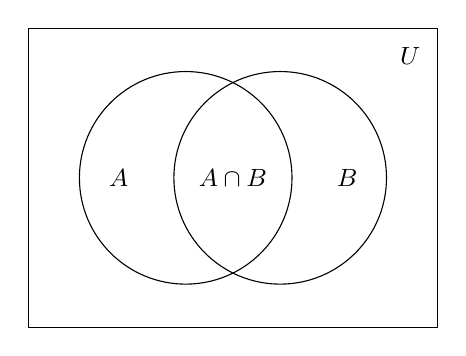
\begin{tikzpicture}
\draw (-2.6,-1.9) rectangle (2.6,1.9);
\node at (2.25,1.55) {$U$};
\draw (-0.6,0) circle (1.35);
\draw (0.6,0) circle (1.35);
\node at (-1.45,0) {$A$};
\node at (1.45,0) {$B$};
\node at (0,0) {$A\cap B$};
\end{tikzpicture}
\caption{Two sets. The whole shaded-looking region inside both circles is $A\cup B$; the overlap alone is $A\cap B$; everything outside both circles but inside the rectangle is $(A\cup B)^c$.}
\end{figure}

With three sets the picture has eight regions --- seven inside the circles and one
outside them all. Every element of $U$ lies in exactly one of them, which is what
makes the diagram useful for counting.

\begin{figure}[H]
\centering
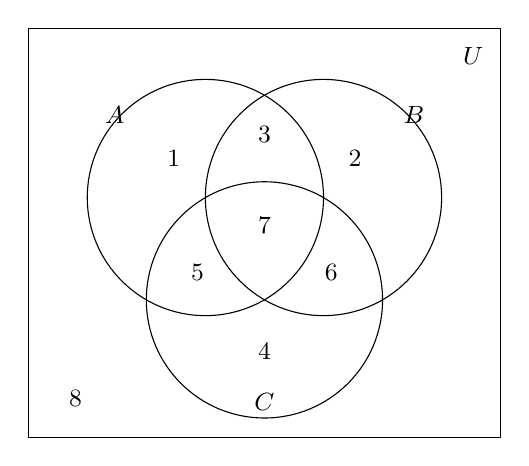
\begin{tikzpicture}
\draw (-3,-2.6) rectangle (3,2.6);
\node at (2.65,2.25) {$U$};
\draw (-0.75,0.45) circle (1.5);
\draw (0.75,0.45) circle (1.5);
\draw (0,-0.85) circle (1.5);
\node at (-1.9,1.5) {$A$};
\node at (1.9,1.5) {$B$};
\node at (0,-2.15) {$C$};
\node at (-1.15,0.95) {\small 1};
\node at (1.15,0.95) {\small 2};
\node at (0,1.25) {\small 3};
\node at (0,-1.5) {\small 4};
\node at (-0.85,-0.5) {\small 5};
\node at (0.85,-0.5) {\small 6};
\node at (0,0.1) {\small 7};
\node at (-2.4,-2.1) {\small 8};
\end{tikzpicture}
\caption{Three sets divide $U$ into eight regions: 7 is in all three, 3, 5 and 6 are in exactly two, 1, 2 and 4 are in exactly one, and 8 is in none.}
\end{figure}

\begin{example}
Let $U=\{a,b,c,d,e,f,g,h\}$, $A=\{a,c,g\}$, $B=\{b,c,f,g\}$ and $C=\{b,d,e,f,g\}$.
Find (a) $B\cup C$, (b) $A^c$, (c) $A^c\cap(B\cup C)$.
\end{example}

\begin{solution}
\textbf{(a)} Collect everything in either set:
$$B\cup C=\{b,c,d,e,f,g\}.$$

\textbf{(b)} Everything in $U$ but not in $A$:
$$A^c=\{b,d,e,f,h\}.$$

\textbf{(c)} Now intersect the two answers. Work through $A^c$ one element at a time
and keep those also in $B\cup C$: $b$ yes, $d$ yes, $e$ yes, $f$ yes, $h$ no.
$$A^c\cap(B\cup C)=\{b,d,e,f\}.$$
Notice the brackets were done first. Without them, $A^c\cap B\cup C$ would be
ambiguous.
\end{solution}

\subsubsection{Counting with a Venn diagram}

This is the application first-year students meet most often, and the one where a
diagram is not optional --- it is the method.

\begin{example}
A survey of $200$ students asked which of Economics, Statistics and Computing they
were taking. The results were:
\begin{table}[H]
\centering
\begin{tabular}{|l|c|}
\hline
Economics & 90\\
Statistics & 80\\
Computing & 70\\
Economics and Statistics & 35\\
Economics and Computing & 30\\
Statistics and Computing & 25\\
All three & 12\\
\hline
\end{tabular}
\end{table}
\begin{enumerate}
\item[(a).] Represent the information on a Venn diagram.
\item[(b).] How many students take none of the three?
\item[(c).] How many take exactly one?
\item[(d).] How many take exactly two?
\end{enumerate}
\end{example}

\begin{solution}
\textbf{The rule that makes this work: fill the diagram from the middle outwards.}
The figures such as ``$35$ take Economics and Statistics'' include the students who
take all three, so they cannot be written straight into the diagram. Start with the
centre, where the count is unambiguous, and subtract as you move out.

\textbf{Step 1 --- the centre.} All three: $12$.

\textbf{Step 2 --- exactly two.} Each pairwise figure includes the $12$ in the middle,
so remove them:
\begin{align*}
\text{Economics and Statistics only} &= 35-12 = 23\\
\text{Economics and Computing only} &= 30-12 = 18\\
\text{Statistics and Computing only} &= 25-12 = 13
\end{align*}

\textbf{Step 3 --- exactly one.} Each subject total includes everyone taking it,
so remove the three regions already filled inside that circle:
\begin{align*}
\text{Economics only} &= 90-23-18-12 = 37\\
\text{Statistics only} &= 80-23-13-12 = 32\\
\text{Computing only} &= 70-18-13-12 = 27
\end{align*}

\begin{figure}[H]
\centering
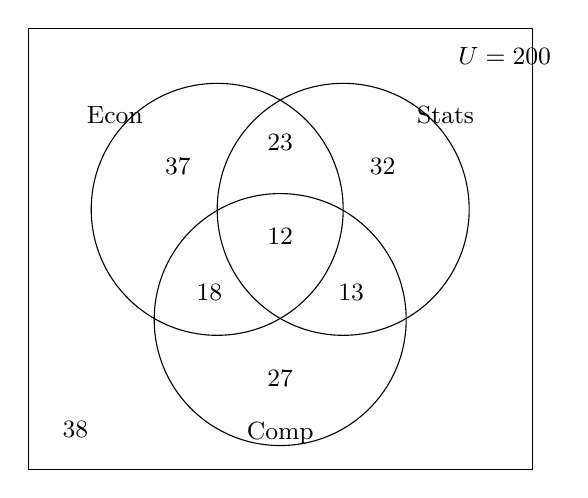
\begin{tikzpicture}
\draw (-3.2,-2.8) rectangle (3.2,2.8);
\node at (2.85,2.45) {$U=200$};
\draw (-0.8,0.5) circle (1.6);
\draw (0.8,0.5) circle (1.6);
\draw (0,-0.9) circle (1.6);
\node at (-2.1,1.7) {Econ};
\node at (2.1,1.7) {Stats};
\node at (0,-2.35) {Comp};
\node at (-1.3,1.05) {37};
\node at (1.3,1.05) {32};
\node at (0,1.35) {23};
\node at (0,-1.65) {27};
\node at (-0.9,-0.55) {18};
\node at (0.9,-0.55) {13};
\node at (0,0.15) {12};
\node at (-2.6,-2.3) {38};
\end{tikzpicture}
\caption{The completed diagram. Every one of the eight regions now holds a count, and they total 200.}
\end{figure}

\textbf{(b)} Add the seven regions inside the circles:
$$37+32+27+23+18+13+12=162,$$
so the number taking none is
$$200-162=38.$$

\textbf{(c)} Exactly one means the three outer regions:
$$37+32+27=96.$$

\textbf{(d)} Exactly two means the three overlap regions, not counting the centre:
$$23+18+13=54.$$

\textbf{Check.} The number taking at least one can also be found without the diagram,
by the \textbf{inclusion--exclusion principle}:
$$n(E\cup S\cup C)=n(E)+n(S)+n(C)-n(E\cap S)-n(E\cap C)-n(S\cap C)+n(E\cap S\cap C)$$
$$=90+80+70-35-30-25+12=162,$$
which agrees. Adding the three totals counts the pairwise overlaps twice, so they are
subtracted; but that removes the centre three times when it was added three times, so
it must be put back once. Getting $162$ by both routes is good evidence the diagram
was filled correctly.
\end{solution}

\begin{remark}
The commonest error in this kind of question is writing $35$ into the
Economics-and-Statistics region directly. Do that and every later figure is wrong,
and the eight regions will not total $200$ --- which is exactly why the total is worth
checking at the end.
\end{remark}

\subsection{Laws of the algebra of sets}

Set operations obey rules much like those of ordinary algebra. For any sets $A$, $B$,
$C$ in a universal set $U$:

\begin{table}[H]
\centering
\begin{tabular}{|l|l|l|}
\hline
Name & For $\cup$ & For $\cap$\\
\hline
Idempotent & $A\cup A=A$ & $A\cap A=A$\\
Commutative & $A\cup B=B\cup A$ & $A\cap B=B\cap A$\\
Associative & $(A\cup B)\cup C=A\cup(B\cup C)$ & $(A\cap B)\cap C=A\cap(B\cap C)$\\
Distributive & $A\cup(B\cap C)=(A\cup B)\cap(A\cup C)$ & $A\cap(B\cup C)=(A\cap B)\cup(A\cap C)$\\
Identity & $A\cup\varnothing=A$ & $A\cap U=A$\\
 & $A\cup U=U$ & $A\cap\varnothing=\varnothing$\\
Complement & $A\cup A^c=U$ & $A\cap A^c=\varnothing$\\
 & $(A^c)^c=A$ & $U^c=\varnothing,\ \varnothing^c=U$\\
De Morgan & $(A\cup B)^c=A^c\cap B^c$ & $(A\cap B)^c=A^c\cup B^c$\\
\hline
\end{tabular}
\caption{The laws of set algebra. Each column mirrors the other with $\cup$ and $\cap$ interchanged, and $\varnothing$ and $U$ interchanged.}
\end{table}

That mirroring is called \textbf{duality}, and it halves the number of laws worth
memorising: learn one column and swap the symbols to get the other.

\begin{note}
\textbf{De Morgan's laws in words.} ``Not (A or B)'' means ``not A and not B''; ``not
(A and B)'' means ``not A or not B''. Notice that the operation \emph{changes} when
the complement is taken through the bracket. Forgetting to change $\cup$ into $\cap$
is the usual slip.
\end{note}

\begin{example}
Verify De Morgan's law $(A\cup B)^c=A^c\cap B^c$ for
$$U=\{1,2,3,4,5,6,7,8\},\quad A=\{1,2,3,4\},\quad B=\{3,4,5,6\}.$$
\end{example}

\begin{solution}
Work out each side separately and compare.

\textbf{Left-hand side.}
$$A\cup B=\{1,2,3,4,5,6\}\quad\implies\quad (A\cup B)^c=\{7,8\}.$$

\textbf{Right-hand side.}
$$A^c=\{5,6,7,8\},\qquad B^c=\{1,2,7,8\}$$
$$\implies\quad A^c\cap B^c=\{7,8\}.$$

Both sides give $\{7,8\}$, so the law holds for these sets.
\end{solution}

\begin{remark}
Checking one example does not \emph{prove} a law --- it only fails to disprove it. A
proof would argue about an arbitrary element $x$: if $x\notin A\cup B$ then $x$ is in
neither $A$ nor $B$, so $x\in A^c$ and $x\in B^c$, hence $x\in A^c\cap B^c$; and the
same reasoning runs backwards. That argument covers every possible set at once, which
no amount of examples can do.
\end{remark}

\begin{example}
Simplify $\left(A^c\cup B\right)^c\cup\left(A\cap B\right)$.
\end{example}

\begin{solution}
Take the outer complement first, using De Morgan:
$$\left(A^c\cup B\right)^c=\left(A^c\right)^c\cap B^c=A\cap B^c.$$
So the expression becomes
$$\left(A\cap B^c\right)\cup\left(A\cap B\right).$$
Both terms contain $A$, so factor it out by the distributive law:
$$=A\cap\left(B^c\cup B\right)=A\cap U=A.$$

The whole expression collapses to $A$. Read on the diagram this is obvious: the first
part is everything in $A$ outside $B$, the second is everything in $A$ inside $B$, and
together they are all of $A$.
\end{solution}


\subsection{Practice problems}

Questions from Tutorial Sheet 1. Work each one before opening the solution.

\begin{problem}
Let $E$ be the universal set, $E=\{x: x\leq 13,\ x\in\mathbb{W}\}$, and let
$$A=\{1,2,3,4,5\},\quad B=\{4,5,6,7\},\quad C=\{5,6,7,8,9\},$$
$$D=\{x: 1<x<10,\ x=2k+1,\ k\in\mathbb{N}\},\quad
G=\{x: 1\leq x<13,\ x=2k,\ k\in\mathbb{N}\},\quad F=\{1,5,9\}.$$
\begin{enumerate}
\item[(i).] List the sets $E$, $D$ and $G$. Hence find
\item[(ii).] $A\cap\left(C\cup G^c\right)$
\item[(iii).] $A-B$
\item[(iv).] $(A\cap B)-C$
\item[(v).] $F-(A\cap D)^c$
\end{enumerate}
\end{problem}

\begin{solution}
\textbf{(i).} $\mathbb{W}$ is the set of whole numbers $\{0,1,2,\ldots\}$, so $E$ collects
the whole numbers up to and including $13$:
$$E=\{0,1,2,3,4,5,6,7,8,9,10,11,12,13\}.$$

For $D$, run through $k=1,2,3,\ldots$ and keep the values of $2k+1$ that fall strictly
between $1$ and $10$:
$$k=1\to 3,\quad k=2\to 5,\quad k=3\to 7,\quad k=4\to 9,\quad k=5\to 11\ (\text{too
big}).$$
$$D=\{3,5,7,9\}.$$

For $G$, keep the values of $2k$ with $1\leq 2k<13$:
$$k=1\to 2,\quad k=2\to 4,\quad \ldots,\quad k=6\to 12,\quad k=7\to 14\ (\text{too
big}).$$
$$G=\{2,4,6,8,10,12\}.$$

\textbf{(ii).} Work outwards from the innermost bracket. First the complement, taken
inside $E$:
$$G^c=E-G=\{0,1,3,5,7,9,11,13\}.$$
Then the union:
$$C\cup G^c=\{5,6,7,8,9\}\cup\{0,1,3,5,7,9,11,13\}=\{0,1,3,5,6,7,8,9,11,13\}.$$
Finally intersect with $A=\{1,2,3,4,5\}$, keeping only what appears in both:
$$A\cap\left(C\cup G^c\right)=\{1,3,5\}.$$

\textbf{(iii).} $A-B$ means the elements of $A$ that are not in $B$. From
$A=\{1,2,3,4,5\}$ remove $4$ and $5$:
$$A-B=\{1,2,3\}.$$

\textbf{(iv).} First $A\cap B=\{4,5\}$. Now remove anything also in $C=\{5,6,7,8,9\}$,
which removes the $5$:
$$(A\cap B)-C=\{4\}.$$

\textbf{(v).} First $A\cap D=\{1,2,3,4,5\}\cap\{3,5,7,9\}=\{3,5\}$, so
$$(A\cap D)^c=E-\{3,5\}=\{0,1,2,4,6,7,8,9,10,11,12,13\}.$$
Now take from $F=\{1,5,9\}$ the elements not in that set. Both $1$ and $9$ are in it, and
$5$ is not:
$$F-(A\cap D)^c=\{5\}.$$

\begin{note}
Part (v) is quicker with a small piece of algebra. Removing everything outside a set is
the same as keeping everything inside it:
$$F-X^c=F\cap X,$$
so $F-(A\cap D)^c=F\cap\{3,5\}=\{5\}$ in one line. Spotting this saves listing a
twelve-element complement.
\end{note}
\end{solution}

\begin{problem}
Let $E=\{x: x\in\mathbb{Z},\ 0\leq x\leq 21\}$ be the universal set,
$$A=\{x: x=2k-2,\ x<20,\ k\in\mathbb{N}\},\quad B=\{1,3,8,19,20\},\quad
C=\{1,2,6,8,9,11,15\}.$$
Draw a Venn diagram, and find
\begin{enumerate}
\item[(i).] $A^c\cap B^c$
\item[(ii).] $(A\cup B)\cap C$
\item[(iii).] $A-(B\cup C)$
\item[(iv).] $(A\cup B)^c$
\end{enumerate}
\end{problem}

\begin{solution}
\textbf{Listing $A$.} With $k=1,2,3,\ldots$ the values $2k-2$ are
$0,2,4,6,\ldots$, stopping before $20$:
$$A=\{0,2,4,6,8,10,12,14,16,18\},$$
the even numbers from $0$ to $18$. The universal set is
$E=\{0,1,2,\ldots,21\}$.

\textbf{The Venn diagram.} Placing each of the $22$ elements in exactly one region:

\begin{table}[H]
\centering
\begin{tabular}{|l|l|}
\hline
Region & Elements\\
\hline
$A$ only & $0,\ 4,\ 10,\ 12,\ 14,\ 16,\ 18$\\
$B$ only & $3,\ 19,\ 20$\\
$C$ only & $9,\ 11,\ 15$\\
$A\cap B$ only & --- \\
$A\cap C$ only & $2,\ 6$\\
$B\cap C$ only & $1$\\
$A\cap B\cap C$ & $8$\\
Outside all three & $5,\ 7,\ 13,\ 17,\ 21$\\
\hline
\end{tabular}
\end{table}

The eight counts are $7+3+3+0+2+1+1+5=22$, which is the size of $E$ --- the check that
nothing has been placed twice or left out.

\begin{figure}[H]
\centering
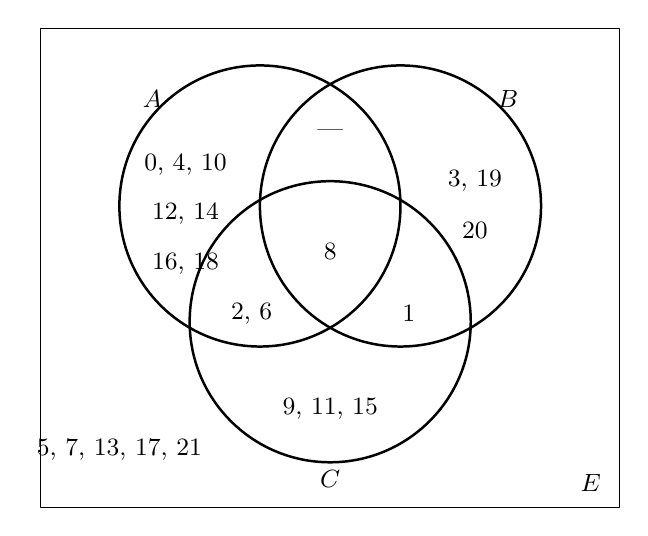
\begin{tikzpicture}[scale=1.05]
\draw (-3.5,-3.2) rectangle (3.5,2.6);
\node at (3.15,-2.9) {\small $E$};
\draw[thick] (-0.85,0.45) circle (1.7);
\draw[thick] (0.85,0.45) circle (1.7);
\draw[thick] (0,-0.95) circle (1.7);
\node at (-2.15,1.75) {\small $A$};
\node at (2.15,1.75) {\small $B$};
\node at (0,-2.85) {\small $C$};
% A only
\node[font=\small] at (-1.75,0.95) {$0,\,4,\,10$};
\node[font=\small] at (-1.75,0.35) {$12,\,14$};
\node[font=\small] at (-1.75,-0.25) {$16,\,18$};
% B only
\node[font=\small] at (1.75,0.75) {$3,\,19$};
\node[font=\small] at (1.75,0.15) {$20$};
% C only
\node[font=\small] at (0,-2.0) {$9,\,11,\,15$};
% A n B only  (empty)
\node[font=\small] at (0,1.35) {---};
% A n C only
\node[font=\small] at (-0.95,-0.85) {$2,\,6$};
% B n C only
\node[font=\small] at (0.95,-0.85) {$1$};
% centre
\node[font=\small] at (0,-0.1) {$8$};
% outside
\node[font=\small] at (-2.55,-2.5) {$5,\,7,\,13,\,17,\,21$};
\end{tikzpicture}
\caption{The 22 elements of $E$ placed in the eight regions. $A\cap B$ has nothing in it except the centre, so the region for $A$ and $B$ alone is empty; the five elements outside every circle are the ones counted by $(A\cup B)^c$ in part (i).}
\end{figure}


\textbf{(i).} $A^c$ is everything in $E$ outside $A$, and $B^c$ everything outside $B$.
Their intersection is what lies outside \emph{both}:
$$A\cup B=\{0,1,2,3,4,6,8,10,12,14,16,18,19,20\},$$
$$A^c\cap B^c=E-(A\cup B)=\{5,7,9,11,13,15,17,21\}.$$

\textbf{(ii).} $(A\cup B)\cap C$ keeps the elements of $C$ that appear in $A$ or in $B$.
Testing each element of $C=\{1,2,6,8,9,11,15\}$ in turn: $1\in B$, $2\in A$, $6\in A$,
$8\in A$, while $9$, $11$ and $15$ are in neither.
$$(A\cup B)\cap C=\{1,2,6,8\}.$$

\textbf{(iii).} $B\cup C=\{1,2,3,6,8,9,11,15,19,20\}$. Removing these from $A$:
$$A-(B\cup C)=\{0,4,10,12,14,16,18\}.$$

\textbf{(iv).} $(A\cup B)^c=E-(A\cup B)=\{5,7,9,11,13,15,17,21\}.$

\begin{note}
Parts (i) and (iv) give the same answer, and that is not a coincidence. It is De
Morgan's law,
$$A^c\cap B^c=(A\cup B)^c,$$
appearing in a concrete case. Whenever two parts of a question produce the same set, look
for the law that made it happen.
\end{note}
\end{solution}

\begin{problem}
Find the power set of each of the following.
\begin{enumerate}
\item[(i).] $A=\{\ \}$
\item[(ii).] $B=\{1,2\}$
\item[(iii).] $V=\{x: x \text{ is a vowel of the English alphabet}\}$
\end{enumerate}
\end{problem}

\begin{solution}
The power set $P(S)$ is the set of \emph{all} subsets of $S$, and it always contains
both $\emptyset$ and $S$ itself.

\textbf{(i).} The empty set has exactly one subset --- itself. So
$$P(A)=\{\emptyset\},$$
a set with one element. Note that $P(A)$ is \emph{not} empty: it is a box containing an
empty box.

\textbf{(ii).} List the subsets by size --- none, one element, then two:
$$P(B)=\Big\{\ \emptyset,\ \{1\},\ \{2\},\ \{1,2\}\ \Big\},$$
which has $4$ elements.

\textbf{(iii).} $V=\{a,e,i,o,u\}$, with $n(V)=5$, so
$$n\left(P(V)\right)=2^5=32.$$
Grouped by size, the $32$ subsets are:

\begin{table}[H]
\centering
\begin{tabular}{|l|c|l|}
\hline
Size & How many & Subsets\\
\hline
0 & 1 & $\emptyset$\\
1 & 5 & $\{a\},\{e\},\{i\},\{o\},\{u\}$\\
2 & 10 & $\{a,e\},\{a,i\},\{a,o\},\{a,u\},\{e,i\},\{e,o\},\{e,u\},\{i,o\},\{i,u\},\{o,u\}$\\
3 & 10 & $\{a,e,i\},\{a,e,o\},\{a,e,u\},\{a,i,o\},\{a,i,u\},\{a,o,u\},$\\
  &    & $\{e,i,o\},\{e,i,u\},\{e,o,u\},\{i,o,u\}$\\
4 & 5 & $\{e,i,o,u\},\{a,i,o,u\},\{a,e,o,u\},\{a,e,i,u\},\{a,e,i,o\}$\\
5 & 1 & $\{a,e,i,o,u\}$\\
\hline
\multicolumn{2}{|l|}{\textbf{Total}} & $1+5+10+10+5+1=32$\ \checkmark\\
\hline
\end{tabular}
\end{table}

\begin{note}
A set with $n$ elements has $2^n$ subsets, because each element is independently either
in a given subset or out of it --- two choices, $n$ times over. Checking the count
against $2^n$ before writing the list out is the only reliable way to know none have been
missed.
\end{note}
\end{solution}

\begin{problem}
\begin{enumerate}
\item[(a).] If $A\subset B$, simplify \quad (i) $(A\cap B)^c$, \quad (ii) $A\cup B^c$,
\quad (iii) $\left(B\cap A^c\right)\cup A$.
\item[(b).] If $A$ and $B$ are disjoint subsets of the universal set $E$, simplify
\quad (i) $A\cap B$, \quad (ii) $A\cap B^c$, \quad (iii) $A^c\cup B^c$.
\end{enumerate}
\end{problem}

\begin{solution}
\textbf{(a)} $A\subset B$ means every element of $A$ is also in $B$: the circle for $A$
sits entirely inside the circle for $B$.

\textbf{(i).} Since all of $A$ lies in $B$, the overlap is the whole of $A$:
$$A\cap B=A\quad\implies\quad (A\cap B)^c=A^c.$$

\textbf{(ii).} $A\cup B^c$ is everything that is in $A$ or outside $B$. What is missing
is exactly what is in $B$ but not in $A$, so
$$A\cup B^c=(B-A)^c.$$
Checking with De Morgan: $(B-A)^c=\left(B\cap A^c\right)^c=B^c\cup A$, which is the same
set.

\textbf{(iii).} $B\cap A^c$ is the part of $B$ outside $A$, namely $B-A$. Adding $A$
back restores the whole of $B$:
$$\left(B\cap A^c\right)\cup A=(B-A)\cup A=B.$$

\textbf{(b)} Disjoint means the two circles do not touch: $A\cap B=\emptyset$.

\textbf{(i).} That is the definition itself:
$$A\cap B=\emptyset.$$

\textbf{(ii).} $A\cap B^c$ is the part of $A$ lying outside $B$. Since none of $A$ is
inside $B$, that is all of it:
$$A\cap B^c=A.$$

\textbf{(iii).} By De Morgan and part (i):
$$A^c\cup B^c=(A\cap B)^c=\emptyset^c=E.$$
\end{solution}

\begin{problem}
Express each of the following in its simplest form.
\begin{enumerate}
\item[(i).] $(A\cup B)\cap\left(A\cup B^c\right)$
\item[(ii).] $\left[(X\cap Y)^c\cup(X-Y)\right]^c$
\item[(iii).] $B^c\cap(A\cup B)$
\item[(iv).] $\left[A^c\cup\left(A\cap B^c\right)\right]^c$
\end{enumerate}
\end{problem}

\begin{solution}
\textbf{(i).} The distributive law lets $A$ be taken outside:
$$(A\cup B)\cap\left(A\cup B^c\right)=A\cup\left(B\cap B^c\right)=A\cup\emptyset=A.$$

\textbf{(ii).} Apply De Morgan to the outer complement first:
$$\left[(X\cap Y)^c\cup(X-Y)\right]^c=(X\cap Y)\cap(X-Y)^c.$$
Now $X-Y=X\cap Y^c$, so by De Morgan again $(X-Y)^c=X^c\cup Y$. Hence
$$=(X\cap Y)\cap\left(X^c\cup Y\right)
=\left[(X\cap Y)\cap X^c\right]\cup\left[(X\cap Y)\cap Y\right].$$
The first bracket is empty, because nothing can be in $X$ and in $X^c$ at once. The
second is $X\cap Y$, because $X\cap Y$ is already inside $Y$. So
$$=\emptyset\cup(X\cap Y)=X\cap Y.$$

\textbf{(iii).} Distribute $B^c$ across the union:
$$B^c\cap(A\cup B)=\left(B^c\cap A\right)\cup\left(B^c\cap B\right)
=\left(A\cap B^c\right)\cup\emptyset=A-B.$$

\textbf{(iv).} De Morgan on the outer complement:
$$\left[A^c\cup\left(A\cap B^c\right)\right]^c=A\cap\left(A\cap B^c\right)^c
=A\cap\left(A^c\cup B\right).$$
Distributing:
$$=\left(A\cap A^c\right)\cup(A\cap B)=\emptyset\cup(A\cap B)=A\cap B.$$

\begin{note}
The pattern in (ii) and (iv) is the same: when a complement sits outside a large
bracket, use De Morgan to push it inwards first, and only then distribute. Trying to
simplify inside the bracket before dealing with the outer complement leads to much
longer expressions.
\end{note}
\end{solution}

\begin{problem}
In each of the Venn diagrams below, shade the region representing
\quad (i) $B\cap(A-C)^c$, \quad (ii) $B\cap(A\cup C)^c$.
\end{problem}

\begin{solution}
\textbf{(i).} Reading the expression: take $B$, and remove from it everything that lies
in $A$ but not in $C$. The set $A-C$ is the part of $A$ outside $C$; intersecting $B$
with its complement keeps the rest of $B$.

Of the four regions making up $B$, only one --- the part in $A$ but not in $C$ --- is in
$A-C$. So the shading is all of $B$ except that piece: $B$ alone, $B\cap C$ alone, and
the centre $A\cap B\cap C$.

\begin{figure}[H]
\centering
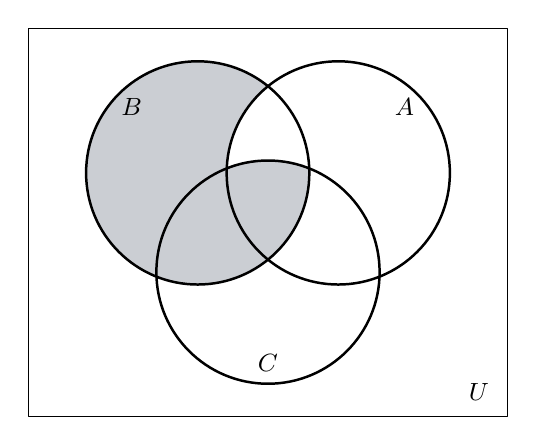
\begin{tikzpicture}[scale=1.05]
\draw (-2.9,-2.5) rectangle (2.9,2.2);
\node at (2.55,-2.2) {\small $U$};
\begin{scope}
  \clip (-0.85,0.45) circle (1.35);
  \fill[gray!35] (-3,-2.6) rectangle (3,2.3);
  \begin{scope}
    \clip (0.85,0.45) circle (1.35);
    \fill[white] (-3,-2.6) rectangle (3,2.3);
  \end{scope}
\end{scope}
\begin{scope}
  \clip (-0.85,0.45) circle (1.35);
  \clip (0.85,0.45) circle (1.35);
  \clip (0,-0.75) circle (1.35);
  \fill[gray!35] (-3,-2.6) rectangle (3,2.3);
\end{scope}
\draw[thick] (-0.85,0.45) circle (1.35);
\draw[thick] (0.85,0.45) circle (1.35);
\draw[thick] (0,-0.75) circle (1.35);
\node at (-1.65,1.25) {\small $B$};
\node at (1.65,1.25) {\small $A$};
\node at (0,-1.85) {\small $C$};
\end{tikzpicture}
\caption{$B\cap(A-C)^c$: all of $B$ except the part lying in $A$ but outside $C$.}
\end{figure}

\textbf{(ii).} Here $C$ lies wholly inside $B$, and $A$ overlaps both. The expression
takes $B$ and removes everything belonging to $A$ or to $C$, so what is left is the part
of $B$ lying outside both circles.

\begin{figure}[H]
\centering
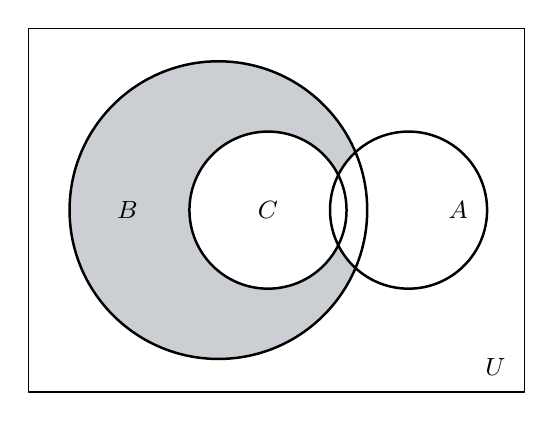
\begin{tikzpicture}[scale=1.05]
\draw (-2.9,-2.2) rectangle (3.1,2.2);
\node at (2.75,-1.9) {\small $U$};
\begin{scope}
  \clip (-0.6,0) circle (1.8);
  \fill[gray!35] (-3,-2.3) rectangle (3.2,2.3);
  \begin{scope}
    \clip (1.7,0) circle (0.95);
    \fill[white] (-3,-2.3) rectangle (3.2,2.3);
  \end{scope}
  \begin{scope}
    \clip (0,0) circle (0.95);
    \fill[white] (-3,-2.3) rectangle (3.2,2.3);
  \end{scope}
\end{scope}
\draw[thick] (-0.6,0) circle (1.8);
\draw[thick] (0,0) circle (0.95);
\draw[thick] (1.7,0) circle (0.95);
\node at (-1.7,0) {\small $B$};
\node at (0,0) {\small $C$};
\node at (2.3,0) {\small $A$};
\end{tikzpicture}
\caption{$B\cap(A\cup C)^c$: the part of $B$ outside both $A$ and $C$.}
\end{figure}

\begin{note}
In both parts the complement is the piece to read carefully. $(A-C)^c$ and $(A\cup C)^c$
are each enormous regions stretching outside all the circles, but intersecting with $B$
confines the answer to inside $B$. Shade $B$ first and then rub out, rather than trying
to shade the complement itself.
\end{note}
\end{solution}

\begin{problem}
People consume tobacco by three methods: smoking (SM), sniffing (SN) or chewing (CH). A
survey of $70$ tobacco consumers found that $56$ smoked, $56$ sniffed and $50$ chewed;
$48$ both smoked and sniffed, $42$ both smoked and chewed, and $44$ both sniffed and
chewed. Determine the number who used all three methods.
\end{problem}

\begin{solution}
\textbf{Step 1 --- write down what is known.} Every one of the $70$ uses at least one
method, so
$$n(\text{SM}\cup\text{SN}\cup\text{CH})=70,$$
$$n(\text{SM})=56,\quad n(\text{SN})=56,\quad n(\text{CH})=50,$$
$$n(\text{SM}\cap\text{SN})=48,\quad n(\text{SM}\cap\text{CH})=42,\quad
n(\text{SN}\cap\text{CH})=44.$$

\textbf{Step 2 --- use the inclusion--exclusion rule for three sets.} Writing $x$ for
the number using all three,
$$n(\text{SM}\cup\text{SN}\cup\text{CH})=n(\text{SM})+n(\text{SN})+n(\text{CH})
-n(\text{SM}\cap\text{SN})-n(\text{SM}\cap\text{CH})-n(\text{SN}\cap\text{CH})+x.$$

\textbf{Step 3 --- substitute and solve.}
$$70=56+56+50-48-42-44+x$$
$$70=162-134+x=28+x$$
$$\implies\quad x=42.$$

$$\therefore\quad 42 \text{ people used all three methods}.$$

\textbf{Step 4 --- check by filling in every region.} Working from the centre outwards:

\begin{table}[H]
\centering
\begin{tabular}{|l|l|c|}
\hline
Region & Calculation & Number\\
\hline
All three & given by Step 3 & 42\\
SM and SN only & $48-42$ & 6\\
SM and CH only & $42-42$ & 0\\
SN and CH only & $44-42$ & 2\\
SM only & $56-6-0-42$ & 8\\
SN only & $56-6-2-42$ & 6\\
CH only & $50-0-2-42$ & 6\\
\hline
\textbf{Total} & $42+6+0+2+8+6+6$ & \textbf{70}\ \checkmark\\
\hline
\end{tabular}
\end{table}

\begin{note}
Every region comes out zero or positive and the total is exactly $70$, so the answer is
consistent. Had any region come out negative, the data itself would have been
contradictory --- and that check is worth doing, because it costs a minute and catches
both arithmetic slips and impossible questions.
\end{note}
\end{solution}

\begin{problem}
In a class of $100$ students, $60$ like Mathematics, $40$ like Economics and $45$ like
Demography. In addition, $20$ like both Mathematics and Economics, $25$ like both
Economics and Demography, $30$ like both Mathematics and Demography, and $15$ like all
three.
\begin{enumerate}
\item[(a).] Draw a Venn diagram to represent this information.
\item[(b).] Find the number of students who like exactly one course.
\item[(c).] Find the number who like neither Economics nor Demography.
\end{enumerate}
\end{problem}

\begin{solution}
Write $M$, $E$ and $D$ for the three sets.

\textbf{(a).} Always start at the centre and work outwards, subtracting what has already
been placed.

\begin{table}[H]
\centering
\begin{tabular}{|l|l|c|}
\hline
Region & Calculation & Number\\
\hline
$M\cap E\cap D$ & given & 15\\
$M\cap E$ only & $20-15$ & 5\\
$E\cap D$ only & $25-15$ & 10\\
$M\cap D$ only & $30-15$ & 15\\
$M$ only & $60-5-15-15$ & 25\\
$E$ only & $40-5-10-15$ & 10\\
$D$ only & $45-10-15-15$ & 5\\
Outside all three & $100-85$ & 15\\
\hline
\textbf{Total} & & \textbf{100}\ \checkmark\\
\hline
\end{tabular}
\end{table}

\begin{figure}[H]
\centering
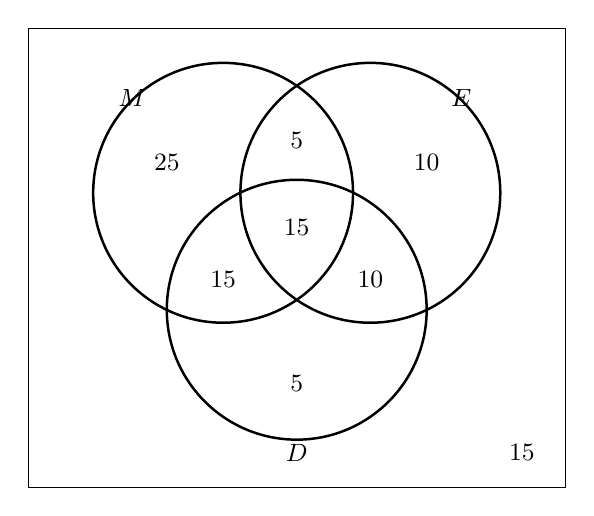
\begin{tikzpicture}[scale=1.1]
\draw (-3.1,-2.9) rectangle (3.1,2.4);
\draw[thick] (-0.85,0.5) circle (1.5);
\draw[thick] (0.85,0.5) circle (1.5);
\draw[thick] (0,-0.85) circle (1.5);
\node at (-1.9,1.6) {\small $M$};
\node at (1.9,1.6) {\small $E$};
\node at (0,-2.5) {\small $D$};
\node at (-1.5,0.85) {\small 25};
\node at (1.5,0.85) {\small 10};
\node at (0,-1.7) {\small 5};
\node at (0,1.1) {\small 5};
\node at (-0.85,-0.5) {\small 15};
\node at (0.85,-0.5) {\small 10};
\node at (0,0.1) {\small 15};
\node at (2.6,-2.5) {\small 15};
\end{tikzpicture}
\caption{The 100 students. The eight regions sum to 100, which is the check that the diagram is right.}
\end{figure}

\textbf{(b).} ``Exactly one'' means the three outer regions only:
$$25+10+5=40.$$

$$\therefore\quad 40 \text{ students like exactly one course}.$$

\textbf{(c).} ``Neither Economics nor Demography'' is $(E\cup D)^c$. First
$$n(E\cup D)=n(E)+n(D)-n(E\cap D)=40+45-25=60,$$
so
$$n\left((E\cup D)^c\right)=100-60=40.$$

$$\therefore\quad 40 \text{ students like neither Economics nor Demography}.$$

\begin{note}
The answer to (c) can be read straight off the diagram as a check: the students outside
both $E$ and $D$ are the $25$ who like Mathematics only together with the $15$ who like
none, giving $25+15=40$. Two independent routes to the same number is worth more than
one route done carefully.
\end{note}

\begin{note}
Parts (b) and (c) happen to give the same number, $40$. They are different sets of
students --- (b) counts $25+10+5$ and (c) counts $25+15$ --- and the coincidence means
nothing. Do not let a repeated answer persuade you that two questions were the same
question.
\end{note}
\end{solution}

\begin{problem}
A survey of $80$ snack consumers found that $62$ eat chips (CH), $55$ drink soda (SO)
and $48$ eat candy (CA). In addition, $40$ eat chips and drink soda, $35$ eat chips and
candy, and $42$ drink soda and eat candy. Find
\begin{enumerate}
\item[(a).] the number of customers who take all three;
\item[(b).] the number taking exactly two snacks.
\end{enumerate}
\end{problem}

\begin{solution}
\textbf{(a).} With $x$ the number taking all three, inclusion--exclusion gives
$$80=62+55+48-40-35-42+x$$
$$80=165-117+x=48+x$$
$$\implies\quad x=32.$$

$$\therefore\quad 32 \text{ customers take all three}.$$

\textbf{(b).} ``Exactly two'' excludes those taking all three, so each pairwise overlap
must have the $32$ removed from it:
$$\text{chips and soda only}=40-32=8,$$
$$\text{chips and candy only}=35-32=3,$$
$$\text{soda and candy only}=42-32=10,$$
$$\text{total}=8+3+10=21.$$

$$\therefore\quad 21 \text{ customers take exactly two snacks}.$$

\textbf{Check.} The single-snack regions are
$$62-40-35+32=19,\qquad 55-40-42+32=5,\qquad 48-35-42+32=3,$$
and the eight regions total
$$19+5+3+8+3+10+32=80.\ \checkmark$$

\begin{note}
The commonest error in (b) is to answer $40+35+42=117$, or to answer
$117-32=85$. Both are far larger than the $80$ people surveyed, which is why the
running total is worth glancing at. Each pairwise figure such as ``$40$ eat chips and
drink soda'' includes the $32$ who take all three, and it must be subtracted from each of
the three overlaps separately.
\end{note}
\end{solution}

\section{Sets of Numbers}

Numbers arrive in stages, and each stage exists because the one before it could not
do something. Counting needs the natural numbers; recording nothing needs zero;
owing needs the negatives; sharing needs fractions; measuring a diagonal needs
something none of those provide. This chapter names each set and the notation that
goes with it.

\subsection{From counting numbers to real numbers}

\begin{definition}
The \textbf{natural numbers} are the counting numbers,
$$\mathbb{N}=\{1,2,3,4,\ldots\}.$$
Including zero gives the \textbf{whole numbers},
$$W=\{0,1,2,3,4,\ldots\},$$
and including the negatives gives the \textbf{integers},
$$\mathbb{Z}=\{\ldots,-3,-2,-1,0,1,2,3,\ldots\}.$$
\end{definition}

\begin{figure}[H]
\centering
\begin{tikzpicture}
\draw[-Stealth](-4.2,0)--(4.2,0);
\foreach \x in {-3,-2,-1,0,1,2,3}{\draw(\x,-0.12)--(\x,0.12); \node at (\x,-0.45){\small $\x$};}
\end{tikzpicture}
\caption{The integers on a number line. Each is a whole step from the next.}
\end{figure}

Each set contains the one before it:
$$\mathbb{N}\subset W\subset\mathbb{Z}.$$

Dividing one integer by another does not usually give an integer, and that is what the
next set is for.

\begin{definition}
A \textbf{rational number} is any number that can be written as a fraction of two
integers with non-zero denominator:
$$\mathbb{Q}=\left\{\frac{p}{q} : p,q\in\mathbb{Z},\ q\neq 0\right\}.$$
\end{definition}

Every integer is rational, since $-3=\frac{-3}{1}$. So the chain extends:
$$\mathbb{N}\subset W\subset\mathbb{Z}\subset\mathbb{Q}.$$

\begin{remark}
In decimal form a rational number always does one of two things:
\begin{enumerate}
\item[(i).] it \textbf{terminates}, as $\frac{3}{4}=0.75$; or
\item[(ii).] it \textbf{recurs}, as $\frac{23}{11}=2.090909\ldots=2.\overline{09}$,
where the bar marks the block that repeats forever.
\end{enumerate}
Nothing else can happen. A decimal that neither stops nor settles into a repeating
block is not rational.
\end{remark}

That last sentence works in reverse too, and gives a method: any recurring decimal
can be turned back into a fraction.

\begin{example}
Express each recurring decimal as a fraction in its lowest terms.
\begin{enumerate}
\item[(a).] $0.\overline{45}$
\item[(b).] $2.\overline{3}$
\item[(c).] $0.1\overline{6}$
\end{enumerate}
\end{example}

\begin{solution}
The trick in every case is to multiply by a power of $10$ chosen so that the
recurring parts line up, then subtract to cancel them.

\textbf{(a)} The block $45$ has \emph{two} digits, so multiply by $10^2=100$.
\begin{align*}
\text{Let}\quad x &= 0.454545\ldots\\
100x &= 45.454545\ldots
\end{align*}
Subtracting the first line from the second, the endless tails cancel exactly:
$$100x-x=45.454545\ldots-0.454545\ldots=45$$
$$\implies\quad 99x=45\quad\implies\quad x=\frac{45}{99}=\frac{5}{11}.$$

\textbf{(b)} One recurring digit, so multiply by $10$.
\begin{align*}
\text{Let}\quad x &= 2.3333\ldots\\
10x &= 23.3333\ldots
\end{align*}
$$10x-x=21\quad\implies\quad 9x=21\quad\implies\quad x=\frac{21}{9}=\frac{7}{3}.$$

\textbf{(c)} Here the $1$ does not recur but the $6$ does, so \emph{two} multiplications
are needed --- one to step past the non-recurring digit, one to span the block.
\begin{align*}
\text{Let}\quad x &= 0.16666\ldots\\
10x &= 1.6666\ldots\\
100x &= 16.6666\ldots
\end{align*}
Now subtract the second from the third, since those two have matching tails:
$$100x-10x=15\quad\implies\quad 90x=15\quad\implies\quad x=\frac{15}{90}=\frac{1}{6}.$$

\textbf{Check.} $1\div 6=0.1666\ldots$, as required.
\end{solution}

\begin{note}
Subtract the two lines whose \emph{tails match}. In part (c), subtracting $x$ from
$100x$ would not work, because $0.1666\ldots$ and $16.6666\ldots$ do not have the same
digits after the point.
\end{note}

\begin{definition}
The \textbf{real numbers} $\mathbb{R}$ are all the numbers that correspond to points on
a number line. A real number that cannot be written as a fraction of integers is
called \textbf{irrational}.
\end{definition}

Examples of irrational numbers are $\sqrt{2}=1.41421\ldots$, $\sqrt{5}$ and
$\pi=3.14159\ldots$ Their decimals run forever without ever settling into a repeating
block. Together,
$$\mathbb{N}\subset W\subset\mathbb{Z}\subset\mathbb{Q}\subset\mathbb{R},$$
and the irrationals are exactly what is left of $\mathbb{R}$ after $\mathbb{Q}$ is
removed.

\subsection{Interval notation}

A set of real numbers between two endpoints is written as an \textbf{interval}. The
only thing to keep track of is whether the endpoints themselves are included.

\begin{table}[H]
\centering
\begin{tabular}{|l|l|l|}
\hline
Interval & Meaning & In set-builder notation\\
\hline
$[a,b]$ & closed: both ends included & $\{x\in\mathbb{R} : a\leq x\leq b\}$\\
$(a,b)$ & open: neither end included & $\{x\in\mathbb{R} : a< x< b\}$\\
$[a,b)$ & half-open & $\{x\in\mathbb{R} : a\leq x< b\}$\\
$(a,b]$ & half-open & $\{x\in\mathbb{R} : a< x\leq b\}$\\
$[a,\infty)$ & unbounded above & $\{x\in\mathbb{R} : x\geq a\}$\\
$(-\infty,b)$ & unbounded below & $\{x\in\mathbb{R} : x< b\}$\\
\hline
\end{tabular}
\caption{Interval notation. A square bracket includes the endpoint, a round one excludes it.}
\end{table}

\begin{note}
$\infty$ is not a number and can never be included, so it always takes a round
bracket: $[2,\infty)$, never $[2,\infty]$.
\end{note}

\begin{example}
Write each of the following in interval notation.
\begin{enumerate}
\item[(a).] All real numbers from $-1$ up to and including $4$.
\item[(b).] $\{x\in\mathbb{R} : x>7\}$
\item[(c).] All real numbers at most $0$ or at least $3$.
\end{enumerate}
\end{example}

\begin{solution}
\textbf{(a)} $-1$ is excluded by ``from'', $4$ is included by ``and including'':
$[-1,4]$ if $-1$ is meant to be included, and here ``from $-1$'' does include it, so
$$[-1,4].$$

\textbf{(b)} Strictly greater, so the endpoint is out and there is no upper limit:
$$(7,\infty).$$

\textbf{(c)} This is two separate pieces, joined by ``or'' --- a union:
$$(-\infty,0]\cup[3,\infty).$$
\end{solution}

\subsection{Radicals and rational powers}

\begin{definition}
If $a\geq 0$, the \textbf{square root} $\sqrt{a}$ is the non-negative number whose
square is $a$. More generally $a^{1/n}=\sqrt[n]{a}$ and
$a^{m/n}=\sqrt[n]{a^m}=\left(\sqrt[n]{a}\right)^m$.
\end{definition}

The rules that make radicals manageable are
$$\sqrt{ab}=\sqrt{a}\,\sqrt{b},\qquad \sqrt{\frac{a}{b}}=\frac{\sqrt{a}}{\sqrt{b}}
\quad (b\neq 0).$$

\begin{note}
There is no such rule for sums. $\sqrt{a+b}$ is \textbf{not} $\sqrt{a}+\sqrt{b}$. Test
it once and remember it: $\sqrt{9+16}=\sqrt{25}=5$, while $\sqrt{9}+\sqrt{16}=3+4=7$.
\end{note}

\subsubsection{Rationalising the denominator}

A fraction with a radical underneath is awkward to work with and, by convention, is
not left in that form. \textbf{Rationalising} means rewriting it so the denominator is
rational.

\begin{example}
Rationalise the denominator of each.
\begin{enumerate}
\item[(a).] $\frac{3}{\sqrt{5}}$
\item[(b).] $\frac{2}{\sqrt{7}-\sqrt{3}}$
\item[(c).] $\frac{1+\sqrt{2}}{3-\sqrt{2}}$
\end{enumerate}
\end{example}

\begin{solution}
\textbf{(a)} A single radical: multiply top and bottom by it.
$$\frac{3}{\sqrt{5}}=\frac{3}{\sqrt{5}}\times\frac{\sqrt{5}}{\sqrt{5}}
=\frac{3\sqrt{5}}{5}.$$
Multiplying by $\frac{\sqrt5}{\sqrt5}$ is multiplying by $1$, so the value has not
changed --- only its appearance.

\textbf{(b)} Two terms underneath. Multiply by the \textbf{conjugate}, the same
expression with the sign between the terms reversed, because
$(x-y)(x+y)=x^2-y^2$ removes both radicals at once.
$$\frac{2}{\sqrt{7}-\sqrt{3}}\times\frac{\sqrt{7}+\sqrt{3}}{\sqrt{7}+\sqrt{3}}
=\frac{2\left(\sqrt{7}+\sqrt{3}\right)}{\left(\sqrt{7}\right)^2-\left(\sqrt{3}\right)^2}
=\frac{2\left(\sqrt{7}+\sqrt{3}\right)}{7-3}
=\frac{2\left(\sqrt{7}+\sqrt{3}\right)}{4}
=\frac{\sqrt{7}+\sqrt{3}}{2}.$$

\textbf{(c)} Same method; the conjugate of $3-\sqrt{2}$ is $3+\sqrt{2}$.
$$\frac{1+\sqrt{2}}{3-\sqrt{2}}\times\frac{3+\sqrt{2}}{3+\sqrt{2}}
=\frac{\left(1+\sqrt{2}\right)\left(3+\sqrt{2}\right)}{9-2}.$$
Expanding the top:
$$\left(1+\sqrt{2}\right)\left(3+\sqrt{2}\right)
=3+\sqrt{2}+3\sqrt{2}+\left(\sqrt{2}\right)^2
=3+4\sqrt{2}+2=5+4\sqrt{2}.$$
$$\therefore\quad \frac{1+\sqrt{2}}{3-\sqrt{2}}=\frac{5+4\sqrt{2}}{7}.$$

\textbf{Check.} $\frac{1+\sqrt2}{3-\sqrt2}\approx 1.5224$ and
$\frac{5+4\sqrt2}{7}\approx 1.5224$. A quick numerical check like this catches sign
errors in the expansion, and takes seconds.
\end{solution}

\subsection{Complex numbers}

No real number squares to give a negative, so $x^2=-1$ has no real solution. Rather
than stop there, we give that missing number a name.

\begin{definition}
The \textbf{imaginary unit} $i$ is defined by
$$i^2=-1,\qquad\text{that is}\qquad i=\sqrt{-1}.$$
A \textbf{complex number} has the form $z=a+bi$ with $a,b\in\mathbb{R}$. Here $a$ is
the \textbf{real part} and $b$ the \textbf{imaginary part}, written
$\operatorname{Re}(z)=a$ and $\operatorname{Im}(z)=b$.
\end{definition}

\begin{note}
The imaginary part is the real number $b$, not $bi$. For $z=3+4i$,
$\operatorname{Im}(z)=4$.
\end{note}

Two complex numbers are \textbf{equal} exactly when their real parts match and their
imaginary parts match. That single fact turns one complex equation into two real ones,
which is how such equations are usually solved.

\subsubsection{Arithmetic with complex numbers}

Addition and subtraction are done part by part. Multiplication is ordinary expansion,
followed by replacing $i^2$ with $-1$.

\begin{example}
Let $z_1=3+4i$ and $z_2=1-2i$. Find (a) $z_1+z_2$, (b) $z_1-z_2$, (c) $z_1z_2$.
\end{example}

\begin{solution}
\textbf{(a)} Add real to real, imaginary to imaginary:
$$z_1+z_2=(3+1)+(4-2)i=4+2i.$$

\textbf{(b)} $$z_1-z_2=(3-1)+(4-(-2))i=2+6i.$$

\textbf{(c)} Expand as usual:
\begin{align*}
z_1z_2 &=(3+4i)(1-2i)\\
       &=3-6i+4i-8i^2\\
       &=3-2i-8i^2.
\end{align*}
Now use $i^2=-1$, so $-8i^2=-8(-1)=+8$:
$$z_1z_2=3+8-2i=11-2i.$$
\end{solution}

\begin{definition}
The \textbf{conjugate} of $z=a+bi$ is $\bar{z}=a-bi$: the same number with the sign of
the imaginary part reversed.
\end{definition}

The conjugate matters because a number times its conjugate is always real:
$$(a+bi)(a-bi)=a^2-(bi)^2=a^2-b^2i^2=a^2+b^2.$$
That is exactly the tool needed for division --- the same idea as rationalising a
denominator.

\begin{example}
Express $\frac{3+4i}{1-2i}$ in the form $a+bi$.
\end{example}

\begin{solution}
Multiply top and bottom by the conjugate of the denominator, $1+2i$:
$$\frac{3+4i}{1-2i}\times\frac{1+2i}{1+2i}=\frac{(3+4i)(1+2i)}{1^2+2^2}.$$

The denominator is now real: $1^2+2^2=5$. Expanding the numerator,
$$(3+4i)(1+2i)=3+6i+4i+8i^2=3+10i-8=-5+10i.$$
$$\therefore\quad \frac{3+4i}{1-2i}=\frac{-5+10i}{5}=-1+2i.$$

\textbf{Check.} Multiply back: $(-1+2i)(1-2i)=-1+2i+2i-4i^2=-1+4i+4=3+4i$, which is
the original numerator. Any division can be checked this way.
\end{solution}


\subsection{Practice problems}

The remaining questions from Tutorial Sheet 1. Work each one before opening the
solution.

\begin{problem}
Let $\mathbb{R}$ be the universal set.
\begin{enumerate}
\item[(a).] Rewrite each of the following in set-builder notation:
\quad (i) $A=(-5,3)$, \quad (ii) $B=(4,7]$, \quad (iii) $C=[0,4]$, \quad
(iv) $D=[-2,6)$.
\item[(b).] With $A=(-7,3]$, $B=(0,8)$ and $C=\{x: x\leq 10,\ x\in\mathbb{R}\}$, find
each of the following and illustrate on a number line:
\quad (i) $A\cap C^c$, \quad (ii) $B-A$, \quad (iii) $A\cap\left(B\cup C^c\right)$,
\quad (iv) $\left[A^c-(B-C)\right]^c$, \quad (v) $A^c\cap B^c$.
\end{enumerate}
\end{problem}

\begin{solution}
\textbf{(a).} A round bracket excludes its endpoint and a square bracket includes it,
which becomes $<$ and $\leq$ respectively.
$$\text{(i) } A=\{x: -5<x<3,\ x\in\mathbb{R}\}$$
$$\text{(ii) } B=\{x: 4<x\leq 7,\ x\in\mathbb{R}\}$$
$$\text{(iii) } C=\{x: 0\leq x\leq 4,\ x\in\mathbb{R}\}$$
$$\text{(iv) } D=\{x: -2\leq x<6,\ x\in\mathbb{R}\}$$

\textbf{(b).} First write $C$ as an interval. It is everything up to and including
$10$:
$$C=(-\infty,10],\qquad\text{so}\qquad C^c=(10,\infty).$$
Note the bracket flips: $10$ belongs to $C$, so it does not belong to $C^c$.

\textbf{(i).} $A=(-7,3]$ stops at $3$, while $C^c$ starts after $10$. They share nothing:
$$A\cap C^c=\emptyset.$$

\textbf{(ii).} $B-A$ keeps the part of $B=(0,8)$ lying outside $A=(-7,3]$. The overlap
runs from $0$ to $3$ inclusive of $3$, so removing it leaves everything above $3$:
$$B-A=(3,8).$$
The endpoint $3$ is excluded because $3\in A$ and $A$ is being removed.

\textbf{(iii).} First the bracket:
$$B\cup C^c=(0,8)\cup(10,\infty),$$
which cannot be merged into a single interval since the gap $[8,10]$ is missing. Now
intersect with $A=(-7,3]$. The second piece is far to the right and contributes nothing;
the first overlaps $A$ between $0$ and $3$:
$$A\cap\left(B\cup C^c\right)=(0,3].$$

\textbf{(iv).} Work from the inside out. First
$$B-C=(0,8)-(-\infty,10]=\emptyset,$$
because the whole of $B$ lies below $10$ and so is entirely inside $C$. Then
$$A^c-\emptyset=A^c,$$
since removing nothing changes nothing, and finally
$$\left(A^c\right)^c=A=(-7,3].$$

\textbf{(v).} By De Morgan this is $(A\cup B)^c$. Since $A=(-7,3]$ and $B=(0,8)$
overlap, their union joins up:
$$A\cup B=(-7,8),$$
$$A^c\cap B^c=(A\cup B)^c=(-\infty,-7]\cup[8,\infty).$$

\textbf{Number lines.}

\begin{figure}[H]
\centering
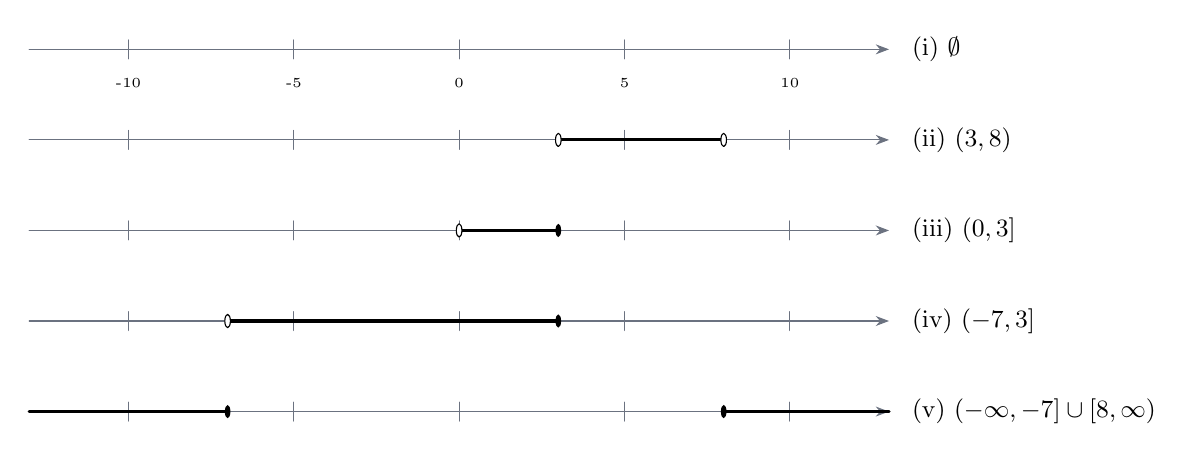
\begin{tikzpicture}[xscale=0.42,yscale=1]
\foreach \r/\lab in {0/{(i) $\emptyset$}, 1/{(ii) $(3,8)$}, 2/{(iii) $(0,3]$},
                     3/{(iv) $(-7,3]$}, 4/{(v) $(-\infty,-7]\cup[8,\infty)$}}{
  \draw[-Stealth,gray] (-13,-1.15*\r)--(13,-1.15*\r);
  \node[right,align=left] at (13.4,-1.15*\r) {\small \lab};
  \foreach \t in {-10,-5,0,5,10}{\draw[gray](\t,-1.15*\r-0.12)--(\t,-1.15*\r+0.12);}
}
\foreach \t in {-10,-5,0,5,10}{\node[below] at (\t,-0.25){\tiny \t};}
% (ii) (3,8)
\draw[very thick] (3,-1.15)--(8,-1.15);
\draw[fill=white] (3,-1.15) circle(2.4pt); \draw[fill=white] (8,-1.15) circle(2.4pt);
% (iii) (0,3]
\draw[very thick] (0,-2.30)--(3,-2.30);
\draw[fill=white] (0,-2.30) circle(2.4pt); \fill (3,-2.30) circle(2.4pt);
% (iv) (-7,3]
\draw[very thick] (-7,-3.45)--(3,-3.45);
\draw[fill=white] (-7,-3.45) circle(2.4pt); \fill (3,-3.45) circle(2.4pt);
% (v)
\draw[very thick] (-13,-4.60)--(-7,-4.60); \fill (-7,-4.60) circle(2.4pt);
\draw[very thick] (8,-4.60)--(13,-4.60); \fill (8,-4.60) circle(2.4pt);
\end{tikzpicture}
\caption{The five answers. A hollow circle marks an excluded endpoint and a solid one an included endpoint.}
\end{figure}

\begin{note}
Endpoints are where marks are lost. Whenever a set is subtracted or complemented, every
$<$ becomes $\geq$ and every $\leq$ becomes $>$ at that endpoint. In (ii) the point $3$
is in $A$, so removing $A$ removes $3$ as well and the answer opens at $3$; in (v) the
point $8$ is \emph{not} in $B$, so it survives into the complement and the answer closes
at $8$.
\end{note}
\end{solution}

\begin{problem}
Let $\mathbb{R}$ be the universal set, $A=(-7,3]$ and $B=(0,8)$. Illustrate De Morgan's
laws using $A$ and $B$.
\end{problem}

\begin{solution}
There are two laws, and each is checked by working out both sides separately and
comparing.

\textbf{First law: $(A\cup B)^c=A^c\cap B^c$.}

\emph{Left-hand side.} $A\cup B=(-7,3]\cup(0,8)=(-7,8)$, since the two intervals
overlap between $0$ and $3$. Hence
$$(A\cup B)^c=(-\infty,-7]\cup[8,\infty).$$

\emph{Right-hand side.}
$$A^c=(-\infty,-7]\cup(3,\infty),\qquad B^c=(-\infty,0]\cup[8,\infty).$$
Intersecting these means taking the points common to both. Below $-7$ both hold; between
$-7$ and $0$ only $B^c$ holds; between $3$ and $8$ only $A^c$ holds; from $8$ upwards
both hold again. So
$$A^c\cap B^c=(-\infty,-7]\cup[8,\infty).$$

The two sides agree. $\checkmark$

\textbf{Second law: $(A\cap B)^c=A^c\cup B^c$.}

\emph{Left-hand side.} $A\cap B=(-7,3]\cap(0,8)=(0,3]$, so
$$(A\cap B)^c=(-\infty,0]\cup(3,\infty).$$

\emph{Right-hand side.} Taking the union of $A^c$ and $B^c$ from above, everything below
$0$ is covered by $B^c$ and everything above $3$ by $A^c$, leaving only $(0,3]$
uncovered:
$$A^c\cup B^c=(-\infty,0]\cup(3,\infty).$$

The two sides agree. $\checkmark$

\begin{figure}[H]
\centering
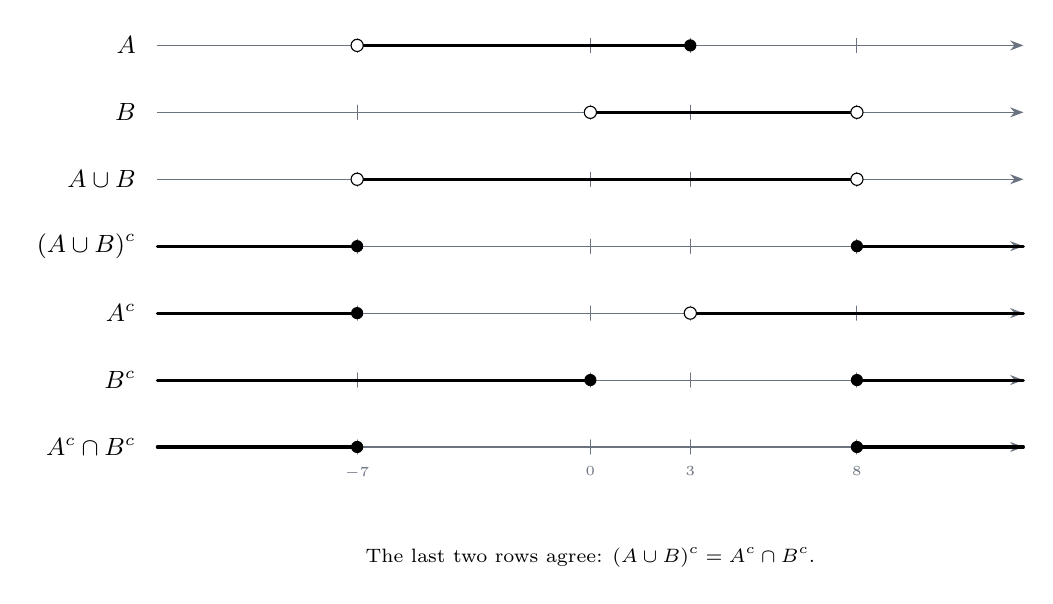
\begin{tikzpicture}
\draw[-Stealth,gray](0.000,-0.0)--(11.000,-0.0);
\draw[gray](2.538,-0.090)--(2.538,0.090);
\draw[gray](5.500,-0.090)--(5.500,0.090);
\draw[gray](6.769,-0.090)--(6.769,0.090);
\draw[gray](8.885,-0.090)--(8.885,0.090);
\draw[very thick](2.538,-0.0)--(6.769,-0.0);
\draw[fill=white](2.538,-0.0) circle(2.2pt);
\fill (6.769,-0.0) circle(2.2pt);
\node[left,font=\small] at (-0.150,-0.0) {$A$};
\draw[-Stealth,gray](0.000,-0.85)--(11.000,-0.85);
\draw[gray](2.538,-0.940)--(2.538,-0.760);
\draw[gray](5.500,-0.940)--(5.500,-0.760);
\draw[gray](6.769,-0.940)--(6.769,-0.760);
\draw[gray](8.885,-0.940)--(8.885,-0.760);
\draw[very thick](5.500,-0.85)--(8.885,-0.85);
\draw[fill=white](5.500,-0.85) circle(2.2pt);
\draw[fill=white](8.885,-0.85) circle(2.2pt);
\node[left,font=\small] at (-0.150,-0.85) {$B$};
\draw[-Stealth,gray](0.000,-1.7)--(11.000,-1.7);
\draw[gray](2.538,-1.790)--(2.538,-1.610);
\draw[gray](5.500,-1.790)--(5.500,-1.610);
\draw[gray](6.769,-1.790)--(6.769,-1.610);
\draw[gray](8.885,-1.790)--(8.885,-1.610);
\draw[very thick](2.538,-1.7)--(8.885,-1.7);
\draw[fill=white](2.538,-1.7) circle(2.2pt);
\draw[fill=white](8.885,-1.7) circle(2.2pt);
\node[left,font=\small] at (-0.150,-1.7) {$A\cup B$};
\draw[-Stealth,gray](0.000,-2.55)--(11.000,-2.55);
\draw[gray](2.538,-2.640)--(2.538,-2.460);
\draw[gray](5.500,-2.640)--(5.500,-2.460);
\draw[gray](6.769,-2.640)--(6.769,-2.460);
\draw[gray](8.885,-2.640)--(8.885,-2.460);
\draw[very thick](0.000,-2.55)--(2.538,-2.55);
\fill (2.538,-2.55) circle(2.2pt);
\draw[very thick](8.885,-2.55)--(11.000,-2.55);
\fill (8.885,-2.55) circle(2.2pt);
\node[left,font=\small] at (-0.150,-2.55) {$(A\cup B)^c$};
\draw[-Stealth,gray](0.000,-3.4)--(11.000,-3.4);
\draw[gray](2.538,-3.490)--(2.538,-3.310);
\draw[gray](5.500,-3.490)--(5.500,-3.310);
\draw[gray](6.769,-3.490)--(6.769,-3.310);
\draw[gray](8.885,-3.490)--(8.885,-3.310);
\draw[very thick](0.000,-3.4)--(2.538,-3.4);
\fill (2.538,-3.4) circle(2.2pt);
\draw[very thick](6.769,-3.4)--(11.000,-3.4);
\draw[fill=white](6.769,-3.4) circle(2.2pt);
\node[left,font=\small] at (-0.150,-3.4) {$A^c$};
\draw[-Stealth,gray](0.000,-4.25)--(11.000,-4.25);
\draw[gray](2.538,-4.340)--(2.538,-4.160);
\draw[gray](5.500,-4.340)--(5.500,-4.160);
\draw[gray](6.769,-4.340)--(6.769,-4.160);
\draw[gray](8.885,-4.340)--(8.885,-4.160);
\draw[very thick](0.000,-4.25)--(5.500,-4.25);
\fill (5.500,-4.25) circle(2.2pt);
\draw[very thick](8.885,-4.25)--(11.000,-4.25);
\fill (8.885,-4.25) circle(2.2pt);
\node[left,font=\small] at (-0.150,-4.25) {$B^c$};
\draw[-Stealth,gray](0.000,-5.1)--(11.000,-5.1);
\draw[gray](2.538,-5.190)--(2.538,-5.010);
\draw[gray](5.500,-5.190)--(5.500,-5.010);
\draw[gray](6.769,-5.190)--(6.769,-5.010);
\draw[gray](8.885,-5.190)--(8.885,-5.010);
\draw[very thick](0.000,-5.1)--(2.538,-5.1);
\fill (2.538,-5.1) circle(2.2pt);
\draw[very thick](8.885,-5.1)--(11.000,-5.1);
\fill (8.885,-5.1) circle(2.2pt);
\node[left,font=\small] at (-0.150,-5.1) {$A^c\cap B^c$};
\node[below,gray,font=\tiny] at (2.538,-5.230) {$-7$};
\node[below,gray,font=\tiny] at (5.500,-5.230) {$0$};
\node[below,gray,font=\tiny] at (6.769,-5.230) {$3$};
\node[below,gray,font=\tiny] at (8.885,-5.230) {$8$};
\node[font=\scriptsize] at (5.5,-6.5) {The last two rows agree: $(A\cup B)^c=A^c\cap B^c$.};
\end{tikzpicture}

\vspace{1.6em}

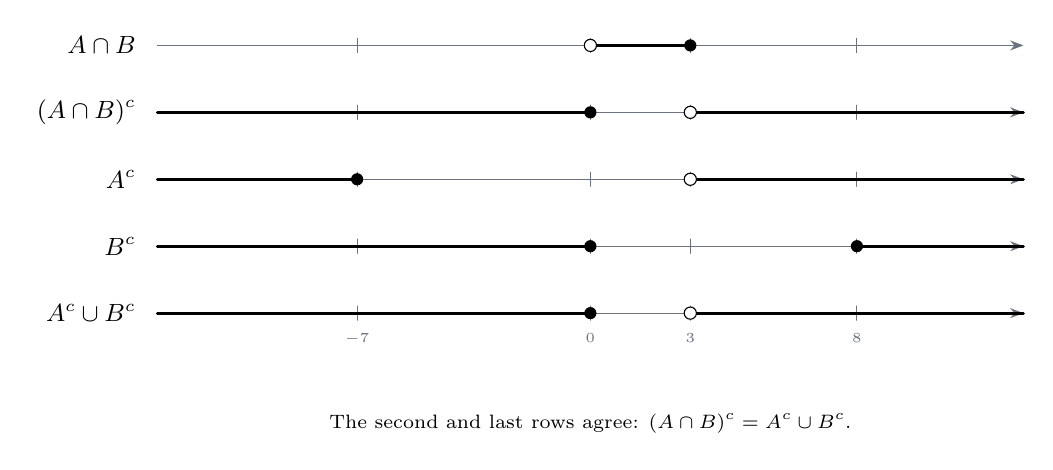
\begin{tikzpicture}
\draw[-Stealth,gray](0.000,-0.0)--(11.000,-0.0);
\draw[gray](2.538,-0.090)--(2.538,0.090);
\draw[gray](5.500,-0.090)--(5.500,0.090);
\draw[gray](6.769,-0.090)--(6.769,0.090);
\draw[gray](8.885,-0.090)--(8.885,0.090);
\draw[very thick](5.500,-0.0)--(6.769,-0.0);
\draw[fill=white](5.500,-0.0) circle(2.2pt);
\fill (6.769,-0.0) circle(2.2pt);
\node[left,font=\small] at (-0.150,-0.0) {$A\cap B$};
\draw[-Stealth,gray](0.000,-0.85)--(11.000,-0.85);
\draw[gray](2.538,-0.940)--(2.538,-0.760);
\draw[gray](5.500,-0.940)--(5.500,-0.760);
\draw[gray](6.769,-0.940)--(6.769,-0.760);
\draw[gray](8.885,-0.940)--(8.885,-0.760);
\draw[very thick](0.000,-0.85)--(5.500,-0.85);
\fill (5.500,-0.85) circle(2.2pt);
\draw[very thick](6.769,-0.85)--(11.000,-0.85);
\draw[fill=white](6.769,-0.85) circle(2.2pt);
\node[left,font=\small] at (-0.150,-0.85) {$(A\cap B)^c$};
\draw[-Stealth,gray](0.000,-1.7)--(11.000,-1.7);
\draw[gray](2.538,-1.790)--(2.538,-1.610);
\draw[gray](5.500,-1.790)--(5.500,-1.610);
\draw[gray](6.769,-1.790)--(6.769,-1.610);
\draw[gray](8.885,-1.790)--(8.885,-1.610);
\draw[very thick](0.000,-1.7)--(2.538,-1.7);
\fill (2.538,-1.7) circle(2.2pt);
\draw[very thick](6.769,-1.7)--(11.000,-1.7);
\draw[fill=white](6.769,-1.7) circle(2.2pt);
\node[left,font=\small] at (-0.150,-1.7) {$A^c$};
\draw[-Stealth,gray](0.000,-2.55)--(11.000,-2.55);
\draw[gray](2.538,-2.640)--(2.538,-2.460);
\draw[gray](5.500,-2.640)--(5.500,-2.460);
\draw[gray](6.769,-2.640)--(6.769,-2.460);
\draw[gray](8.885,-2.640)--(8.885,-2.460);
\draw[very thick](0.000,-2.55)--(5.500,-2.55);
\fill (5.500,-2.55) circle(2.2pt);
\draw[very thick](8.885,-2.55)--(11.000,-2.55);
\fill (8.885,-2.55) circle(2.2pt);
\node[left,font=\small] at (-0.150,-2.55) {$B^c$};
\draw[-Stealth,gray](0.000,-3.4)--(11.000,-3.4);
\draw[gray](2.538,-3.490)--(2.538,-3.310);
\draw[gray](5.500,-3.490)--(5.500,-3.310);
\draw[gray](6.769,-3.490)--(6.769,-3.310);
\draw[gray](8.885,-3.490)--(8.885,-3.310);
\draw[very thick](0.000,-3.4)--(5.500,-3.4);
\fill (5.500,-3.4) circle(2.2pt);
\draw[very thick](6.769,-3.4)--(11.000,-3.4);
\draw[fill=white](6.769,-3.4) circle(2.2pt);
\node[left,font=\small] at (-0.150,-3.4) {$A^c\cup B^c$};
\node[below,gray,font=\tiny] at (2.538,-3.530) {$-7$};
\node[below,gray,font=\tiny] at (5.500,-3.530) {$0$};
\node[below,gray,font=\tiny] at (6.769,-3.530) {$3$};
\node[below,gray,font=\tiny] at (8.885,-3.530) {$8$};
\node[font=\scriptsize] at (5.5,-4.8) {The second and last rows agree: $(A\cap B)^c=A^c\cup B^c$.};
\end{tikzpicture}
\caption{De Morgan's laws on the number line, with $A=(-7,3]$ and $B=(0,8)$. A solid dot is an included endpoint and a hollow one excluded. Each law is read by comparing two rows: build the left-hand side from the top, build the right-hand side separately, and see that the shaded parts coincide.}
\end{figure}


\begin{note}
In words: the complement of a union is the intersection of the complements, and the
complement of an intersection is the union of the complements. The operation flips when
it passes through the complement sign, and that flip is the whole content of both laws.
\end{note}
\end{solution}

\begin{problem}
Express each of the following in the form $\frac{a}{b}$, where $a,b\in\mathbb{Z}$,
$b\neq 0$, and the fraction is in its simplest form.
\quad (i) $1.25$, \quad (ii) $0.666\cdots$, \quad (iii) $2.24\overline{13}$, \quad
(iv) $0.818181818\cdots$, \quad (v) $-2.\overline{71}$, \quad (vi) $0.0\overline{321}$.
\end{problem}

\begin{solution}
A terminating decimal is written straight down over a power of ten. A recurring one needs
the standard trick: multiply by powers of ten so that two copies have the same recurring
tail, then subtract to cancel it.

\textbf{(i).} Terminating, two decimal places:
$$1.25=\frac{125}{100}=\frac{5}{4}.$$

\textbf{(ii).} Let $x=0.666\cdots$, with one recurring digit. Multiply by $10$:
$$10x=6.666\cdots$$
$$10x-x=6.666\cdots-0.666\cdots=6$$
$$9x=6\quad\implies\quad x=\frac{6}{9}=\frac{2}{3}.$$

\textbf{(iii).} $x=2.24131313\cdots$. Here two digits ($24$) come before the recurring
part and two digits ($13$) recur. Multiply by $10^2$ to clear the non-recurring part, and
by $10^{2+2}$ to move one whole cycle further:
$$100x=224.131313\cdots,\qquad 10000x=22413.131313\cdots$$
Subtracting kills the identical tails:
$$9900x=22413-224=22189\quad\implies\quad x=\frac{22189}{9900}.$$
Since $22189$ is prime, no cancelling is possible and this is already simplest.

\textbf{(iv).} $x=0.818181\cdots$, two recurring digits:
$$100x=81.8181\cdots$$
$$99x=81\quad\implies\quad x=\frac{81}{99}=\frac{9}{11}.$$

\textbf{(v).} Deal with the size first and put the sign back at the end. Let
$x=2.717171\cdots$:
$$100x=271.7171\cdots$$
$$99x=271-2=269\quad\implies\quad x=\frac{269}{99},$$
$$\therefore\quad -2.\overline{71}=-\frac{269}{99}.$$

\textbf{(vi).} $x=0.0321321321\cdots$, with one digit ($0$) before the recurrence and
three digits ($321$) recurring:
$$10x=0.321321\cdots,\qquad 10000x=321.321321\cdots$$
$$9990x=321\quad\implies\quad x=\frac{321}{9990}=\frac{107}{3330},$$
after dividing numerator and denominator by $3$.

\begin{note}
The number of $9$s in the denominator equals the number of recurring digits, and each
non-recurring decimal place adds a $0$ after them. Two recurring digits with none before
gives $99$, as in (iv); three recurring digits with one before gives $9990$, as in (vi);
two and two gives $9900$, as in (iii). Recognising the pattern is a useful check on the
subtraction.
\end{note}

\begin{note}
The fact that every one of these is a fraction of whole numbers is exactly what makes
them \emph{rational} numbers. A decimal that neither terminates nor recurs --- such as
$\pi$ or $\sqrt{2}$ --- cannot be caught by this method, and is irrational.
\end{note}
\end{solution}

\begin{problem}
Simplify each of the following.
\quad (i) $\sqrt{36}+\sqrt{64}$, \quad (ii) $7\sqrt{3}+\sqrt{12}$, \quad
(iii) $\sqrt{20}+2\sqrt{45}-\sqrt{80}$, \quad (iv) $3\sqrt{27}-\sqrt{48}+2\sqrt{75}$,
\quad (v) $\sqrt{72}-8\sqrt{3}+3\sqrt{48}$, \quad (vi) $\frac{3\sqrt{28}}{2\sqrt{175}}$.
\end{problem}

\begin{solution}
The method throughout is to pull the largest square factor out of each root, after which
like terms can be collected.

\textbf{(i).} Both are exact squares:
$$\sqrt{36}+\sqrt{64}=6+8=14.$$

\textbf{(ii).} $12=4\times 3$, so $\sqrt{12}=2\sqrt{3}$:
$$7\sqrt{3}+2\sqrt{3}=9\sqrt{3}.$$

\textbf{(iii).} Break each root down to a multiple of $\sqrt{5}$:
$$\sqrt{20}=\sqrt{4\times 5}=2\sqrt{5},\qquad
\sqrt{45}=\sqrt{9\times 5}=3\sqrt{5},\qquad
\sqrt{80}=\sqrt{16\times 5}=4\sqrt{5}.$$
$$\therefore\quad 2\sqrt{5}+2(3\sqrt{5})-4\sqrt{5}=2\sqrt{5}+6\sqrt{5}-4\sqrt{5}
=4\sqrt{5}.$$

\textbf{(iv).} All three reduce to multiples of $\sqrt{3}$:
$$\sqrt{27}=3\sqrt{3},\qquad \sqrt{48}=4\sqrt{3},\qquad \sqrt{75}=5\sqrt{3}.$$
$$\therefore\quad 3(3\sqrt{3})-4\sqrt{3}+2(5\sqrt{3})=9\sqrt{3}-4\sqrt{3}+10\sqrt{3}
=15\sqrt{3}.$$

\textbf{(v).} This time two different surds appear:
$$\sqrt{72}=\sqrt{36\times 2}=6\sqrt{2},\qquad \sqrt{48}=4\sqrt{3}.$$
$$\sqrt{72}-8\sqrt{3}+3\sqrt{48}=6\sqrt{2}-8\sqrt{3}+12\sqrt{3}=6\sqrt{2}+4\sqrt{3}.$$
The $\sqrt{2}$ and $\sqrt{3}$ terms cannot be combined, so this is the final answer.

\textbf{(vi).} Simplify each root before dividing:
$$\sqrt{28}=2\sqrt{7},\qquad \sqrt{175}=\sqrt{25\times 7}=5\sqrt{7}.$$
$$\frac{3\sqrt{28}}{2\sqrt{175}}=\frac{3\left(2\sqrt{7}\right)}{2\left(5\sqrt{7}\right)}
=\frac{6\sqrt{7}}{10\sqrt{7}}=\frac{6}{10}=\frac{3}{5}.$$
The surds cancel completely, leaving a rational number.

\begin{note}
Only \emph{like} surds may be added, exactly as with algebraic terms: $6\sqrt{2}$ and
$4\sqrt{3}$ can no more be combined than $6a$ and $4b$. Writing $6\sqrt{2}+4\sqrt{3}=
10\sqrt{5}$ is the error to guard against --- and it is easy to spot, since
$6\sqrt{2}+4\sqrt{3}\approx 15.4$ while $10\sqrt{5}\approx 22.4$.
\end{note}
\end{solution}

\begin{problem}
Rationalise the denominator in each of the following.
\quad (i) $\frac{3}{\sqrt{5}}$, \quad (ii) $\frac{2}{3-\sqrt{3}}$, \quad
(iii) $\frac{3\sqrt{2}}{2+\sqrt{5}}$, \quad
(iv) $\frac{\sqrt{3}-\sqrt{7}}{\sqrt{3}+\sqrt{7}}$, \quad
(v) $\frac{x-y}{\sqrt{x}-\sqrt{y}}$, \quad
(vi) $\frac{h}{\sqrt{x+h}-\sqrt{x}}$.
\end{problem}

\begin{solution}
For a single surd, multiply top and bottom by that surd. For a two-term denominator,
multiply by its \textbf{conjugate} --- the same expression with the middle sign reversed
--- because $(a-b)(a+b)=a^2-b^2$ removes the roots.

\textbf{(i).}
$$\frac{3}{\sqrt{5}}\times\frac{\sqrt{5}}{\sqrt{5}}=\frac{3\sqrt{5}}{5}.$$

\textbf{(ii).} The conjugate of $3-\sqrt{3}$ is $3+\sqrt{3}$:
$$\frac{2}{3-\sqrt{3}}\times\frac{3+\sqrt{3}}{3+\sqrt{3}}
=\frac{2\left(3+\sqrt{3}\right)}{9-3}=\frac{2\left(3+\sqrt{3}\right)}{6}
=\frac{3+\sqrt{3}}{3}.$$

\textbf{(iii).} The conjugate of $2+\sqrt{5}$ is $2-\sqrt{5}$, and note that
$4-5=-1$:
$$\frac{3\sqrt{2}}{2+\sqrt{5}}\times\frac{2-\sqrt{5}}{2-\sqrt{5}}
=\frac{3\sqrt{2}\left(2-\sqrt{5}\right)}{4-5}
=\frac{6\sqrt{2}-3\sqrt{10}}{-1}=3\sqrt{10}-6\sqrt{2}.$$
The negative denominator flips both signs, which is easy to overlook.

\textbf{(iv).} Multiply top and bottom by $\sqrt{3}-\sqrt{7}$:
$$\frac{\sqrt{3}-\sqrt{7}}{\sqrt{3}+\sqrt{7}}\times
\frac{\sqrt{3}-\sqrt{7}}{\sqrt{3}-\sqrt{7}}
=\frac{\left(\sqrt{3}-\sqrt{7}\right)^2}{3-7}.$$
Expanding the numerator,
$$\left(\sqrt{3}-\sqrt{7}\right)^2=3-2\sqrt{21}+7=10-2\sqrt{21},$$
so
$$=\frac{10-2\sqrt{21}}{-4}=\frac{2\sqrt{21}-10}{4}=\frac{\sqrt{21}-5}{2}.$$

\textbf{(v).} The conjugate of $\sqrt{x}-\sqrt{y}$ is $\sqrt{x}+\sqrt{y}$:
$$\frac{x-y}{\sqrt{x}-\sqrt{y}}\times\frac{\sqrt{x}+\sqrt{y}}{\sqrt{x}+\sqrt{y}}
=\frac{(x-y)\left(\sqrt{x}+\sqrt{y}\right)}{x-y}=\sqrt{x}+\sqrt{y},$$
cancelling the factor $x-y$ top and bottom.

\textbf{(vi).}
$$\frac{h}{\sqrt{x+h}-\sqrt{x}}\times\frac{\sqrt{x+h}+\sqrt{x}}{\sqrt{x+h}+\sqrt{x}}
=\frac{h\left(\sqrt{x+h}+\sqrt{x}\right)}{(x+h)-x}
=\frac{h\left(\sqrt{x+h}+\sqrt{x}\right)}{h}=\sqrt{x+h}+\sqrt{x}.$$

\begin{note}
Part (vi) is not an idle exercise. Turn it upside down and it becomes
$$\frac{\sqrt{x+h}-\sqrt{x}}{h}=\frac{1}{\sqrt{x+h}+\sqrt{x}},$$
which is precisely the manipulation needed to differentiate $\sqrt{x}$ from first
principles. Before the surd is rationalised, letting $h\to 0$ gives $\frac{0}{0}$; after,
it gives $\frac{1}{2\sqrt{x}}$ at once.
\end{note}
\end{solution}

\begin{problem}
Rationalise the denominator and simplify.
\quad (i) $\frac{4}{\sqrt{2}}+\sqrt{8}$, \quad
(ii) $\frac{8}{3+\sqrt{5}}+\sqrt{45}$, \quad
(iii) $\frac{\sqrt{3}-\sqrt{7}}{\sqrt{3}+\sqrt{7}}+\sqrt{21}$.
\end{problem}

\begin{solution}
\textbf{(i).} Rationalise the first term and simplify the second:
$$\frac{4}{\sqrt{2}}=\frac{4\sqrt{2}}{2}=2\sqrt{2},\qquad \sqrt{8}=2\sqrt{2}.$$
$$\therefore\quad 2\sqrt{2}+2\sqrt{2}=4\sqrt{2}.$$

\textbf{(ii).} The conjugate of $3+\sqrt{5}$ is $3-\sqrt{5}$, and $9-5=4$:
$$\frac{8}{3+\sqrt{5}}\times\frac{3-\sqrt{5}}{3-\sqrt{5}}
=\frac{8\left(3-\sqrt{5}\right)}{4}=2\left(3-\sqrt{5}\right)=6-2\sqrt{5}.$$
Also $\sqrt{45}=3\sqrt{5}$. Adding:
$$6-2\sqrt{5}+3\sqrt{5}=6+\sqrt{5}.$$

\textbf{(iii).} The first term was rationalised in the previous question to
$\frac{\sqrt{21}-5}{2}$. Adding $\sqrt{21}$ over a common denominator:
$$\frac{\sqrt{21}-5}{2}+\sqrt{21}=\frac{\sqrt{21}-5+2\sqrt{21}}{2}
=\frac{3\sqrt{21}-5}{2}.$$

\begin{note}
Rationalise first, then combine. Attempting to add $\frac{8}{3+\sqrt{5}}$ to $\sqrt{45}$
over a common denominator before clearing the surd produces a far messier expression
that has to be rationalised in the end anyway.
\end{note}
\end{solution}

\begin{problem}
\begin{enumerate}
\item[(a).] Simplify, leaving each answer in the standard form $a+bi$ with
$a,b\in\mathbb{R}$:
\quad (i) $(2+3i)-(-7+6i)$, \quad (ii) $(3+4i)+(6-5i)$, \quad (iii) $(-2+3i)^2$, \quad
(iv) $(2+i)(-1+2i)(4-3i)$, \quad (v) $\frac{2-3i}{1-2i}$, \quad
(vi) $\frac{(-2+3i)^2}{1+2i}$.
\item[(b).] Simplify \quad (i) $i^{11}$, \quad (ii) $i^{102}$, \quad (iii) $i^{250}$,
\quad (iv) $i^{900}$.
\end{enumerate}
\end{problem}

\begin{solution}
Throughout, $i^2=-1$ is the only new fact; everything else is ordinary algebra.

\textbf{(a)(i).} Subtracting a bracket changes both signs inside it:
$$(2+3i)-(-7+6i)=2+3i+7-6i=9-3i.$$

\textbf{(ii).} Collect real with real and imaginary with imaginary:
$$(3+4i)+(6-5i)=(3+6)+(4-5)i=9-i.$$

\textbf{(iii).} Expand as a square, then replace $i^2$ by $-1$:
$$(-2+3i)^2=4-12i+9i^2=4-12i-9=-5-12i.$$

\textbf{(iv).} Multiply two factors at a time:
$$(2+i)(-1+2i)=-2+4i-i+2i^2=-2+3i-2=-4+3i.$$
$$(-4+3i)(4-3i)=-16+12i+12i-9i^2=-16+24i+9=-7+24i.$$

\textbf{(v).} To divide, multiply top and bottom by the conjugate of the denominator.
The conjugate of $1-2i$ is $1+2i$, and $(1-2i)(1+2i)=1+4=5$:
$$\frac{2-3i}{1-2i}\times\frac{1+2i}{1+2i}=\frac{2+4i-3i-6i^2}{5}
=\frac{2+i+6}{5}=\frac{8+i}{5}=\frac{8}{5}+\frac{1}{5}i.$$

\textbf{(vi).} The numerator was found in (iii) to be $-5-12i$. The conjugate of
$1+2i$ is $1-2i$, and $(1+2i)(1-2i)=5$:
$$\frac{-5-12i}{1+2i}\times\frac{1-2i}{1-2i}=\frac{-5+10i-12i+24i^2}{5}
=\frac{-5-2i-24}{5}=\frac{-29-2i}{5}=-\frac{29}{5}-\frac{2}{5}i.$$

\textbf{(b).} The powers of $i$ repeat in a cycle of four:
$$i^1=i,\qquad i^2=-1,\qquad i^3=-i,\qquad i^4=1,$$
and then the pattern begins again. So divide the index by $4$ and keep only the
remainder.

$$\text{(i) } 11=4(2)+3\quad\implies\quad i^{11}=i^3=-i.$$
$$\text{(ii) } 102=4(25)+2\quad\implies\quad i^{102}=i^2=-1.$$
$$\text{(iii) } 250=4(62)+2\quad\implies\quad i^{250}=i^2=-1.$$
$$\text{(iv) } 900=4(225)+0\quad\implies\quad i^{900}=i^0=1.$$

\begin{note}
For (b) there is no need to work out the power itself --- only the remainder on division
by $4$ matters. A remainder of $0$ gives $1$, of $1$ gives $i$, of $2$ gives $-1$ and of
$3$ gives $-i$.
\end{note}
\end{solution}

\begin{problem}
Given $z_1=3-2i$, $z_2=-1+i$ and $z_3=3+2i$, evaluate each of the following, leaving the
answer in the form $a+bi$:
\quad (i) $\frac{2z_1-5z_3}{\bar{z_3}}$, \quad (ii) $\frac{\bar{z_2}z_1}{z_3}$, \quad
(iii) $\frac{\left(z_2\right)^2}{\bar{z_1}}$.
\end{problem}

\begin{solution}
First write down the conjugates, obtained by changing the sign of the imaginary part:
$$\bar{z_1}=3+2i,\qquad \bar{z_2}=-1-i,\qquad \bar{z_3}=3-2i.$$

\textbf{(i).} Numerator first:
$$2z_1-5z_3=2(3-2i)-5(3+2i)=(6-4i)-(15+10i)=-9-14i.$$
Divide by $\bar{z_3}=3-2i$, multiplying top and bottom by its conjugate $3+2i$. Note
$(3-2i)(3+2i)=9+4=13$:
$$\frac{-9-14i}{3-2i}\times\frac{3+2i}{3+2i}=\frac{-27-18i-42i-28i^2}{13}
=\frac{-27-60i+28}{13}=\frac{1-60i}{13}=\frac{1}{13}-\frac{60}{13}i.$$

\textbf{(ii).} Numerator first:
$$\bar{z_2}z_1=(-1-i)(3-2i)=-3+2i-3i+2i^2=-3-i-2=-5-i.$$
Divide by $z_3=3+2i$, using the conjugate $3-2i$ and $(3+2i)(3-2i)=13$:
$$\frac{-5-i}{3+2i}\times\frac{3-2i}{3-2i}=\frac{-15+10i-3i+2i^2}{13}
=\frac{-15+7i-2}{13}=\frac{-17+7i}{13}=-\frac{17}{13}+\frac{7}{13}i.$$

\textbf{(iii).} Numerator first:
$$\left(z_2\right)^2=(-1+i)^2=1-2i+i^2=1-2i-1=-2i.$$
Divide by $\bar{z_1}=3+2i$:
$$\frac{-2i}{3+2i}\times\frac{3-2i}{3-2i}=\frac{-6i+4i^2}{13}=\frac{-4-6i}{13}
=-\frac{4}{13}-\frac{6}{13}i.$$

\begin{note}
Here $z_3=3+2i$ happens to be the conjugate of $z_1=3-2i$, so $\bar{z_3}=z_1$ and
$\bar{z_1}=z_3$. Noticing that at the start halves the writing. It also explains why
every denominator came out as $13$: in each case the product was $(3+2i)(3-2i)=3^2+2^2$.
\end{note}
\end{solution}

\begin{problem}
\begin{enumerate}
\item[(a).] Solve for the real numbers $x$ and $y$:
\quad (i) $x+6+2yi=6-5i$, \quad (ii) $4x+(3y+4)i=21+7i$, \quad
(iii) $6+3i=4i-30(x+yi)$.
\item[(b).] Given that $\frac{5-2i}{z}=2+i$, find $z$ in the form $a+bi$.
\end{enumerate}
\end{problem}

\begin{solution}
Two complex numbers are equal precisely when their real parts are equal \emph{and} their
imaginary parts are equal. Each equation therefore splits into two real equations.

\textbf{(a)(i).} Comparing real parts and then imaginary parts:
$$x+6=6\quad\implies\quad x=0,$$
$$2y=-5\quad\implies\quad y=-\frac{5}{2}.$$

\textbf{(ii).}
$$4x=21\quad\implies\quad x=\frac{21}{4},$$
$$3y+4=7\quad\implies\quad 3y=3\quad\implies\quad y=1.$$

\textbf{(iii).} First expand the right-hand side and gather it into the form
$a+bi$:
$$4i-30(x+yi)=-30x+(4-30y)i.$$
Now compare with the left-hand side $6+3i$:
$$-30x=6\quad\implies\quad x=-\frac{1}{5},$$
$$4-30y=3\quad\implies\quad 30y=1\quad\implies\quad y=\frac{1}{30}.$$

\textbf{(b).} Rearranging,
$$z=\frac{5-2i}{2+i}.$$
Multiply top and bottom by the conjugate $2-i$, with $(2+i)(2-i)=4+1=5$:
$$z=\frac{(5-2i)(2-i)}{5}=\frac{10-5i-4i+2i^2}{5}=\frac{10-9i-2}{5}=\frac{8-9i}{5},$$
$$\therefore\quad z=\frac{8}{5}-\frac{9}{5}i.$$

\textbf{Check.} Multiplying back,
$$\left(\frac{8-9i}{5}\right)(2+i)=\frac{16+8i-18i-9i^2}{5}=\frac{16-10i+9}{5}
=\frac{25-10i}{5}=5-2i.\ \checkmark$$

\begin{note}
In (iii) the expansion must be done \emph{before} comparing parts. Reading off
$6=4i$ and $3i=-30(x+yi)$, as though the terms could be matched in the order written,
gives nonsense --- the real part of the right-hand side is $-30x$, which is not visible
until the bracket is multiplied out.
\end{note}
\end{solution}

\section{Functions}

A function is a rule that turns one number into another. Almost every later chapter
studies some particular family of them, so it is worth being exact about what the word
means and what can go wrong.

\subsection{Ordered pairs and relations}

\begin{definition}
The \textbf{Cartesian product} of sets $X$ and $Y$, written $X\times Y$ and read
``$X$ cross $Y$'', is the set of all ordered pairs with first entry from $X$ and
second from $Y$:
$$X\times Y=\{(x,y) : x\in X,\ y\in Y\}.$$
\end{definition}

The pairs are \emph{ordered}: $(1,a)$ and $(a,1)$ are different, and in $X\times X$ the
pairs $(1,2)$ and $(2,1)$ are different too.

\begin{example}
Let $A=\{1,2\}$ and $B=\{a,b,c\}$. Write down $A\times B$ and $A\times A$.
\end{example}

\begin{solution}
Take each element of the first set with each element of the second, in turn:
$$A\times B=\{(1,a),\,(1,b),\,(1,c),\,(2,a),\,(2,b),\,(2,c)\}.$$
For $A\times A$ the same rule applies, with $A$ playing both parts:
$$A\times A=\{(1,1),\,(1,2),\,(2,1),\,(2,2)\}.$$

\textbf{Count them as a check.} If $|X|=m$ and $|Y|=n$ then $|X\times Y|=mn$, because
each of the $m$ first entries can be paired with each of the $n$ second entries. Here
$|A\times B|=2\times 3=6$ and $|A\times A|=2\times 2=4$, which matches what was
listed.

That check earns its place: $(1,2)$ and $(2,1)$ are both in $A\times A$ and it is easy
to write one and forget the other, leaving three pairs where there should be four.
\end{solution}

\begin{definition}
A \textbf{relation} $R$ from $X$ to $Y$ is any subset of $X\times Y$. If
$(x,y)\in R$ we say $x$ is related to $y$ and write $x\,R\,y$.
\end{definition}

So a relation is just a rule that links some elements of one set to some elements of
another. $X$ is the \textbf{input set} and $Y$ the \textbf{output set}.

\subsubsection{Classifying relations}

Relations are described by how many arrows leave and arrive at each element.

\begin{table}[H]
\centering
\begin{tabular}{|l|l|}
\hline
Type & Description\\
\hline
One-to-one & each input goes to one output, and no output is used twice\\
Many-to-one & several inputs share the same output\\
One-to-many & one input goes to several outputs\\
Many-to-many & both of the last two happen\\
\hline
\end{tabular}
\caption{The four kinds of relation.}
\end{table}

\begin{example}
Let $X=\{3,5,7\}$ and $Y=\{6,10,14\}$ with the relation ``is a factor of''. Show it on
an arrow diagram and classify it.
\end{example}

\begin{solution}
$3$ divides $6$; $5$ divides $10$; $7$ divides $14$. No other pairs work, since $3$
does not divide $10$ or $14$, and so on.
\begin{figure}[H]
\centering
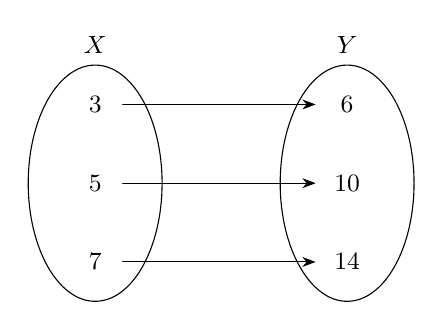
\begin{tikzpicture}
\draw (-1.6,-1.6) ellipse (0.85 and 1.5);
\draw (1.6,-1.6) ellipse (0.85 and 1.5);
\node at (-1.6,0.15) {$X$};
\node at (1.6,0.15) {$Y$};
\foreach \y/\a in {-0.6/3,-1.6/5,-2.6/7}{\node at (-1.6,\y) {$\a$};}
\foreach \y/\b in {-0.6/6,-1.6/10,-2.6/14}{\node at (1.6,\y) {$\b$};}
\foreach \y in {-0.6,-1.6,-2.6}{\draw[-Stealth](-1.25,\y)--(1.2,\y);}
\end{tikzpicture}
\caption{``Is a factor of'' from $X$ to $Y$. One arrow leaves each input and one arrives at each output, so the relation is one-to-one.}
\end{figure}
Every input has exactly one arrow out and every output exactly one arrow in, so the
relation is \textbf{one-to-one}.
\end{solution}

\begin{definition}
For a relation from $X$ to $Y$:
\begin{enumerate}
\item[(i).] the \textbf{domain} is the set of inputs actually used --- the first
entries of the pairs;
\item[(ii).] the \textbf{range} is the set of outputs actually reached --- the second
entries;
\item[(iii).] the \textbf{co-domain} is the whole of $Y$, whether or not every element
of it is reached.
\end{enumerate}
\end{definition}

\begin{note}
The range is always a subset of the co-domain, and often a proper one. The co-domain is
the set you \emph{declared} the outputs would come from; the range is what actually
came out.
\end{note}

\subsection{Functions}

\begin{definition}
A \textbf{function} $f$ from $X$ to $Y$, written $f:X\to Y$, is a relation in which
\emph{every} element of $X$ is assigned to \emph{exactly one} element of $Y$.
\end{definition}

Two conditions, and both matter:

\begin{enumerate}
\item[(i).] \textbf{every} input must be used --- nothing in $X$ is left without an
arrow;
\item[(ii).] each input has \textbf{exactly one} output --- no input has two arrows
leaving it.
\end{enumerate}

So every function is a relation, but not every relation is a function. A one-to-many
relation is never a function, because condition (ii) fails.

We write $y=f(x)$, calling $x$ the \textbf{independent variable} and $y$ the
\textbf{dependent variable}. The value $f(x)$ is read ``$f$ of $x$''.

\begin{note}
$f(x)$ does not mean $f$ multiplied by $x$. It is one symbol meaning ``the output of
$f$ when the input is $x$''.
\end{note}

\begin{example}
The function $f(x)=\frac{x}{2}+7$ is the rule ``halve the input, then add $7$''.
Find $f(4)$, $f(0)$ and $f(-6)$.
\end{example}

\begin{solution}
Substitute each value in turn, keeping the brackets until the last step:
$$f(4)=\frac{4}{2}+7=2+7=9$$
$$f(0)=\frac{0}{2}+7=0+7=7$$
$$f(-6)=\frac{-6}{2}+7=-3+7=4.$$
\end{solution}

\begin{example}
The function $f$ is defined by
$$f(x)=\begin{cases} 2x-3 & \text{for } x<0,\\ 3x+1 & \text{for } x\geq 0.\end{cases}$$
Find $f\!\left(\tfrac{1}{2}\right)$, $f(0)$ and $f(-3)$.
\end{example}

\begin{solution}
This is a \textbf{piecewise} function: which formula applies depends on the input, so
check the condition \emph{first} and only then substitute.

$\tfrac{1}{2}\geq 0$, so use the second line:
$$f\!\left(\tfrac{1}{2}\right)=3\!\left(\tfrac{1}{2}\right)+1=\tfrac{3}{2}+1=\tfrac{5}{2}.$$

$0\geq 0$, so the second line again --- note the condition is $x\geq 0$, not $x>0$:
$$f(0)=3(0)+1=1.$$

$-3<0$, so the first line:
$$f(-3)=2(-3)-3=-6-3=-9.$$

The commonest mistake here is substituting into whichever formula is written first.
Read the condition before choosing the rule.
\end{solution}

\subsection{Composite functions}

\begin{definition}
Given functions $f$ and $g$, the \textbf{composite} $f\circ g$ is defined by
$$(f\circ g)(x)=f\big(g(x)\big).$$
Here $g$ is the \textbf{inside} function and $f$ the \textbf{outside} one.
\end{definition}

Read it from the inside out: apply $g$ first, then feed the answer into $f$. The
notation is the reverse of the order of work, which is what makes it easy to get
backwards.

\begin{example}
Let $f(x)=2x-1$ and $g(x)=3x$. Find
$$\text{(a) } (g\circ f)(x),\qquad \text{(b) } (f\circ g)(x),
\qquad \text{(c) } (f\circ f)(x),\qquad \text{(d) } (g\circ g)(x).$$
\end{example}

\begin{solution}
\textbf{(a)} Inside first: $f(x)=2x-1$. Feed that into $g$, which triples its input:
$$(g\circ f)(x)=g(2x-1)=3(2x-1)=6x-3.$$

\textbf{(b)} Now the other order. Inside is $g(x)=3x$; feed it into $f$, which doubles
and subtracts $1$:
$$(f\circ g)(x)=f(3x)=2(3x)-1=6x-1.$$

\textbf{(c)} $$(f\circ f)(x)=f(2x-1)=2(2x-1)-1=4x-2-1=4x-3.$$

\textbf{(d)} $$(g\circ g)(x)=g(3x)=3(3x)=9x.$$
\end{solution}

\begin{note}
Compare (a) and (b): $6x-3$ against $6x-1$. \textbf{Composition is not commutative} ---
$f\circ g$ and $g\circ f$ are usually different functions. Order matters, and it is not
optional.
\end{note}

\subsection{Odd and even functions}

\begin{definition}
A function $f$ is \textbf{even} if $f(-x)=f(x)$ for every $x$, and \textbf{odd} if
$f(-x)=-f(x)$ for every $x$.
\end{definition}

An even function is unchanged when the sign of the input flips; an odd one changes
sign with it. Graphically, an even function is symmetric about the $y$-axis and an odd
one has rotational symmetry about the origin.

\begin{example}
State whether each function is even, odd, or neither.
\begin{enumerate}
\item[(a).] $f(x)=\frac{x^3-x}{x^2+4}$
\item[(b).] $f(x)=x^4-3x^2+7$
\item[(c).] $f(x)=2x+7$
\end{enumerate}
\end{example}

\begin{solution}
In every case the method is the same: work out $f(-x)$, then compare it with $f(x)$ and
with $-f(x)$.

\textbf{(a)} Replace each $x$ by $-x$, remembering $(-x)^3=-x^3$ and $(-x)^2=x^2$:
$$f(-x)=\frac{(-x)^3-(-x)}{(-x)^2+4}=\frac{-x^3+x}{x^2+4}=-\left(\frac{x^3-x}{x^2+4}\right)=-f(x).$$
So $f$ is \textbf{odd}.

\textbf{(b)} Only even powers appear, and the constant is unaffected:
$$f(-x)=(-x)^4-3(-x)^2+7=x^4-3x^2+7=f(x).$$
So $f$ is \textbf{even}.

\textbf{(c)} $$f(-x)=2(-x)+7=-2x+7.$$
This is not $f(x)=2x+7$, so $f$ is not even. Nor is it $-f(x)=-2x-7$, since the
constants differ. So $f$ is \textbf{neither}.
\end{solution}

\begin{note}
Most functions are neither odd nor even --- those two are special cases, not
alternatives. Part (c) shows how a single constant term can spoil oddness: $2x$ on its
own is odd, but $2x+7$ is not.
\end{note}

\subsection{Inverse of a function}

\begin{definition}
Functions $f$ and $g$ are \textbf{inverses} of each other if
$$(f\circ g)(x)=x\quad\text{and}\quad (g\circ f)(x)=x$$
for all $x$ in the appropriate domains. The inverse of $f$ is written $f^{-1}$.
\end{definition}

The inverse undoes what the function does: put a number in, apply $f$, apply $f^{-1}$,
and you are back where you started.

\begin{note}
$f^{-1}$ does \textbf{not} mean $\frac{1}{f}$. The superscript $-1$ here means
``inverse function'', not ``reciprocal''.
\end{note}

Only a one-to-one function has an inverse. If two different inputs shared an output,
the reverse rule would not know which to return, and so would not be a function.

\begin{remark}
Since the inverse reverses every arrow, the domain and range swap over:
$$\text{domain of } f^{-1}=\text{range of } f,\qquad
\text{range of } f^{-1}=\text{domain of } f.$$
\end{remark}

\begin{example}
Show that $f(x)=\frac{x-3}{2}$ and $g(x)=2x+3$ are inverses of each other.
\end{example}

\begin{solution}
Both composites must come out as $x$; checking only one is not enough in general.
$$(f\circ g)(x)=f(2x+3)=\frac{(2x+3)-3}{2}=\frac{2x}{2}=x$$
$$(g\circ f)(x)=g\!\left(\frac{x-3}{2}\right)=2\!\left(\frac{x-3}{2}\right)+3=(x-3)+3=x.$$
Both give $x$, so $f$ and $g$ are inverses.
\end{solution}

\subsubsection{Finding an inverse}

The method is always the same three steps: write $y=f(x)$, make $x$ the subject, then
swap the letters.

\begin{example}
Find the inverse of $f(x)=\frac{3x+1}{x-2}$, and state its domain.
\end{example}

\begin{solution}
\textbf{Step 1.} Write $y$ for the output:
$$y=\frac{3x+1}{x-2}.$$

\textbf{Step 2.} Make $x$ the subject. Clear the fraction first:
$$y(x-2)=3x+1\quad\implies\quad xy-2y=3x+1.$$
Gather every term containing $x$ on one side and everything else on the other:
$$xy-3x=2y+1\quad\implies\quad x(y-3)=2y+1$$
$$\implies\quad x=\frac{2y+1}{y-3}.$$

\textbf{Step 3.} Swap $x$ and $y$, since the inverse takes the old outputs as its
inputs:
$$f^{-1}(x)=\frac{2x+1}{x-3}.$$

\textbf{Domain.} The inverse is undefined where its denominator vanishes, so
$x\neq 3$; its domain is $\mathbb{R}\setminus\{3\}$. Notice that $3$ is precisely the
value $f$ can never output --- as $x$ grows, $\frac{3x+1}{x-2}$ approaches $3$ without
reaching it. The range of $f$ and the domain of $f^{-1}$ agree, as they must.

\textbf{Check.} $$f\big(f^{-1}(x)\big)
=\frac{3\left(\frac{2x+1}{x-3}\right)+1}{\left(\frac{2x+1}{x-3}\right)-2}
=\frac{\frac{6x+3+x-3}{x-3}}{\frac{2x+1-2x+6}{x-3}}
=\frac{7x}{7}=x. $$
\end{solution}


\subsection{Practice problems}

Tutorial Sheet 2 in full. Work each question before opening the solution.

\begin{problem}
Illustrate each of the following sets of ordered pairs on an arrow diagram. Which of
them are functions? Give a reason in each case.
\begin{enumerate}
\item[(i).] $\{(0,-1),(2,2),(1,-2),(3,0)\}$
\item[(ii).] $\{(1,a),(3,c),(2,b)\}$
\item[(iii).] $\{(1,a),(1,b),(2,c),(1,d)\}$
\item[(iv).] $\{(1,b),(2,b),(3,c),(4,b)\}$
\end{enumerate}
\end{problem}

\begin{solution}
An arrow diagram puts the first components in a left-hand oval and the second components
in a right-hand one, with an arrow from each first component to its partner.

\begin{figure}[H]
\centering
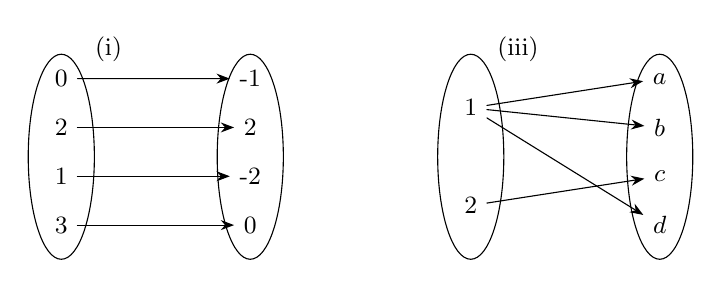
\begin{tikzpicture}[yscale=0.62,xscale=1.0]
% (i)
\begin{scope}[xshift=0cm]
\node at (0.6,2.6) {\small (i)};
\draw (0,0.4) ellipse (0.42 and 2.1);
\draw (2.4,0.4) ellipse (0.42 and 2.1);
\foreach \y/\l in {2/0, 1/2, 0/1, -1/3} {\node (L\l) at (0,\y) {\small \l};}
\foreach \y/\l in {2/{-1}, 1/2, 0/{-2}, -1/0} {\node (R\y) at (2.4,\y) {\small \l};}
\draw[-Stealth] (L0)--(R2); \draw[-Stealth] (L2)--(R1);
\draw[-Stealth] (L1)--(R0); \draw[-Stealth] (L3)--(R-1);
\end{scope}
% (iii)
\begin{scope}[xshift=5.2cm]
\node at (0.6,2.6) {\small (iii)};
\draw (0,0.4) ellipse (0.42 and 2.1);
\draw (2.4,0.4) ellipse (0.42 and 2.1);
\node (P1) at (0,1.4) {\small 1};
\node (P2) at (0,-0.6) {\small 2};
\node (Qa) at (2.4,2) {\small $a$};
\node (Qb) at (2.4,1) {\small $b$};
\node (Qc) at (2.4,0) {\small $c$};
\node (Qd) at (2.4,-1) {\small $d$};
\draw[-Stealth] (P1)--(Qa); \draw[-Stealth] (P1)--(Qb); \draw[-Stealth] (P1)--(Qd);
\draw[-Stealth] (P2)--(Qc);
\end{scope}
\end{tikzpicture}
\caption{Two of the four diagrams. In (i) exactly one arrow leaves each left-hand element; in (iii) three arrows leave the element 1.}
\end{figure}

The test is always the same: a set of ordered pairs is a \textbf{function} when every
first component has \emph{exactly one} arrow leaving it.

\textbf{(i).} The first components are $0$, $2$, $1$, $3$ --- all different, so each has
exactly one arrow. \textbf{It is a function.}

\textbf{(ii).} The first components are $1$, $3$, $2$ --- all different.
\textbf{It is a function.}

\textbf{(iii).} The first component $1$ appears three times, sending $1$ to $a$, to $b$
and to $d$. \textbf{It is not a function}, because a function must give one output for
each input.

\textbf{(iv).} The first components are $1$, $2$, $3$, $4$ --- all different.
\textbf{It is a function}, even though three of them share the output $b$.

\begin{note}
Compare (iii) and (iv). Repetition on the \emph{left} destroys a function; repetition on
the \emph{right} does not. Several inputs are free to share an output --- that is
called many-to-one and is perfectly ordinary --- but one input may never have two
outputs.
\end{note}
\end{solution}

\begin{problem}
For each function, (i) list its domain and range, and (ii) form the inverse function
$f^{-1}$ and list its domain and range.
\begin{enumerate}
\item[(a).] $f=\{(1,5),(2,9),(5,21)\}$
\item[(b).] $f=\{(0,0),(2,8),(-1,-1),(-2,-8)\}$
\end{enumerate}
\end{problem}

\begin{solution}
The domain is the set of first components and the range the set of second components.
The inverse is formed by reversing every pair.

\textbf{(a).}
$$\text{domain of } f=\{1,2,5\},\qquad \text{range of } f=\{5,9,21\}.$$
Reversing each pair,
$$f^{-1}=\{(5,1),(9,2),(21,5)\},$$
$$\text{domain of } f^{-1}=\{5,9,21\},\qquad \text{range of } f^{-1}=\{1,2,5\}.$$

\textbf{(b).}
$$\text{domain of } f=\{-2,-1,0,2\},\qquad \text{range of } f=\{-8,-1,0,8\}.$$
$$f^{-1}=\{(0,0),(8,2),(-1,-1),(-8,-2)\},$$
$$\text{domain of } f^{-1}=\{-8,-1,0,8\},\qquad \text{range of } f^{-1}=\{-2,-1,0,2\}.$$

\begin{note}
The domain of $f^{-1}$ is the range of $f$, and the range of $f^{-1}$ is the domain of
$f$. That swap is not a separate fact to memorise --- it follows immediately from
reversing the pairs, and it is worth using as a check that no pair was dropped.
\end{note}

\begin{note}
Reversing the pairs only produces a \emph{function} if no two pairs of $f$ shared a
second component. Both sets here pass. Had $f$ contained $(1,5)$ and $(2,5)$, the
reversed set would send $5$ to both $1$ and $2$, and $f^{-1}$ would not exist.
\end{note}
\end{solution}

\begin{problem}
\begin{enumerate}
\item[(a).] If
$$f(x)=\begin{cases} 2x-3 & \text{for } x<0,\\ 3x+1 & \text{for } x\geq 0,\end{cases}$$
compute $f\left(\frac{1}{2}\right)$, $f(0)$ and $f(-3)$.
\item[(b).] If
$$f(x)=\begin{cases} -5 & \text{for } x<0,\\ 2x^2+3 & \text{for } 0\leq x\leq 3,\\
5 & \text{for } x>3,\end{cases}$$
compute $f(-5)$, $f\left(\frac{5}{2}\right)$, $f(0)$ and $f(10)$.
\end{enumerate}
\end{problem}

\begin{solution}
With a piecewise function, the first job is always to decide \emph{which line applies},
and only then to substitute.

\textbf{(a).}
$$f\left(\tfrac{1}{2}\right):\quad \tfrac{1}{2}\geq 0,\text{ so use } 3x+1:\qquad
3\left(\tfrac{1}{2}\right)+1=\tfrac{3}{2}+1=\tfrac{5}{2}.$$
$$f(0):\quad 0\geq 0,\text{ so use } 3x+1:\qquad 3(0)+1=1.$$
$$f(-3):\quad -3<0,\text{ so use } 2x-3:\qquad 2(-3)-3=-6-3=-9.$$

\textbf{(b).}
$$f(-5):\quad -5<0,\text{ so } f(-5)=-5.$$
$$f\left(\tfrac{5}{2}\right):\quad 0\leq \tfrac{5}{2}\leq 3,\text{ so use } 2x^2+3:
\qquad 2\left(\tfrac{25}{4}\right)+3=\tfrac{25}{2}+3=\tfrac{31}{2}.$$
$$f(0):\quad 0\leq 0\leq 3,\text{ so use } 2x^2+3:\qquad 2(0)+3=3.$$
$$f(10):\quad 10>3,\text{ so } f(10)=5.$$

\begin{note}
In (b), $f(-5)=-5$ is a coincidence of the numbers, not a rule. The first line says the
\emph{output} is $-5$ for every negative input, so $f(-100)$ is also $-5$. Reading the
line as ``$f(x)=x$'' because the two happen to agree at one point is a genuine trap.
\end{note}

\begin{note}
$x=0$ appears in the condition of exactly one line in each part, because the
inequalities are written as $<$ and $\geq$. That is deliberate. If both lines claimed
$x=0$ and gave different answers, $f$ would not be a function at all.
\end{note}
\end{solution}

\begin{problem}
For each function, find in simplest form an expression for
$$\frac{f(x+h)-f(x)}{h}.$$
\quad (i) $f(x)=3x-2$, \quad (ii) $f(x)=2x^2-3x+1$, \quad (iii) $f(x)=\frac{1}{2x}$,
\quad (iv) $f(x)=\frac{1}{\sqrt{x}}$.
\end{problem}

\begin{solution}
\textbf{(i).}
$$f(x+h)=3(x+h)-2=3x+3h-2,$$
$$f(x+h)-f(x)=(3x+3h-2)-(3x-2)=3h,$$
$$\frac{f(x+h)-f(x)}{h}=\frac{3h}{h}=3.$$

\textbf{(ii).}
$$f(x+h)=2(x+h)^2-3(x+h)+1=2x^2+4xh+2h^2-3x-3h+1,$$
$$f(x+h)-f(x)=4xh+2h^2-3h=h(4x+2h-3),$$
$$\frac{f(x+h)-f(x)}{h}=4x+2h-3.$$

\textbf{(iii).} Combine the two fractions over a common denominator first:
$$f(x+h)-f(x)=\frac{1}{2(x+h)}-\frac{1}{2x}=\frac{x-(x+h)}{2x(x+h)}=\frac{-h}{2x(x+h)}.$$
Dividing by $h$ means multiplying by $\frac{1}{h}$:
$$\frac{f(x+h)-f(x)}{h}=\frac{-h}{2x(x+h)}\times\frac{1}{h}=\frac{-1}{2x(x+h)}.$$

\textbf{(iv).} Again combine first:
$$f(x+h)-f(x)=\frac{1}{\sqrt{x+h}}-\frac{1}{\sqrt{x}}
=\frac{\sqrt{x}-\sqrt{x+h}}{\sqrt{x}\sqrt{x+h}}.$$
The numerator is a difference of surds, so rationalise it by multiplying top and bottom
by $\sqrt{x}+\sqrt{x+h}$:
$$\left(\sqrt{x}-\sqrt{x+h}\right)\left(\sqrt{x}+\sqrt{x+h}\right)=x-(x+h)=-h,$$
$$f(x+h)-f(x)=\frac{-h}{\sqrt{x}\sqrt{x+h}\left(\sqrt{x}+\sqrt{x+h}\right)}.$$
Now divide by $h$:
$$\frac{f(x+h)-f(x)}{h}
=\frac{-1}{\sqrt{x}\sqrt{x+h}\left(\sqrt{x}+\sqrt{x+h}\right)}.$$

\begin{note}
In every part the $h$ cancels, and that is the point of the exercise. This expression is
the derivative waiting to happen: letting $h\to 0$ turns the four answers into $3$,
$4x-3$, $-\frac{1}{2x^2}$ and $-\frac{1}{2x^{3/2}}$. Before the $h$ is cancelled,
letting $h\to 0$ would give $\frac{0}{0}$ and nothing could be concluded.
\end{note}

\begin{note}
Parts (iii) and (iv) cannot be done by expanding term by term. A fraction has to be
combined over a common denominator before anything cancels, and a difference of surds
has to be rationalised. Both are algebra from earlier chapters, reappearing where it
matters.
\end{note}
\end{solution}

\begin{problem}
Find the domain and the range of each of the following.
\quad (i) $f(x)=3x-7$, \quad (ii) $f(x)=\frac{2}{3x-5}$, \quad
(iii) $f(x)=x^2-3x$, \quad (iv) $f(x)=\frac{1}{\sqrt{2x-7}}$, \quad
(v) $f(x)=\sqrt{3-x}$.
\end{problem}

\begin{solution}
The domain is every $x$ for which the formula makes sense. Two things break it:
dividing by zero, and taking the square root of a negative number.

\textbf{(i).} A straight line, defined for every $x$, and as $x$ runs over all reals so
does $3x-7$:
$$\text{domain}=\mathbb{R},\qquad \text{range}=\mathbb{R}.$$

\textbf{(ii).} The denominator vanishes when
$$3x-5=0\quad\implies\quad x=\tfrac{5}{3}.$$
$$\text{domain}=\mathbb{R}-\left\{\tfrac{5}{3}\right\}.$$
For the range, no value of $x$ makes the fraction zero, since a fraction is zero only
when its numerator is, and the numerator is the constant $2$. Every other value is
attainable:
$$\text{range}=\mathbb{R}-\{0\}.$$

\textbf{(iii).} A parabola, defined everywhere. Completing the square:
$$x^2-3x=\left(x-\tfrac{3}{2}\right)^2-\tfrac{9}{4}.$$
A square is never negative, so the smallest value is $-\frac{9}{4}$, reached at
$x=\frac{3}{2}$:
$$\text{domain}=\mathbb{R},\qquad \text{range}=\left[-\tfrac{9}{4},\ \infty\right).$$

\textbf{(iv).} Here the root must be defined \emph{and} non-zero, since it sits in a
denominator. So we need $2x-7>0$ rather than $\geq 0$:
$$2x-7>0\quad\implies\quad x>\tfrac{7}{2}.$$
$$\text{domain}=\left(\tfrac{7}{2},\ \infty\right).$$
As $x$ falls towards $\frac{7}{2}$ the denominator shrinks to zero and $f(x)$ grows
without bound; as $x$ grows the denominator grows and $f(x)$ approaches zero without
reaching it:
$$\text{range}=(0,\ \infty).$$

\textbf{(v).} A square root standing alone, so $\geq 0$ suffices:
$$3-x\geq 0\quad\implies\quad x\leq 3.$$
$$\text{domain}=(-\infty,\ 3],\qquad \text{range}=[0,\ \infty),$$
the range because a square root is never negative and takes every non-negative value as
$x$ runs down from $3$.

\begin{note}
Compare (iv) and (v). The same square root gives a \emph{strict} inequality in (iv) and
a weak one in (v), purely because in (iv) it is in a denominator. Deciding between
$>0$ and $\geq 0$ is the whole difficulty in these questions, and it turns on where the
root sits, not on the root itself.
\end{note}
\end{solution}

\begin{problem}
Find $(f\circ g)(x)$ and $(g\circ f)(x)$, specifying the domain in each case.
\begin{enumerate}
\item[(i).] $f(x)=2x-6$, \quad $g(x)=x^2-3$
\item[(ii).] $f(x)=\sqrt{x-2}$, \quad $g(x)=3x-1$
\item[(iii).] $f(x)=\frac{1}{x-1}$, \quad $g(x)=\frac{2}{x}$
\end{enumerate}
\end{problem}

\begin{solution}
$(f\circ g)(x)$ means $f\left(g(x)\right)$: apply $g$ first, then feed the result into
$f$.

\textbf{(i).}
$$(f\circ g)(x)=f\left(x^2-3\right)=2\left(x^2-3\right)-6=2x^2-6-6=2x^2-12,$$
$$(g\circ f)(x)=g(2x-6)=(2x-6)^2-3=4x^2-24x+36-3=4x^2-24x+33.$$
Both $f$ and $g$ are defined for every real number, so both composites have domain
$\mathbb{R}$.

\textbf{(ii).}
$$(f\circ g)(x)=f(3x-1)=\sqrt{(3x-1)-2}=\sqrt{3x-3}.$$
The root needs $3x-3\geq 0$, so
$$\text{domain}=[1,\infty).$$
$$(g\circ f)(x)=g\left(\sqrt{x-2}\right)=3\sqrt{x-2}-1.$$
Here $g$ accepts anything, but $f$ must be defined first, needing $x-2\geq 0$:
$$\text{domain}=[2,\infty).$$

\textbf{(iii).}
$$(f\circ g)(x)=f\left(\frac{2}{x}\right)=\frac{1}{\frac{2}{x}-1}
=\frac{1}{\frac{2-x}{x}}=\frac{x}{2-x}.$$
Two conditions apply. First $g$ must be defined, so $x\neq 0$. Second, $f$ must accept
$g(x)$, which needs $\frac{2}{x}\neq 1$, that is $x\neq 2$:
$$\text{domain}=\mathbb{R}-\{0,2\}.$$
$$(g\circ f)(x)=g\left(\frac{1}{x-1}\right)=\frac{2}{\frac{1}{x-1}}=2(x-1)=2x-2.$$
Here $f$ must be defined, so $x\neq 1$. The value $f(x)=\frac{1}{x-1}$ is never zero, so
$g$ raises no further objection:
$$\text{domain}=\mathbb{R}-\{1\}.$$

\begin{note}
Part (iii) shows why the domain of a composite cannot be read off the final formula.
$(g\circ f)(x)$ simplifies to $2x-2$, which looks perfectly happy at $x=1$ --- but the
composite is undefined there, because $f(1)$ does not exist and the calculation never
gets started. The simplified formula hides the exclusion, and the exclusion is still
real.
\end{note}

\begin{note}
Composition is not commutative. In (i), $(f\circ g)(x)=2x^2-12$ while
$(g\circ f)(x)=4x^2-24x+33$ --- entirely different functions. The order in $f\circ g$
means $g$ acts first, which is the opposite of the reading order.
\end{note}
\end{solution}

\begin{problem}
\begin{enumerate}
\item[(a).] If $f(x)=x^2-2$ and $g(x)=x+4$, find $(f\circ g)(4)$ and $(g\circ f)(4)$.
\item[(b).] Let $g(x)=x^2-4$ and $f(x)=\sqrt{x}$. Find $(f\circ g)(x)$ and
$(g\circ f)(x)$, specifying the domain and range in each case.
\end{enumerate}
\end{problem}

\begin{solution}
\textbf{(a).} There is no need to build the whole composite --- substitute the number
and work outwards.
$$(f\circ g)(4)=f\left(g(4)\right)=f(4+4)=f(8)=8^2-2=62.$$
$$(g\circ f)(4)=g\left(f(4)\right)=g\left(4^2-2\right)=g(14)=14+4=18.$$

\textbf{(b).}
$$(f\circ g)(x)=f\left(x^2-4\right)=\sqrt{x^2-4}.$$
For the domain, $x^2-4\geq 0$, that is $x^2\geq 4$, so $x\leq -2$ or $x\geq 2$:
$$\text{domain}=(-\infty,-2]\cup[2,\infty).$$
The inner expression $x^2-4$ takes every value from $0$ upwards on that domain, so
$$\text{range}=[0,\infty).$$

$$(g\circ f)(x)=g\left(\sqrt{x}\right)=\left(\sqrt{x}\right)^2-4=x-4.$$
The formula looks like a straight line, but $f$ must be defined first:
$$\text{domain}=[0,\infty),$$
and as $x$ runs from $0$ upwards, $x-4$ runs from $-4$ upwards:
$$\text{range}=[-4,\infty).$$

\begin{note}
Again the simplified formula $x-4$ conceals the restriction. Written without its domain
it would suggest $(g\circ f)(-9)=-13$, but $\sqrt{-9}$ does not exist, so the composite
does not either. Always fix the domain from the \emph{original} functions, not from the
tidied answer.
\end{note}
\end{solution}

\begin{problem}
\begin{enumerate}
\item[(a).] Given $f(x)=2x+3$ and $g(x)=3x-5$, find
\quad (i) $(f\circ g)^{-1}(2)$, \quad (ii) $\left(f^{-1}\circ g^{-1}\right)(4)$,
\quad (iii) $\left(g^{-1}\circ g^{-1}\right)(-10)$.
\item[(b).] If $f(x)=x-4$ and $g(x)=\frac{3}{x+1}$, solve
$(g\circ f)^{-1}(x)=6$.
\end{enumerate}
\end{problem}

\begin{solution}
First find the two inverses, by writing $y$ for the output and making $x$ the subject.
$$y=2x+3\ \implies\ x=\frac{y-3}{2}\quad\implies\quad f^{-1}(x)=\frac{x-3}{2},$$
$$y=3x-5\ \implies\ x=\frac{y+5}{3}\quad\implies\quad g^{-1}(x)=\frac{x+5}{3}.$$

\textbf{(a)(i).} Build the composite, then invert it:
$$(f\circ g)(x)=f(3x-5)=2(3x-5)+3=6x-10+3=6x-7.$$
$$y=6x-7\ \implies\ x=\frac{y+7}{6}\quad\implies\quad (f\circ g)^{-1}(x)=\frac{x+7}{6}.$$
$$\therefore\quad (f\circ g)^{-1}(2)=\frac{2+7}{6}=\frac{9}{6}=\frac{3}{2}.$$

\textbf{(ii).} Work from the inside out. $g^{-1}$ acts first:
$$g^{-1}(4)=\frac{4+5}{3}=\frac{9}{3}=3,$$
$$f^{-1}(3)=\frac{3-3}{2}=0.$$
$$\therefore\quad \left(f^{-1}\circ g^{-1}\right)(4)=0.$$

\textbf{(iii).} Apply $g^{-1}$ twice:
$$g^{-1}(-10)=\frac{-10+5}{3}=\frac{-5}{3},$$
$$g^{-1}\left(-\tfrac{5}{3}\right)=\frac{-\frac{5}{3}+5}{3}=\frac{\frac{10}{3}}{3}
=\frac{10}{9}.$$
$$\therefore\quad \left(g^{-1}\circ g^{-1}\right)(-10)=\frac{10}{9}.$$

\textbf{(b).} Build the composite:
$$(g\circ f)(x)=g(x-4)=\frac{3}{(x-4)+1}=\frac{3}{x-3}.$$
Now the equation $(g\circ f)^{-1}(x)=6$ says that the inverse sends $x$ to $6$. Reading
that the other way round, the function itself sends $6$ to $x$:
$$x=(g\circ f)(6)=\frac{3}{6-3}=\frac{3}{3}=1.$$

$$\therefore\quad x=1.$$

\begin{note}
Part (b) needs no inverse to be calculated at all. The statement $h^{-1}(x)=6$ is
equivalent to $h(6)=x$, so applying $h$ to $6$ answers it directly. Finding
$(g\circ f)^{-1}$ explicitly and then solving would reach the same answer after a good
deal more work.
\end{note}

\begin{note}
In (a)(i) and (a)(ii) the composite and the inverses are taken in different orders, and
the answers $\frac{3}{2}$ and $0$ differ. In general
$(f\circ g)^{-1}=g^{-1}\circ f^{-1}$ --- the inverses compose in the \emph{reverse}
order, like undoing socks and shoes.
\end{note}
\end{solution}

\begin{problem}
Determine whether each function is odd, even, or neither.
\quad (a) $f(x)=4x^5-7x^3+x$, \quad (b) $f(x)=x^4-x$, \quad
(c) $f(x)=\frac{x^2}{x^2+1}$, \quad (d) $f(x)=\frac{x}{x^2+1}$, \quad
(e) $f(x)=\frac{1+x}{1-x}$.
\end{problem}

\begin{solution}
The test is to compute $f(-x)$ and compare it with $f(x)$:
$$f(-x)=f(x)\ \implies\ \text{even},\qquad f(-x)=-f(x)\ \implies\ \text{odd},$$
and if it is neither, the function is neither.

\textbf{(a).} Odd powers change sign, so
$$f(-x)=4(-x)^5-7(-x)^3+(-x)=-4x^5+7x^3-x=-\left(4x^5-7x^3+x\right)=-f(x).$$
\textbf{Odd.}

\textbf{(b).}
$$f(-x)=(-x)^4-(-x)=x^4+x.$$
This is not $f(x)=x^4-x$, and it is not $-f(x)=-x^4+x$ either. \textbf{Neither.}

\textbf{(c).} Both $x^2$ terms are unaffected by the sign change:
$$f(-x)=\frac{(-x)^2}{(-x)^2+1}=\frac{x^2}{x^2+1}=f(x).$$
\textbf{Even.}

\textbf{(d).} The numerator changes sign and the denominator does not:
$$f(-x)=\frac{-x}{(-x)^2+1}=\frac{-x}{x^2+1}=-f(x).$$
\textbf{Odd.}

\textbf{(e).}
$$f(-x)=\frac{1+(-x)}{1-(-x)}=\frac{1-x}{1+x}.$$
Comparing with $f(x)=\frac{1+x}{1-x}$: the numerator and denominator have swapped, which
is neither leaving the function alone nor negating it. \textbf{Neither.}

\begin{note}
Part (b) is the useful one. A sum of an even term and an odd term is generally neither,
so mixing even and odd powers --- as $x^4-x$ does --- is enough to rule both out. In (a)
every power is odd, which is exactly why it comes out odd.
\end{note}

\begin{note}
In (e) the answer $\frac{1-x}{1+x}$ is in fact $\frac{1}{f(x)}$, which is a genuine
relationship but not one of the two being tested for. A function can have a neat
symmetry of some other kind and still be neither odd nor even.
\end{note}
\end{solution}

\section{Polynomial Functions}

\begin{definition}
A \textbf{polynomial function} is one that can be written
$$P(x)=a_nx^n+a_{n-1}x^{n-1}+\cdots+a_1x+a_0,\qquad a_n\neq 0,$$
where $n$ is a non-negative integer called the \textbf{degree}. The numbers
$a_0,\ldots,a_n$ are the \textbf{coefficients}, $a_n$ is the \textbf{leading
coefficient} and $a_0$ the \textbf{constant term}.
\end{definition}

\begin{table}[H]
\centering
\begin{tabular}{|l|l|l|l|}
\hline
Degree & Form & Name & Graph\\
\hline
$0$ & $P(x)=a$ & constant & horizontal line\\
$1$ & $P(x)=ax+b$ & linear & straight line of gradient $a$\\
$2$ & $P(x)=ax^2+bx+c$ & quadratic & parabola, one turn\\
$3$ & $P(x)=ax^3+bx^2+cx+d$ & cubic & two turns or none\\
\hline
\end{tabular}
\caption{Polynomials by degree. The degree fixes the general shape of the graph.}
\end{table}

\begin{note}
Every polynomial \emph{function} $P(x)$ has a matching \textbf{equation} $P(x)=0$. A
number $c$ with $P(c)=0$ is called a \textbf{zero} of the function, or a \textbf{root}
of the equation. The two words describe the same number from two points of view.
\end{note}

\subsection{Linear equations}

\begin{definition}
A \textbf{linear equation in one variable} can be written in the standard form
$$ax+b=0,\qquad a\neq 0.$$
\end{definition}

Such an equation has exactly one solution: from $ax=-b$ we get $x=-\frac{b}{a}$. The
condition $a\neq 0$ matters --- if $a$ were $0$ the equation would say $b=0$, which is
either always true or never true, and in neither case does it determine $x$.

\begin{example}
Solve $5x-12=3x+8$.
\end{example}

\begin{solution}
Collect the $x$ terms on one side and the numbers on the other:
$$5x-3x=8+12\quad\implies\quad 2x=20\quad\implies\quad x=10.$$

\textbf{Check.} Substituting back, the left side is $5(10)-12=38$ and the right is
$3(10)+8=38$. Both agree, so $x=10$ is correct. Checking costs one line and catches
sign errors, which are the usual cause of a wrong answer here.
\end{solution}

\subsubsection{Equations with fractions}

Clear the fractions first, by multiplying every term by the \textbf{lowest common
denominator}.

\begin{example}
Solve (a) $\frac{x}{3}+\frac{3x}{4}=2$ \quad and \quad (b) $\frac{4x}{5}-\frac{x}{2}=9$.
\end{example}

\begin{solution}
\textbf{(a)} The denominators are $3$ and $4$, so the LCD is $12$. Multiply
\emph{every} term --- including the $2$ on the right:
$$12\cdot\frac{x}{3}+12\cdot\frac{3x}{4}=12\cdot 2$$
$$4x+9x=24\quad\implies\quad 13x=24\quad\implies\quad x=\frac{24}{13}.$$

\textbf{(b)} Denominators $5$ and $2$, so the LCD is $10$:
$$10\cdot\frac{4x}{5}-10\cdot\frac{x}{2}=10\cdot 9$$
$$8x-5x=90\quad\implies\quad 3x=90\quad\implies\quad x=30.$$
\end{solution}

\begin{note}
The term without a fraction is the one most often left out. Multiplying only the
fractions and not the $2$ or the $9$ changes the equation into a different one.
\end{note}

\subsubsection{Cross-multiplying}

When the equation is a single fraction equal to a single fraction, cross-multiplying is
quicker.

\begin{example}
Solve $\frac{3y-2}{2y+1}=\frac{6y-9}{4y+3}$.
\end{example}

\begin{solution}
Cross-multiply:
$$(3y-2)(4y+3)=(6y-9)(2y+1).$$
Expand both sides carefully:
\begin{align*}
\text{left} &= 12y^2+9y-8y-6=12y^2+y-6\\
\text{right} &= 12y^2+6y-18y-9=12y^2-12y-9
\end{align*}
The $12y^2$ appears on both sides and cancels --- which is what makes this a linear
equation despite its appearance:
$$y-6=-12y-9\quad\implies\quad 13y=-3\quad\implies\quad y=-\frac{3}{13}.$$

\textbf{One caution.} Cross-multiplying assumes neither denominator is zero. Here that
rules out $y=-\frac{1}{2}$ and $y=-\frac{3}{4}$; our answer is neither, so it is valid.
\end{solution}

\subsection{Quadratic functions and equations}

\begin{definition}
A \textbf{quadratic function} has the form $f(x)=ax^2+bx+c$ with $a\neq 0$, and the
corresponding \textbf{quadratic equation} is $ax^2+bx+c=0$.
\end{definition}

The graph is a \textbf{parabola}. If $a>0$ it opens upwards and has a lowest point; if
$a<0$ it opens downwards and has a highest point.

\begin{figure}[H]
\centering
\begin{tikzpicture}[scale=0.85]
\draw[-Stealth](-2.4,0)--(2.4,0) node[right]{$x$};
\draw[-Stealth](0,-0.6)--(0,2.6) node[above]{$y$};
\draw[smooth,domain=-1.5:1.5,variable=\x] plot(\x,{\x*\x});
\node at (0,-1.15) {$a>0$: opens upwards};
\begin{scope}[xshift=6cm]
\draw[-Stealth](-2.4,0)--(2.4,0) node[right]{$x$};
\draw[-Stealth](0,-2.6)--(0,0.6) node[above]{$y$};
\draw[smooth,domain=-1.5:1.5,variable=\x] plot(\x,{-\x*\x});
\node at (0,-3.15) {$a<0$: opens downwards};
\end{scope}
\end{tikzpicture}
\caption{The sign of $a$ decides which way a parabola opens, and therefore whether its turning point is a minimum or a maximum.}
\end{figure}

\subsubsection{Completing the square}

Any quadratic can be rewritten as $f(x)=a(x-h)^2+k$. This form is worth the effort
because it shows the turning point immediately: it is $(h,k)$.

\begin{example}
Write $f(x)=2x^2-12x+7$ in the form $a(x-h)^2+k$, and state its turning point and
minimum value.
\end{example}

\begin{solution}
\textbf{Step 1.} Factor the coefficient of $x^2$ out of the first two terms only ---
not out of the constant:
$$f(x)=2\left[x^2-6x\right]+7.$$

\textbf{Step 2.} Inside the bracket, halve the coefficient of $x$ and square it:
half of $-6$ is $-3$, and $(-3)^2=9$. Add and subtract that $9$ inside the bracket, so
nothing changes in value:
$$f(x)=2\left[x^2-6x+9-9\right]+7=2\left[(x-3)^2-9\right]+7.$$

\textbf{Step 3.} Multiply the $2$ back through and tidy:
$$f(x)=2(x-3)^2-18+7=2(x-3)^2-11.$$

\textbf{Reading off the answer.} $(x-3)^2$ is never negative and equals $0$ only when
$x=3$. So the smallest $f$ can be is $-11$, reached at $x=3$:
$$\text{turning point } (3,-11),\qquad \text{minimum value } -11.$$
It is a minimum, not a maximum, because $a=2>0$.

\textbf{Check.} Expanding back, $2(x-3)^2-11=2(x^2-6x+9)-11=2x^2-12x+18-11
=2x^2-12x+7$, the original.
\end{solution}

\begin{note}
The $-9$ must go \emph{inside} the bracket, where it is multiplied by the $2$ along
with everything else. Putting it outside gives $-9$ instead of $-18$ and the answer
comes out wrong by $9$.
\end{note}

\subsubsection{The quadratic formula and the nature of the roots}

Completing the square on the general quadratic gives the formula
$$x=\frac{-b\pm\sqrt{b^2-4ac}}{2a}.$$

Everything about the roots is decided by the quantity under the square root.

\begin{definition}
The \textbf{discriminant} of $ax^2+bx+c=0$ is
$$\Delta=b^2-4ac.$$
\end{definition}

\begin{table}[H]
\centering
\begin{tabular}{|l|l|}
\hline
Discriminant & Nature of the roots\\
\hline
$\Delta>0$ & two distinct real roots\\
$\Delta=0$ & one repeated real root\\
$\Delta<0$ & no real roots\\
\hline
\end{tabular}
\caption{What the discriminant tells you, without solving the equation.}
\end{table}

When $\Delta>0$ and is also a perfect square, the roots are rational and the quadratic
factorises over the integers; when it is positive but not a perfect square, the roots
are irrational.

\begin{example}
Determine the nature of the roots of each equation.
\begin{enumerate}
\item[(a).] $2x^2-2x-5=0$
\item[(b).] $6x^2+4x+2=0$
\item[(c).] $x^2-10x+25=0$
\item[(d).] $x^2+3x=0$
\end{enumerate}
\end{example}

\begin{solution}
In each case identify $a$, $b$, $c$ and compute $\Delta=b^2-4ac$.

\textbf{(a)} $a=2$, $b=-2$, $c=-5$:
$$\Delta=(-2)^2-4(2)(-5)=4+40=44>0.$$
Two distinct real roots. $44$ is not a perfect square, so they are irrational:
$x=\frac{2\pm\sqrt{44}}{4}=\frac{1\pm\sqrt{11}}{2}$.

\textbf{(b)} $a=6$, $b=4$, $c=2$:
$$\Delta=4^2-4(6)(2)=16-48=-32<0.$$
No real roots. The parabola opens upwards and its lowest point is above the $x$-axis,
so it never crosses.

\textbf{(c)} $a=1$, $b=-10$, $c=25$:
$$\Delta=(-10)^2-4(1)(25)=100-100=0.$$
One repeated root. Indeed $x^2-10x+25=(x-5)^2$, giving $x=5$ twice; the parabola
touches the $x$-axis without crossing.

\textbf{(d)} $a=1$, $b=3$, $c=0$:
$$\Delta=3^2-4(1)(0)=9>0,$$
and $9$ is a perfect square, so the roots are rational. Here factorising is faster than
the formula: $x^2+3x=x(x+3)=0$ gives $x=0$ or $x=-3$.
\end{solution}

\begin{note}
A missing term means a coefficient of zero, not a coefficient that is absent. In (d),
$c=0$; in an equation like $x^2-25=0$, $b=0$. Writing the missing coefficient as $0$
before using the formula avoids the commonest slip in this topic.
\end{note}

\begin{example}
Find the values of $k$ for which each equation has equal roots.
\begin{enumerate}
\item[(a).] $x^2+2kx+25=0$
\item[(b).] $kx^2+12x+k=0$
\end{enumerate}
\end{example}

\begin{solution}
``Equal roots'' means $\Delta=0$.

\textbf{(a)} Here $a=1$, $b=2k$, $c=25$:
$$\Delta=(2k)^2-4(1)(25)=4k^2-100=0$$
$$\implies\quad 4k^2=100\quad\implies\quad k^2=25\quad\implies\quad k=\pm 5.$$

\textbf{(b)} Here $a=k$, $b=12$, $c=k$:
$$\Delta=12^2-4(k)(k)=144-4k^2=0$$
$$\implies\quad 4k^2=144\quad\implies\quad k^2=36\quad\implies\quad k=\pm 6.$$
Both values are acceptable, since the definition of a quadratic requires only
$a=k\neq 0$.
\end{solution}

\begin{note}
Both parts give two answers. Taking a square root of both sides produces $\pm$, and
losing the negative solution is easy --- a quadratic in $k$ has two roots just as one
in $x$ does.
\end{note}

\subsubsection{An application}

\begin{example}
A rectangular plot of land has a perimeter of $34$ metres and an area of $60$ square
metres. Find its dimensions.
\end{example}

\begin{solution}
\textbf{Set up the algebra.} Let the length be $\ell$ and the width $w$, both in
metres. The two facts give
$$2(\ell+w)=34\quad\implies\quad \ell+w=17,\qquad\text{and}\qquad \ell w=60.$$

\textbf{Reduce to one unknown.} From the first equation $\ell=17-w$. Substituting into
the second:
$$w(17-w)=60\quad\implies\quad 17w-w^2=60\quad\implies\quad w^2-17w+60=0.$$

\textbf{Solve.} $\Delta=(-17)^2-4(1)(60)=289-240=49$, a perfect square, so
$$w=\frac{17\pm\sqrt{49}}{2}=\frac{17\pm 7}{2}=12\ \text{ or }\ 5.$$

\textbf{Interpret.} The two roots are not two different plots --- they are the two
sides of the same one. If $w=5$ then $\ell=12$, and if $w=12$ then $\ell=5$. So the
plot is $12$ m by $5$ m.

\textbf{Check.} Perimeter $2(12+5)=34$ m and area $12\times 5=60$ m\textsuperscript{2},
as required.
\end{solution}

\begin{remark}
In word problems the algebra is usually the easy part; the two steps worth care are
setting up the equations and interpreting the answers. A quadratic often produces a
root that must be discarded --- a negative length, for instance --- so always ask what
each root \emph{means} before writing the final answer. Here both roots were
meaningful, but that is not always so.
\end{remark}

\subsection{Division of polynomials}

Dividing one polynomial by another works like long division of numbers, and produces
the same two outputs: a quotient and a remainder. In symbols,
$$P(x)=Q(x)\,D(x)+R(x),$$
where $D$ is the divisor, $Q$ the quotient and $R$ the remainder, whose degree is less
than that of $D$.

\begin{example}
Divide $2x^3+6x^2-x+3$ by $2x^2-2$.
\end{example}

\begin{solution}
Set it out as long division, in the same layout used for numbers: the divisor
outside, the dividend under the bar, and each subtraction written beneath the
line it comes from.
$$\begin{array}{r@{\;}l}
 & x+3\\
2x^{2}-2\,\big) & \overline{2x^{3}+6x^{2}-x+3}\\
 & \underline{2x^{3}\phantom{{}+6x^{2}}-2x}\phantom{{}+3}\\
 & \phantom{2x^{3}}6x^{2}+x+3\\
 & \phantom{2x^{3}}\underline{6x^{2}\phantom{{}+x}-6}\\
 & \phantom{2x^{3}+6x^{2}}x+9
\end{array}$$
Taking the two stages in turn:

\textbf{Step 1.} $2x^3\div 2x^2=x$. Multiply the divisor by $x$ and subtract:
$$x\left(2x^2-2\right)=2x^3-2x$$
$$\left(2x^3+6x^2-x+3\right)-\left(2x^3-2x\right)=6x^2+x+3.$$

\textbf{Step 2.} $6x^2\div 2x^2=3$. Multiply and subtract again:
$$3\left(2x^2-2\right)=6x^2-6$$
$$\left(6x^2+x+3\right)-\left(6x^2-6\right)=x+9.$$

The remainder $x+9$ has degree $1$, lower than the divisor's degree $2$, so we stop:
$$\frac{2x^3+6x^2-x+3}{2x^2-2}=x+3+\frac{x+9}{2x^2-2}.$$

\textbf{Check.} $(x+3)(2x^2-2)+(x+9)=2x^3-2x+6x^2-6+x+9=2x^3+6x^2-x+3$, the original.
\end{solution}

\begin{note}
Subtracting a bracket changes every sign inside it. Writing the subtraction out in full
before simplifying, as above, is slower but far more reliable than doing it in the head.
\end{note}

\subsubsection{The remainder and factor theorems}

When the divisor is linear there is a shortcut that avoids the division entirely.

\begin{note}
\textbf{Remainder theorem.} When $P(x)$ is divided by $x-a$, the remainder is $P(a)$.

\textbf{Factor theorem.} Consequently $x-a$ is a factor of $P(x)$ exactly when
$P(a)=0$.
\end{note}

The reason is short. Writing $P(x)=Q(x)(x-a)+R$ with $R$ constant, and putting $x=a$,
the first term vanishes and $P(a)=R$.

\begin{example}
Divide $P(x)=x^3-7x^2-4x+28$ by $x-3$, and verify the remainder using the remainder
theorem.
\end{example}

\begin{solution}
\textbf{Synthetic division} lists only the coefficients. Write them in order --- $1$,
$-7$, $-4$, $28$ --- with $a=3$ outside. Bring down the first, then repeatedly multiply
by $3$ and add.
\begin{table}[H]
\centering
\begin{tabular}{|c|r|r|r|r|}
\hline
$3$ & $1$ & $-7$ & $-4$ & $28$\\
 &  & $3$ & $-12$ & $-48$\\
\hline
 & $1$ & $-4$ & $-16$ & $-20$\\
\hline
\end{tabular}
\caption{Synthetic division by $x-3$. The last number on the bottom row is the remainder; the others are the coefficients of the quotient.}
\end{table}
So
$$x^3-7x^2-4x+28=\left(x^2-4x-16\right)(x-3)-20.$$

\textbf{Verification.} By the remainder theorem the remainder should be $P(3)$:
$$P(3)=27-7(9)-4(3)+28=27-63-12+28=-20. \checkmark$$
Since the remainder is not zero, $x-3$ is \emph{not} a factor.
\end{solution}

\begin{example}
Factorise $P(x)=x^3-7x^2-4x+28$ completely.
\end{example}

\begin{solution}
\textbf{Find one root by trial.} Any integer root must divide the constant term $28$,
so the candidates are $\pm 1,\pm 2,\pm 4,\pm 7,\pm 14,\pm 28$. Try the small ones:
$$P(1)=1-7-4+28=18\neq 0,\qquad P(2)=8-28-8+28=0.\ \checkmark$$
So by the factor theorem $x-2$ is a factor.

\textbf{Divide it out.} Synthetic division by $x-2$ gives
$$P(x)=(x-2)\left(x^2-5x-14\right).$$

\textbf{Factorise the quadratic.} Two numbers multiplying to $-14$ and adding to $-5$
are $-7$ and $2$:
$$x^2-5x-14=(x-7)(x+2).$$

$$\therefore\quad P(x)=(x-2)(x-7)(x+2),$$
and the zeros are $x=2$, $x=7$ and $x=-2$.

\textbf{Check.} The three roots multiply to $2\times 7\times(-2)=-28$, and for a cubic
$x^3+\cdots+a_0$ the product of the roots is $-a_0=-28$. They agree.
\end{solution}

\subsection{Rational functions}

\begin{definition}
A \textbf{rational function} is a quotient of two polynomials,
$$f(x)=\frac{P(x)}{Q(x)},\qquad Q(x)\neq 0.$$
\end{definition}

Its domain excludes any value making the denominator zero, and those excluded values
are where the interesting behaviour is.

\begin{note}
\textbf{Vertical asymptotes} occur where the denominator is zero and the numerator is
not: the graph shoots off towards $\pm\infty$ there.

\textbf{Horizontal asymptotes} describe what happens as $x$ grows large. Comparing the
degrees of numerator and denominator:
\begin{enumerate}
\item[(i).] numerator degree \emph{lower}: the asymptote is $y=0$;
\item[(ii).] degrees \emph{equal}: the asymptote is $y=\frac{\text{leading
coefficient of }P}{\text{leading coefficient of }Q}$;
\item[(iii).] numerator degree \emph{higher}: there is no horizontal asymptote.
\end{enumerate}
\end{note}

\begin{example}
For $f(x)=\frac{2x+3}{x-1}$, state the domain, find the asymptotes and the
intercepts, and sketch the graph.
\end{example}

\begin{solution}
\textbf{Domain.} The denominator vanishes at $x=1$, so the domain is
$\mathbb{R}\setminus\{1\}$.

\textbf{Vertical asymptote.} At $x=1$ the denominator is zero and the numerator is
$2(1)+3=5\neq 0$, so $x=1$ is a vertical asymptote.

\textbf{Horizontal asymptote.} Numerator and denominator both have degree $1$, so the
asymptote is the ratio of leading coefficients:
$$y=\frac{2}{1}=2.$$

\textbf{Intercepts.} Setting $y=0$ needs the numerator to vanish:
$2x+3=0$ gives $x=-\frac{3}{2}$. Setting $x=0$ gives
$f(0)=\frac{3}{-1}=-3$.

\begin{figure}[H]
\centering
\begin{tikzpicture}[scale=0.62]
\draw[-Stealth](-6,0)--(6,0) node[right]{$x$};
\draw[-Stealth](0,-6)--(0,7) node[above]{$y$};
\draw[dashed](1,-6)--(1,7) node[above right]{\small $x=1$};
\draw[dashed](-6,2)--(6,2) node[right]{\small $y=2$};
\draw[smooth,domain=1.45:6,variable=\x] plot(\x,{(2*\x+3)/(\x-1)});
\draw[smooth,domain=-6:0.55,variable=\x] plot(\x,{(2*\x+3)/(\x-1)});
\node at (-1.5,-0.45) {\small $-\tfrac{3}{2}$};
\node at (0.55,-3) {\small $-3$};
\end{tikzpicture}
\caption{$f(x)=\frac{2x+3}{x-1}$. The curve approaches $x=1$ vertically and levels out towards $y=2$ in both directions, but never touches either dashed line.}
\end{figure}
\end{solution}

\subsection{Partial fractions}

Partial fractions run the addition of algebraic fractions backwards: given one
complicated fraction, split it into simpler ones. It is needed later for integration.

The form of the split depends on the factors of the denominator.

\begin{table}[H]
\centering
\begin{tabular}{|l|l|}
\hline
Factor in the denominator & Contributes\\
\hline
distinct linear, $(x-a)$ & $\frac{A}{x-a}$\\[4pt]
repeated linear, $(x-a)^2$ & $\frac{A}{x-a}+\frac{B}{(x-a)^2}$\\[4pt]
irreducible quadratic, $(x^2+c)$ & $\frac{Ax+B}{x^2+c}$\\
\hline
\end{tabular}
\caption{What each kind of factor contributes. Note the numerator over a quadratic is linear, not constant.}
\end{table}

\begin{example}
Express $\frac{5x-4}{(x-2)(x+1)}$ in partial fractions.
\end{example}

\begin{solution}
Both factors are distinct and linear, so write
$$\frac{5x-4}{(x-2)(x+1)}=\frac{A}{x-2}+\frac{B}{x+1}.$$
Multiply through by $(x-2)(x+1)$:
$$5x-4=A(x+1)+B(x-2).$$

This must hold for \emph{every} $x$, so we may choose convenient values.

Put $x=2$, which kills the $B$ term:
$$5(2)-4=A(3)\quad\implies\quad 6=3A\quad\implies\quad A=2.$$

Put $x=-1$, which kills the $A$ term:
$$5(-1)-4=B(-3)\quad\implies\quad -9=-3B\quad\implies\quad B=3.$$

$$\therefore\quad \frac{5x-4}{(x-2)(x+1)}=\frac{2}{x-2}+\frac{3}{x+1}.$$

\textbf{Check.} Recombining:
$\frac{2(x+1)+3(x-2)}{(x-2)(x+1)}=\frac{2x+2+3x-6}{(x-2)(x+1)}=\frac{5x-4}{(x-2)(x+1)}$.
\end{solution}

\begin{example}
Express $\frac{3x+1}{(x-1)^2}$ in partial fractions.
\end{example}

\begin{solution}
A repeated factor needs \emph{both} powers:
$$\frac{3x+1}{(x-1)^2}=\frac{A}{x-1}+\frac{B}{(x-1)^2}.$$
Multiplying by $(x-1)^2$:
$$3x+1=A(x-1)+B.$$
Put $x=1$: $\ 3+1=B$, so $B=4$.
Comparing coefficients of $x$: $\ 3=A$.
$$\therefore\quad \frac{3x+1}{(x-1)^2}=\frac{3}{x-1}+\frac{4}{(x-1)^2}.$$

\textbf{Why both terms are needed.} Writing only $\frac{B}{(x-1)^2}$ could never produce
the $3x$; writing only $\frac{A}{x-1}$ could never produce a denominator of
$(x-1)^2$. Omitting one of the two is the usual error with repeated factors.
\end{solution}

\subsection{Inequalities}

An inequality is solved much like an equation, with one crucial difference.

\begin{note}
\textbf{Multiplying or dividing both sides by a negative number reverses the
inequality sign.} From $-2x<6$ we get $x>-3$, not $x<-3$.
\end{note}

That single rule is also why a rational inequality cannot be solved by
cross-multiplying: the sign of the denominator is unknown, so we cannot tell whether to
flip the sign. The safe method is to make one side zero and examine signs.

\begin{example}
Solve $x^2-x-6>0$.
\end{example}

\begin{solution}
\textbf{Factorise.} $x^2-x-6=(x-3)(x+2)$, so the critical values are $x=-2$ and
$x=3$. These split the number line into three intervals.

\textbf{Test the sign in each.}
\begin{table}[H]
\centering
\begin{tabular}{|l|c|c|c|}
\hline
Interval & $x<-2$ & $-2<x<3$ & $x>3$\\
\hline
$x+2$ & $-$ & $+$ & $+$\\
$x-3$ & $-$ & $-$ & $+$\\
\hline
product & $+$ & $-$ & $+$\\
\hline
\end{tabular}
\caption{Sign table. The product is positive where the two factors have the same sign.}
\end{table}

We want the product positive, so
$$x<-2\quad\text{or}\quad x>3,\qquad\text{that is}\qquad (-\infty,-2)\cup(3,\infty).$$
The inequality is strict, so both endpoints are excluded.
\end{solution}

\begin{example}
Solve $\frac{8}{x+5}<4$.
\end{example}

\begin{solution}
\textbf{Do not cross-multiply}, since $x+5$ may be negative. Bring everything to one
side instead:
$$\frac{8}{x+5}-4<0\quad\implies\quad \frac{8-4(x+5)}{x+5}<0
\quad\implies\quad \frac{-4x-12}{x+5}<0.$$
Factor the numerator:
$$\frac{-4(x+3)}{x+5}<0.$$
Dividing both sides by $-4$ flips the sign:
$$\frac{x+3}{x+5}>0.$$

The critical values are $x=-5$, where the expression is undefined, and $x=-3$, where
it is zero.
\begin{table}[H]
\centering
\begin{tabular}{|l|c|c|c|}
\hline
Interval & $x<-5$ & $-5<x<-3$ & $x>-3$\\
\hline
$x+3$ & $-$ & $-$ & $+$\\
$x+5$ & $-$ & $+$ & $+$\\
\hline
quotient & $+$ & $-$ & $+$\\
\hline
\end{tabular}
\caption{Sign table for the rational inequality.}
\end{table}

$$\therefore\quad x<-5\quad\text{or}\quad x>-3,\qquad (-\infty,-5)\cup(-3,\infty).$$

\begin{remark}
$x=-5$ is excluded because the expression is undefined there, and $x=-3$ because the
inequality is strict. A value that makes a denominator zero is \emph{never} part of the
solution, whatever the inequality sign --- which is a different reason from the one
that excludes $-3$.
\end{remark}
\end{solution}

\subsection{The modulus function}

\begin{definition}
The \textbf{modulus} (or absolute value) of $x$ is its size without regard to sign:
$$|x|=\begin{cases} x & \text{if } x\geq 0,\\ -x & \text{if } x<0.\end{cases}$$
\end{definition}

So $|5|=5$ and $|-5|=5$. Read $|x|$ as the distance from $x$ to $0$ on the number line;
that reading makes the rules below obvious rather than memorised.

\begin{note}
For $k>0$:
$$|f(x)|=k\iff f(x)=k \text{ or } f(x)=-k$$
$$|f(x)|<k\iff -k<f(x)<k$$
$$|f(x)|>k\iff f(x)>k \text{ or } f(x)<-k$$
In words: an equation gives two cases, ``less than'' gives one interval between two
bounds, and ``greater than'' gives two separate pieces.
\end{note}

\begin{example}
Solve (a) $|2x-3|=7$ and (b) $|2x-3|<7$.
\end{example}

\begin{solution}
\textbf{(a)} Two cases:
$$2x-3=7\quad\implies\quad 2x=10\quad\implies\quad x=5$$
$$2x-3=-7\quad\implies\quad 2x=-4\quad\implies\quad x=-2.$$
So $x=5$ or $x=-2$.

\textbf{(b)} Now a single double inequality:
$$-7<2x-3<7.$$
Add $3$ throughout, then divide by $2$ --- both positive operations, so no sign flips:
$$-4<2x<10\quad\implies\quad -2<x<5.$$
So the solution is $(-2,5)$.

\textbf{Reading the two answers together.} Part (a) gave the two endpoints and part (b)
gives everything between them. That is the distance picture: $|2x-3|$ is the distance
from $2x$ to $3$, and asking for it to be less than $7$ is asking for the values that
sit strictly inside the two points where it equals $7$.
\end{solution}


\subsection{Practice problems}

Tutorial Sheets 3, 4 and 5 in full. Work each question before opening the solution.

\begin{problem}
Sketch the graph of each of the following.
\quad (i) $2y-5x=10$, \quad (ii) $y+x=-\frac{1}{2}$, \quad (iii) $y=x$, \quad
(iv) $y=-7$, \quad (v) $x=3$.
\end{problem}

\begin{solution}
For a straight line, two points are enough, and the two easiest are the intercepts ---
set $x=0$ for one and $y=0$ for the other.

\textbf{(i).} Rearranging into the form $y=mx+c$:
$$2y=5x+10\quad\implies\quad y=\frac{5}{2}x+5.$$
Gradient $\frac{5}{2}$, $y$-intercept $5$. Setting $y=0$ gives $x=-2$.

\textbf{(ii).} $y=-x-\frac{1}{2}$. Gradient $-1$, $y$-intercept $-\frac{1}{2}$, and
$y=0$ at $x=-\frac{1}{2}$.

\textbf{(iii).} $y=x$: gradient $1$ through the origin, the line at $45^\circ$.

\textbf{(iv).} $y=-7$: there is no $x$ in the equation, so $y$ is $-7$ whatever $x$ is.
A \emph{horizontal} line, gradient $0$.

\textbf{(v).} $x=3$: no $y$ in the equation, so $x$ is $3$ whatever $y$ is. A
\emph{vertical} line. Its gradient is undefined, not zero.

\begin{figure}[H]
\centering
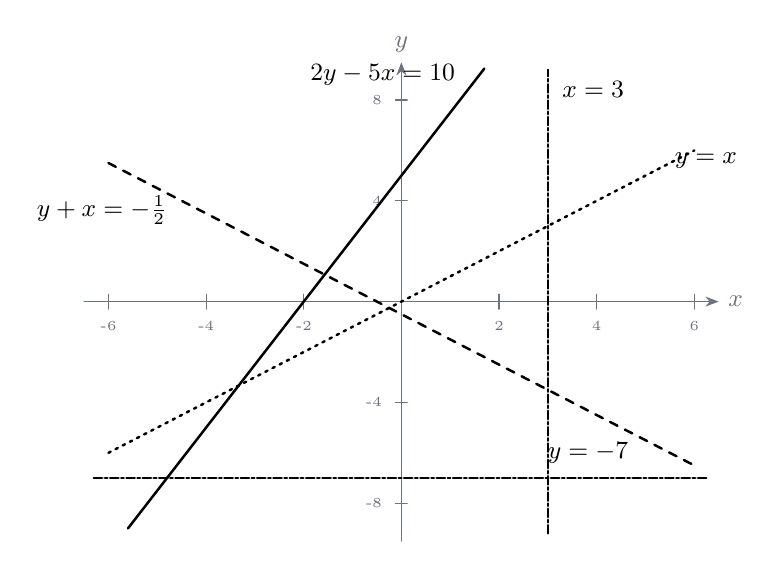
\begin{tikzpicture}[xscale=0.62,yscale=0.32]
\draw[-Stealth,gray](-6.5,0)--(6.5,0) node[right]{\small $x$};
\draw[-Stealth,gray](0,-9.5)--(0,9.5) node[above]{\small $y$};
\foreach \t in {-6,-4,-2,2,4,6}{\draw[gray](\t,-0.3)--(\t,0.3); \node[below,gray] at (\t,-0.4){\tiny \t};}
\foreach \t in {-8,-4,4,8}{\draw[gray](-0.12,\t)--(0.12,\t); \node[left,gray] at (-0.2,\t){\tiny \t};}
\draw[thick,domain=-5.6:1.7] plot(\x,{2.5*\x+5});
\node[above left] at (1.3,8.2){\small $2y-5x=10$};
\draw[thick,dashed,domain=-6:6] plot(\x,{-\x-0.5});
\node[below left] at (-4.6,4.6){\small $y+x=-\frac{1}{2}$};
\draw[thick,dotted,domain=-6:6] plot(\x,{\x});
\node[right] at (5.4,5.6){\small $y=x$};
\draw[thick,densely dashdotted] (-6.3,-7)--(6.3,-7);
\node[above right] at (2.8,-6.8){\small $y=-7$};
\draw[thick,densely dashdotted] (3,-9.2)--(3,9.2);
\node[right] at (3.1,8.4){\small $x=3$};
\end{tikzpicture}
\caption{The five lines. Note that $y=-7$ is horizontal and $x=3$ is vertical --- the variable that is \emph{absent} tells you which way the line runs.}
\end{figure}

\begin{note}
Parts (iv) and (v) are the ones that get swapped. The rule is that the line is
perpendicular to the axis of the variable that appears. In $y=-7$ only $y$ appears, so
the line is perpendicular to the $y$-axis, that is horizontal.
\end{note}
\end{solution}

\begin{problem}
Determine the nature of the roots of each equation.
\quad (i) $2x^2-2x-5=0$, \quad (ii) $6x^2+4x+2=0$, \quad (iii) $x^2-10x+25=0$, \quad
(iv) $x^2+3x=0$, \quad (v) $x^2-25=0$, \quad (vi) $x^2=0$.
\end{problem}

\begin{solution}
Everything is decided by the discriminant of $ax^2+bx+c=0$:
$$\Delta=b^2-4ac.$$
$$\Delta>0\ \implies\ \text{two distinct real roots},\qquad
\Delta=0\ \implies\ \text{one repeated real root},$$
$$\Delta<0\ \implies\ \text{no real roots (two complex roots)}.$$
When $\Delta>0$ there is a further distinction: if $\Delta$ is a perfect square the
roots are rational, otherwise irrational.

\begin{table}[H]
\centering
\begin{tabular}{|l|c|c|c|c|l|}
\hline
 & $a$ & $b$ & $c$ & $\Delta=b^2-4ac$ & Nature of the roots\\
\hline
(i) & 2 & $-2$ & $-5$ & $4+40=44$ & two distinct real, irrational\\
(ii) & 6 & 4 & 2 & $16-48=-32$ & no real roots; two complex\\
(iii) & 1 & $-10$ & 25 & $100-100=0$ & one repeated real root\\
(iv) & 1 & 3 & 0 & $9-0=9$ & two distinct real, rational\\
(v) & 1 & 0 & $-25$ & $0+100=100$ & two distinct real, rational\\
(vi) & 1 & 0 & 0 & $0-0=0$ & one repeated real root\\
\hline
\end{tabular}
\end{table}

The roots themselves, for confirmation:
$$\text{(i) } x=\frac{1\pm\sqrt{11}}{2},\qquad
\text{(iii) } x=5 \text{ twice},\qquad
\text{(iv) } x(x+3)=0\ \implies\ x=0,-3,$$
$$\text{(v) } x=\pm 5,\qquad \text{(vi) } x=0 \text{ twice}.$$

\begin{note}
In (iv) and (vi) a coefficient is zero, and it must still be substituted as zero rather
than ignored. Writing $\Delta=b^2-4ac$ with $c$ simply left out of (iv) gives $9-4=5$
instead of $9$, and although the conclusion happens to survive, the working does not.
\end{note}

\begin{note}
$\Delta=0$ is often read as ``only one root''. More precisely there are two roots that
have coincided: (iii) factorises as $(x-5)^2=0$ and (vi) as $x^2=0$. The graph touches
the $x$-axis at that point rather than crossing it, which is what a repeated root looks
like.
\end{note}
\end{solution}

\begin{problem}
Find the value(s) of $k$ for which the quadratic equation has equal roots.
\quad (i) $x^2+2kx+25=0$, \quad (ii) $kx^2+12x+k=0$.
\end{problem}

\begin{solution}
Equal roots means $\Delta=0$.

\textbf{(i).} Here $a=1$, $b=2k$, $c=25$:
$$\Delta=(2k)^2-4(1)(25)=4k^2-100=0$$
$$4k^2=100\quad\implies\quad k^2=25\quad\implies\quad k=\pm 5.$$

Checking: $k=5$ gives $x^2+10x+25=(x+5)^2$, and $k=-5$ gives $x^2-10x+25=(x-5)^2$. Both
are perfect squares. $\checkmark$

\textbf{(ii).} Here $a=k$, $b=12$, $c=k$:
$$\Delta=12^2-4(k)(k)=144-4k^2=0$$
$$4k^2=144\quad\implies\quad k^2=36\quad\implies\quad k=\pm 6.$$

\begin{note}
In (ii) the value $k=0$ has to be excluded separately, and not because of the
discriminant. If $k=0$ the equation collapses to $12x=0$, which is linear and has one
root rather than two equal ones --- it is not a quadratic at all. Here $k=0$ is not
among the answers anyway, but whenever the leading coefficient contains the unknown it
is worth a moment's thought.
\end{note}

\begin{note}
Both answers come in $\pm$ pairs because $k$ appears squared in the discriminant. Giving
only the positive value is a common way to lose half the marks.
\end{note}
\end{solution}

\begin{problem}
By completing the square, rewrite each function in the form $f(x)=a(x-h)^2+k$. Hence
sketch the graph, showing the $x$- and $y$-intercepts and the turning point, and state
the range.
\quad (i) $f(x)=-2x^2+4x-5$, \quad (ii) $f(x)=4-3x^2$, \quad
(iii) $f(x)=3x^2+6x-4$, \quad (iv) $f(x)=4x^2-12x+3$, \quad
(v) $f(x)=x^2+10x+25$, \quad (vi) $f(x)=x^2-12x+36$.
\end{problem}

\begin{solution}
In the form $a(x-h)^2+k$, the turning point is $(h,k)$, and the parabola opens upwards
if $a>0$ and downwards if $a<0$. The $y$-intercept is $f(0)$; the $x$-intercepts are
found by solving $f(x)=0$, and there may be none.

\textbf{(i).} Take the $-2$ out of the first two terms only:
$$-2x^2+4x-5=-2\left(x^2-2x\right)-5=-2\left[(x-1)^2-1\right]-5$$
$$=-2(x-1)^2+2-5=-2(x-1)^2-3.$$
Turning point $(1,-3)$, a \emph{maximum} since $a=-2<0$. $y$-intercept $f(0)=-5$.
For the $x$-intercepts, $-2(x-1)^2=3$ has no solution, since the left side is never
positive: \textbf{no $x$-intercepts}.
$$\text{range}=(-\infty,-3].$$

\textbf{(ii).} Already almost in the required form:
$$4-3x^2=-3(x-0)^2+4.$$
Turning point $(0,4)$, a maximum. $y$-intercept $4$. Setting $f(x)=0$:
$$3x^2=4\quad\implies\quad x=\pm\frac{2}{\sqrt{3}}=\pm\frac{2\sqrt{3}}{3}\approx\pm 1.15.$$
$$\text{range}=(-\infty,4].$$

\textbf{(iii).}
$$3x^2+6x-4=3\left(x^2+2x\right)-4=3\left[(x+1)^2-1\right]-4=3(x+1)^2-7.$$
Turning point $(-1,-7)$, a minimum. $y$-intercept $-4$. For the $x$-intercepts:
$$3(x+1)^2=7\quad\implies\quad (x+1)^2=\frac{7}{3}\quad\implies\quad
x=-1\pm\frac{\sqrt{21}}{3}\approx -2.53 \text{ and } 0.53.$$
$$\text{range}=[-7,\infty).$$

\textbf{(iv).}
$$4x^2-12x+3=4\left(x^2-3x\right)+3=4\left[\left(x-\tfrac{3}{2}\right)^2
-\tfrac{9}{4}\right]+3=4\left(x-\tfrac{3}{2}\right)^2-9+3
=4\left(x-\tfrac{3}{2}\right)^2-6.$$
Turning point $\left(\frac{3}{2},-6\right)$, a minimum. $y$-intercept $3$. Roots:
$$\left(x-\tfrac{3}{2}\right)^2=\tfrac{3}{2}\quad\implies\quad
x=\frac{3}{2}\pm\frac{\sqrt{6}}{2}\approx 0.27 \text{ and } 2.72.$$
$$\text{range}=[-6,\infty).$$

\textbf{(v).} This one is already a perfect square:
$$x^2+10x+25=(x+5)^2+0.$$
Turning point $(-5,0)$, a minimum sitting \emph{on} the $x$-axis. $y$-intercept $25$.
There is one $x$-intercept, $x=-5$, a repeated root where the curve touches the axis.
$$\text{range}=[0,\infty).$$

\textbf{(vi).} Likewise:
$$x^2-12x+36=(x-6)^2+0.$$
Turning point $(6,0)$, $y$-intercept $36$, one $x$-intercept at $x=6$ where the curve
touches.
$$\text{range}=[0,\infty).$$

\begin{figure}[H]
\centering
\begin{tikzpicture}[xscale=0.85,yscale=0.30]
\draw[-Stealth,gray](-4.3,0)--(4.3,0) node[right]{\small $x$};
\draw[-Stealth,gray](0,-9)--(0,7.5) node[above]{\small $y$};
\foreach \t in {-3,-2,-1,1,2,3}{\draw[gray](\t,-0.35)--(\t,0.35); \node[below,gray] at (\t,-0.5){\tiny \t};}
\foreach \t in {-8,-4,4}{\draw[gray](-0.07,\t)--(0.07,\t); \node[left,gray] at (-0.12,\t){\tiny \t};}
\draw[thick,domain=-1.15:3.15,samples=60] plot(\x,{-2*(\x-1)^2-3});
\fill (1,-3) circle[radius=2.2pt]; \node[above] at (1,-2.6){\tiny $(1,-3)$};
\node[right] at (3.05,-11.5){};
\node at (3.05,-6.4){\small (i)};
\draw[thick,dashed,domain=-2.1:2.1,samples=60] plot(\x,{3*(\x+1)^2-7});
\fill (-1,-7) circle[radius=2.2pt]; \node[below] at (-1,-7.4){\tiny $(-1,-7)$};
\node at (-2.35,3.2){\small (iii)};
\end{tikzpicture}
\caption{Two of the six: (i) opens downward and never reaches the $x$-axis; (iii) opens upward and crosses it twice.}
\end{figure}

\begin{figure}[H]
\centering
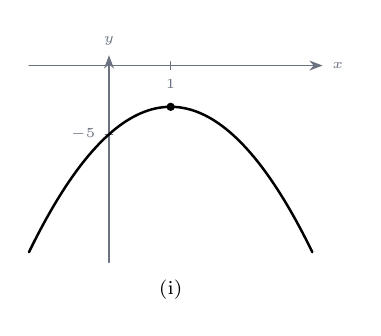
\begin{tikzpicture}
\draw[-Stealth,gray](0.000,2.500)--(3.730,2.500) node[right,font=\tiny]{$x$};
\draw[-Stealth,gray](1.017,0.000)--(1.017,2.630) node[above,font=\tiny]{$y$};
\draw[gray](1.800,2.450)--(1.800,2.550);
\node[below=0pt,gray,font=\tiny] at (1.800,2.450) {$1$};
\draw[gray](0.967,1.627)--(1.067,1.627);
\node[left=0pt,gray,font=\tiny] at (0.967,1.627) {$-5$};
\draw[thick,domain=-1.3:3.3,samples=120,variable=\t] plot({((\t)-(-1.3))/(4.6)*3.6},{((-2*\t*\t + 4*\t - 5)-(-14.321))/(14.321)*2.5});
\fill (1.800,1.976) circle[radius=1.5pt];
\node[font=\scriptsize] at (1.800,-0.340) {(i)};
\end{tikzpicture}
\hspace{0.35em}
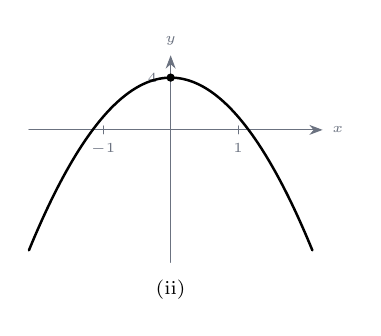
\begin{tikzpicture}
\draw[-Stealth,gray](0.000,1.683)--(3.730,1.683) node[right,font=\tiny]{$x$};
\draw[-Stealth,gray](1.800,0.000)--(1.800,2.630) node[above,font=\tiny]{$y$};
\draw[gray](0.943,1.633)--(0.943,1.733);
\node[below=0pt,gray,font=\tiny] at (0.943,1.633) {$-1$};
\draw[gray](2.657,1.633)--(2.657,1.733);
\node[below=0pt,gray,font=\tiny] at (2.657,1.633) {$1$};
\draw[gray](1.750,2.347)--(1.850,2.347);
\node[left=0pt,gray,font=\tiny] at (1.750,2.347) {$4$};
\draw[thick,domain=-2.1:2.1,samples=120,variable=\t] plot({((\t)-(-2.1))/(4.2)*3.6},{((4 - 3*\t*\t)-(-10.156))/(15.082)*2.5});
\fill (1.800,2.347) circle[radius=1.5pt];
\node[font=\scriptsize] at (1.800,-0.340) {(ii)};
\end{tikzpicture}
\hspace{0.35em}
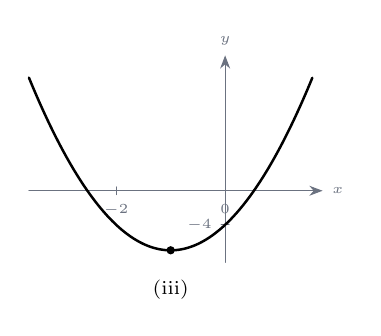
\begin{tikzpicture}
\draw[-Stealth,gray](0.000,0.910)--(3.730,0.910) node[right,font=\tiny]{$x$};
\draw[-Stealth,gray](2.492,0.000)--(2.492,2.630) node[above,font=\tiny]{$y$};
\draw[gray](1.108,0.860)--(1.108,0.960);
\node[below=0pt,gray,font=\tiny] at (1.108,0.860) {$-2$};
\draw[gray](2.492,0.860)--(2.492,0.960);
\node[below=0pt,gray,font=\tiny] at (2.492,0.860) {$0$};
\draw[gray](2.442,0.478)--(2.542,0.478);
\node[left=0pt,gray,font=\tiny] at (2.442,0.478) {$-4$};
\draw[thick,domain=-3.6:1.6,samples=120,variable=\t] plot({((\t)-(-3.6))/(5.2)*3.6},{((3*\t*\t + 6*\t - 4)-(-8.42))/(23.119999999999997)*2.5});
\fill (1.800,0.154) circle[radius=1.5pt];
\node[font=\scriptsize] at (1.800,-0.340) {(iii)};
\end{tikzpicture}

\vspace{1.4em}

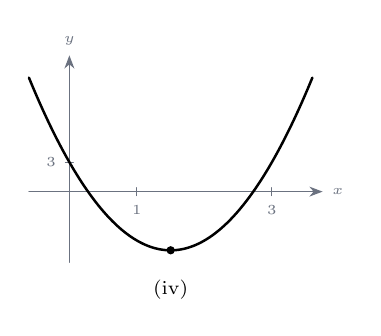
\begin{tikzpicture}
\draw[-Stealth,gray](0.000,0.899)--(3.730,0.899) node[right,font=\tiny]{$x$};
\draw[-Stealth,gray](0.514,0.000)--(0.514,2.630) node[above,font=\tiny]{$y$};
\draw[gray](1.371,0.849)--(1.371,0.949);
\node[below=0pt,gray,font=\tiny] at (1.371,0.849) {$1$};
\draw[gray](3.086,0.849)--(3.086,0.949);
\node[below=0pt,gray,font=\tiny] at (3.086,0.849) {$3$};
\draw[gray](0.464,1.272)--(0.564,1.272);
\node[left=0pt,gray,font=\tiny] at (0.464,1.272) {$3$};
\draw[thick,domain=-0.6:3.6,samples=120,variable=\t] plot({((\t)-(-0.6))/(4.2)*3.6},{((4*\t*\t - 12*\t + 3)-(-7.235))/(20.11)*2.5});
\fill (1.800,0.154) circle[radius=1.5pt];
\node[font=\scriptsize] at (1.800,-0.340) {(iv)};
\end{tikzpicture}
\hspace{0.35em}
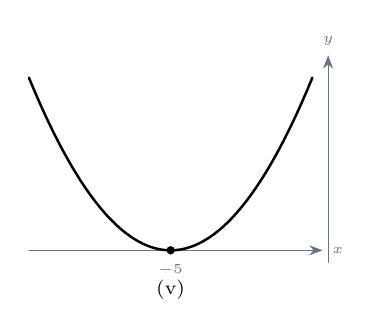
\begin{tikzpicture}
\draw[-Stealth,gray](0.000,0.154)--(3.730,0.154) node[right,font=\tiny]{$x$};
\draw[-Stealth,gray](3.800,0.000)--(3.800,2.630) node[above,font=\tiny]{$y$};
\draw[gray](1.800,0.104)--(1.800,0.204);
\node[below=0pt,gray,font=\tiny] at (1.800,0.104) {$-5$};
\draw[thick,domain=-9.5:-0.5,samples=120,variable=\t] plot({((\t)-(-9.5))/(9.0)*3.6},{((\t*\t + 10*\t + 25)-(-1.418))/(23.086)*2.5});
\fill (1.800,0.154) circle[radius=1.5pt];
\node[font=\scriptsize] at (1.800,-0.340) {(v)};
\end{tikzpicture}
\hspace{0.35em}
\begin{tikzpicture}
\draw[-Stealth,gray](0.000,0.154)--(3.730,0.154) node[right,font=\tiny]{$x$};
\draw[-Stealth,gray](-0.600,0.000)--(-0.600,2.630) node[above,font=\tiny]{$y$};
\draw[gray](1.800,0.104)--(1.800,0.204);
\node[below=0pt,gray,font=\tiny] at (1.800,0.104) {$6$};
\draw[thick,domain=1.5:10.5,samples=120,variable=\t] plot({((\t)-(1.5))/(9.0)*3.6},{((\t*\t - 12*\t + 36)-(-1.418))/(23.086)*2.5});
\fill (1.800,0.154) circle[radius=1.5pt];
\node[font=\scriptsize] at (1.800,-0.340) {(vi)};
\end{tikzpicture}
\caption{All six of question 2(b), each turning point marked. In (v) and (vi) the turning point sits on the axis, which is the repeated-root case.}
\end{figure}

\begin{note}
The single commonest error is losing the factor $a$ when it comes back out of the
bracket. In (iii) the $-1$ inside the bracket becomes $3\times(-1)=-3$ on the way out,
giving $-4-3=-7$ and not $-4-1=-5$. Multiplying out the finished form to check it agrees
with the original takes ten seconds and catches this every time.
\end{note}

\begin{note}
Parts (v) and (vi) have $k=0$, which is exactly the case $\Delta=0$ from the previous
question --- one repeated root, the curve touching the axis rather than crossing. The
two questions are describing the same thing from different directions.
\end{note}
\end{solution}

\begin{problem}
Sketch on the same axes, showing the $x$- and $y$-intercepts, the points of intersection
and the turning point:
\quad (i) $y=x^2-4x$ and $x+y=0$, \quad (ii) $y=3x^2-2x$ and $y=1-4x$, \quad
(iii) $y=x^2$ and $y=-x^2+6x$.
\end{problem}

\begin{solution}
To find where two curves meet, set their $y$-values equal and solve.

\textbf{(i).} The line is $y=-x$. Setting the two equal:
$$x^2-4x=-x\quad\implies\quad x^2-3x=0\quad\implies\quad x(x-3)=0,$$
so $x=0$ or $x=3$, giving the points $(0,0)$ and $(3,-3)$.

The parabola $y=x^2-4x=x(x-4)$ cuts the axis at $0$ and $4$, with turning point at
$x=2$, $y=-4$.

\textbf{(ii).} Setting the two equal:
$$3x^2-2x=1-4x\quad\implies\quad 3x^2+2x-1=0\quad\implies\quad (3x-1)(x+1)=0,$$
so $x=\frac{1}{3}$ or $x=-1$, giving the points $\left(\frac{1}{3},-\frac{1}{3}\right)$
and $(-1,5)$.

The parabola $y=x(3x-2)$ cuts the axis at $0$ and $\frac{2}{3}$, with turning point at
$x=\frac{1}{3}$, $y=-\frac{1}{3}$.

\textbf{(iii).} Setting the two equal:
$$x^2=-x^2+6x\quad\implies\quad 2x^2-6x=0\quad\implies\quad 2x(x-3)=0,$$
so $x=0$ or $x=3$, giving $(0,0)$ and $(3,9)$.

\begin{figure}[H]
\centering
\begin{tikzpicture}[xscale=0.95,yscale=0.30]
\draw[-Stealth,gray](-1.3,0)--(6.6,0) node[right]{\small $x$};
\draw[-Stealth,gray](0,-6)--(0,11) node[above]{\small $y$};
\foreach \t in {1,2,3,4,5,6}{\draw[gray](\t,-0.35)--(\t,0.35); \node[below,gray] at (\t,-0.5){\tiny \t};}
\foreach \t in {4,8}{\draw[gray](-0.07,\t)--(0.07,\t); \node[left,gray] at (-0.12,\t){\tiny \t};}
\draw[thick,domain=-0.8:3.3,samples=60] plot(\x,{\x*\x});
\node[left] at (3.1,10.3){\small $y=x^2$};
\draw[thick,dashed,domain=-0.4:6.4,samples=70] plot(\x,{-\x*\x+6*\x});
\node[right] at (5.4,3.4){\small $y=-x^2+6x$};
\fill (0,0) circle[radius=2.2pt]; \fill (3,9) circle[radius=2.2pt];
\node[right] at (3.15,9){\tiny $(3,9)$};
\end{tikzpicture}
\caption{Part (iii). The two parabolas meet at the origin and at $(3,9)$; the region they enclose is the one whose area was found in the integration chapter.}
\end{figure}

\begin{figure}[H]
\centering
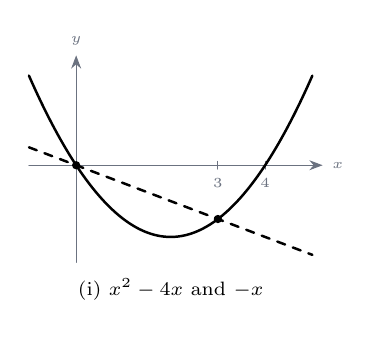
\begin{tikzpicture}
\draw[-Stealth,gray](0.000,1.234)--(3.730,1.234) node[right,font=\tiny]{$x$};
\draw[-Stealth,gray](0.600,0.000)--(0.600,2.630) node[above,font=\tiny]{$y$};
\draw[gray](2.400,1.184)--(2.400,1.284);
\node[below=0pt,gray,font=\tiny] at (2.400,1.184) {$3$};
\draw[gray](3.000,1.184)--(3.000,1.284);
\node[below=0pt,gray,font=\tiny] at (3.000,1.184) {$4$};
\draw[thick,domain=-1.0:5.0,samples=120,variable=\t] plot({((\t)-(-1.0))/(6.0)*3.6},{((\t*\t - 4*\t)-(-5.42))/(10.979)*2.5});
\draw[thick,dashed,domain=-1.0:5.0,samples=120,variable=\t] plot({((\t)-(-1.0))/(6.0)*3.6},{((-\t)-(-5.42))/(10.979)*2.5});
\fill (0.600,1.234) circle[radius=1.5pt];
\fill (2.400,0.551) circle[radius=1.5pt];
\node[font=\scriptsize] at (1.800,-0.340) {(i) $x^2-4x$ and $-x$};
\end{tikzpicture}
\hspace{0.35em}
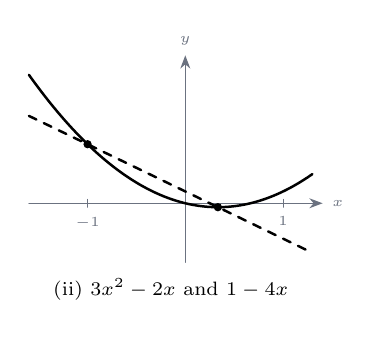
\begin{tikzpicture}
\draw[-Stealth,gray](0.000,0.751)--(3.730,0.751) node[right,font=\tiny]{$x$};
\draw[-Stealth,gray](1.986,0.000)--(1.986,2.630) node[above,font=\tiny]{$y$};
\draw[gray](0.745,0.701)--(0.745,0.801);
\node[below=0pt,gray,font=\tiny] at (0.745,0.701) {$-1$};
\draw[gray](3.228,0.701)--(3.228,0.801);
\node[below=0pt,gray,font=\tiny] at (3.228,0.701) {$1$};
\draw[thick,domain=-1.6:1.3,samples=120,variable=\t] plot({((\t)-(-1.6))/(2.9000000000000004)*3.6},{((3*\t*\t - 2*\t)-(-5.012))/(16.677)*2.5});
\draw[thick,dashed,domain=-1.6:1.3,samples=120,variable=\t] plot({((\t)-(-1.6))/(2.9000000000000004)*3.6},{((1 - 4*\t)-(-5.012))/(16.677)*2.5});
\fill (0.745,1.501) circle[radius=1.5pt];
\fill (2.400,0.701) circle[radius=1.5pt];
\node[font=\scriptsize] at (1.800,-0.340) {(ii) $3x^2-2x$ and $1-4x$};
\end{tikzpicture}
\caption{The remaining two pairs of question 2(c), curve solid and line dashed, with the points of intersection marked.}
\end{figure}

\begin{note}
Always simplify to ``$=0$'' before solving, as in every part above. Trying to cancel an
$x$ from $x^2-4x=-x$ to get $x-4=-1$ loses the root $x=0$ entirely --- dividing by $x$
is only legitimate when $x\neq 0$, and here it is one of the answers.
\end{note}
\end{solution}

\begin{problem}
The number of \emph{Vibrio cholerae} in refrigerated water is
$$N(T)=20T^2-20T+120,\qquad -2\leq T\leq 14,$$
where $T$ is the temperature in degrees Celsius.
\begin{enumerate}
\item[(a).] Find the number of bacteria at $0^\circ$.
\item[(b).] Find the number of bacteria at $10^\circ$.
\item[(c).] At what temperature is the number of bacteria smallest?
\end{enumerate}
\end{problem}

\begin{solution}
\textbf{(a).} Substitute $T=0$:
$$N(0)=20(0)-20(0)+120=120\ \text{bacteria}.$$

\textbf{(b).} Substitute $T=10$:
$$N(10)=20(100)-20(10)+120=2000-200+120=1920\ \text{bacteria}.$$

\textbf{(c).} The coefficient of $T^2$ is positive, so the parabola opens upwards and
its turning point is a minimum. Completing the square:
$$20T^2-20T+120=20\left(T^2-T\right)+120
=20\left[\left(T-\tfrac{1}{2}\right)^2-\tfrac{1}{4}\right]+120$$
$$=20\left(T-\tfrac{1}{2}\right)^2-5+120=20\left(T-\tfrac{1}{2}\right)^2+115.$$
The square is smallest when it is zero, at $T=\frac{1}{2}$.

$$\therefore\quad \text{the number is smallest at } T=0.5^\circ\text{C},
\text{ where } N=115 \text{ bacteria}.$$

\begin{note}
The answer $T=\frac{1}{2}$ lies inside the stated range $-2\leq T\leq 14$, so it is
genuinely the minimum. Had the turning point fallen outside the range, the smallest
value would have occurred at whichever endpoint was nearer, and the vertex would have
been the wrong answer. Always check the turning point against the domain the question
gives.
\end{note}
\end{solution}

\begin{problem}
The daily profit in dollars of a small company is
$$f(x)=-16x^2+64x+190,$$
where $x$ is the number of products sold each day. Find the number sold that maximises
the profit, and the maximum profit.
\end{problem}

\begin{solution}
The coefficient of $x^2$ is negative, so the parabola opens downwards and its turning
point is a maximum. Completing the square:
$$-16x^2+64x+190=-16\left(x^2-4x\right)+190
=-16\left[(x-2)^2-4\right]+190$$
$$=-16(x-2)^2+64+190=-16(x-2)^2+254.$$

The largest value occurs when the square is zero, at $x=2$:
$$\therefore\quad \text{selling } 2 \text{ products a day gives a maximum profit of
\$}254.$$

\begin{note}
The $y$-intercept is $f(0)=190$, the profit from selling nothing. That is not
nonsense here --- it just means the model is a rough one, since a real business selling
nothing would not make \$190. Reading off what a model says at the edges of its range is
a good habit, and a good way to notice its limits.
\end{note}
\end{solution}

\begin{problem}
The length of a rectangular fence is three more than twice the width. Determine the
dimensions that give a total area of $27\text{ m}^2$.
\end{problem}

\begin{solution}
\textbf{Step 1 --- name the unknown.} Let the width be $w$ metres. Then the length is
$$\ell=2w+3.$$

\textbf{Step 2 --- form the equation.}
$$\text{area}=w\ell=w(2w+3)=27.$$

\textbf{Step 3 --- rearrange and solve.}
$$2w^2+3w-27=0.$$
Factorising --- looking for two numbers multiplying to $2\times(-27)=-54$ and adding to
$3$, namely $9$ and $-6$:
$$2w^2+9w-6w-27=0$$
$$w(2w+9)-3(2w+9)=0$$
$$(w-3)(2w+9)=0,$$
$$\implies\quad w=3\quad\text{or}\quad w=-\frac{9}{2}.$$

\textbf{Step 4 --- reject the impossible root.} A width cannot be negative, so
$w=-\frac{9}{2}$ is discarded and $w=3$.

$$\ell=2(3)+3=9.$$

$$\therefore\quad \text{the fence is } 3\text{ m by } 9\text{ m}.$$

\textbf{Check.} $3\times 9=27$~m$^2$. $\checkmark$

\begin{note}
Step 4 is part of the answer, not an afterthought. A quadratic from a word problem
almost always produces one root that the situation forbids, and saying explicitly why it
is rejected is what turns algebra into a solution.
\end{note}
\end{solution}

\begin{problem}
Use \textbf{long division} to divide each polynomial by the given divisor, and write it
in the form $f(x)=Q(x)D(x)+R(x)$.
\begin{enumerate}
\item[(i).] $f(x)=x^2+3x+5$ by $x+1$
\item[(ii).] $f(x)=6x^3-19x^2+16x-4$ by $x-2$
\item[(iii).] $f(x)=x^3+6x^2-x+3$ by $2x^2-1$
\item[(iv).] $f(x)=x^4+3x^2+1$ by $x^2+2x+3$
\end{enumerate}
\end{problem}

\begin{solution}
\textbf{(i).} Dividing $x^2+3x+5$ by $x+1$:
$$x^2\div x=x;\quad x(x+1)=x^2+x;\quad \text{subtract: } 2x+5.$$
$$2x\div x=2;\quad 2(x+1)=2x+2;\quad \text{subtract: } 3.$$
$$\therefore\quad x^2+3x+5=(x+2)(x+1)+3.$$

\textbf{(ii).} Dividing $6x^3-19x^2+16x-4$ by $x-2$:
$$6x^3\div x=6x^2;\quad 6x^2(x-2)=6x^3-12x^2;\quad \text{subtract: } -7x^2+16x-4.$$
$$-7x^2\div x=-7x;\quad -7x(x-2)=-7x^2+14x;\quad \text{subtract: } 2x-4.$$
$$2x\div x=2;\quad 2(x-2)=2x-4;\quad \text{subtract: } 0.$$
$$\therefore\quad 6x^3-19x^2+16x-4=\left(6x^2-7x+2\right)(x-2)+0.$$
The remainder is zero, so $x-2$ is a factor.

\textbf{(iii).} Here the divisor $2x^2-1$ has degree $2$, so the quotient has degree
$3-2=1$ and the remainder degree at most $1$. Note that $2x^2-1$ has no $x$ term, which
must be treated as $0x$:
$$x^3\div 2x^2=\tfrac{1}{2}x;\quad \tfrac{1}{2}x\left(2x^2-1\right)=x^3-\tfrac{1}{2}x;
\quad \text{subtract: } 6x^2-\tfrac{1}{2}x+3.$$
$$6x^2\div 2x^2=3;\quad 3\left(2x^2-1\right)=6x^2-3;\quad
\text{subtract: } -\tfrac{1}{2}x+6.$$
$$\therefore\quad x^3+6x^2-x+3=\left(\tfrac{1}{2}x+3\right)\left(2x^2-1\right)
+\left(6-\tfrac{1}{2}x\right).$$

\textbf{(iv).} The dividend has no $x^3$ or $x$ term, so write it as
$x^4+0x^3+3x^2+0x+1$:
$$x^4\div x^2=x^2;\quad x^2\left(x^2+2x+3\right)=x^4+2x^3+3x^2;\quad
\text{subtract: } -2x^3+0x^2+0x+1.$$
$$-2x^3\div x^2=-2x;\quad -2x\left(x^2+2x+3\right)=-2x^3-4x^2-6x;\quad
\text{subtract: } 4x^2+6x+1.$$
$$4x^2\div x^2=4;\quad 4\left(x^2+2x+3\right)=4x^2+8x+12;\quad
\text{subtract: } -2x-11.$$
$$\therefore\quad x^4+3x^2+1=\left(x^2-2x+4\right)\left(x^2+2x+3\right)+(-2x-11).$$

\begin{note}
Missing powers must be written in as zeros, as in (iv). Skipping them causes terms to be
subtracted from the wrong column, and the answer comes out wrong without anything
looking obviously amiss.
\end{note}

\begin{note}
Part (iii) produces a fractional quotient, $\frac{1}{2}x+3$. That is perfectly
legitimate --- the quotient need not have whole-number coefficients when the divisor's
leading coefficient is not $1$. The check is always the same: multiply
$Q(x)D(x)$, add $R(x)$, and confirm the original returns.
\end{note}
\end{solution}

\begin{problem}
Use \textbf{synthetic division} to divide each polynomial by the given divisor, writing
it as $p(x)=q(x)(x-a)+r$.
\begin{enumerate}
\item[(i).] $p(x)=x^3-7x^2-4x+28$ by $x+2$
\item[(ii).] $p(x)=5x^3-6x^2-28x-2$ by $x+2$
\item[(iii).] $p(x)=x^3-10x^2-31x-30$ by $x-3$
\item[(iv).] $p(x)=6x^3+x^2-21x-10$ by $2x+1$
\end{enumerate}
\end{problem}

\begin{solution}
Synthetic division works with the value of $a$ for which the divisor vanishes: bring
down the leading coefficient, multiply by $a$, add to the next coefficient, and repeat.
The last number is the remainder and the rest are the coefficients of $q(x)$.

\textbf{(i).} Divisor $x+2$, so $a=-2$:

\begin{table}[H]
\centering
\begin{tabular}{|c|r r r r|}
\hline
$a=-2$ & 1 & $-7$ & $-4$ & 28\\
       &   & $-2$ & 18 & $-28$\\
\hline
       & 1 & $-9$ & 14 & \textbf{0}\\
\hline
\end{tabular}
\end{table}

$$\therefore\quad x^3-7x^2-4x+28=\left(x^2-9x+14\right)(x+2)+0.$$
The remainder is zero, so $x+2$ is a factor. Note also
$x^2-9x+14=(x-2)(x-7)$.

\textbf{(ii).} Divisor $x+2$, so $a=-2$:

\begin{table}[H]
\centering
\begin{tabular}{|c|r r r r|}
\hline
$a=-2$ & 5 & $-6$ & $-28$ & $-2$\\
       &   & $-10$ & 32 & $-8$\\
\hline
       & 5 & $-16$ & 4 & $\mathbf{-10}$\\
\hline
\end{tabular}
\end{table}

$$\therefore\quad 5x^3-6x^2-28x-2=\left(5x^2-16x+4\right)(x+2)-10.$$

\textbf{(iii).} Divisor $x-3$, so $a=3$:

\begin{table}[H]
\centering
\begin{tabular}{|c|r r r r|}
\hline
$a=3$ & 1 & $-10$ & $-31$ & $-30$\\
      &   & 3 & $-21$ & $-156$\\
\hline
      & 1 & $-7$ & $-52$ & $\mathbf{-186}$\\
\hline
\end{tabular}
\end{table}

$$\therefore\quad x^3-10x^2-31x-30=\left(x^2-7x-52\right)(x-3)-186.$$

\textbf{(iv).} The divisor is $2x+1$, not of the form $x-a$. It vanishes at
$x=-\frac{1}{2}$, so divide by $x+\frac{1}{2}$ first and adjust afterwards:

\begin{table}[H]
\centering
\begin{tabular}{|c|r r r r|}
\hline
$a=-\frac{1}{2}$ & 6 & 1 & $-21$ & $-10$\\
                 &   & $-3$ & 1 & 10\\
\hline
                 & 6 & $-2$ & $-20$ & \textbf{0}\\
\hline
\end{tabular}
\end{table}

$$6x^3+x^2-21x-10=\left(6x^2-2x-20\right)\left(x+\tfrac{1}{2}\right)+0.$$
Since $x+\frac{1}{2}=\frac{1}{2}(2x+1)$, move the factor of $\frac{1}{2}$ into the
quotient:
$$=\left(3x^2-x-10\right)(2x+1)+0.$$

\begin{note}
Part (iv) is the one to be careful with. Synthetic division always divides by
$x-a$, so with a divisor of $2x+1$ the quotient comes out twice as large as it should
and must be halved. Forgetting the adjustment gives a quotient that fails the
multiply-back check.
\end{note}

\begin{note}
The remainders here are $0$, $-10$, $-186$ and $0$, and each equals $p(a)$: for
instance in (ii), $p(-2)=-40-24+56-2=-10$. That is the remainder theorem, and it
gives a free check on every synthetic division.
\end{note}
\end{solution}

\begin{problem}
Factorise completely.
\quad (i) $4x^3-8x^2-x+2$, \quad (ii) $2x^3+3x^2-3x-2$, \quad
(iii) $x^3-2x^2+2x-4$, \quad (iv) $x^3-1$, \quad (v) $x^3+1$, \quad
(vi) $x^4-6x^3-11x^2+24x-28$.
\end{problem}

\begin{solution}
\textbf{(i).} Four terms with a common pattern --- group them:
$$4x^3-8x^2-x+2=4x^2(x-2)-1(x-2)=\left(4x^2-1\right)(x-2).$$
The first bracket is a difference of two squares:
$$=(2x-1)(2x+1)(x-2).$$

\textbf{(ii).} Try small values to find a root. $f(1)=2+3-3-2=0$, so $x-1$ is a factor.
Dividing:
$$2x^3+3x^2-3x-2=(x-1)\left(2x^2+5x+2\right)=(x-1)(2x+1)(x+2).$$

\textbf{(iii).} Group again:
$$x^3-2x^2+2x-4=x^2(x-2)+2(x-2)=\left(x^2+2\right)(x-2).$$
The bracket $x^2+2$ has no real roots, so this is as far as the factorisation goes over
the real numbers.

\textbf{(iv).} A difference of two cubes, $a^3-b^3=(a-b)\left(a^2+ab+b^2\right)$:
$$x^3-1=(x-1)\left(x^2+x+1\right).$$
The quadratic has $\Delta=1-4=-3<0$, so it does not factorise further over $\mathbb{R}$.

\textbf{(v).} A sum of two cubes, $a^3+b^3=(a+b)\left(a^2-ab+b^2\right)$:
$$x^3+1=(x+1)\left(x^2-x+1\right),$$
and again $\Delta=1-4=-3<0$.

\textbf{(vi).} As printed, this polynomial does not factorise. The rational root theorem
says any rational root must divide $28$, and testing every candidate
$\pm 1,\pm 2,\pm 4,\pm 7,\pm 14,\pm 28$ gives no zero --- for instance $f(1)=-20$,
$f(2)=-56$, $f(7)=-56$, $f(-2)=-56$.

Compare it with question 7(e) on the same sheet, which asks for the roots of
$$x^4-6x^3=11x^2-24x-28,\qquad\text{that is}\qquad x^4-6x^3-11x^2+24x+28=0.$$
That is the same polynomial with $+28$ in place of $-28$, and it factorises perfectly.
So the sign here is a misprint. Working with $+28$:

Testing candidates: $f(-1)=1+6-11-24+28=0$, so $x+1$ is a factor. Dividing,
$$x^4-6x^3-11x^2+24x+28=(x+1)\left(x^3-7x^2-4x+28\right),$$
and the cubic is the very one from question 6(b)(i), already factorised there as
$(x+2)\left(x^2-9x+14\right)=(x+2)(x-2)(x-7)$. Hence
$$x^4-6x^3-11x^2+24x+28=(x+1)(x+2)(x-2)(x-7).$$

\begin{note}
Parts (i) and (iii) are done by grouping and (ii) by the factor theorem. Grouping is
worth trying first on a four-term polynomial: it is quicker, and it either works
immediately or plainly does not.
\end{note}

\begin{note}
``Factorise completely'' means over the real numbers unless told otherwise, so
$x^2+2$, $x^2+x+1$ and $x^2-x+1$ are all left alone. Checking the discriminant is
negative is what justifies stopping.
\end{note}
\end{solution}

\begin{problem}
Solve each equation.
\quad (a) $x^3+x^2-x-1=0$, \quad (b) $2x^3+3x^2-3x=2$, \quad
(c) $x^3+6x^2+5x-2=0$, \quad (d) $x^2(2x+1)=13x-6$, \quad
(e) $x^4-6x^3=11x^2-24x-28$.
\end{problem}

\begin{solution}
\textbf{(a).} Group:
$$x^3+x^2-x-1=x^2(x+1)-1(x+1)=\left(x^2-1\right)(x+1)=(x-1)(x+1)^2=0.$$
$$\therefore\quad x=1\quad\text{or}\quad x=-1 \text{ (a repeated root)}.$$

\textbf{(b).} Move everything to one side:
$$2x^3+3x^2-3x-2=0,$$
which is question 6(c)(ii), already factorised as $(x-1)(2x+1)(x+2)$:
$$\therefore\quad x=1,\quad x=-\tfrac{1}{2},\quad x=-2.$$

\textbf{(c).} By the rational root theorem, any rational root must divide $2$, so the
candidates are $\pm 1$ and $\pm 2$:
$$f(1)=1+6+5-2=10,\qquad f(-1)=-1+6-5-2=-2,$$
$$f(2)=8+24+10-2=40,\qquad f(-2)=-8+24-10-2=4.$$
None is zero, so the equation has \emph{no rational roots} and cannot be solved by the
factor theorem, which is the only method available in this course. It does have three
irrational real roots, at approximately $-4.90$, $-1.40$ and $0.29$, but reaching them
needs either a numerical method or the cubic formula.

This is almost certainly a misprint for
$$x^3+6x^2+5x-12=0,$$
where the candidates dividing $12$ include $x=1$: $1+6+5-12=0$. Then
$$x^3+6x^2+5x-12=(x-1)\left(x^2+7x+12\right)=(x-1)(x+3)(x+4)=0,$$
$$\therefore\quad x=1,\quad x=-3,\quad x=-4.$$

\textbf{(d).} Expand and collect:
$$2x^3+x^2=13x-6\quad\implies\quad 2x^3+x^2-13x+6=0.$$
Candidates divide $6$. Testing $x=2$: $16+4-26+6=0$, so $x-2$ is a factor. Dividing,
$$2x^3+x^2-13x+6=(x-2)\left(2x^2+5x-3\right)=(x-2)(2x-1)(x+3)=0.$$
$$\therefore\quad x=2,\quad x=\tfrac{1}{2},\quad x=-3.$$

\textbf{(e).} Collect everything on the left:
$$x^4-6x^3-11x^2+24x+28=0,$$
which is the polynomial factorised in question 6(c)(vi):
$$(x+1)(x+2)(x-2)(x-7)=0,$$
$$\therefore\quad x=-1,\quad x=-2,\quad x=2,\quad x=7.$$

\begin{note}
Part (a) has a repeated root at $x=-1$, from the factor $(x+1)^2$. The equation has
three roots counted with repetition but only two distinct values, and the graph touches
the axis at $-1$ while crossing it at $1$.
\end{note}

\begin{note}
Every one of these must be rearranged to ``$=0$'' before the factor theorem can be used
at all. In (b) and (d) the equation is not presented that way, and testing values in the
un-rearranged form gives nothing useful.
\end{note}
\end{solution}

\begin{problem}
\begin{enumerate}
\item[(a).] Given that $x-1$ and $x+1$ are factors of $f(x)=ax^3+bx^2-3x-7$, find $a$
and $b$.
\item[(b).] Let $f(x)=x^3+ax^2+bx+6$. Given that the remainders when $f(x)$ is divided
by $x+1$ and $x-2$ are $20$ and $8$ respectively, find $a$ and $b$.
\end{enumerate}
\end{problem}

\begin{solution}
\textbf{(a).} If $x-1$ is a factor then $f(1)=0$, and if $x+1$ is a factor then
$f(-1)=0$.
$$f(1)=a+b-3-7=0\quad\implies\quad a+b=10,$$
$$f(-1)=-a+b+3-7=0\quad\implies\quad -a+b=4.$$
Adding the two equations eliminates $a$:
$$2b=14\quad\implies\quad b=7,$$
and then $a=10-7=3$.

$$\therefore\quad a=3,\ b=7.$$

\textbf{Check.} $f(x)=3x^3+7x^2-3x-7$. Then $f(1)=3+7-3-7=0$ and
$f(-1)=-3+7+3-7=0$. $\checkmark$

\textbf{(b).} By the remainder theorem, the remainder on dividing by $x-a$ is $f(a)$.
Dividing by $x+1$ means $a=-1$, and by $x-2$ means $a=2$:
$$f(-1)=-1+a-b+6=20\quad\implies\quad a-b=15,$$
$$f(2)=8+4a+2b+6=8\quad\implies\quad 4a+2b=-6\quad\implies\quad 2a+b=-3.$$
Adding the two equations eliminates $b$:
$$3a=12\quad\implies\quad a=4,$$
and then $b=a-15=4-15=-11$.

$$\therefore\quad a=4,\ b=-11.$$

\textbf{Check.} $f(x)=x^3+4x^2-11x+6$. Then
$$f(-1)=-1+4+11+6=20,\qquad f(2)=8+16-22+6=8.\ \checkmark$$

\begin{note}
``Factor'' and ``remainder'' are the same theorem. A factor is simply the case where
the remainder is zero, which is why (a) and (b) are solved by exactly the same two
steps: substitute the value that makes the divisor vanish, and equate to what the
question says the answer is.
\end{note}

\begin{note}
The sign is the trap. Dividing by $x+1$ means substituting $x=-1$, not $x=1$. Writing
the divisor as $x-(-1)$ before substituting removes the doubt.
\end{note}
\end{solution}

\begin{problem}
Sketch each function, clearly indicating the $x$- and $y$-intercepts.
\quad (a) $f(x)=x^3$, \quad (b) $f(x)=x^3+2$, \quad (c) $f(x)=15+5x-3x^2-x^3$, \quad
(d) $f(x)=x^3-4x^2+x+6$, \quad (e) $f(x)=4x^3-12x^2+5x+6$, \quad
(f) $f(x)=x^3-6x-5$.
\end{problem}

\begin{solution}
For a cubic sketch, three things are needed: the $y$-intercept $f(0)$, the
$x$-intercepts from factorising, and the direction the ends go. If the coefficient of
$x^3$ is positive the curve rises to the right and falls to the left; if negative, the
other way round.

\textbf{(a).} $f(x)=x^3$. Both intercepts are at the origin, a triple root, so the curve
flattens there and passes straight through. Positive leading coefficient.

\textbf{(b).} $f(x)=x^3+2$: the same curve lifted two units. $y$-intercept $2$, and the
single $x$-intercept where $x^3=-2$, that is $x=-\sqrt[3]{2}\approx-1.26$.

\textbf{(c).} $y$-intercept $15$. Factorising by grouping:
$$15+5x-3x^2-x^3=5(3+x)-x^2(3+x)=\left(5-x^2\right)(x+3).$$
$$\therefore\quad x=-3,\quad x=\pm\sqrt{5}\approx\pm 2.24.$$
The leading term is $-x^3$, so the curve falls to the right.

\textbf{(d).} $y$-intercept $6$. Testing candidates dividing $6$: $f(-1)=-1-4-1+6=0$,
so $x+1$ is a factor. Dividing,
$$x^3-4x^2+x+6=(x+1)\left(x^2-5x+6\right)=(x+1)(x-2)(x-3),$$
$$\therefore\quad x=-1,\quad x=2,\quad x=3.$$

\textbf{(e).} $y$-intercept $6$. Testing $x=2$: $32-48+10+6=0$, so $x-2$ is a factor.
Dividing,
$$4x^3-12x^2+5x+6=(x-2)\left(4x^2-4x-3\right)=(x-2)(2x-3)(2x+1),$$
$$\therefore\quad x=2,\quad x=\tfrac{3}{2},\quad x=-\tfrac{1}{2}.$$

\textbf{(f).} $y$-intercept $-5$. Testing $x=-1$: $-1+6-5=0$, so $x+1$ is a factor.
Dividing,
$$x^3-6x-5=(x+1)\left(x^2-x-5\right).$$
The quadratic has $\Delta=1+20=21>0$, giving
$$x=\frac{1\pm\sqrt{21}}{2}\approx -1.79 \text{ and } 2.79,$$
so there are three $x$-intercepts: $-1.79$, $-1$ and $2.79$.

\begin{figure}[H]
\centering
\begin{tikzpicture}[xscale=1.05,yscale=0.30]
\draw[-Stealth,gray](-2,0)--(4.2,0) node[right]{\small $x$};
\draw[-Stealth,gray](0,-4)--(0,9) node[above]{\small $y$};
\foreach \t in {-1,1,2,3}{\draw[gray](\t,-0.35)--(\t,0.35); \node[below,gray] at (\t,-0.55){\tiny \t};}
\node[left,gray] at (-0.1,6){\tiny 6};
\draw[thick,domain=-1.45:3.55,samples=90] plot(\x,{\x*\x*\x-4*\x*\x+\x+6});
\foreach \p in {(-1,0),(2,0),(3,0),(0,6)}{\fill \p circle[radius=2.2pt];}
\node[above] at (-1,0.4){\tiny $-1$};
\end{tikzpicture}
\caption{Part (d), $f(x)=(x+1)(x-2)(x-3)$: three simple roots, so the curve crosses the axis at each, and a $y$-intercept of 6.}
\end{figure}

\begin{figure}[H]
\centering
\begin{tikzpicture}
\draw[-Stealth,gray](0.000,1.250)--(3.730,1.250) node[right,font=\tiny]{$x$};
\draw[-Stealth,gray](1.800,0.000)--(1.800,2.630) node[above,font=\tiny]{$y$};
\draw[gray](0.741,1.200)--(0.741,1.300);
\node[below=0pt,gray,font=\tiny] at (0.741,1.200) {$-1$};
\draw[gray](2.859,1.200)--(2.859,1.300);
\node[below=0pt,gray,font=\tiny] at (2.859,1.200) {$1$};
\draw[thick,domain=-1.7:1.7,samples=120,variable=\t] plot({((\t)-(-1.7))/(3.4)*3.6},{((\t*\t*\t)-(-5.601))/(11.202)*2.5});
\fill (1.800,1.250) circle[radius=1.5pt];
\node[font=\scriptsize] at (1.800,-0.340) {(a)};
\end{tikzpicture}
\hspace{0.35em}
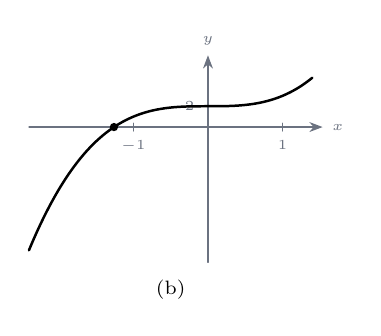
\begin{tikzpicture}
\draw[-Stealth,gray](0.000,1.719)--(3.730,1.719) node[right,font=\tiny]{$x$};
\draw[-Stealth,gray](2.274,0.000)--(2.274,2.630) node[above,font=\tiny]{$y$};
\draw[gray](1.326,1.669)--(1.326,1.769);
\node[below=0pt,gray,font=\tiny] at (1.326,1.669) {$-1$};
\draw[gray](3.221,1.669)--(3.221,1.769);
\node[below=0pt,gray,font=\tiny] at (3.221,1.669) {$1$};
\draw[gray](2.224,1.983)--(2.324,1.983);
\node[left=0pt,gray,font=\tiny] at (2.224,1.983) {$2$};
\draw[thick,domain=-2.4:1.4,samples=120,variable=\t] plot({((\t)-(-2.4))/(3.8)*3.6},{((\t*\t*\t + 2)-(-12.984))/(18.887999999999998)*2.5});
\fill (1.080,1.719) circle[radius=1.5pt];
\node[font=\scriptsize] at (1.800,-0.340) {(b)};
\end{tikzpicture}
\hspace{0.35em}
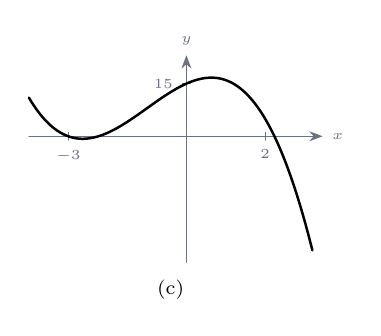
\begin{tikzpicture}
\draw[-Stealth,gray](0.000,1.602)--(3.730,1.602) node[right,font=\tiny]{$x$};
\draw[-Stealth,gray](2.000,0.000)--(2.000,2.630) node[above,font=\tiny]{$y$};
\draw[gray](0.500,1.552)--(0.500,1.652);
\node[below=0pt,gray,font=\tiny] at (0.500,1.552) {$-3$};
\draw[gray](3.000,1.552)--(3.000,1.652);
\node[below=0pt,gray,font=\tiny] at (3.000,1.552) {$2$};
\draw[gray](1.950,2.270)--(2.050,2.270);
\node[left=0pt,gray,font=\tiny] at (1.950,2.270) {$15$};
\draw[thick,domain=-4.0:3.2,samples=120,variable=\t] plot({((\t)-(-4.0))/(7.2)*3.6},{((-\t*\t*\t - 3*\t*\t + 5*\t + 15)-(-35.932))/(56.085)*2.5});
\node[font=\scriptsize] at (1.800,-0.340) {(c)};
\end{tikzpicture}

\vspace{1.4em}

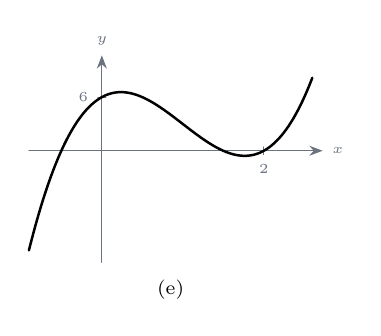
\begin{tikzpicture}
\draw[-Stealth,gray](0.000,1.418)--(3.730,1.418) node[right,font=\tiny]{$x$};
\draw[-Stealth,gray](0.926,0.000)--(0.926,2.630) node[above,font=\tiny]{$y$};
\draw[gray](2.983,1.368)--(2.983,1.468);
\node[below=0pt,gray,font=\tiny] at (2.983,1.368) {$2$};
\draw[gray](0.876,2.099)--(0.976,2.099);
\node[left=0pt,gray,font=\tiny] at (0.876,2.099) {$6$};
\draw[thick,domain=-0.9:2.6,samples=120,variable=\t] plot({((\t)-(-0.9))/(3.5)*3.6},{((4*\t*\t*\t - 12*\t*\t + 5*\t + 6)-(-12.488))/(22.024)*2.5});
\node[font=\scriptsize] at (1.800,-0.340) {(e)};
\end{tikzpicture}
\hspace{0.35em}
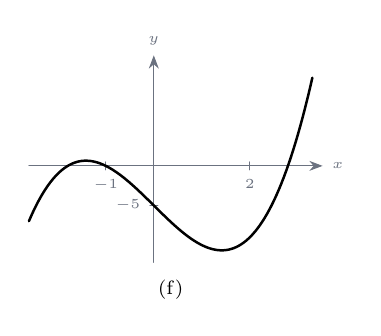
\begin{tikzpicture}
\draw[-Stealth,gray](0.000,1.226)--(3.730,1.226) node[right,font=\tiny]{$x$};
\draw[-Stealth,gray](1.586,0.000)--(1.586,2.630) node[above,font=\tiny]{$y$};
\draw[gray](0.976,1.176)--(0.976,1.276);
\node[below=0pt,gray,font=\tiny] at (0.976,1.176) {$-1$};
\draw[gray](2.807,1.176)--(2.807,1.276);
\node[below=0pt,gray,font=\tiny] at (2.807,1.176) {$2$};
\draw[gray](1.536,0.723)--(1.636,0.723);
\node[left=0pt,gray,font=\tiny] at (1.536,0.723) {$-5$};
\draw[thick,domain=-2.6:3.3,samples=120,variable=\t] plot({((\t)-(-2.6))/(5.9)*3.6},{((\t*\t*\t - 6*\t - 5)-(-12.182))/(24.845)*2.5});
\node[font=\scriptsize] at (1.800,-0.340) {(f)};
\end{tikzpicture}
\caption{The other five cubics of question 9. In (a) the triple root at the origin makes the curve flatten and pass straight through; in (c) the leading term is $-x^3$, so the curve falls to the right.}
\end{figure}

\begin{note}
The question asks only for the intercepts, not the turning points, and for these cubics
that is fortunate --- the turning points of (c), (d), (e) and (f) are all irrational. A
sketch showing the right roots, the right $y$-intercept and the right end behaviour is
what is wanted.
\end{note}

\begin{note}
Three distinct roots means the curve crosses the axis three times, as in (d) and (e). A
repeated root would make it touch instead, and a triple root, as in (a), makes it
flatten and pass through. Reading the multiplicity off the factorised form tells you the
shape at each intercept without any further work.
\end{note}
\end{solution}

\begin{note}
Question 2(a) on the printed sheet reads ``Solve the following using completing the
square method'' followed by an empty item (i) --- the equations were left out. The
method itself is exercised thoroughly by question 2(b) above, where every part is
completed to the form $a(x-h)^2+k$.
\end{note}


\begin{problem}
For each rational function, state the domain and the range, and sketch the graph.
\quad (i) $f(x)=\frac{2-x}{x+4}$, \quad (ii) $f(x)=\frac{3x+6}{x-1}$, \quad
(iii) $f(x)=\frac{x+1}{x-1}$, \quad (iv) $f(x)=\frac{2x+5}{x-1}$.
\end{problem}

\begin{solution}
Each of these has a linear top and a linear bottom, so each has one vertical asymptote
where the denominator vanishes and one horizontal asymptote given by the ratio of the
leading coefficients. The domain excludes the vertical asymptote and the range excludes
the horizontal one.

\begin{table}[H]
\centering
\begin{tabular}{|l|c|c|c|c|c|c|}
\hline
 & Vertical & Horizontal & Domain & Range & $x$-int & $y$-int\\
\hline
(i) & $x=-4$ & $y=-1$ & $\mathbb{R}-\{-4\}$ & $\mathbb{R}-\{-1\}$ & $2$ & $\frac{1}{2}$\\
(ii) & $x=1$ & $y=3$ & $\mathbb{R}-\{1\}$ & $\mathbb{R}-\{3\}$ & $-2$ & $-6$\\
(iii) & $x=1$ & $y=1$ & $\mathbb{R}-\{1\}$ & $\mathbb{R}-\{1\}$ & $-1$ & $-1$\\
(iv) & $x=1$ & $y=2$ & $\mathbb{R}-\{1\}$ & $\mathbb{R}-\{2\}$ & $-\frac{5}{2}$ & $-5$\\
\hline
\end{tabular}
\end{table}

Taking (iii) as the worked case:

\textbf{Vertical asymptote.} The denominator $x-1$ is zero at $x=1$, and the numerator
$x+1$ is $2$ there, so the fraction blows up: $x=1$.

\textbf{Horizontal asymptote.} Divide top and bottom by $x$:
$$\frac{x+1}{x-1}=\frac{1+\frac{1}{x}}{1-\frac{1}{x}}\longrightarrow\frac{1}{1}=1
\quad\text{as } x\to\pm\infty.$$
So $y=1$.

\textbf{Intercepts.} $f(0)=\frac{1}{-1}=-1$, and $f(x)=0$ when $x+1=0$, at $x=-1$.

\textbf{Range.} Solving $y=\frac{x+1}{x-1}$ for $x$:
$$y(x-1)=x+1\ \implies\ yx-y=x+1\ \implies\ x(y-1)=y+1\ \implies\ x=\frac{y+1}{y-1},$$
which is defined for every $y$ except $y=1$. So the range is $\mathbb{R}-\{1\}$.

\begin{figure}[H]
\centering
\begin{tikzpicture}[xscale=0.72,yscale=0.42]
\draw[-Stealth,gray](-4.4,0)--(6.4,0) node[right]{\small $x$};
\draw[-Stealth,gray](0,-6.4)--(0,6.4) node[above]{\small $y$};
\draw[dashed,gray] (1,-6.2)--(1,6.2); \node[above right,gray] at (1,5.4){\tiny $x=1$};
\draw[dashed,gray] (-4.3,1)--(6.3,1); \node[above left,gray] at (6.2,1){\tiny $y=1$};
\draw[thick,domain=-4.2:0.72,samples=90] plot(\x,{(\x+1)/(\x-1)});
\draw[thick,domain=1.32:6.2,samples=90] plot(\x,{(\x+1)/(\x-1)});
\fill (-1,0) circle[radius=2.2pt]; \fill (0,-1) circle[radius=2.2pt];
\node[below left] at (-1,-0.15){\tiny $-1$};
\end{tikzpicture}
\caption{Part (iii), $f(x)=\frac{x+1}{x-1}$. The curve approaches $y=1$ far out in both directions and never touches $x=1$.}
\end{figure}

\begin{figure}[H]
\centering
\begin{tikzpicture}
\draw[-Stealth,gray](0.000,1.477)--(3.730,1.477) node[right,font=\tiny]{$x$};
\draw[-Stealth,gray](2.475,0.000)--(2.475,2.630) node[above,font=\tiny]{$y$};
\draw[gray](2.925,1.427)--(2.925,1.527);
\node[below=0pt,gray,font=\tiny] at (2.925,1.427) {$2$};
\draw[dashed,gray](1.575,0.000)--(1.575,2.500);
\node[above,gray,font=\tiny] at (1.575,2.500) {$x=-4$};
\draw[dashed,gray](0.000,1.250)--(3.600,1.250);
\node[right,gray,font=\tiny] at (3.600,1.250) {$y=-1$};
\draw[thick,domain=-11:-4.55,samples=160,variable=\t] plot({((\t)-(-11))/(16)*3.6},{(((2-\t)/(\t+4))-(-6.5))/(11.0)*2.5});
\draw[thick,domain=-3.45:5,samples=160,variable=\t] plot({((\t)-(-11))/(16)*3.6},{(((2-\t)/(\t+4))-(-6.5))/(11.0)*2.5});
\node[font=\scriptsize] at (1.800,-0.340) {(i) $\frac{2-x}{x+4}$};
\end{tikzpicture}
\hspace{0.35em}
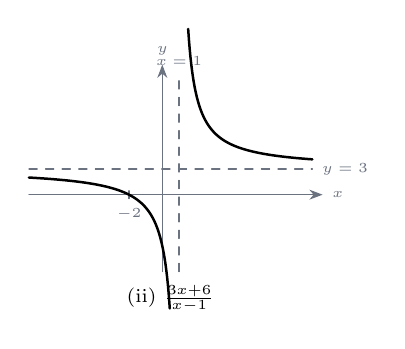
\begin{tikzpicture}
\draw[-Stealth,gray](0.000,0.978)--(3.730,0.978) node[right,font=\tiny]{$x$};
\draw[-Stealth,gray](1.694,0.000)--(1.694,2.630) node[above,font=\tiny]{$y$};
\draw[gray](1.271,0.928)--(1.271,1.028);
\node[below=0pt,gray,font=\tiny] at (1.271,0.928) {$-2$};
\draw[dashed,gray](1.906,0.000)--(1.906,2.500);
\node[above,gray,font=\tiny] at (1.906,2.500) {$x=1$};
\draw[dashed,gray](0.000,1.304)--(3.600,1.304);
\node[right,gray,font=\tiny] at (3.600,1.304) {$y=3$};
\draw[thick,domain=-8:0.44999999999999996,samples=160,variable=\t] plot({((\t)-(-8))/(17)*3.6},{(((3*\t+6)/(\t-1))-(-9))/(23)*2.5});
\draw[thick,domain=1.55:9,samples=160,variable=\t] plot({((\t)-(-8))/(17)*3.6},{(((3*\t+6)/(\t-1))-(-9))/(23)*2.5});
\node[font=\scriptsize] at (1.800,-0.340) {(ii) $\frac{3x+6}{x-1}$};
\end{tikzpicture}
\hspace{0.35em}
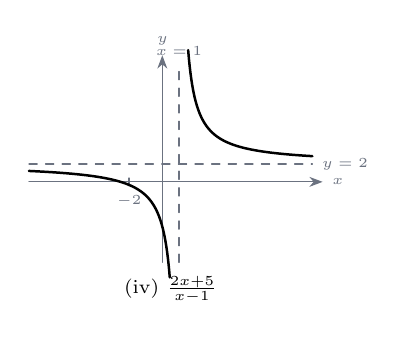
\begin{tikzpicture}
\draw[-Stealth,gray](0.000,1.023)--(3.730,1.023) node[right,font=\tiny]{$x$};
\draw[-Stealth,gray](1.694,0.000)--(1.694,2.630) node[above,font=\tiny]{$y$};
\draw[gray](1.271,0.973)--(1.271,1.073);
\node[below=0pt,gray,font=\tiny] at (1.271,0.973) {$-2$};
\draw[dashed,gray](1.906,0.000)--(1.906,2.500);
\node[above,gray,font=\tiny] at (1.906,2.500) {$x=1$};
\draw[dashed,gray](0.000,1.250)--(3.600,1.250);
\node[right,gray,font=\tiny] at (3.600,1.250) {$y=2$};
\draw[thick,domain=-8:0.44999999999999996,samples=160,variable=\t] plot({((\t)-(-8))/(17)*3.6},{(((2*\t+5)/(\t-1))-(-9))/(22)*2.5});
\draw[thick,domain=1.55:9,samples=160,variable=\t] plot({((\t)-(-8))/(17)*3.6},{(((2*\t+5)/(\t-1))-(-9))/(22)*2.5});
\node[font=\scriptsize] at (1.800,-0.340) {(iv) $\frac{2x+5}{x-1}$};
\end{tikzpicture}
\caption{The other three rational functions of question 1, with both asymptotes dashed. The curve approaches each without ever meeting it.}
\end{figure}

\begin{note}
The range is found by making $x$ the subject and asking which $y$ leave that formula
undefined. It is not a guess from the picture. In every case here the excluded value of
$y$ turns out to be the horizontal asymptote, which is what an asymptote means: a value
approached but never reached.
\end{note}

\begin{note}
In (ii) the horizontal asymptote is $y=3$, not $y=6$ or $y=0$. It is the ratio of the
coefficients of the highest power on each side, here $\frac{3x}{x}=3$; the constants
$+6$ and $-1$ become negligible as $x$ grows.
\end{note}
\end{solution}

\begin{problem}
Solve the following rational inequalities.
\quad (i) $\frac{2-x}{x+4}>0$, \quad (ii) $\frac{2x-3}{x-6}\geq x$, \quad
(iii) $\frac{8}{x+5}<4$, \quad (iv) $\frac{2x}{x-3}<4$.
\end{problem}

\begin{solution}
\begin{note}
Never multiply an inequality by a bracket containing $x$. The bracket may be negative,
which reverses the inequality sign, and there is no way to know which. Instead move
everything to one side, combine into a single fraction, and read the signs off a table.
\end{note}

\textbf{(i).} Already a single fraction. The critical values are where the numerator or
denominator vanishes: $x=2$ and $x=-4$.

\begin{table}[H]
\centering
\begin{tabular}{|l|c|c|c|}
\hline
 & $x<-4$ & $-4<x<2$ & $x>2$\\
\hline
$2-x$ & $+$ & $+$ & $-$\\
$x+4$ & $-$ & $+$ & $+$\\
quotient & $-$ & $+$ & $-$\\
\hline
\end{tabular}
\end{table}

$$\therefore\quad \frac{2-x}{x+4}>0 \text{ for } -4<x<2,\qquad\text{that is } (-4,2).$$

\textbf{(ii).} Move everything to one side:
$$\frac{2x-3}{x-6}-x\geq 0\quad\implies\quad \frac{(2x-3)-x(x-6)}{x-6}\geq 0
\quad\implies\quad \frac{-x^2+8x-3}{x-6}\geq 0.$$
Multiplying through by $-1$ reverses the sign:
$$\frac{x^2-8x+3}{x-6}\leq 0.$$
The numerator is zero when
$$x=\frac{8\pm\sqrt{64-12}}{2}=\frac{8\pm\sqrt{52}}{2}=4\pm\sqrt{13}
\approx 0.394 \text{ and } 7.606,$$
and the denominator at $x=6$.

\begin{table}[H]
\centering
\begin{tabular}{|l|c|c|c|c|}
\hline
 & $x<4-\sqrt{13}$ & $4-\sqrt{13}<x<6$ & $6<x<4+\sqrt{13}$ & $x>4+\sqrt{13}$\\
\hline
$x^2-8x+3$ & $+$ & $-$ & $-$ & $+$\\
$x-6$ & $-$ & $-$ & $+$ & $+$\\
quotient & $-$ & $+$ & $-$ & $+$\\
\hline
\end{tabular}
\end{table}

$$\therefore\quad x\leq 4-\sqrt{13}\quad\text{or}\quad 6<x\leq 4+\sqrt{13},$$
that is $\left(-\infty,\ 4-\sqrt{13}\right]\cup\left(6,\ 4+\sqrt{13}\right]$. The
endpoints from the numerator are included because the inequality is $\leq$; $x=6$ is
excluded because the expression is undefined there.

\textbf{(iii).}
$$\frac{8}{x+5}-4<0\quad\implies\quad \frac{8-4(x+5)}{x+5}<0
\quad\implies\quad \frac{-4x-12}{x+5}<0\quad\implies\quad \frac{-4(x+3)}{x+5}<0.$$
Dividing by $-4$ reverses the sign:
$$\frac{x+3}{x+5}>0.$$
Critical values $-5$ and $-3$; the quotient is positive outside them:
$$\therefore\quad x<-5\quad\text{or}\quad x>-3,\qquad
(-\infty,-5)\cup(-3,\infty).$$

\textbf{(iv).}
$$\frac{2x}{x-3}-4<0\quad\implies\quad \frac{2x-4(x-3)}{x-3}<0
\quad\implies\quad \frac{-2x+12}{x-3}<0\quad\implies\quad \frac{-2(x-6)}{x-3}<0.$$
Dividing by $-2$ and reversing:
$$\frac{x-6}{x-3}>0,$$
positive outside the critical values $3$ and $6$:
$$\therefore\quad x<3\quad\text{or}\quad x>6,\qquad (-\infty,3)\cup(6,\infty).$$

\begin{note}
Notice the answers to (iii) and (iv) are unions of two \emph{outer} pieces, with a gap
in the middle. Cross-multiplying $\frac{8}{x+5}<4$ to get $8<4x+20$ and hence
$x>-3$ finds only half the solution and misses everything below $-5$ entirely --- which
is exactly what the warning at the start is about.
\end{note}
\end{solution}

\begin{problem}
Solve each quadratic inequality, illustrating the solution set on a number line.
\quad (a) $2x^2+3x\geq 3$, \quad (b) $x^2-2x-3<0$, \quad (c) $x^2+2x\leq 8$, \quad
(d) $x^2-3x-4\neq 0$.
\end{problem}

\begin{solution}
\textbf{(a).} Move everything to one side: $2x^2+3x-3\geq 0$. The roots are
$$x=\frac{-3\pm\sqrt{9+24}}{4}=\frac{-3\pm\sqrt{33}}{4}\approx -2.19 \text{ and } 0.69.$$
The coefficient of $x^2$ is positive, so the parabola opens upwards and is
\emph{above} the axis outside its roots:
$$\therefore\quad x\leq\frac{-3-\sqrt{33}}{4}\quad\text{or}\quad
x\geq\frac{-3+\sqrt{33}}{4}.$$

\textbf{(b).} $x^2-2x-3=(x-3)(x+1)<0$. Roots $-1$ and $3$, parabola opening upwards, so
it is \emph{below} the axis between the roots:
$$\therefore\quad -1<x<3.$$

\textbf{(c).} $x^2+2x-8=(x+4)(x-2)\leq 0$. Roots $-4$ and $2$, below or on the axis
between them:
$$\therefore\quad -4\leq x\leq 2.$$

\textbf{(d).} This one is not really an inequality. $x^2-3x-4=(x-4)(x+1)$, which is zero
at $x=4$ and $x=-1$, so the expression is non-zero everywhere else:
$$\therefore\quad x\in\mathbb{R}-\{-1,4\}.$$

\begin{figure}[H]
\centering
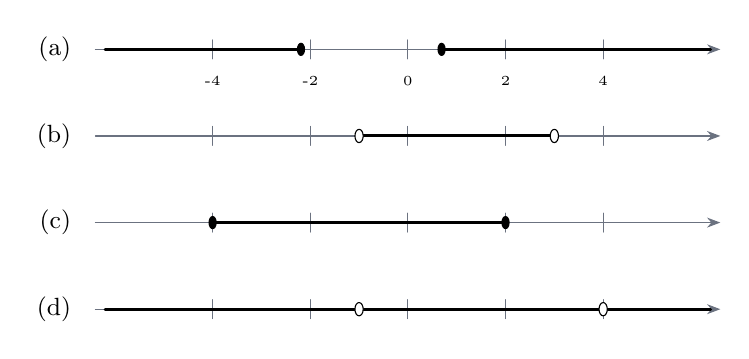
\begin{tikzpicture}[xscale=0.62,yscale=1]
\foreach \r/\lab in {0/{(a)}, 1/{(b)}, 2/{(c)}, 3/{(d)}}{
  \draw[-Stealth,gray] (-6.4,-1.1*\r)--(6.4,-1.1*\r);
  \node[left] at (-6.7,-1.1*\r) {\small \lab};
  \foreach \t in {-4,-2,0,2,4}{\draw[gray](\t,-1.1*\r-0.12)--(\t,-1.1*\r+0.12);}
}
\foreach \t in {-4,-2,0,2,4}{\node[below] at (\t,-0.22){\tiny \t};}
% (a)
\draw[very thick] (-6.2,0)--(-2.19,0); \fill (-2.19,0) circle(2.4pt);
\draw[very thick] (0.69,0)--(6.2,0); \fill (0.69,0) circle(2.4pt);
% (b)
\draw[very thick] (-1,-1.1)--(3,-1.1);
\draw[fill=white](-1,-1.1) circle(2.4pt); \draw[fill=white](3,-1.1) circle(2.4pt);
% (c)
\draw[very thick] (-4,-2.2)--(2,-2.2); \fill (-4,-2.2) circle(2.4pt); \fill (2,-2.2) circle(2.4pt);
% (d)
\draw[very thick] (-6.2,-3.3)--(6.2,-3.3);
\draw[fill=white](-1,-3.3) circle(2.4pt); \draw[fill=white](4,-3.3) circle(2.4pt);
\end{tikzpicture}
\caption{The four solution sets. Solid circles are included endpoints, hollow ones excluded.}
\end{figure}

\begin{note}
The shape of the answer follows from the direction the parabola opens. Upward-opening
and $\geq 0$ gives two outer pieces; upward-opening and $\leq 0$ gives one interval
between the roots. Sketching the parabola takes a moment and removes all doubt.
\end{note}
\end{solution}

\begin{problem}
Sketch each quadratic, and state the set of values of $x$ for which $f(x)>0$ and for
which $f(x)\leq 0$.
\quad (a) $f(x)=2x^2+3x-3$, \quad (b) $f(x)=-x^2-4x+1$, \quad
(c) $f(x)=2x^2-4x+5$, \quad (d) $f(x)=-2x^2-3x+2$.
\end{problem}

\begin{solution}
\textbf{(a).} $\Delta=9+24=33>0$, roots $\frac{-3\pm\sqrt{33}}{4}\approx -2.19$ and
$0.69$; opens upwards; $y$-intercept $-3$.
$$f(x)>0:\quad x<\tfrac{-3-\sqrt{33}}{4}\ \text{ or }\ x>\tfrac{-3+\sqrt{33}}{4},$$
$$f(x)\leq 0:\quad \tfrac{-3-\sqrt{33}}{4}\leq x\leq\tfrac{-3+\sqrt{33}}{4}.$$

\textbf{(b).} $\Delta=16+4=20>0$, roots $\frac{4\pm\sqrt{20}}{-2}=-2\pm\sqrt{5}\approx
-4.24$ and $0.24$; opens \emph{downwards}; $y$-intercept $1$. A downward parabola is
positive \emph{between} its roots:
$$f(x)>0:\quad -2-\sqrt{5}<x<-2+\sqrt{5},$$
$$f(x)\leq 0:\quad x\leq -2-\sqrt{5}\ \text{ or }\ x\geq -2+\sqrt{5}.$$

\textbf{(c).} $\Delta=16-40=-24<0$, so there are no real roots; opens upwards;
$y$-intercept $5$. The whole curve sits above the axis:
$$f(x)>0:\quad \text{all } x\in\mathbb{R},\qquad f(x)\leq 0:\quad \text{no values;
the empty set}.$$

\textbf{(d).} $\Delta=9+16=25$, a perfect square, so the roots are rational:
$$-2x^2-3x+2=-(2x^2+3x-2)=-(2x-1)(x+2),$$
giving $x=\frac{1}{2}$ and $x=-2$; opens downwards; $y$-intercept $2$:
$$f(x)>0:\quad -2<x<\tfrac{1}{2},\qquad
f(x)\leq 0:\quad x\leq -2\ \text{ or }\ x\geq\tfrac{1}{2}.$$

\begin{figure}[H]
\centering
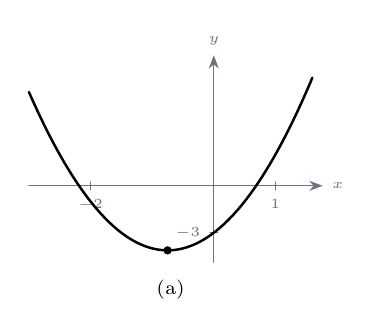
\begin{tikzpicture}
\draw[-Stealth,gray](0.000,0.973)--(3.730,0.973) node[right,font=\tiny]{$x$};
\draw[-Stealth,gray](2.348,0.000)--(2.348,2.630) node[above,font=\tiny]{$y$};
\draw[gray](0.783,0.923)--(0.783,1.023);
\node[below=0pt,gray,font=\tiny] at (0.783,0.923) {$-2$};
\draw[gray](3.130,0.923)--(3.130,1.023);
\node[below=0pt,gray,font=\tiny] at (3.130,0.923) {$1$};
\draw[gray](2.298,0.377)--(2.398,0.377);
\node[left=0pt,gray,font=\tiny] at (2.298,0.377) {$-3$};
\draw[thick,domain=-3.0:1.6,samples=120,variable=\t] plot({((\t)-(-3.0))/(4.6)*3.6},{((2*\t*\t + 3*\t - 3)-(-4.898))/(12.591)*2.5});
\fill (1.761,0.153) circle[radius=1.5pt];
\node[font=\scriptsize] at (1.800,-0.340) {(a)};
\end{tikzpicture}
\hspace{0.35em}
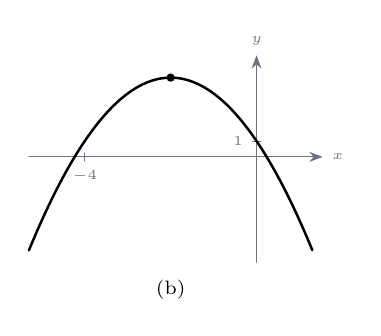
\begin{tikzpicture}
\draw[-Stealth,gray](0.000,1.340)--(3.730,1.340) node[right,font=\tiny]{$x$};
\draw[-Stealth,gray](2.891,0.000)--(2.891,2.630) node[above,font=\tiny]{$y$};
\draw[gray](0.709,1.290)--(0.709,1.390);
\node[below=0pt,gray,font=\tiny] at (0.709,1.290) {$-4$};
\draw[gray](2.841,1.541)--(2.941,1.541);
\node[left=0pt,gray,font=\tiny] at (2.841,1.541) {$1$};
\draw[thick,domain=-5.3:1.3,samples=120,variable=\t] plot({((\t)-(-5.3))/(6.6)*3.6},{((-\t*\t - 4*\t + 1)-(-6.652))/(12.414)*2.5});
\fill (1.800,2.347) circle[radius=1.5pt];
\node[font=\scriptsize] at (1.800,-0.340) {(b)};
\end{tikzpicture}

\vspace{1.4em}

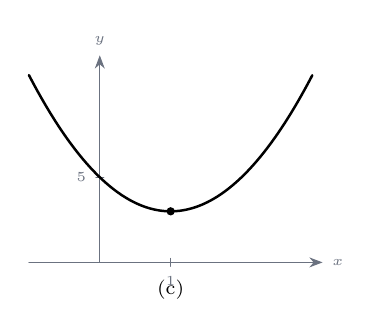
\begin{tikzpicture}
\draw[-Stealth,gray](0.000,0.000)--(3.730,0.000) node[right,font=\tiny]{$x$};
\draw[-Stealth,gray](0.900,0.000)--(0.900,2.630) node[above,font=\tiny]{$y$};
\draw[gray](1.800,-0.050)--(1.800,0.050);
\node[below=0pt,gray,font=\tiny] at (1.800,-0.050) {$1$};
\draw[gray](0.850,1.081)--(0.950,1.081);
\node[left=0pt,gray,font=\tiny] at (0.850,1.081) {$5$};
\draw[thick,domain=-1.0:3.0,samples=120,variable=\t] plot({((\t)-(-1.0))/(4.0)*3.6},{((2*\t*\t - 4*\t + 5)-(0))/(11.56)*2.5});
\fill (1.800,0.649) circle[radius=1.5pt];
\node[font=\scriptsize] at (1.800,-0.340) {(c)};
\end{tikzpicture}
\hspace{0.35em}
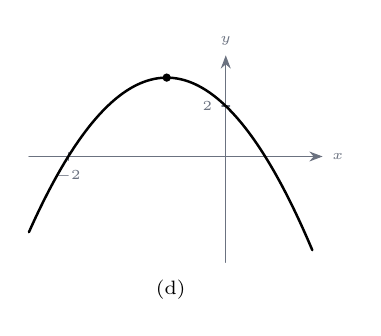
\begin{tikzpicture}
\draw[-Stealth,gray](0.000,1.345)--(3.730,1.345) node[right,font=\tiny]{$x$};
\draw[-Stealth,gray](2.500,0.000)--(2.500,2.630) node[above,font=\tiny]{$y$};
\draw[gray](0.500,1.295)--(0.500,1.395);
\node[below=0pt,gray,font=\tiny] at (0.500,1.295) {$-2$};
\draw[gray](2.450,1.986)--(2.550,1.986);
\node[left=0pt,gray,font=\tiny] at (2.450,1.986) {$2$};
\draw[thick,domain=-2.5:1.1,samples=120,variable=\t] plot({((\t)-(-2.5))/(3.6)*3.6},{((-2*\t*\t - 3*\t + 2)-(-4.199))/(7.803)*2.5});
\fill (1.750,2.347) circle[radius=1.5pt];
\node[font=\scriptsize] at (1.800,-0.340) {(d)};
\end{tikzpicture}
\caption{The four quadratics of question 3. Above the axis $f(x)>0$; on or below it $f(x)\leq 0$. In (c) the curve never reaches the axis, which is why one answer set is everything and the other empty.}
\end{figure}

\begin{figure}[H]
\centering
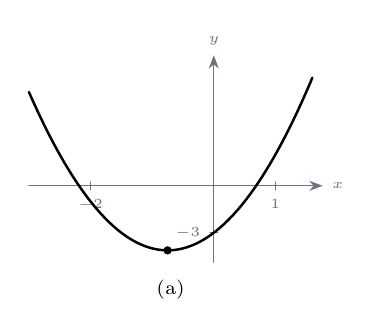
\begin{tikzpicture}
\draw[-Stealth,gray](0.000,0.973)--(3.730,0.973) node[right,font=\tiny]{$x$};
\draw[-Stealth,gray](2.348,0.000)--(2.348,2.630) node[above,font=\tiny]{$y$};
\draw[gray](0.783,0.923)--(0.783,1.023);
\node[below=0pt,gray,font=\tiny] at (0.783,0.923) {$-2$};
\draw[gray](3.130,0.923)--(3.130,1.023);
\node[below=0pt,gray,font=\tiny] at (3.130,0.923) {$1$};
\draw[gray](2.298,0.377)--(2.398,0.377);
\node[left=0pt,gray,font=\tiny] at (2.298,0.377) {$-3$};
\draw[thick,domain=-3.0:1.6,samples=120,variable=\t] plot({((\t)-(-3.0))/(4.6)*3.6},{((2*\t*\t + 3*\t - 3)-(-4.898))/(12.591)*2.5});
\fill (1.761,0.153) circle[radius=1.5pt];
\node[font=\scriptsize] at (1.800,-0.340) {(a)};
\end{tikzpicture}
\hspace{0.35em}
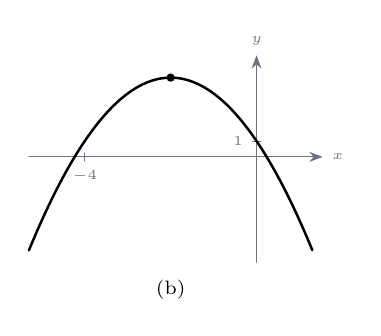
\begin{tikzpicture}
\draw[-Stealth,gray](0.000,1.340)--(3.730,1.340) node[right,font=\tiny]{$x$};
\draw[-Stealth,gray](2.891,0.000)--(2.891,2.630) node[above,font=\tiny]{$y$};
\draw[gray](0.709,1.290)--(0.709,1.390);
\node[below=0pt,gray,font=\tiny] at (0.709,1.290) {$-4$};
\draw[gray](2.841,1.541)--(2.941,1.541);
\node[left=0pt,gray,font=\tiny] at (2.841,1.541) {$1$};
\draw[thick,domain=-5.3:1.3,samples=120,variable=\t] plot({((\t)-(-5.3))/(6.6)*3.6},{((-\t*\t - 4*\t + 1)-(-6.652))/(12.414)*2.5});
\fill (1.800,2.347) circle[radius=1.5pt];
\node[font=\scriptsize] at (1.800,-0.340) {(b)};
\end{tikzpicture}

\vspace{1.4em}

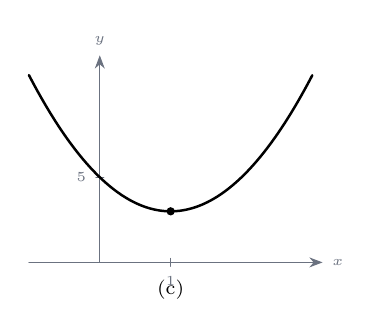
\begin{tikzpicture}
\draw[-Stealth,gray](0.000,0.000)--(3.730,0.000) node[right,font=\tiny]{$x$};
\draw[-Stealth,gray](0.900,0.000)--(0.900,2.630) node[above,font=\tiny]{$y$};
\draw[gray](1.800,-0.050)--(1.800,0.050);
\node[below=0pt,gray,font=\tiny] at (1.800,-0.050) {$1$};
\draw[gray](0.850,1.081)--(0.950,1.081);
\node[left=0pt,gray,font=\tiny] at (0.850,1.081) {$5$};
\draw[thick,domain=-1.0:3.0,samples=120,variable=\t] plot({((\t)-(-1.0))/(4.0)*3.6},{((2*\t*\t - 4*\t + 5)-(0))/(11.56)*2.5});
\fill (1.800,0.649) circle[radius=1.5pt];
\node[font=\scriptsize] at (1.800,-0.340) {(c)};
\end{tikzpicture}
\hspace{0.35em}
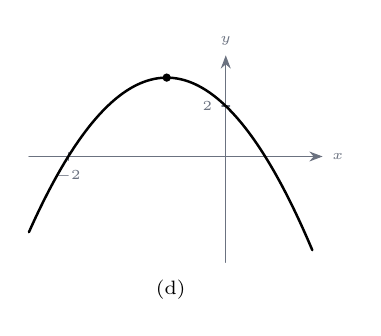
\begin{tikzpicture}
\draw[-Stealth,gray](0.000,1.345)--(3.730,1.345) node[right,font=\tiny]{$x$};
\draw[-Stealth,gray](2.500,0.000)--(2.500,2.630) node[above,font=\tiny]{$y$};
\draw[gray](0.500,1.295)--(0.500,1.395);
\node[below=0pt,gray,font=\tiny] at (0.500,1.295) {$-2$};
\draw[gray](2.450,1.986)--(2.550,1.986);
\node[left=0pt,gray,font=\tiny] at (2.450,1.986) {$2$};
\draw[thick,domain=-2.5:1.1,samples=120,variable=\t] plot({((\t)-(-2.5))/(3.6)*3.6},{((-2*\t*\t - 3*\t + 2)-(-4.199))/(7.803)*2.5});
\fill (1.750,2.347) circle[radius=1.5pt];
\node[font=\scriptsize] at (1.800,-0.340) {(d)};
\end{tikzpicture}
\caption{The four quadratics of question 3. Above the axis $f(x)>0$; on or below it $f(x)\leq 0$. In (c) the curve never reaches the axis, which is why one answer set is everything and the other empty.}
\end{figure}

\begin{note}
Part (c) is the one worth pausing on. A negative discriminant does not mean the question
has no answer --- it means the parabola never crosses the axis, so one of the two sets
is everything and the other is empty. Checking the sign of $f$ at a single convenient
point, here $f(0)=5>0$, settles which is which.
\end{note}
\end{solution}

\begin{problem}
Solve each cubic inequality, illustrating the solution set on a number line.
\quad (a) $4x^3-x<6-9x^2$, \quad (b) $(x+4)(x-2)(x-7)>0$, \quad
(c) $x^3-x^2-9x+9\leq 0$, \quad (d) $4x^3-8x^2-x+2\neq 0$.
\end{problem}

\begin{solution}
The method is the same as for quadratics: get zero on one side, factorise, and use a
sign table across the intervals cut out by the roots.

\textbf{(a).} Rearranging:
$$4x^3+9x^2-x-6<0.$$
Testing candidates dividing $6$: $f(-1)=-4+9+1-6=0$, so $x+1$ is a factor. Dividing,
$$4x^3+9x^2-x-6=(x+1)\left(4x^2+5x-6\right)=(x+1)(4x-3)(x+2),$$
with roots $-2$, $-1$ and $\frac{3}{4}$.

\begin{table}[H]
\centering
\begin{tabular}{|l|c|c|c|c|}
\hline
 & $x<-2$ & $-2<x<-1$ & $-1<x<\frac{3}{4}$ & $x>\frac{3}{4}$\\
\hline
$x+2$ & $-$ & $+$ & $+$ & $+$\\
$x+1$ & $-$ & $-$ & $+$ & $+$\\
$4x-3$ & $-$ & $-$ & $-$ & $+$\\
product & $-$ & $+$ & $-$ & $+$\\
\hline
\end{tabular}
\end{table}

$$\therefore\quad x<-2\quad\text{or}\quad -1<x<\tfrac{3}{4}.$$

\textbf{(b).} Already factorised, roots $-4$, $2$, $7$. With three simple roots the sign
alternates, and the leading coefficient is positive so the rightmost interval is
positive:
$$-,\ +,\ -,\ +\quad\text{across}\quad x<-4,\ -4<x<2,\ 2<x<7,\ x>7.$$
$$\therefore\quad -4<x<2\quad\text{or}\quad x>7.$$

\textbf{(c).} Group:
$$x^3-x^2-9x+9=x^2(x-1)-9(x-1)=\left(x^2-9\right)(x-1)=(x-3)(x+3)(x-1),$$
with roots $-3$, $1$, $3$. Signs alternate, positive on the right:
$$-,\ +,\ -,\ +\quad\text{across}\quad x<-3,\ -3<x<1,\ 1<x<3,\ x>3.$$
$$\therefore\quad x\leq -3\quad\text{or}\quad 1\leq x\leq 3,$$
with the endpoints included since the inequality is $\leq$.

\textbf{(d).} As in Sheet 3, this asks only where the expression is non-zero. Grouping,
$$4x^3-8x^2-x+2=4x^2(x-2)-(x-2)=\left(4x^2-1\right)(x-2)=(2x-1)(2x+1)(x-2),$$
with zeros at $-\frac{1}{2}$, $\frac{1}{2}$ and $2$:
$$\therefore\quad x\in\mathbb{R}-\left\{-\tfrac{1}{2},\ \tfrac{1}{2},\ 2\right\}.$$

\begin{note}
Once a cubic is factorised into three distinct linear factors, the sign simply
alternates between consecutive roots --- there is no need to build the whole table.
Start from the far right, where the sign is that of the leading coefficient, and flip
at each root moving left. A \emph{repeated} factor is the exception: the sign does not
change there.
\end{note}
\end{solution}

\begin{problem}
Sketch each function, and state the values of $x$ for which $f(x)>0$ and $f(x)\leq 0$.
\quad (a) $f(x)=4x^3+9x^2-x-6$, \quad (b) $f(x)=x^3-5x^2-22x+56$, \quad
(c) $f(x)=x^3-5x^2+3x+9$, \quad (d) $f(x)=x^4+4x^3-12x^2$.
\end{problem}

\begin{solution}
\textbf{(a).} Factorised in the previous question as $(x+2)(x+1)(4x-3)$; roots $-2$,
$-1$, $\frac{3}{4}$; $y$-intercept $-6$:
$$f(x)>0:\quad -2<x<-1\ \text{ or }\ x>\tfrac{3}{4},$$
$$f(x)\leq 0:\quad x\leq -2\ \text{ or }\ -1\leq x\leq\tfrac{3}{4}.$$

\textbf{(b).} Testing candidates: $f(2)=8-20-44+56=0$, so $x-2$ is a factor. Dividing,
$$x^3-5x^2-22x+56=(x-2)\left(x^2-3x-28\right)=(x-2)(x-7)(x+4),$$
roots $-4$, $2$, $7$; $y$-intercept $56$:
$$f(x)>0:\quad -4<x<2\ \text{ or }\ x>7,$$
$$f(x)\leq 0:\quad x\leq -4\ \text{ or }\ 2\leq x\leq 7.$$

\textbf{(c).} Testing: $f(3)=27-45+9+9=0$, so $x-3$ is a factor. Dividing,
$$x^3-5x^2+3x+9=(x-3)\left(x^2-2x-3\right)=(x-3)(x-3)(x+1)=(x-3)^2(x+1),$$
a \emph{repeated} root at $x=3$ and a simple root at $x=-1$; $y$-intercept $9$.

Because $(x-3)^2$ is never negative, the sign of $f$ is the sign of $x+1$ everywhere
except at $x=3$, where $f=0$:
$$f(x)>0:\quad x>-1 \text{ but } x\neq 3,$$
$$f(x)\leq 0:\quad x\leq -1\ \text{ or }\ x=3.$$

\textbf{(d).} Take out the common factor first:
$$x^4+4x^3-12x^2=x^2\left(x^2+4x-12\right)=x^2(x+6)(x-2),$$
a repeated root at $x=0$ and simple roots at $-6$ and $2$; $y$-intercept $0$.

Again $x^2\geq 0$, so away from $x=0$ the sign is that of $(x+6)(x-2)$, which is
positive outside $[-6,2]$:
$$f(x)>0:\quad x<-6\ \text{ or }\ x>2,$$
$$f(x)\leq 0:\quad -6\leq x\leq 2.$$

\begin{figure}[H]
\centering
\begin{tikzpicture}[xscale=0.95,yscale=0.16]
\draw[-Stealth,gray](-2,0)--(4.6,0) node[right]{\small $x$};
\draw[-Stealth,gray](0,-6)--(0,22) node[above]{\small $y$};
\foreach \t in {-1,1,2,3,4}{\draw[gray](\t,-0.7)--(\t,0.7); \node[below,gray] at (\t,-1.2){\tiny \t};}
\node[left,gray] at (-0.08,9){\tiny 9};
\draw[thick,domain=-1.35:4.15,samples=100] plot(\x,{(\x-3)^2*(\x+1)});
\fill (-1,0) circle[radius=2.6pt]; \fill (3,0) circle[radius=2.6pt]; \fill (0,9) circle[radius=2.6pt];
\node[above right] at (3,0.4){\tiny touches at $3$};
\end{tikzpicture}
\caption{Part (c), $f(x)=(x-3)^2(x+1)$. The curve crosses at $-1$ but only touches at the repeated root $3$, so the sign does not change there.}
\end{figure}

\begin{figure}[H]
\centering
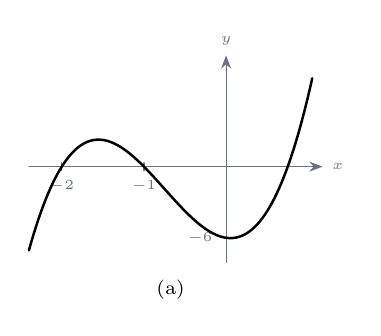
\begin{tikzpicture}
\draw[-Stealth,gray](0.000,1.216)--(3.730,1.216) node[right,font=\tiny]{$x$};
\draw[-Stealth,gray](2.504,0.000)--(2.504,2.630) node[above,font=\tiny]{$y$};
\draw[gray](0.417,1.166)--(0.417,1.266);
\node[below=0pt,gray,font=\tiny] at (0.417,1.166) {$-2$};
\draw[gray](1.461,1.166)--(1.461,1.266);
\node[below=0pt,gray,font=\tiny] at (1.461,1.166) {$-1$};
\draw[gray](2.454,0.313)--(2.554,0.313);
\node[left=0pt,gray,font=\tiny] at (2.454,0.313) {$-6$};
\draw[thick,domain=-2.4:1.05,samples=120,variable=\t] plot({((\t)-(-2.4))/(3.45)*3.6},{((4*\t*\t*\t + 9*\t*\t - \t - 6)-(-8.075))/(16.597)*2.5});
\node[font=\scriptsize] at (1.800,-0.340) {(a)};
\end{tikzpicture}
\hspace{0.35em}
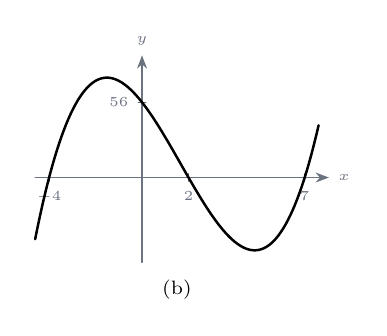
\begin{tikzpicture}
\draw[-Stealth,gray](0.000,1.078)--(3.730,1.078) node[right,font=\tiny]{$x$};
\draw[-Stealth,gray](1.357,0.000)--(1.357,2.630) node[above,font=\tiny]{$y$};
\draw[gray](0.177,1.028)--(0.177,1.128);
\node[below=0pt,gray,font=\tiny] at (0.177,1.028) {$-4$};
\draw[gray](1.948,1.028)--(1.948,1.128);
\node[below=0pt,gray,font=\tiny] at (1.948,1.028) {$2$};
\draw[gray](3.423,1.028)--(3.423,1.128);
\node[below=0pt,gray,font=\tiny] at (3.423,1.028) {$7$};
\draw[gray](1.307,2.033)--(1.407,2.033);
\node[left=0pt,gray,font=\tiny] at (1.307,2.033) {$56$};
\draw[thick,domain=-4.6:7.6,samples=120,variable=\t] plot({((\t)-(-4.6))/(12.2)*3.6},{((\t*\t*\t - 5*\t*\t - 22*\t + 56)-(-63.23))/(146.609)*2.5});
\node[font=\scriptsize] at (1.800,-0.340) {(b)};
\end{tikzpicture}
\hspace{0.35em}
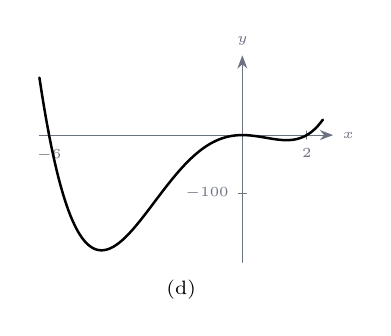
\begin{tikzpicture}
\draw[-Stealth,gray](0.000,1.617)--(3.730,1.617) node[right,font=\tiny]{$x$};
\draw[-Stealth,gray](2.577,0.000)--(2.577,2.630) node[above,font=\tiny]{$y$};
\draw[gray](0.123,1.567)--(0.123,1.667);
\node[below=0pt,gray,font=\tiny] at (0.123,1.567) {$-6$};
\draw[gray](3.395,1.567)--(3.395,1.667);
\node[below=0pt,gray,font=\tiny] at (3.395,1.567) {$2$};
\draw[gray](2.527,0.879)--(2.627,0.879);
\node[left=0pt,gray,font=\tiny] at (2.527,0.879) {$-100$};
\draw[thick,domain=-6.3:2.5,samples=120,variable=\t] plot({((\t)-(-6.3))/(8.8)*3.6},{((\t*\t*\t*\t + 4*\t*\t*\t - 12*\t*\t)-(-219.08))/(338.706)*2.5});
\node[font=\scriptsize] at (1.800,-0.340) {(d)};
\end{tikzpicture}
\caption{The other three functions of question 5. In (d) the repeated root at the origin makes the curve touch the axis there rather than cross.}
\end{figure}

\begin{note}
Parts (c) and (d) both have a repeated root, and that is what makes them different from
(a) and (b). At a repeated root the curve touches the axis and turns back, so the sign
does \emph{not} alternate through it. Answering (c) with ``positive between $-1$ and
$3$, negative after $3$'' is the error the repeated factor is there to catch.
\end{note}

\begin{note}
The point $x=3$ has to be written out of the answer to $f(x)>0$ and into the answer to
$f(x)\leq 0$, because $f(3)=0$ exactly. Isolated points like this are easy to lose.
\end{note}
\end{solution}

\begin{problem}
\begin{enumerate}
\item[(a).] Sketch \quad (i) $y=|2x+3|$, \quad (ii) $y=\left|x^2-9\right|$, \quad
(iii) $y=\left|x^3+1\right|$, \quad (iv) $y=\left|x^3+x^2-x-1\right|$.
\item[(b).] Solve \quad (i) $\left|2x-\frac{3}{2}\right|=3$, \quad
(ii) $|5x-2|=|2x|$.
\end{enumerate}
\end{problem}

\begin{solution}
\textbf{(a).} The graph of $y=|f(x)|$ is the graph of $y=f(x)$ with every part below the
$x$-axis reflected upwards. So sketch $f$ first, then flip.

\textbf{(i).} $y=2x+3$ is a line crossing the axis at $x=-\frac{3}{2}$. Reflecting the
part to the left gives a V with its vertex at $\left(-\frac{3}{2},0\right)$ and
$y$-intercept $3$.

\textbf{(ii).} $y=x^2-9$ is a parabola with roots $\pm 3$ and minimum $(0,-9)$. The
whole arc between $-3$ and $3$ is below the axis, so it flips up into a hump peaking at
$(0,9)$.

\textbf{(iii).} $y=x^3+1$ crosses at $x=-1$. Everything to the left of $-1$ is negative
and flips up, giving a curve that comes down to zero at $x=-1$ and rises again.

\textbf{(iv).} $x^3+x^2-x-1=(x-1)(x+1)^2$, from Sheet 3. It is negative for $x<1$
apart from touching zero at $x=-1$, and positive for $x>1$. After reflection the curve
touches zero at $x=-1$ and again at $x=1$, staying non-negative throughout.

\begin{figure}[H]
\centering
\begin{tikzpicture}[xscale=0.62,yscale=0.22]
\draw[-Stealth,gray](-5,0)--(5,0) node[right]{\small $x$};
\draw[-Stealth,gray](0,-2)--(0,15) node[above]{\small $y$};
\foreach \t in {-3,3}{\draw[gray](\t,-0.6)--(\t,0.6); \node[below,gray] at (\t,-0.9){\tiny \t};}
\node[left,gray] at (-0.15,9){\tiny 9};
\draw[dashed,gray,domain=-3:3,samples=60] plot(\x,{\x*\x-9});
\draw[thick,domain=-4.3:-3,samples=40] plot(\x,{\x*\x-9});
\draw[thick,domain=-3:3,samples=60] plot(\x,{9-\x*\x});
\draw[thick,domain=3:4.3,samples=40] plot(\x,{\x*\x-9});
\fill (0,9) circle[radius=2.6pt];
\node[above right] at (0.1,9.6){\tiny $(0,9)$};
\node[below right,gray] at (1.2,-6.5){\tiny original $x^2-9$};
\end{tikzpicture}
\caption{Part (ii): the dashed arc of $y=x^2-9$ below the axis is reflected upwards to give $y=\left|x^2-9\right|$.}
\end{figure}

\begin{figure}[H]
\centering
\begin{tikzpicture}
\draw[-Stealth,gray](0.000,0.149)--(3.730,0.149) node[right,font=\tiny]{$x$};
\draw[-Stealth,gray](2.571,0.000)--(2.571,2.630) node[above,font=\tiny]{$y$};
\draw[gray](0.643,0.099)--(0.643,0.199);
\node[below=0pt,gray,font=\tiny] at (0.643,0.099) {$-3$};
\draw[gray](3.214,0.099)--(3.214,0.199);
\node[below=0pt,gray,font=\tiny] at (3.214,0.099) {$1$};
\draw[gray](2.521,1.212)--(2.621,1.212);
\node[left=0pt,gray,font=\tiny] at (2.521,1.212) {$3$};
\draw[thick,domain=-4.0:1.6,samples=120,variable=\t] plot({((\t)-(-4.0))/(5.6)*3.6},{((abs(2*\t+3))-(-0.421))/(7.054)*2.5});
\fill (1.607,0.149) circle[radius=1.5pt];
\node[font=\scriptsize] at (1.800,-0.340) {(i) $|2x+3|$};
\end{tikzpicture}
\hspace{0.35em}
\begin{tikzpicture}
\draw[-Stealth,gray](0.000,0.143)--(3.730,0.143) node[right,font=\tiny]{$x$};
\draw[-Stealth,gray](1.800,0.000)--(1.800,2.630) node[above,font=\tiny]{$y$};
\draw[gray](0.573,0.093)--(0.573,0.193);
\node[below=0pt,gray,font=\tiny] at (0.573,0.093) {$-3$};
\draw[gray](3.027,0.093)--(3.027,0.193);
\node[below=0pt,gray,font=\tiny] at (3.027,0.093) {$3$};
\draw[gray](1.750,2.057)--(1.850,2.057);
\node[left=0pt,gray,font=\tiny] at (1.750,2.057) {$9$};
\draw[thick,domain=-4.4:4.4,samples=120,variable=\t] plot({((\t)-(-4.4))/(8.8)*3.6},{((abs(\t*\t-9))-(-0.674))/(11.756)*2.5});
\fill (1.800,2.057) circle[radius=1.5pt];
\node[font=\scriptsize] at (1.800,-0.340) {(ii) $\left|x^2-9\right|$};
\end{tikzpicture}

\vspace{1.4em}

\begin{tikzpicture}
\draw[-Stealth,gray](0.000,0.152)--(3.730,0.152) node[right,font=\tiny]{$x$};
\draw[-Stealth,gray](2.084,0.000)--(2.084,2.630) node[above,font=\tiny]{$y$};
\draw[gray](1.137,0.102)--(1.137,0.202);
\node[below=0pt,gray,font=\tiny] at (1.137,0.102) {$-1$};
\draw[gray](3.032,0.102)--(3.032,0.202);
\node[below=0pt,gray,font=\tiny] at (3.032,0.102) {$1$};
\draw[gray](2.034,0.379)--(2.134,0.379);
\node[left=0pt,gray,font=\tiny] at (2.034,0.379) {$1$};
\draw[thick,domain=-2.2:1.6,samples=120,variable=\t] plot({((\t)-(-2.2))/(3.8000000000000003)*3.6},{((abs(\t*\t*\t+1))-(-0.666))/(10.989)*2.5});
\fill (1.137,0.152) circle[radius=1.5pt];
\node[font=\scriptsize] at (1.800,-0.340) {(iii) $\left|x^3+1\right|$};
\end{tikzpicture}
\hspace{0.35em}
\begin{tikzpicture}
\draw[-Stealth,gray](0.000,0.153)--(3.730,0.153) node[right,font=\tiny]{$x$};
\draw[-Stealth,gray](2.070,0.000)--(2.070,2.630) node[above,font=\tiny]{$y$};
\draw[gray](1.170,0.103)--(1.170,0.203);
\node[below=0pt,gray,font=\tiny] at (1.170,0.103) {$-1$};
\draw[gray](2.970,0.103)--(2.970,0.203);
\node[below=0pt,gray,font=\tiny] at (2.970,0.103) {$1$};
\draw[gray](2.020,0.547)--(2.120,0.547);
\node[left=0pt,gray,font=\tiny] at (2.020,0.547) {$1$};
\draw[thick,domain=-2.3:1.7,samples=120,variable=\t] plot({((\t)-(-2.3))/(4.0)*3.6},{((abs(\t*\t*\t+\t*\t-\t-1))-(-0.39))/(6.356999999999999)*2.5});
\fill (1.170,0.153) circle[radius=1.5pt];
\fill (2.970,0.153) circle[radius=1.5pt];
\node[font=\scriptsize] at (1.800,-0.340) {(iv) $\left|x^3+x^2-x-1\right|$};
\end{tikzpicture}
\caption{All four graphs of question 6(a). Each is the ordinary curve with everything below the axis folded upwards, so none goes below $y=0$; in (iv) the curve touches the axis at $x=-1$ as well as at $x=1$.}
\end{figure}

\begin{figure}[H]
\centering
\begin{tikzpicture}
\draw[-Stealth,gray](0.000,0.149)--(3.730,0.149) node[right,font=\tiny]{$x$};
\draw[-Stealth,gray](2.571,0.000)--(2.571,2.630) node[above,font=\tiny]{$y$};
\draw[gray](0.643,0.099)--(0.643,0.199);
\node[below=0pt,gray,font=\tiny] at (0.643,0.099) {$-3$};
\draw[gray](3.214,0.099)--(3.214,0.199);
\node[below=0pt,gray,font=\tiny] at (3.214,0.099) {$1$};
\draw[gray](2.521,1.212)--(2.621,1.212);
\node[left=0pt,gray,font=\tiny] at (2.521,1.212) {$3$};
\draw[thick,domain=-4.0:1.6,samples=120,variable=\t] plot({((\t)-(-4.0))/(5.6)*3.6},{((abs(2*\t+3))-(-0.421))/(7.054)*2.5});
\fill (1.607,0.149) circle[radius=1.5pt];
\node[font=\scriptsize] at (1.800,-0.340) {(i) $|2x+3|$};
\end{tikzpicture}
\hspace{0.35em}
\begin{tikzpicture}
\draw[-Stealth,gray](0.000,0.143)--(3.730,0.143) node[right,font=\tiny]{$x$};
\draw[-Stealth,gray](1.800,0.000)--(1.800,2.630) node[above,font=\tiny]{$y$};
\draw[gray](0.573,0.093)--(0.573,0.193);
\node[below=0pt,gray,font=\tiny] at (0.573,0.093) {$-3$};
\draw[gray](3.027,0.093)--(3.027,0.193);
\node[below=0pt,gray,font=\tiny] at (3.027,0.093) {$3$};
\draw[gray](1.750,2.057)--(1.850,2.057);
\node[left=0pt,gray,font=\tiny] at (1.750,2.057) {$9$};
\draw[thick,domain=-4.4:4.4,samples=120,variable=\t] plot({((\t)-(-4.4))/(8.8)*3.6},{((abs(\t*\t-9))-(-0.674))/(11.756)*2.5});
\fill (1.800,2.057) circle[radius=1.5pt];
\node[font=\scriptsize] at (1.800,-0.340) {(ii) $\left|x^2-9\right|$};
\end{tikzpicture}

\vspace{1.4em}

\begin{tikzpicture}
\draw[-Stealth,gray](0.000,0.152)--(3.730,0.152) node[right,font=\tiny]{$x$};
\draw[-Stealth,gray](2.084,0.000)--(2.084,2.630) node[above,font=\tiny]{$y$};
\draw[gray](1.137,0.102)--(1.137,0.202);
\node[below=0pt,gray,font=\tiny] at (1.137,0.102) {$-1$};
\draw[gray](3.032,0.102)--(3.032,0.202);
\node[below=0pt,gray,font=\tiny] at (3.032,0.102) {$1$};
\draw[gray](2.034,0.379)--(2.134,0.379);
\node[left=0pt,gray,font=\tiny] at (2.034,0.379) {$1$};
\draw[thick,domain=-2.2:1.6,samples=120,variable=\t] plot({((\t)-(-2.2))/(3.8000000000000003)*3.6},{((abs(\t*\t*\t+1))-(-0.666))/(10.989)*2.5});
\fill (1.137,0.152) circle[radius=1.5pt];
\node[font=\scriptsize] at (1.800,-0.340) {(iii) $\left|x^3+1\right|$};
\end{tikzpicture}
\hspace{0.35em}
\begin{tikzpicture}
\draw[-Stealth,gray](0.000,0.153)--(3.730,0.153) node[right,font=\tiny]{$x$};
\draw[-Stealth,gray](2.070,0.000)--(2.070,2.630) node[above,font=\tiny]{$y$};
\draw[gray](1.170,0.103)--(1.170,0.203);
\node[below=0pt,gray,font=\tiny] at (1.170,0.103) {$-1$};
\draw[gray](2.970,0.103)--(2.970,0.203);
\node[below=0pt,gray,font=\tiny] at (2.970,0.103) {$1$};
\draw[gray](2.020,0.547)--(2.120,0.547);
\node[left=0pt,gray,font=\tiny] at (2.020,0.547) {$1$};
\draw[thick,domain=-2.3:1.7,samples=120,variable=\t] plot({((\t)-(-2.3))/(4.0)*3.6},{((abs(\t*\t*\t+\t*\t-\t-1))-(-0.39))/(6.356999999999999)*2.5});
\fill (1.170,0.153) circle[radius=1.5pt];
\fill (2.970,0.153) circle[radius=1.5pt];
\node[font=\scriptsize] at (1.800,-0.340) {(iv) $\left|x^3+x^2-x-1\right|$};
\end{tikzpicture}
\caption{All four graphs of question 6(a). Each is the ordinary curve with everything below the axis folded upwards, so none goes below $y=0$; in (iv) the curve touches the axis at $x=-1$ as well as at $x=1$.}
\end{figure}

\textbf{(b)(i).} $|A|=3$ means $A=3$ or $A=-3$:
$$2x-\tfrac{3}{2}=3\quad\implies\quad 2x=\tfrac{9}{2}\quad\implies\quad x=\tfrac{9}{4},$$
$$2x-\tfrac{3}{2}=-3\quad\implies\quad 2x=-\tfrac{3}{2}\quad\implies\quad
x=-\tfrac{3}{4}.$$
$$\therefore\quad x=\tfrac{9}{4}\ \text{ or }\ x=-\tfrac{3}{4}.$$

\textbf{(ii).} $|A|=|B|$ means $A=B$ or $A=-B$:
$$5x-2=2x\quad\implies\quad 3x=2\quad\implies\quad x=\tfrac{2}{3},$$
$$5x-2=-2x\quad\implies\quad 7x=2\quad\implies\quad x=\tfrac{2}{7}.$$
$$\therefore\quad x=\tfrac{2}{3}\ \text{ or }\ x=\tfrac{2}{7}.$$

\textbf{Check.} At $x=\frac{2}{3}$: $\left|\frac{10}{3}-2\right|=\frac{4}{3}$ and
$\left|\frac{4}{3}\right|=\frac{4}{3}$. $\checkmark$ \ At $x=\frac{2}{7}$:
$\left|\frac{10}{7}-2\right|=\frac{4}{7}$ and $\left|\frac{4}{7}\right|=\frac{4}{7}$.
$\checkmark$

\begin{note}
When both sides carry a modulus, as in (ii), no check on signs is needed --- both cases
always give genuine solutions. When only one side does, as in the next question, the
other side must be non-negative, and any root failing that has to be discarded.
\end{note}
\end{solution}

\begin{problem}
For each pair, sketch the graphs and solve $f(x)=g(x)$.
\begin{enumerate}
\item[(i).] $f(x)=\left|x^2-2x\right|$, \quad $g(x)=\frac{1}{4}-2x$
\item[(ii).] $f(x)=-2x$, \quad $g(x)=\left|\frac{1}{2}x-2\right|$
\item[(iii).] $f(x)=|5x-4|$, \quad $g(x)=24+2x-x^2$
\end{enumerate}
\end{problem}

\begin{solution}
Each has a modulus on one side only. Split into the two cases, solve each, and then
\emph{test every root} against the case it came from and against the requirement that
the non-modulus side be non-negative.

\textbf{(i).} $\left|x^2-2x\right|=\frac{1}{4}-2x$. Note $x^2-2x=x(x-2)$, which is
$\geq 0$ for $x\leq 0$ or $x\geq 2$, and negative for $0<x<2$.

\emph{Case 1: $x\leq 0$ or $x\geq 2$.} The modulus comes off unchanged:
$$x^2-2x=\tfrac{1}{4}-2x\quad\implies\quad x^2=\tfrac{1}{4}\quad\implies\quad
x=\pm\tfrac{1}{2}.$$
Of these, $x=-\frac{1}{2}$ lies in the case and $x=\frac{1}{2}$ does not. Keep
$x=-\frac{1}{2}$.

\emph{Case 2: $0<x<2$.} The modulus comes off with a sign change:
$$-\left(x^2-2x\right)=\tfrac{1}{4}-2x\quad\implies\quad -x^2+4x-\tfrac{1}{4}=0
\quad\implies\quad x^2-4x+\tfrac{1}{4}=0,$$
$$x=\frac{4\pm\sqrt{16-1}}{2}=\frac{4\pm\sqrt{15}}{2}=2\pm\frac{\sqrt{15}}{2}
\approx 3.94 \text{ and } 0.064.$$
Only $x=2-\frac{\sqrt{15}}{2}\approx 0.064$ lies in $(0,2)$.

Finally check the right-hand side is non-negative at both surviving roots:
$\frac{1}{4}-2\left(-\frac{1}{2}\right)=\frac{5}{4}>0$ and
$\frac{1}{4}-2(0.064)\approx 0.12>0$. Both stand.
$$\therefore\quad x=-\tfrac{1}{2}\quad\text{or}\quad x=2-\tfrac{\sqrt{15}}{2}
\approx 0.064.$$

\textbf{(ii).} $-2x=\left|\frac{1}{2}x-2\right|$. A modulus is never negative, so
$-2x\geq 0$, giving $x\leq 0$ before anything else is done.

\emph{Case 1: $\frac{1}{2}x-2\geq 0$, that is $x\geq 4$.} This contradicts $x\leq 0$, so
this case is empty. (Solving it anyway gives $x=\frac{4}{5}$, which fails both
conditions.)

\emph{Case 2: $x<4$.}
$$-2x=-\left(\tfrac{1}{2}x-2\right)=2-\tfrac{1}{2}x\quad\implies\quad
-2x+\tfrac{1}{2}x=2\quad\implies\quad -\tfrac{3}{2}x=2\quad\implies\quad
x=-\tfrac{4}{3}.$$
This satisfies $x<4$ and $x\leq 0$.
$$\therefore\quad x=-\tfrac{4}{3}.$$

\textbf{Check.} $-2\left(-\frac{4}{3}\right)=\frac{8}{3}$, and
$\left|\frac{1}{2}\left(-\frac{4}{3}\right)-2\right|=\left|-\frac{2}{3}-2\right|
=\frac{8}{3}$. $\checkmark$

\textbf{(iii).} $|5x-4|=24+2x-x^2$. The modulus is zero at $x=\frac{4}{5}$.

\emph{Case 1: $x\geq\frac{4}{5}$.}
$$5x-4=24+2x-x^2\quad\implies\quad x^2+3x-28=0\quad\implies\quad (x+7)(x-4)=0,$$
giving $x=-7$ or $x=4$. Only $x=4$ lies in the case.

\emph{Case 2: $x<\frac{4}{5}$.}
$$-(5x-4)=24+2x-x^2\quad\implies\quad 4-5x=24+2x-x^2\quad\implies\quad
x^2-7x-20=0,$$
$$x=\frac{7\pm\sqrt{49+80}}{2}=\frac{7\pm\sqrt{129}}{2}\approx 9.18 \text{ and } -2.18.$$
Only $x=\frac{7-\sqrt{129}}{2}\approx -2.18$ lies in the case.

Both surviving roots need $24+2x-x^2\geq 0$: at $x=4$ it is $24+8-16=16>0$, and at
$x\approx -2.18$ it is $\approx 14.9>0$.
$$\therefore\quad x=4\quad\text{or}\quad x=\frac{7-\sqrt{129}}{2}\approx -2.18.$$

\begin{figure}[H]
\centering
\begin{tikzpicture}
\draw[-Stealth,gray](0.000,1.121)--(3.730,1.121) node[right,font=\tiny]{$x$};
\draw[-Stealth,gray](1.543,0.000)--(1.543,2.630) node[above,font=\tiny]{$y$};
\draw[gray](0.257,1.071)--(0.257,1.171);
\node[below=0pt,gray,font=\tiny] at (0.257,1.071) {$-1$};
\draw[gray](2.829,1.071)--(2.829,1.171);
\node[below=0pt,gray,font=\tiny] at (2.829,1.071) {$1$};
\draw[thick,domain=-1.2:1.6,samples=120,variable=\t] plot({((\t)-(-1.2))/(2.8)*3.6},{((abs(\t*\t-2*\t))-(-3.342))/(7.449999999999999)*2.5});
\draw[thick,dashed,domain=-1.2:1.6,samples=120,variable=\t] plot({((\t)-(-1.2))/(2.8)*3.6},{((0.25-2*\t)-(-3.342))/(7.449999999999999)*2.5});
\fill (0.900,1.541) circle[radius=1.5pt];
\fill (1.625,1.163) circle[radius=1.5pt];
\node[font=\scriptsize] at (1.800,-0.340) {(i) $\left|x^2-2x\right|$ and $\frac14-2x$};
\end{tikzpicture}
\hspace{0.35em}
\begin{tikzpicture}
\draw[-Stealth,gray](0.000,1.334)--(3.730,1.334) node[right,font=\tiny]{$x$};
\draw[-Stealth,gray](1.662,0.000)--(1.662,2.630) node[above,font=\tiny]{$y$};
\draw[gray](0.554,1.284)--(0.554,1.384);
\node[below=0pt,gray,font=\tiny] at (0.554,1.284) {$-2$};
\draw[gray](2.769,1.284)--(2.769,1.384);
\node[below=0pt,gray,font=\tiny] at (2.769,1.284) {$2$};
\draw[thick,domain=-3.0:3.5,samples=120,variable=\t] plot({((\t)-(-3.0))/(6.5)*3.6},{((-2*\t)-(-7.91))/(14.82)*2.5});
\draw[thick,dashed,domain=-3.0:3.5,samples=120,variable=\t] plot({((\t)-(-3.0))/(6.5)*3.6},{((abs(\t/2-2))-(-7.91))/(14.82)*2.5});
\fill (0.923,1.784) circle[radius=1.5pt];
\node[font=\scriptsize] at (1.800,-0.340) {(ii) $-2x$ and $\left|\frac12x-2\right|$};
\end{tikzpicture}

\vspace{1.4em}

\begin{tikzpicture}
\draw[-Stealth,gray](0.000,0.486)--(3.730,0.486) node[right,font=\tiny]{$x$};
\draw[-Stealth,gray](1.473,0.000)--(1.473,2.630) node[above,font=\tiny]{$y$};
\draw[gray](0.164,0.436)--(0.164,0.536);
\node[below=0pt,gray,font=\tiny] at (0.164,0.436) {$-4$};
\draw[gray](2.782,0.436)--(2.782,0.536);
\node[below=0pt,gray,font=\tiny] at (2.782,0.436) {$4$};
\draw[gray](3.436,0.436)--(3.436,0.536);
\node[below=0pt,gray,font=\tiny] at (3.436,0.436) {$6$};
\draw[thick,domain=-4.5:6.5,samples=120,variable=\t] plot({((\t)-(-4.5))/(11.0)*3.6},{((abs(5*\t-4))-(-7.367))/(37.859)*2.5});
\draw[thick,dashed,domain=-4.5:6.5,samples=120,variable=\t] plot({((\t)-(-4.5))/(11.0)*3.6},{((24+2*\t-\t*\t)-(-7.367))/(37.859)*2.5});
\fill (2.782,1.543) circle[radius=1.5pt];
\fill (0.760,1.470) circle[radius=1.5pt];
\node[font=\scriptsize] at (1.800,-0.340) {(iii) $|5x-4|$ and $24+2x-x^2$};
\end{tikzpicture}
\caption{Question 6(c): the modulus graph solid, the other curve dashed. The marked points are the solutions --- two in (i), one in (ii), two in (iii) --- and counting the crossings checks that no root was wrongly kept or discarded.}
\end{figure}

\begin{figure}[H]
\centering
\begin{tikzpicture}
\draw[-Stealth,gray](0.000,1.121)--(3.730,1.121) node[right,font=\tiny]{$x$};
\draw[-Stealth,gray](1.543,0.000)--(1.543,2.630) node[above,font=\tiny]{$y$};
\draw[gray](0.257,1.071)--(0.257,1.171);
\node[below=0pt,gray,font=\tiny] at (0.257,1.071) {$-1$};
\draw[gray](2.829,1.071)--(2.829,1.171);
\node[below=0pt,gray,font=\tiny] at (2.829,1.071) {$1$};
\draw[thick,domain=-1.2:1.6,samples=120,variable=\t] plot({((\t)-(-1.2))/(2.8)*3.6},{((abs(\t*\t-2*\t))-(-3.342))/(7.449999999999999)*2.5});
\draw[thick,dashed,domain=-1.2:1.6,samples=120,variable=\t] plot({((\t)-(-1.2))/(2.8)*3.6},{((0.25-2*\t)-(-3.342))/(7.449999999999999)*2.5});
\fill (0.900,1.541) circle[radius=1.5pt];
\fill (1.625,1.163) circle[radius=1.5pt];
\node[font=\scriptsize] at (1.800,-0.340) {(i) $\left|x^2-2x\right|$ and $\frac14-2x$};
\end{tikzpicture}
\hspace{0.35em}
\begin{tikzpicture}
\draw[-Stealth,gray](0.000,1.334)--(3.730,1.334) node[right,font=\tiny]{$x$};
\draw[-Stealth,gray](1.662,0.000)--(1.662,2.630) node[above,font=\tiny]{$y$};
\draw[gray](0.554,1.284)--(0.554,1.384);
\node[below=0pt,gray,font=\tiny] at (0.554,1.284) {$-2$};
\draw[gray](2.769,1.284)--(2.769,1.384);
\node[below=0pt,gray,font=\tiny] at (2.769,1.284) {$2$};
\draw[thick,domain=-3.0:3.5,samples=120,variable=\t] plot({((\t)-(-3.0))/(6.5)*3.6},{((-2*\t)-(-7.91))/(14.82)*2.5});
\draw[thick,dashed,domain=-3.0:3.5,samples=120,variable=\t] plot({((\t)-(-3.0))/(6.5)*3.6},{((abs(\t/2-2))-(-7.91))/(14.82)*2.5});
\fill (0.923,1.784) circle[radius=1.5pt];
\node[font=\scriptsize] at (1.800,-0.340) {(ii) $-2x$ and $\left|\frac12x-2\right|$};
\end{tikzpicture}

\vspace{1.4em}

\begin{tikzpicture}
\draw[-Stealth,gray](0.000,0.486)--(3.730,0.486) node[right,font=\tiny]{$x$};
\draw[-Stealth,gray](1.473,0.000)--(1.473,2.630) node[above,font=\tiny]{$y$};
\draw[gray](0.164,0.436)--(0.164,0.536);
\node[below=0pt,gray,font=\tiny] at (0.164,0.436) {$-4$};
\draw[gray](2.782,0.436)--(2.782,0.536);
\node[below=0pt,gray,font=\tiny] at (2.782,0.436) {$4$};
\draw[gray](3.436,0.436)--(3.436,0.536);
\node[below=0pt,gray,font=\tiny] at (3.436,0.436) {$6$};
\draw[thick,domain=-4.5:6.5,samples=120,variable=\t] plot({((\t)-(-4.5))/(11.0)*3.6},{((abs(5*\t-4))-(-7.367))/(37.859)*2.5});
\draw[thick,dashed,domain=-4.5:6.5,samples=120,variable=\t] plot({((\t)-(-4.5))/(11.0)*3.6},{((24+2*\t-\t*\t)-(-7.367))/(37.859)*2.5});
\fill (2.782,1.543) circle[radius=1.5pt];
\fill (0.760,1.470) circle[radius=1.5pt];
\node[font=\scriptsize] at (1.800,-0.340) {(iii) $|5x-4|$ and $24+2x-x^2$};
\end{tikzpicture}
\caption{Question 6(c): the modulus graph solid, the other curve dashed. The marked points are the solutions --- two in (i), one in (ii), two in (iii) --- and counting the crossings checks that no root was wrongly kept or discarded.}
\end{figure}

\begin{note}
Every part here produced a candidate that had to be thrown away: $\frac{1}{2}$ in (i),
$\frac{4}{5}$ in (ii), and $-7$ and $9.18$ in (iii). Splitting into cases generates
roots that solve the equation \emph{without} the modulus but not with it, so testing
each root against its own case is not optional --- it is where half the marks are.
\end{note}

\begin{note}
The sketch is worth doing first even when the algebra is straightforward, because it
tells you how many intersections to expect. If the algebra produces three surviving
roots and the picture shows two crossings, something has gone wrong.
\end{note}
\end{solution}


\begin{note}
\textbf{Tutorial Sheet 5} (an earlier version of this material, dated April 2023)
repeats much of Sheets 3 and 4 word for word. Its question 3 is Sheet 3's question 6(c),
its question 4(a)--(e) is Sheet 3's question 7, its question 6 is Sheet 3's question 8,
its question 7(b)--(e) is Sheet 3's question 9(c)--(f), and its question 8 is Sheet 4's
question 1(a) --- including the same misprint in $x^4-6x^3-11x^2+24x-28$. All of those
are solved above and are not repeated here.

What follows is the genuinely new material from Sheet 5: its questions 1 and 2, which
use different divisors; question 4(f); question 5; the two new sketches in question 7;
and question 9, on partial fractions, which appears nowhere else.
\end{note}

\begin{problem}
Use long division to divide each polynomial by the given divisor.
\begin{enumerate}
\item[(a).] $f(x)=-x^2+3x+5$ by $x^2+1$
\item[(b).] $f(x)=5x^3-19x^2+16x-4$ by $x-5$
\item[(c).] $f(x)=2x^3+6x^2-x+3$ by $2x^2-2$
\item[(d).] $f(x)=-2x^4+3x^2+1$ by $x^2-2x+3$
\end{enumerate}
\end{problem}

\begin{solution}
\textbf{(a).} The dividend and divisor have the \emph{same} degree, so the quotient is a
constant:
$$-x^2\div x^2=-1;\quad -1\left(x^2+1\right)=-x^2-1;\quad
\text{subtract: } 3x+5-(-1)=3x+6.$$
The remainder $3x+6$ has degree $1$, lower than the divisor's $2$, so we stop.
$$\therefore\quad -x^2+3x+5=(-1)\left(x^2+1\right)+(3x+6).$$

\textbf{(b).} Note the divisor here is $x-5$, not the $x-2$ of Sheet 3:
$$5x^3\div x=5x^2;\quad 5x^2(x-5)=5x^3-25x^2;\quad \text{subtract: } 6x^2+16x-4.$$
$$6x^2\div x=6x;\quad 6x(x-5)=6x^2-30x;\quad \text{subtract: } 46x-4.$$
$$46x\div x=46;\quad 46(x-5)=46x-230;\quad \text{subtract: } 226.$$
$$\therefore\quad 5x^3-19x^2+16x-4=\left(5x^2+6x+46\right)(x-5)+226.$$

\textbf{(c).} Writing the divisor as $2x^2+0x-2$:
$$2x^3\div 2x^2=x;\quad x\left(2x^2-2\right)=2x^3-2x;\quad
\text{subtract: } 6x^2+x+3.$$
$$6x^2\div 2x^2=3;\quad 3\left(2x^2-2\right)=6x^2-6;\quad \text{subtract: } x+9.$$
$$\therefore\quad 2x^3+6x^2-x+3=(x+3)\left(2x^2-2\right)+(x+9).$$

\textbf{(d).} Write the dividend in full as $-2x^4+0x^3+3x^2+0x+1$:
$$-2x^4\div x^2=-2x^2;\quad -2x^2\left(x^2-2x+3\right)=-2x^4+4x^3-6x^2;$$
$$\text{subtract: } -4x^3+9x^2+0x+1.$$
$$-4x^3\div x^2=-4x;\quad -4x\left(x^2-2x+3\right)=-4x^3+8x^2-12x;\quad
\text{subtract: } x^2+12x+1.$$
$$x^2\div x^2=1;\quad 1\left(x^2-2x+3\right)=x^2-2x+3;\quad
\text{subtract: } 14x-2.$$
$$\therefore\quad -2x^4+3x^2+1=\left(-2x^2-4x+1\right)\left(x^2-2x+3\right)+(14x-2).$$

\begin{note}
Part (a) is worth noticing: when the dividend and divisor have the same degree the
quotient is a number, and when the dividend has the \emph{lower} degree the quotient is
zero and the whole dividend is the remainder. Neither case is an error.
\end{note}
\end{solution}

\begin{problem}
Use synthetic division to divide each polynomial by the given divisor, writing the
result as $p(x)=q(x)(x-a)+r$.
\begin{enumerate}
\item[(a).] $p(x)=x^3-7x^2-4x+28$ by $x-3$
\item[(b).] $p(x)=5x^3-6x^2-28x-2$ by $5x+10$
\item[(c).] $p(x)=x^3-10x^2-31x-30$ by $x-11$
\item[(d).] $p(x)=6x^3+x^2-21x-10$ by $2x+1$
\end{enumerate}
\end{problem}

\begin{solution}
\textbf{(a).} Divisor $x-3$, so $a=3$:

\begin{table}[H]
\centering
\begin{tabular}{|c|r r r r|}
\hline
$a=3$ & 1 & $-7$ & $-4$ & 28\\
      &   & 3 & $-12$ & $-48$\\
\hline
      & 1 & $-4$ & $-16$ & $\mathbf{-20}$\\
\hline
\end{tabular}
\end{table}

$$\therefore\quad x^3-7x^2-4x+28=\left(x^2-4x-16\right)(x-3)-20.$$
Compare Sheet 3, where the same polynomial divided by $x+2$ gave remainder $0$. Here
$x-3$ is not a factor.

\textbf{(b).} The divisor is $5x+10=5(x+2)$, so first divide by $x+2$, that is $a=-2$:

\begin{table}[H]
\centering
\begin{tabular}{|c|r r r r|}
\hline
$a=-2$ & 5 & $-6$ & $-28$ & $-2$\\
       &   & $-10$ & 32 & $-8$\\
\hline
       & 5 & $-16$ & 4 & $\mathbf{-10}$\\
\hline
\end{tabular}
\end{table}

$$5x^3-6x^2-28x-2=\left(5x^2-16x+4\right)(x+2)-10.$$
Now convert to the required divisor. Since $x+2=\frac{1}{5}(5x+10)$, move the
$\frac{1}{5}$ into the quotient:
$$=\left(x^2-\tfrac{16}{5}x+\tfrac{4}{5}\right)(5x+10)-10.$$

\textbf{(c).} Divisor $x-11$, so $a=11$:

\begin{table}[H]
\centering
\begin{tabular}{|c|r r r r|}
\hline
$a=11$ & 1 & $-10$ & $-31$ & $-30$\\
       &   & 11 & 11 & $-220$\\
\hline
       & 1 & 1 & $-20$ & $\mathbf{-250}$\\
\hline
\end{tabular}
\end{table}

$$\therefore\quad x^3-10x^2-31x-30=\left(x^2+x-20\right)(x-11)-250.$$

\textbf{(d).} This is the same as Sheet 3, question 6(b)(iv):
$$6x^3+x^2-21x-10=\left(3x^2-x-10\right)(2x+1)+0.$$

\begin{note}
Parts (b) and (d) both have a divisor whose leading coefficient is not $1$, and both
need the same adjustment: divide by the corresponding $x-a$, then move the constant
factor from the divisor into the quotient. The remainder is unaffected --- it is
$p(a)$ either way.
\end{note}

\begin{note}
Each remainder here can be checked against the remainder theorem. In (c),
$p(11)=1331-1210-341-30=-250$. $\checkmark$
\end{note}
\end{solution}

\begin{problem}
Solve $x^3-8=0$.
\end{problem}

\begin{solution}
This is a difference of two cubes, $a^3-b^3=(a-b)\left(a^2+ab+b^2\right)$ with $a=x$ and
$b=2$:
$$x^3-8=(x-2)\left(x^2+2x+4\right)=0.$$
The first factor gives $x=2$. For the second,
$$\Delta=4-16=-12<0,$$
so it has no real roots.
$$\therefore\quad x=2 \text{ is the only real solution}.$$

\begin{note}
Every cubic with real coefficients has at least one real root, and here it is the
obvious one. The other two roots are complex, $x=-1\pm i\sqrt{3}$, and if the question
had asked for solutions in $\mathbb{C}$ they would need to be given as well.
\end{note}
\end{solution}

\begin{problem}
Let $f(x)=4x^3-7x-3$.
\begin{enumerate}
\item[(a).] Find the remainder when $f(x)$ is divided by $x-2$.
\item[(b).] Show that $2x+1$ is a factor of $f(x)$.
\item[(c).] Hence, or otherwise, solve $4x^3-7x-3=0$.
\end{enumerate}
\end{problem}

\begin{solution}
\textbf{(a).} By the remainder theorem the remainder is $f(2)$:
$$f(2)=4(8)-7(2)-3=32-14-3=15.$$

\textbf{(b).} The divisor $2x+1$ vanishes at $x=-\frac{1}{2}$, so by the factor theorem
it is a factor precisely when $f\left(-\frac{1}{2}\right)=0$:
$$f\left(-\tfrac{1}{2}\right)=4\left(-\tfrac{1}{8}\right)-7\left(-\tfrac{1}{2}\right)-3
=-\tfrac{1}{2}+\tfrac{7}{2}-3=3-3=0.$$
$$\therefore\quad 2x+1 \text{ is a factor}.$$

\textbf{(c).} Dividing $f(x)$ by $2x+1$. Writing the dividend in full as
$4x^3+0x^2-7x-3$ and using synthetic division with $a=-\frac{1}{2}$:

\begin{table}[H]
\centering
\begin{tabular}{|c|r r r r|}
\hline
$a=-\frac{1}{2}$ & 4 & 0 & $-7$ & $-3$\\
                 &   & $-2$ & 1 & 3\\
\hline
                 & 4 & $-2$ & $-6$ & \textbf{0}\\
\hline
\end{tabular}
\end{table}

$$4x^3-7x-3=\left(4x^2-2x-6\right)\left(x+\tfrac{1}{2}\right)
=\left(2x^2-x-3\right)(2x+1),$$
halving the quotient because $x+\frac{1}{2}=\frac{1}{2}(2x+1)$. Factorising the
quadratic:
$$2x^2-x-3=(2x-3)(x+1).$$
$$\therefore\quad 4x^3-7x-3=(2x+1)(2x-3)(x+1)=0,$$
$$x=-\tfrac{1}{2},\qquad x=\tfrac{3}{2},\qquad x=-1.$$

\begin{note}
Parts (a) and (b) are the same theorem used twice: substitute the value that makes the
divisor zero. The only difference is that in (b) the answer happens to be zero, which is
what ``factor'' means. Part (a) is not needed for part (c) --- it is there to make the
contrast.
\end{note}
\end{solution}

\begin{problem}
Sketch, indicating the $x$- and $y$-intercepts:
\quad (a) $f(x)=x^3-13x+12$, \quad (f) $f(x)=-x^3+10$.
\end{problem}

\begin{solution}
\textbf{(a).} $y$-intercept $f(0)=12$. Testing candidates dividing $12$:
$$f(1)=1-13+12=0,$$
so $x-1$ is a factor. Dividing,
$$x^3-13x+12=(x-1)\left(x^2+x-12\right)=(x-1)(x+4)(x-3).$$
$$\therefore\quad x\text{-intercepts } -4,\ 1,\ 3;\qquad y\text{-intercept } 12.$$
The leading coefficient is positive, so the curve falls to the left and rises to the
right, crossing the axis at each of the three simple roots.

\textbf{(f).} $y$-intercept $f(0)=10$. Setting $f(x)=0$:
$$x^3=10\quad\implies\quad x=\sqrt[3]{10}\approx 2.15,$$
the only real root. The leading coefficient is $-1$, so the curve falls to the right ---
the mirror image, in shape, of $y=x^3$.

\begin{figure}[H]
\centering
\begin{tikzpicture}
\draw[-Stealth,gray](0.000,1.262)--(3.730,1.262) node[right,font=\tiny]{$x$};
\draw[-Stealth,gray](1.991,0.000)--(1.991,2.630) node[above,font=\tiny]{$y$};
\draw[gray](0.296,1.212)--(0.296,1.312);
\node[below=0pt,gray,font=\tiny] at (0.296,1.212) {$-4$};
\draw[gray](2.414,1.212)--(2.414,1.312);
\node[below=0pt,gray,font=\tiny] at (2.414,1.212) {$1$};
\draw[gray](3.261,1.212)--(3.261,1.312);
\node[below=0pt,gray,font=\tiny] at (3.261,1.212) {$3$};
\draw[gray](1.941,1.695)--(2.041,1.695);
\node[left=0pt,gray,font=\tiny] at (1.941,1.695) {$12$};
\draw[thick,domain=-4.7:3.8,samples=120,variable=\t] plot({((\t)-(-4.7))/(8.5)*3.6},{((\t*\t*\t - 13*\t + 12)-(-34.976))/(69.27)*2.5});
\node[font=\scriptsize] at (1.800,-0.340) {(a)};
\end{tikzpicture}
\hspace{0.35em}
\begin{tikzpicture}
\draw[-Stealth,gray](0.000,1.352)--(3.730,1.352) node[right,font=\tiny]{$x$};
\draw[-Stealth,gray](1.252,0.000)--(1.252,2.630) node[above,font=\tiny]{$y$};
\draw[gray](2.817,1.302)--(2.817,1.402);
\node[below=0pt,gray,font=\tiny] at (2.817,1.302) {$2$};
\draw[gray](1.202,2.058)--(1.302,2.058);
\node[left=0pt,gray,font=\tiny] at (1.202,2.058) {$10$};
\draw[thick,domain=-1.6:3.0,samples=120,variable=\t] plot({((\t)-(-1.6))/(4.6)*3.6},{((10 - \t*\t*\t)-(-19.177))/(35.45)*2.5});
\node[font=\scriptsize] at (1.800,-0.340) {(f)};
\end{tikzpicture}
\caption{The two sketches of Sheet 5 question 7. In (f) the leading coefficient is negative, so the curve falls to the right, and there is only one real root.}
\end{figure}

\begin{note}
In (a) the constant term $12$ is what limits the search for roots: any rational root
must divide it, so only $\pm 1,\pm 2,\pm 3,\pm 4,\pm 6,\pm 12$ need testing, and $x=1$
works first time. Testing values at random is much slower.
\end{note}
\end{solution}

\begin{problem}
Find the partial-fraction decomposition of each rational function.
\quad (a) $\frac{1}{(x+5)(x+4)}$, \quad (b) $\frac{x+7}{x^2+3x+2}$, \quad
(c) $\frac{2x^2-9x-35}{x^3+2x^2-5x-6}$, \quad (d) $\frac{x^2-1}{x\left(x^2+1\right)}$,
\quad (e) $\frac{x-3}{x^3+3x}$, \quad
(f) $\frac{2x}{(x+1)^2\left(x^2+1\right)}$, \quad (g) $\frac{x^2+1}{x^2-1}$, \quad
(h) $\frac{4x^3+10x+4}{x(2x+1)}$, \quad (i) $\frac{2x^4+3x^2+1}{x^2+3x+2}$, \quad
(j) $\frac{x^2+2}{(x+2)^2(x+3)}$, \quad (k) $\frac{4x}{x^3+4x^2+5x+2}$.
\end{problem}

\begin{solution}
\begin{note}
Two checks before starting, every time. First, is the degree of the numerator
\emph{less} than that of the denominator? If not, divide first --- that is (g), (h) and
(i) below. Second, factorise the denominator completely, since the form of the
decomposition is read off those factors.
\end{note}

\textbf{(a).} $\frac{1}{(x+5)(x+4)}=\frac{A}{x+5}+\frac{B}{x+4}$. Multiplying up,
$$1=A(x+4)+B(x+5).$$
$$x=-4:\ 1=B\quad\implies\quad B=1;\qquad x=-5:\ 1=-A\quad\implies\quad A=-1.$$
$$\therefore\quad \frac{1}{x+4}-\frac{1}{x+5}.$$

\textbf{(b).} $x^2+3x+2=(x+1)(x+2)$, so
$$x+7=A(x+2)+B(x+1).$$
$$x=-1:\ 6=A;\qquad x=-2:\ 5=-B\quad\implies\quad B=-5.$$
$$\therefore\quad \frac{6}{x+1}-\frac{5}{x+2}.$$

\textbf{(c).} Factorise the cubic. Testing $x=2$: $8+8-10-6=0$, so $x-2$ is a factor,
and dividing gives
$$x^3+2x^2-5x-6=(x-2)\left(x^2+4x+3\right)=(x-2)(x+1)(x+3).$$
Then $2x^2-9x-35=A(x+1)(x+3)+B(x-2)(x+3)+C(x-2)(x+1)$.
$$x=2:\ 8-18-35=-45=A(3)(5)=15A\quad\implies\quad A=-3,$$
$$x=-1:\ 2+9-35=-24=B(-3)(2)=-6B\quad\implies\quad B=4,$$
$$x=-3:\ 18+27-35=10=C(-5)(-2)=10C\quad\implies\quad C=1.$$
$$\therefore\quad -\frac{3}{x-2}+\frac{4}{x+1}+\frac{1}{x+3}.$$

\textbf{(d).} The denominator has an irreducible quadratic factor:
$$\frac{x^2-1}{x\left(x^2+1\right)}=\frac{A}{x}+\frac{Bx+C}{x^2+1},$$
$$x^2-1=A\left(x^2+1\right)+(Bx+C)x.$$
$$x=0:\ -1=A.$$
Comparing coefficients of $x^2$: $1=A+B$, so $B=2$. Comparing coefficients of $x$:
$0=C$.
$$\therefore\quad -\frac{1}{x}+\frac{2x}{x^2+1}.$$

\textbf{(e).} $x^3+3x=x\left(x^2+3\right)$, so
$$x-3=A\left(x^2+3\right)+(Bx+C)x.$$
$$x=0:\ -3=3A\quad\implies\quad A=-1.$$
Coefficients of $x^2$: $0=A+B$, so $B=1$. Coefficients of $x$: $1=C$.
$$\therefore\quad -\frac{1}{x}+\frac{x+1}{x^2+3}.$$

\textbf{(f).} A repeated linear factor and an irreducible quadratic:
$$\frac{2x}{(x+1)^2\left(x^2+1\right)}=\frac{A}{x+1}+\frac{B}{(x+1)^2}
+\frac{Cx+D}{x^2+1},$$
$$2x=A(x+1)\left(x^2+1\right)+B\left(x^2+1\right)+(Cx+D)(x+1)^2.$$
$$x=-1:\ -2=B(2)\quad\implies\quad B=-1.$$
Comparing coefficients of $x^3$: $0=A+C$. Of $x^2$: $0=A+B+2C+D$. Of the constant term:
$0=A+B+D$. Subtracting the last from the second gives $0=2C$, so $C=0$ and hence
$A=0$, and then $D=-B=1$.
$$\therefore\quad -\frac{1}{(x+1)^2}+\frac{1}{x^2+1}.$$
Two of the four constants are zero, which is perfectly normal; the terms simply drop
out.

\textbf{(g).} The numerator and denominator have the \emph{same} degree, so divide
first:
$$\frac{x^2+1}{x^2-1}=1+\frac{2}{x^2-1}=1+\frac{2}{(x-1)(x+1)}.$$
Then $2=A(x+1)+B(x-1)$ gives $A=1$ at $x=1$ and $B=-1$ at $x=-1$:
$$\therefore\quad 1+\frac{1}{x-1}-\frac{1}{x+1}.$$

\textbf{(h).} Degree $3$ over degree $2$, so divide. With $x(2x+1)=2x^2+x$:
$$\frac{4x^3+10x+4}{2x^2+x}=2x-1+\frac{11x+4}{2x^2+x}.$$
Now split the remainder over $x(2x+1)$:
$$11x+4=A(2x+1)+Bx.$$
$$x=0:\ 4=A;\qquad x=-\tfrac{1}{2}:\ -\tfrac{11}{2}+4=-\tfrac{3}{2}=-\tfrac{1}{2}B
\quad\implies\quad B=3.$$
$$\therefore\quad 2x-1+\frac{4}{x}+\frac{3}{2x+1}.$$

\textbf{(i).} Degree $4$ over degree $2$, so the quotient has degree $2$. Dividing
$2x^4+0x^3+3x^2+0x+1$ by $x^2+3x+2$ gives
$$\frac{2x^4+3x^2+1}{x^2+3x+2}=2x^2-6x+17+\frac{-39x-33}{(x+1)(x+2)}.$$
Then $-39x-33=A(x+2)+B(x+1)$:
$$x=-1:\ 39-33=6=A;\qquad x=-2:\ 78-33=45=-B\quad\implies\quad B=-45.$$
$$\therefore\quad 2x^2-6x+17+\frac{6}{x+1}-\frac{45}{x+2}.$$

\textbf{(j).} A repeated linear factor:
$$\frac{x^2+2}{(x+2)^2(x+3)}=\frac{A}{x+2}+\frac{B}{(x+2)^2}+\frac{C}{x+3},$$
$$x^2+2=A(x+2)(x+3)+B(x+3)+C(x+2)^2.$$
$$x=-2:\ 6=B(1)\quad\implies\quad B=6;\qquad x=-3:\ 11=C(1)\quad\implies\quad C=11.$$
Comparing coefficients of $x^2$: $1=A+C$, so $A=1-11=-10$.
$$\therefore\quad -\frac{10}{x+2}+\frac{6}{(x+2)^2}+\frac{11}{x+3}.$$

\textbf{(k).} Factorise the denominator. Testing $x=-1$: $-1+4-5+2=0$, so $x+1$ is a
factor, and dividing gives
$$x^3+4x^2+5x+2=(x+1)\left(x^2+3x+2\right)=(x+1)(x+1)(x+2)=(x+1)^2(x+2),$$
another repeated factor. So
$$4x=A(x+1)(x+2)+B(x+2)+C(x+1)^2.$$
$$x=-1:\ -4=B(1)\quad\implies\quad B=-4;\qquad
x=-2:\ -8=C(1)\quad\implies\quad C=-8.$$
Coefficients of $x^2$: $0=A+C$, so $A=8$.
$$\therefore\quad \frac{8}{x+1}-\frac{4}{(x+1)^2}-\frac{8}{x+2}.$$

\begin{note}
Substituting the values that make each factor vanish is what makes this quick --- it
kills every term but one. For a repeated factor $(x+1)^2$ that trick delivers only the
$B$ on the squared term, since substituting $x=-1$ also kills the $A$ term. The
remaining constants have to come from comparing coefficients, as in (f), (j) and (k).
\end{note}

\begin{note}
Every decomposition can be checked in seconds by substituting one convenient value of
$x$ into both the original and the answer. In (k) at $x=0$ the original is $0$ and the
answer is $8-4-4=0$. $\checkmark$ It will not catch every error, but it catches most.
\end{note}
\end{solution}

\section{Trigonometry}

\subsection{Radian measure}

Degrees are an arbitrary choice --- there is nothing special about $360$. Radians tie
the measurement of angle to the circle itself.

\begin{definition}
One \textbf{radian} is the angle at the centre of a circle subtended by an arc equal in
length to the radius.
\end{definition}

The circumference of a circle of radius $r$ is $2\pi r$, which is $2\pi$ radii, so a
full revolution is $2\pi$ radians. Hence
$$2\pi\ \text{radians}=360^\circ,\qquad\text{that is}\qquad \pi\ \text{radians}=180^\circ.$$

That single equation is the whole conversion. To go from degrees to radians multiply by
$\frac{\pi}{180}$; to go the other way multiply by $\frac{180}{\pi}$.

\begin{example}
Express in radians: (a) $45^\circ$, (b) $-30^\circ$, (c) $270^\circ$.
\end{example}

\begin{solution}
Multiply each by $\frac{\pi}{180}$ and cancel.

\textbf{(a)} $45\times\frac{\pi}{180}=\frac{45\pi}{180}=\frac{\pi}{4}$.

\textbf{(b)} $-30\times\frac{\pi}{180}=-\frac{30\pi}{180}=-\frac{\pi}{6}$.

\textbf{(c)} $270\times\frac{\pi}{180}=\frac{270\pi}{180}=\frac{3\pi}{2}$.

Leave the answer as a multiple of $\pi$ rather than converting to a decimal; that is
the form every later formula expects.
\end{solution}

\begin{example}
Express in degrees: (a) $\frac{5\pi}{6}$, (b) $\frac{3\pi}{2}$, (c) $-\frac{7\pi}{4}$.
\end{example}

\begin{solution}
Multiply each by $\frac{180}{\pi}$, so the $\pi$ cancels.

\textbf{(a)} $\frac{5\pi}{6}\times\frac{180}{\pi}=\frac{5(180)}{6}=150^\circ$.

\textbf{(b)} $\frac{3\pi}{2}\times\frac{180}{\pi}=\frac{3(180)}{2}=270^\circ$.

\textbf{(c)} $-\frac{7\pi}{4}\times\frac{180}{\pi}=-\frac{7(180)}{4}=-315^\circ$.
\end{solution}

\subsection{The trigonometric ratios}

For a right-angled triangle with an acute angle $\theta$:
$$\sin\theta=\frac{\text{opposite}}{\text{hypotenuse}},\qquad
\cos\theta=\frac{\text{adjacent}}{\text{hypotenuse}},\qquad
\tan\theta=\frac{\text{opposite}}{\text{adjacent}}.$$
The other three are their reciprocals:
$$\sec\theta=\frac{1}{\cos\theta},\qquad
\csc\theta=\frac{1}{\sin\theta},\qquad
\cot\theta=\frac{1}{\tan\theta}.$$

\begin{note}
Notice the pairing is not what the names suggest: $\sec$ goes with $\cos$, and $\csc$
(cosecant) goes with $\sin$. Reading ``secant pairs with sine'' is a common and costly
slip.
\end{note}

\subsubsection{Angles beyond the first quadrant}

A right-angled triangle cannot have an angle above $90^\circ$, so for larger angles we
use a point $(x,y)$ on a circle of radius $r$ and define
$$\sin\theta=\frac{y}{r},\qquad \cos\theta=\frac{x}{r},\qquad \tan\theta=\frac{y}{x}.$$
Since $r>0$ always, the signs are decided entirely by the signs of $x$ and $y$ --- that
is, by the quadrant.

\begin{figure}[H]
\centering
\begin{tikzpicture}[scale=0.9]
\draw[-Stealth](-2.9,0)--(2.9,0) node[right]{$x$};
\draw[-Stealth](0,-2.9)--(0,2.9) node[above]{$y$};
\draw (0,0) circle (2);
\node at (1.35,1.35) {\small $\sin +$};
\node at (1.35,1.0) {\small $\cos +$};
\node at (1.35,0.65) {\small $\tan +$};
\node at (-1.4,1.35) {\small $\sin +$};
\node at (-1.4,1.0) {\small $\cos -$};
\node at (-1.4,0.65) {\small $\tan -$};
\node at (-1.4,-0.65) {\small $\sin -$};
\node at (-1.4,-1.0) {\small $\cos -$};
\node at (-1.4,-1.35) {\small $\tan +$};
\node at (1.35,-0.65) {\small $\sin -$};
\node at (1.35,-1.0) {\small $\cos -$};
\node at (1.35,-1.35) {\small $\tan +$};
\node at (2.55,2.55) {\small I};
\node at (-2.55,2.55) {\small II};
\node at (-2.55,-2.55) {\small III};
\node at (2.55,-2.55) {\small IV};
\end{tikzpicture}
\caption{Signs of the ratios by quadrant. All three are positive in the first; only sine in the second; only tangent in the third; only cosine in the fourth.}
\end{figure}

\begin{note}
The pattern is remembered as \textbf{All, Sine, Tangent, Cosine} --- reading
anticlockwise from the first quadrant --- and names the one ratio that stays positive
in each.
\end{note}

To evaluate a ratio for $\theta>90^\circ$, find the \textbf{associated acute angle}
$\alpha$, take the ratio of that, then attach the sign belonging to the quadrant.

\begin{table}[H]
\centering
\begin{tabular}{|l|l|l|}
\hline
Quadrant & Range of $\theta$ & Associated acute angle\\
\hline
II & $90^\circ<\theta<180^\circ$ & $\alpha=180^\circ-\theta$\\
III & $180^\circ<\theta<270^\circ$ & $\alpha=\theta-180^\circ$\\
IV & $270^\circ<\theta<360^\circ$ & $\alpha=360^\circ-\theta$\\
\hline
\end{tabular}
\caption{Reducing any angle to an acute one.}
\end{table}

\subsubsection{The exact values}

Reducing an angle to an acute one only helps if the acute values are known. At the five
angles below they are exact, and they are worth being able to write down without
hesitating.

There is no need to memorise ten separate surds. Write $0,1,2,3,4$ under the five
angles and take $\sqrt{\frac{n}{4}}$ --- that is the sine. The cosine is the same list
read backwards.

\begin{table}[H]
\centering
\begin{tabular}{|l|c|c|c|c|c|}
\hline
$\theta$ & $0^\circ$ & $30^\circ$ & $45^\circ$ & $60^\circ$ & $90^\circ$\\
\hline
$n$ & $0$ & $1$ & $2$ & $3$ & $4$\\
\hline
$\sin\theta=\sqrt{\frac{n}{4}}$ & $\sqrt{\frac{0}{4}}$ & $\sqrt{\frac{1}{4}}$
 & $\sqrt{\frac{2}{4}}$ & $\sqrt{\frac{3}{4}}$ & $\sqrt{\frac{4}{4}}$\\
 & $0$ & $\frac{1}{2}$ & $\frac{\sqrt{2}}{2}$ & $\frac{\sqrt{3}}{2}$ & $1$\\
\hline
$\cos\theta=\sqrt{\frac{4-n}{4}}$ & $1$ & $\frac{\sqrt{3}}{2}$ & $\frac{\sqrt{2}}{2}$
 & $\frac{1}{2}$ & $0$\\
\hline
$\tan\theta=\frac{\sin\theta}{\cos\theta}$ & $0$ & $\frac{\sqrt{3}}{3}$ & $1$
 & $\sqrt{3}$ & undefined\\
\hline
\end{tabular}
\caption{Exact values at the five special angles. The sine row is $\sqrt{\frac{n}{4}}$ for $n=0,1,2,3,4$; the cosine row is the same five numbers in reverse.}
\end{table}

\begin{note}
The tangent row is not a third thing to learn --- it is the first row divided by the
second. At $30^\circ$,
$$\tan 30^\circ=\frac{\sin 30^\circ}{\cos 30^\circ}
=\frac{\frac{1}{2}}{\frac{\sqrt{3}}{2}}=\frac{1}{\sqrt{3}}=\frac{\sqrt{3}}{3},$$
rationalising at the end. At $90^\circ$ the cosine is zero, so the division cannot be
carried out and $\tan 90^\circ$ does not exist.
\end{note}

\begin{note}
That the cosine row is the sine row reversed is not a coincidence. The angles pair off
from the ends inwards --- $0^\circ$ with $90^\circ$, $30^\circ$ with $60^\circ$ ---
and each pair adds to $90^\circ$, because
$$\cos\theta=\sin\left(90^\circ-\theta\right).$$
So $\cos 30^\circ=\sin 60^\circ=\frac{\sqrt{3}}{2}$. Knowing one row gives the other.
\end{note}

\begin{example}
Without a calculator, find $\cos 210^\circ$ and $\sin 300^\circ$.
\end{example}

\begin{solution}
\textbf{$\cos 210^\circ$.} The angle lies in the third quadrant, where cosine is
negative. The associated acute angle is $210^\circ-180^\circ=30^\circ$, and
$\cos 30^\circ=\frac{\sqrt{3}}{2}$. So
$$\cos 210^\circ=-\frac{\sqrt{3}}{2}.$$

\textbf{$\sin 300^\circ$.} Fourth quadrant, where sine is negative. The associated
acute angle is $360^\circ-300^\circ=60^\circ$, and $\sin 60^\circ=\frac{\sqrt{3}}{2}$.
So
$$\sin 300^\circ=-\frac{\sqrt{3}}{2}.$$

Work out the size first and the sign second. Trying to do both at once is where errors
creep in.
\end{solution}

\subsection{Identities}

\begin{note}
Two identities are worth memorising, because the rest follow from them:
$$\sin^2\theta+\cos^2\theta=1$$
$$\sin(A+B)=\sin A\cos B+\cos A\sin B.$$
\end{note}

Dividing the first by $\cos^2\theta$ gives $\tan^2\theta+1=\sec^2\theta$, and dividing
it by $\sin^2\theta$ gives $1+\cot^2\theta=\csc^2\theta$. These three are the
\textbf{Pythagorean identities}.

\subsubsection{Compound and double angle formulae}

$$\sin(A\pm B)=\sin A\cos B\pm\cos A\sin B$$
$$\cos(A\pm B)=\cos A\cos B\mp\sin A\sin B$$
$$\tan(A\pm B)=\frac{\tan A\pm\tan B}{1\mp\tan A\tan B}$$

\begin{note}
The signs in the cosine formula are \textbf{opposite} to the sign on the left: $\cos(A+B)$
has a minus in the middle. This is the single most-forgotten detail in the topic.
\end{note}

Putting $B=A$ gives the \textbf{double angle} formulae:
$$\sin 2A=2\sin A\cos A,\qquad
\cos 2A=\cos^2A-\sin^2A=1-2\sin^2A=2\cos^2A-1,\qquad
\tan 2A=\frac{2\tan A}{1-\tan^2A}.$$

\begin{example}
Without a calculator, find the exact value of $\sin 75^\circ$.
\end{example}

\begin{solution}
Write $75^\circ$ as a sum of two angles whose ratios are known exactly:
$75^\circ=45^\circ+30^\circ$. Then
\begin{align*}
\sin 75^\circ &=\sin(45^\circ+30^\circ)\\
&=\sin 45^\circ\cos 30^\circ+\cos 45^\circ\sin 30^\circ\\
&=\left(\frac{\sqrt{2}}{2}\right)\left(\frac{\sqrt{3}}{2}\right)
 +\left(\frac{\sqrt{2}}{2}\right)\left(\frac{1}{2}\right)\\
&=\frac{\sqrt{6}}{4}+\frac{\sqrt{2}}{4}\\
&=\frac{\sqrt{6}+\sqrt{2}}{4}.
\end{align*}

\textbf{Check.} $\frac{\sqrt6+\sqrt2}{4}\approx\frac{2.449+1.414}{4}\approx 0.966$, and
$\sin 75^\circ\approx 0.966$. A decimal check like this takes seconds and catches a
wrong sign or a swapped ratio immediately.
\end{solution}

\begin{example}
Prove that $\cot\theta+\tan\theta\equiv\csc\theta\sec\theta$.
\end{example}

\begin{solution}
Work on one side only --- here the left --- and turn everything into sines and cosines,
which is almost always the way in.
\begin{align*}
\cot\theta+\tan\theta
&=\frac{\cos\theta}{\sin\theta}+\frac{\sin\theta}{\cos\theta}\\
&=\frac{\cos^2\theta+\sin^2\theta}{\sin\theta\cos\theta}
&&\text{(common denominator)}\\
&=\frac{1}{\sin\theta\cos\theta}
&&\text{(Pythagorean identity)}\\
&=\frac{1}{\sin\theta}\cdot\frac{1}{\cos\theta}\\
&=\csc\theta\sec\theta.
\end{align*}
which is the right-hand side, as required.

\begin{note}
To prove an identity, start from one side and work to the other. Do \emph{not} move
terms across the $\equiv$ sign as though solving an equation --- that assumes the very
thing being proved.
\end{note}
\end{solution}

\subsection{Trigonometric equations}

An equation like $\sin\theta=\frac{1}{2}$ has infinitely many solutions, because the
ratios repeat. A question therefore always states a range, and the task is to find
every solution inside it.

\begin{example}
Solve $\sin\theta=\frac{1}{2}$ for $0^\circ\leq\theta<360^\circ$.
\end{example}

\begin{solution}
\textbf{Step 1 --- the acute angle.} $\sin 30^\circ=\frac{1}{2}$, so the associated
acute angle is $30^\circ$.

\textbf{Step 2 --- which quadrants.} Sine is positive, so $\theta$ is in the first or
second quadrant.

\textbf{Step 3 --- build the answers.}
$$\text{first quadrant: } \theta=30^\circ,\qquad
\text{second quadrant: } \theta=180^\circ-30^\circ=150^\circ.$$
$$\therefore\quad \theta=30^\circ \text{ or } 150^\circ.$$

A calculator gives only $30^\circ$. The second solution has to be reasoned out, and
forgetting it is the standard way to lose half the marks.
\end{solution}

\begin{example}
Solve $2\sin^2\theta+\sin\theta-1=0$ for $0^\circ\leq\theta<360^\circ$.
\end{example}

\begin{solution}
\textbf{Treat it as a quadratic} in $\sin\theta$. Writing $s=\sin\theta$:
$$2s^2+s-1=0\quad\implies\quad (2s-1)(s+1)=0$$
$$\implies\quad s=\frac{1}{2}\quad\text{or}\quad s=-1.$$

\textbf{Case $\sin\theta=\frac{1}{2}$.} From the previous example,
$\theta=30^\circ$ or $150^\circ$.

\textbf{Case $\sin\theta=-1$.} Sine reaches $-1$ only at the bottom of the circle:
$\theta=270^\circ$.

$$\therefore\quad \theta=30^\circ,\ 150^\circ \text{ or } 270^\circ.$$

\textbf{Check.} At $\theta=270^\circ$: $2(-1)^2+(-1)-1=2-1-1=0$. \checkmark

\begin{note}
$\sin\theta=-1$ gives one solution, not two, because it occurs at the boundary between
quadrants rather than inside one. The same is true of $\sin\theta=1$,
$\cos\theta=\pm 1$ and $\sin\theta=0$. Applying the ``two quadrants'' rule blindly
here produces a duplicate answer.
\end{note}
\end{solution}

\subsection{Graphs, amplitude and period}

The graphs of $\sin$ and $\cos$ are waves of height $1$ repeating every $360^\circ$;
$\tan$ behaves differently, repeating every $180^\circ$ with vertical asymptotes.

\begin{figure}[H]
\centering
\begin{tikzpicture}[xscale=0.026,yscale=1.1]
\draw[-Stealth](-10,0)--(380,0) node[right]{\small $\theta^\circ$};
\draw[-Stealth](0,-1.5)--(0,1.6) node[above]{\small $y$};
\foreach \t in {90,180,270,360}{\draw(\t,-0.06)--(\t,0.06); \node[below] at (\t,-0.08){\tiny \t};}
\draw[domain=0:360,smooth,samples=90,variable=\t] plot(\t,{sin(\t)});
\draw[dashed,domain=0:360,smooth,samples=90,variable=\t] plot(\t,{cos(\t)});
\node at (300,1.28) {\small $\sin\theta$};
\node at (300,-1.28) {\small $\cos\theta$ (dashed)};
\end{tikzpicture}
\caption{Sine and cosine over one revolution. They have the same shape; cosine is sine shifted left by $90^\circ$.}
\end{figure}

\begin{definition}
For $y=a\sin(b\theta)$ or $y=a\cos(b\theta)$:
\begin{enumerate}
\item[(i).] the \textbf{amplitude} is $|a|$, half the distance from lowest to highest;
\item[(ii).] the \textbf{period} is $\frac{360^\circ}{b}$, the horizontal length of one
complete cycle.
\end{enumerate}
\end{definition}

\begin{example}
State the amplitude and period of $y=3\sin 2\theta$, and of $y=\frac{1}{2}\cos\frac{\theta}{3}$.
\end{example}

\begin{solution}
\textbf{$y=3\sin 2\theta$.} Here $a=3$ and $b=2$:
$$\text{amplitude}=3,\qquad \text{period}=\frac{360^\circ}{2}=180^\circ.$$
The wave is three times as tall and repeats twice as often as $\sin\theta$.

\textbf{$y=\frac{1}{2}\cos\frac{\theta}{3}$.} Here $a=\frac{1}{2}$ and
$b=\frac{1}{3}$:
$$\text{amplitude}=\frac{1}{2},\qquad
\text{period}=\frac{360^\circ}{\frac{1}{3}}=1080^\circ.$$

\begin{note}
A \emph{larger} $b$ gives a \emph{shorter} period, because $b$ divides. It is natural
to expect the opposite, so check the direction of the effect against the formula rather
than against intuition.
\end{note}
\end{solution}


\subsection{Practice problems}

Tutorial Sheet 7 in full. Work each question before opening the solution.

\begin{problem}
Find the quadrant containing the terminal side of $\theta$ if
\quad (a) $\sin\theta>0$ and $\tan\theta<0$, \quad
(b) $\sin\theta<0$ and $\cos\theta<0$, \quad
(c) $\cos\theta>0$ and $\tan\theta<0$, \quad
(d) $\tan\theta>0$ and $\sec\theta<0$, \quad
(e) $\sin\theta<0$ and $\cot\theta<0$, \quad
(f) $\csc\theta>0$ and $\sec\theta>0$.
\end{problem}

\begin{solution}
The signs in each quadrant are worth having at hand:

\begin{table}[H]
\centering
\begin{tabular}{|l|c|c|c|c|}
\hline
 & I & II & III & IV\\
\hline
$\sin$ (and $\csc$) & $+$ & $+$ & $-$ & $-$\\
$\cos$ (and $\sec$) & $+$ & $-$ & $-$ & $+$\\
$\tan$ (and $\cot$) & $+$ & $-$ & $+$ & $-$\\
\hline
\end{tabular}
\caption{Only one ratio is positive in each of quadrants II, III and IV, and all three are positive in quadrant I.}
\end{table}

Each condition names a set of two quadrants; the answer is the one they share.

$$\text{(a) } \sin>0:\ \text{I or II};\quad \tan<0:\ \text{II or IV}
\quad\implies\quad \textbf{quadrant II}.$$
$$\text{(b) } \sin<0:\ \text{III or IV};\quad \cos<0:\ \text{II or III}
\quad\implies\quad \textbf{quadrant III}.$$
$$\text{(c) } \cos>0:\ \text{I or IV};\quad \tan<0:\ \text{II or IV}
\quad\implies\quad \textbf{quadrant IV}.$$

\textbf{(d).} $\sec\theta<0$ means $\frac{1}{\cos\theta}<0$, that is $\cos\theta<0$:
$$\tan>0:\ \text{I or III};\quad \cos<0:\ \text{II or III}
\quad\implies\quad \textbf{quadrant III}.$$

\textbf{(e).} $\cot\theta<0$ means $\tan\theta<0$, since they are reciprocals and share
a sign:
$$\sin<0:\ \text{III or IV};\quad \tan<0:\ \text{II or IV}
\quad\implies\quad \textbf{quadrant IV}.$$

\textbf{(f).} $\csc>0$ means $\sin>0$ and $\sec>0$ means $\cos>0$:
$$\text{I or II};\quad \text{I or IV}\quad\implies\quad \textbf{quadrant I}.$$

\begin{note}
A reciprocal always has the same sign as the ratio it comes from, because
$\frac{1}{\text{positive}}$ is positive and $\frac{1}{\text{negative}}$ is negative. So
$\sec$, $\csc$ and $\cot$ need no separate row in the table --- convert them to $\cos$,
$\sin$ and $\tan$ first and the question becomes one of the first three.
\end{note}
\end{solution}

\begin{problem}
Without a calculator, convert to radians:
\quad (a) $-250^\circ$, \quad (b) $25^\circ$, \quad (c) $75^\circ$, \quad
(d) $-330^\circ$, \quad (e) $570^\circ$, \quad (f) $635^\circ$.
\end{problem}

\begin{solution}
Multiply by $\frac{\pi}{180}$ and cancel.

$$\text{(a) } -250\times\frac{\pi}{180}=-\frac{250\pi}{180}=-\frac{25\pi}{18}
\qquad (\div 10)$$
$$\text{(b) } 25\times\frac{\pi}{180}=\frac{25\pi}{180}=\frac{5\pi}{36}\qquad (\div 5)$$
$$\text{(c) } 75\times\frac{\pi}{180}=\frac{75\pi}{180}=\frac{5\pi}{12}\qquad (\div 15)$$
$$\text{(d) } -330\times\frac{\pi}{180}=-\frac{330\pi}{180}=-\frac{11\pi}{6}
\qquad (\div 30)$$
$$\text{(e) } 570\times\frac{\pi}{180}=\frac{570\pi}{180}=\frac{19\pi}{6}
\qquad (\div 30)$$
$$\text{(f) } 635\times\frac{\pi}{180}=\frac{635\pi}{180}=\frac{127\pi}{36}
\qquad (\div 5)$$

\begin{note}
Cancel by the highest common factor in one step rather than repeatedly by $2$ or $5$.
For (e), $\gcd(570,180)=30$, giving $\frac{19\pi}{6}$ immediately. An answer such as
$\frac{57\pi}{18}$ is not wrong but is not finished.
\end{note}
\end{solution}

\begin{problem}
Without a calculator, convert to degrees:
\quad (a) $\frac{7\pi}{3}$, \quad (b) $-\frac{3\pi}{5}$, \quad (c) $\frac{\pi}{13}$,
\quad (d) $\frac{5\pi}{3}$, \quad (e) $\frac{7\pi}{6}$, \quad (f) $-\frac{11\pi}{4}$.
\end{problem}

\begin{solution}
Multiply by $\frac{180}{\pi}$, so the $\pi$ cancels and only the fraction is left.

$$\text{(a) } \frac{7\pi}{3}\times\frac{180}{\pi}=7\times 60=420^\circ$$
$$\text{(b) } -\frac{3\pi}{5}\times\frac{180}{\pi}=-3\times 36=-108^\circ$$
$$\text{(c) } \frac{\pi}{13}\times\frac{180}{\pi}=\frac{180}{13}
\approx 13.85^\circ$$
$$\text{(d) } \frac{5\pi}{3}\times\frac{180}{\pi}=5\times 60=300^\circ$$
$$\text{(e) } \frac{7\pi}{6}\times\frac{180}{\pi}=7\times 30=210^\circ$$
$$\text{(f) } -\frac{11\pi}{4}\times\frac{180}{\pi}=-11\times 45=-495^\circ$$

\begin{note}
Part (c) does not come out as a whole number of degrees, and that is not an error ---
$\frac{180}{13}$ is the exact answer and should be left as a fraction unless a decimal
is asked for. Most textbook angles are chosen so the division is exact, which makes the
one that is not stand out.
\end{note}
\end{solution}

\begin{problem}
Without a calculator, find the exact value of
\quad (a) $\sin 75^\circ$, \quad (b) $\cos(-15^\circ)$, \quad (c) $\cos 150^\circ$,
\quad (d) $\sin(-135^\circ)$, \quad (e) $\tan 315^\circ$, \quad
(f) $\cos\frac{7\pi}{3}$, \quad (g) $\cot\left(-\frac{5\pi}{3}\right)$, \quad
(h) $\sec\frac{7\pi}{6}$, \quad (i) $\csc\frac{\pi}{12}$.
\end{problem}

\begin{solution}
Three tools cover all of these: the addition formulae, the exact values at $30^\circ$,
$45^\circ$ and $60^\circ$, and the fact that adding or subtracting a full revolution
changes nothing.

\textbf{(a).} $75^\circ=45^\circ+30^\circ$:
$$\sin 75^\circ=\sin 45^\circ\cos 30^\circ+\cos 45^\circ\sin 30^\circ
=\frac{\sqrt{2}}{2}\cdot\frac{\sqrt{3}}{2}+\frac{\sqrt{2}}{2}\cdot\frac{1}{2}
=\frac{\sqrt{6}+\sqrt{2}}{4}.$$

\textbf{(b).} Cosine is an even function, so $\cos(-15^\circ)=\cos 15^\circ$, and
$15^\circ=45^\circ-30^\circ$:
$$\cos 15^\circ=\cos 45^\circ\cos 30^\circ+\sin 45^\circ\sin 30^\circ
=\frac{\sqrt{6}}{4}+\frac{\sqrt{2}}{4}=\frac{\sqrt{6}+\sqrt{2}}{4}.$$
The same value as (a), because $75^\circ$ and $15^\circ$ are complementary.

\textbf{(c).} $150^\circ$ is in quadrant II, where cosine is negative, with reference
angle $180^\circ-150^\circ=30^\circ$:
$$\cos 150^\circ=-\cos 30^\circ=-\frac{\sqrt{3}}{2}.$$

\textbf{(d).} Sine is odd, so $\sin(-135^\circ)=-\sin 135^\circ$. And $135^\circ$ is in
quadrant II with reference angle $45^\circ$:
$$\sin(-135^\circ)=-\sin 45^\circ=-\frac{\sqrt{2}}{2}.$$

\textbf{(e).} $315^\circ$ is in quadrant IV, where tangent is negative, with reference
angle $360^\circ-315^\circ=45^\circ$:
$$\tan 315^\circ=-\tan 45^\circ=-1.$$

\textbf{(f).} Subtract a full revolution, $2\pi=\frac{6\pi}{3}$:
$$\cos\frac{7\pi}{3}=\cos\left(\frac{7\pi}{3}-\frac{6\pi}{3}\right)=\cos\frac{\pi}{3}
=\frac{1}{2}.$$

\textbf{(g).} Add a full revolution to make the angle positive:
$$\cot\left(-\frac{5\pi}{3}\right)=\cot\left(-\frac{5\pi}{3}+2\pi\right)
=\cot\frac{\pi}{3}=\frac{1}{\tan\frac{\pi}{3}}=\frac{1}{\sqrt{3}}=\frac{\sqrt{3}}{3}.$$

\textbf{(h).} $\frac{7\pi}{6}=210^\circ$, in quadrant III with reference angle
$30^\circ$, where cosine is negative:
$$\cos\frac{7\pi}{6}=-\frac{\sqrt{3}}{2}\quad\implies\quad
\sec\frac{7\pi}{6}=\frac{1}{-\frac{\sqrt{3}}{2}}=-\frac{2}{\sqrt{3}}
=-\frac{2\sqrt{3}}{3}.$$

\textbf{(i).} $\frac{\pi}{12}=15^\circ$, and $\sin 15^\circ=\frac{\sqrt{6}-\sqrt{2}}{4}$
by the same addition formula as in (b). So
$$\csc\frac{\pi}{12}=\frac{4}{\sqrt{6}-\sqrt{2}}
=\frac{4\left(\sqrt{6}+\sqrt{2}\right)}{6-2}
=\frac{4\left(\sqrt{6}+\sqrt{2}\right)}{4}=\sqrt{6}+\sqrt{2}.$$

\begin{note}
For a reciprocal ratio, always find the ordinary ratio first and invert at the end, as
in (g), (h) and (i). Trying to work with $\sec$ or $\csc$ directly means remembering a
second set of quadrant rules for no gain.
\end{note}

\begin{note}
The rationalisation in (i) is worth the extra line. $\frac{4}{\sqrt{6}-\sqrt{2}}$ is
correct but is not an acceptable final form, and it happens to simplify to something
much tidier.
\end{note}
\end{solution}

\begin{problem}
Given that $\theta$ is in the third quadrant and $\cos\theta=-\frac{4}{5}$, find
$\cot\theta$ and $\csc\theta$.
\end{problem}

\begin{solution}
\textbf{Step 1 --- find $\sin\theta$.} From $\sin^2\theta+\cos^2\theta=1$:
$$\sin^2\theta=1-\left(-\tfrac{4}{5}\right)^2=1-\tfrac{16}{25}=\tfrac{9}{25}
\quad\implies\quad \sin\theta=\pm\tfrac{3}{5}.$$
In the third quadrant sine is negative, so
$$\sin\theta=-\tfrac{3}{5}.$$

\textbf{Step 2 --- form the two required ratios.}
$$\cot\theta=\frac{\cos\theta}{\sin\theta}=\frac{-\frac{4}{5}}{-\frac{3}{5}}
=\frac{4}{3},$$
$$\csc\theta=\frac{1}{\sin\theta}=\frac{1}{-\frac{3}{5}}=-\frac{5}{3}.$$

\begin{note}
The quadrant is the whole point of the question. The equation
$\sin^2\theta=\frac{9}{25}$ offers two answers and only the stated quadrant picks
between them. Note also that $\cot\theta$ comes out \emph{positive}, because a negative
divided by a negative is positive --- consistent with tangent and cotangent being
positive in the third quadrant.
\end{note}
\end{solution}

\begin{problem}
Simplify to a single trigonometric function or a constant.
\quad (a) $\sec x-\sin x\tan x$, \quad (b) $\csc x-\cos x\cot x$, \quad
(c) $\cos x+\tan x\sin x$, \quad (d) $\left(\sin^2x-1\right)\left(\tan^2x+1\right)$,
\quad (e) $\frac{\sec\theta-\cos\theta}{\tan\theta}$, \quad
(f) $\frac{\sec\theta+1}{\tan\theta+\sin\theta}$.
\end{problem}

\begin{solution}
The reliable method is to convert everything to sines and cosines, combine over a common
denominator, and use $\sin^2+\cos^2=1$.

\textbf{(a).}
$$\sec x-\sin x\tan x=\frac{1}{\cos x}-\sin x\cdot\frac{\sin x}{\cos x}
=\frac{1-\sin^2x}{\cos x}=\frac{\cos^2x}{\cos x}=\cos x.$$

\textbf{(b).}
$$\csc x-\cos x\cot x=\frac{1}{\sin x}-\cos x\cdot\frac{\cos x}{\sin x}
=\frac{1-\cos^2x}{\sin x}=\frac{\sin^2x}{\sin x}=\sin x.$$

\textbf{(c).}
$$\cos x+\tan x\sin x=\cos x+\frac{\sin^2x}{\cos x}=\frac{\cos^2x+\sin^2x}{\cos x}
=\frac{1}{\cos x}=\sec x.$$

\textbf{(d).} Use $\sin^2x-1=-\cos^2x$ and $\tan^2x+1=\sec^2x$:
$$\left(-\cos^2x\right)\left(\sec^2x\right)=-\cos^2x\cdot\frac{1}{\cos^2x}=-1.$$

\textbf{(e).}
$$\frac{\sec\theta-\cos\theta}{\tan\theta}
=\frac{\frac{1}{\cos\theta}-\cos\theta}{\frac{\sin\theta}{\cos\theta}}
=\frac{\frac{1-\cos^2\theta}{\cos\theta}}{\frac{\sin\theta}{\cos\theta}}
=\frac{\sin^2\theta}{\cos\theta}\cdot\frac{\cos\theta}{\sin\theta}=\sin\theta.$$

\textbf{(f).}
$$\frac{\sec\theta+1}{\tan\theta+\sin\theta}
=\frac{\frac{1}{\cos\theta}+1}{\frac{\sin\theta}{\cos\theta}+\sin\theta}
=\frac{\frac{1+\cos\theta}{\cos\theta}}
{\frac{\sin\theta+\sin\theta\cos\theta}{\cos\theta}}
=\frac{1+\cos\theta}{\sin\theta(1+\cos\theta)}=\frac{1}{\sin\theta}=\csc\theta.$$

\begin{note}
Part (f) is the one that rewards patience: the factor $1+\cos\theta$ appears on both top
and bottom, but only after the denominator is factorised. Expanding it out instead leaves
an expression that looks worse than the original.
\end{note}

\begin{note}
Every part here uses one of the three Pythagorean identities:
$$\sin^2+\cos^2=1,\qquad 1+\tan^2=\sec^2,\qquad 1+\cot^2=\csc^2.$$
The last two are the first divided through by $\cos^2$ and by $\sin^2$, so only the
first has to be remembered.
\end{note}
\end{solution}

\begin{problem}
Prove each identity.
\quad (a) $\tan^2x+1+\tan x\sec x=\frac{1+\sin x}{\cos^2x}$, \quad
(b) $\frac{\cos x+\sin x}{\cos x}=1+\tan x$, \quad
(c) $\frac{\csc x-1}{\cot x}=\frac{\cot x}{\csc x+1}$, \quad
(d) $\frac{1}{\tan x+\cot x}=\cos x\sin x$, \quad
(e) $\frac{\tan x\left(1+\cot^2x\right)}{1+\tan^2x}=\cot x$, \quad
(f) $\frac{1-\sin x}{1+\sin x}=(\tan x-\sec x)^2$, \quad
(g) $\frac{1}{\sec x(1-\sin x)}=\sec x+\tan x$, \quad
(h) $\frac{\tan x+\tan y}{\cot x+\cot y}=\tan y\tan x$.
\end{problem}

\begin{solution}
\begin{note}
To prove an identity, work on \emph{one} side only until it becomes the other. Never
move terms across the equals sign --- that assumes what is to be proved. The usual
choice is to start from the more complicated side.
\end{note}

\textbf{(a).} Starting from the left and using $\tan^2x+1=\sec^2x$:
$$\sec^2x+\tan x\sec x=\frac{1}{\cos^2x}+\frac{\sin x}{\cos x}\cdot\frac{1}{\cos x}
=\frac{1}{\cos^2x}+\frac{\sin x}{\cos^2x}=\frac{1+\sin x}{\cos^2x}.\qquad\blacksquare$$

\textbf{(b).} Split the fraction:
$$\frac{\cos x+\sin x}{\cos x}=\frac{\cos x}{\cos x}+\frac{\sin x}{\cos x}
=1+\tan x.\qquad\blacksquare$$

\textbf{(c).} Both sides are fractions, so cross-multiply --- legitimate here because we
are showing the products are equal, not moving terms:
$$(\csc x-1)(\csc x+1)=\csc^2x-1=\cot^2x=\cot x\cdot\cot x,$$
using $1+\cot^2x=\csc^2x$. The two cross-products agree, so the fractions are
equal. $\blacksquare$

\textbf{(d).} Work on the left:
$$\tan x+\cot x=\frac{\sin x}{\cos x}+\frac{\cos x}{\sin x}
=\frac{\sin^2x+\cos^2x}{\sin x\cos x}=\frac{1}{\sin x\cos x},$$
$$\therefore\quad \frac{1}{\tan x+\cot x}=\sin x\cos x.\qquad\blacksquare$$

\textbf{(e).} Replace $1+\cot^2x$ by $\csc^2x$ and $1+\tan^2x$ by $\sec^2x$:
$$\frac{\tan x\csc^2x}{\sec^2x}=\frac{\sin x}{\cos x}\cdot\frac{1}{\sin^2x}
\cdot\cos^2x=\frac{\cos x}{\sin x}=\cot x.\qquad\blacksquare$$

\textbf{(f).} Start from the right-hand side, which is the more complicated:
$$(\tan x-\sec x)^2=\left(\frac{\sin x}{\cos x}-\frac{1}{\cos x}\right)^2
=\left(\frac{\sin x-1}{\cos x}\right)^2=\frac{(1-\sin x)^2}{\cos^2x},$$
since squaring removes the sign. Now use $\cos^2x=1-\sin^2x=(1-\sin x)(1+\sin x)$:
$$=\frac{(1-\sin x)^2}{(1-\sin x)(1+\sin x)}=\frac{1-\sin x}{1+\sin x}.
\qquad\blacksquare$$

\textbf{(g).} Start from the left:
$$\frac{1}{\sec x(1-\sin x)}=\frac{\cos x}{1-\sin x}.$$
Multiply top and bottom by $1+\sin x$:
$$=\frac{\cos x(1+\sin x)}{(1-\sin x)(1+\sin x)}=\frac{\cos x(1+\sin x)}{1-\sin^2x}
=\frac{\cos x(1+\sin x)}{\cos^2x}=\frac{1+\sin x}{\cos x}$$
$$=\frac{1}{\cos x}+\frac{\sin x}{\cos x}=\sec x+\tan x.\qquad\blacksquare$$

\textbf{(h).} Work on the denominator of the left side:
$$\cot x+\cot y=\frac{1}{\tan x}+\frac{1}{\tan y}=\frac{\tan y+\tan x}{\tan x\tan y}.$$
Therefore
$$\frac{\tan x+\tan y}{\cot x+\cot y}
=(\tan x+\tan y)\cdot\frac{\tan x\tan y}{\tan x+\tan y}=\tan x\tan y.
\qquad\blacksquare$$

\begin{note}
Parts (f) and (g) both use the same trick: multiply by the conjugate so that
$(1-\sin x)(1+\sin x)=\cos^2 x$ appears. Whenever $1\pm\sin x$ sits in a denominator,
that is the move to reach for --- it is the same conjugate idea used to rationalise
surds.
\end{note}
\end{solution}

\begin{problem}
Verify each of the following.
\quad (a) $\cos 2x=2\cos^2x-1$, \quad (b) $\cos 2x=1-2\sin^2x$, \quad
(c) $\cos(\theta-\pi)=-\cos\theta$, \quad
(d) $\cos\left(\theta+\frac{\pi}{2}\right)=-\sin\theta$, \quad
(e) $\sin\left(\theta+\frac{\pi}{2}\right)=\cos\theta$, \quad
(f) $\tan(\theta-\pi)=\tan\theta$.
\end{problem}

\begin{solution}
All six come from the addition formulae
$$\cos(A\pm B)=\cos A\cos B\mp\sin A\sin B,\qquad
\sin(A\pm B)=\sin A\cos B\pm\cos A\sin B.$$

\textbf{(a).} Take $A=B=x$ in the cosine formula:
$$\cos 2x=\cos x\cos x-\sin x\sin x=\cos^2x-\sin^2x.$$
Replacing $\sin^2x$ by $1-\cos^2x$:
$$=\cos^2x-\left(1-\cos^2x\right)=2\cos^2x-1.\qquad\blacksquare$$

\textbf{(b).} From the same starting point, replace $\cos^2x$ by $1-\sin^2x$ instead:
$$\cos 2x=\left(1-\sin^2x\right)-\sin^2x=1-2\sin^2x.\qquad\blacksquare$$

\textbf{(c).} With $\cos\pi=-1$ and $\sin\pi=0$:
$$\cos(\theta-\pi)=\cos\theta\cos\pi+\sin\theta\sin\pi=\cos\theta(-1)+0
=-\cos\theta.\qquad\blacksquare$$

\textbf{(d).} With $\cos\frac{\pi}{2}=0$ and $\sin\frac{\pi}{2}=1$:
$$\cos\left(\theta+\tfrac{\pi}{2}\right)=\cos\theta\cdot 0-\sin\theta\cdot 1
=-\sin\theta.\qquad\blacksquare$$

\textbf{(e).}
$$\sin\left(\theta+\tfrac{\pi}{2}\right)=\sin\theta\cdot 0+\cos\theta\cdot 1
=\cos\theta.\qquad\blacksquare$$

\textbf{(f).} Using $\tan(A-B)=\frac{\tan A-\tan B}{1+\tan A\tan B}$ with
$\tan\pi=0$:
$$\tan(\theta-\pi)=\frac{\tan\theta-0}{1+0}=\tan\theta.\qquad\blacksquare$$

\begin{note}
Parts (a) and (b) are the same identity written two ways, and both are used constantly.
Together with $\cos 2x=\cos^2x-\sin^2x$ they give three forms of the double-angle
formula; which one to use depends on whether the surrounding expression contains sines
or cosines.
\end{note}

\begin{note}
Part (f) says $\tan$ repeats every $\pi$, not every $2\pi$ as $\sin$ and $\cos$ do. That
shorter period is why $\tan$ has twice as many solutions as one might expect in a given
interval --- something the next questions depend on.
\end{note}
\end{solution}

\begin{problem}
Solve for $0\leq x\leq 2\pi$, without a calculator.
\quad (a) $2\sin x+1=0$, \quad (b) $\sec x=2$, \quad
(c) $2\cos^2x-\sqrt{3}\cos x=0$, \quad (d) $\sin x+2=3$, \quad
(e) $2\cos^2x+\cos x=\sin^2x$, \quad (f) $\tan x=\cot x$.
\end{problem}

\begin{solution}
\textbf{(a).} $\sin x=-\frac{1}{2}$. The reference angle is $\frac{\pi}{6}$, and sine is
negative in quadrants III and IV:
$$x=\pi+\tfrac{\pi}{6}=\tfrac{7\pi}{6},\qquad x=2\pi-\tfrac{\pi}{6}=\tfrac{11\pi}{6}.$$

\textbf{(b).} $\cos x=\frac{1}{2}$, reference angle $\frac{\pi}{3}$, cosine positive in
quadrants I and IV:
$$x=\tfrac{\pi}{3},\qquad x=2\pi-\tfrac{\pi}{3}=\tfrac{5\pi}{3}.$$

\textbf{(c).} Factorise --- do not divide by $\cos x$:
$$\cos x\left(2\cos x-\sqrt{3}\right)=0.$$
$$\cos x=0\quad\implies\quad x=\tfrac{\pi}{2},\ \tfrac{3\pi}{2};$$
$$\cos x=\tfrac{\sqrt{3}}{2}\quad\implies\quad x=\tfrac{\pi}{6},\ \tfrac{11\pi}{6}.$$
$$\therefore\quad x=\tfrac{\pi}{6},\ \tfrac{\pi}{2},\ \tfrac{3\pi}{2},\
\tfrac{11\pi}{6}.$$

\textbf{(d).} $\sin x=1$, which happens once in the interval:
$$x=\tfrac{\pi}{2}.$$

\textbf{(e).} Replace $\sin^2x$ by $1-\cos^2x$:
$$2\cos^2x+\cos x=1-\cos^2x\quad\implies\quad 3\cos^2x+\cos x-1=0.$$
This does not factorise, and the quadratic formula gives
$$\cos x=\frac{-1\pm\sqrt{1+12}}{6}=\frac{-1\pm\sqrt{13}}{6}
\approx 0.4343\ \text{ or } -0.7676.$$
Neither is a standard value, so the angles cannot be written exactly and the question
cannot be finished ``without a calculator'' as instructed. To three decimal places,
$$x\approx 1.121,\ 5.162,\ 2.447,\ 3.836.$$

Almost certainly the intended equation was
$$2\cos^2x+\cos x-1=0,$$
which factorises as $(2\cos x-1)(\cos x+1)=0$, giving
$$\cos x=\tfrac{1}{2}\ \implies\ x=\tfrac{\pi}{3},\ \tfrac{5\pi}{3};\qquad
\cos x=-1\ \implies\ x=\pi.$$

\textbf{(f).} Since $\cot x=\frac{1}{\tan x}$,
$$\tan x=\frac{1}{\tan x}\quad\implies\quad \tan^2x=1\quad\implies\quad
\tan x=\pm 1.$$
The reference angle is $\frac{\pi}{4}$, and tangent takes each value twice in
$[0,2\pi]$:
$$x=\tfrac{\pi}{4},\ \tfrac{3\pi}{4},\ \tfrac{5\pi}{4},\ \tfrac{7\pi}{4}.$$

\begin{note}
Part (c) is where marks are lost. Dividing both sides by $\cos x$ gives
$2\cos x=\sqrt{3}$ and finds only two of the four solutions, because dividing by
$\cos x$ silently assumes $\cos x\neq 0$ --- and $\cos x=0$ is exactly half the answer.
Always factorise.
\end{note}

\begin{note}
Part (f) has four solutions rather than two because $\tan^2x=1$ allows $\tan x$ to be
either $+1$ or $-1$, and each occurs twice over a full revolution. Taking the square
root of both sides of an equation always produces the $\pm$.
\end{note}
\end{solution}

\begin{problem}
Solve for $0\leq x\leq 4\pi$, without a calculator.
\quad (a) $2\tan x\sec x-\tan x=0$, \quad (b) $\sec^2x-\sec x-2=0$, \quad
(c) $\cos 2x+3\sin x-2=0$, \quad (d) $\sin x+\cos x=1$.
\end{problem}

\begin{solution}
The interval is \emph{two} full revolutions, so every solution in $[0,2\pi)$ has a
partner $2\pi$ further on. Find the solutions in one revolution and then add $2\pi$ to
each, keeping any that still fall within $4\pi$.

\textbf{(a).} Factorise:
$$\tan x\left(2\sec x-1\right)=0.$$
$$\tan x=0\quad\implies\quad x=0,\ \pi,\ 2\pi,\ 3\pi,\ 4\pi.$$
$$2\sec x=1\quad\implies\quad \sec x=\tfrac{1}{2}\quad\implies\quad \cos x=2,$$
which is impossible, since $\cos x$ never exceeds $1$. That branch gives nothing.
$$\therefore\quad x=0,\ \pi,\ 2\pi,\ 3\pi,\ 4\pi.$$

\textbf{(b).} A quadratic in $\sec x$:
$$(\sec x-2)(\sec x+1)=0.$$
$$\sec x=2\ \implies\ \cos x=\tfrac{1}{2}\ \implies\ x=\tfrac{\pi}{3},\
\tfrac{5\pi}{3},\ \tfrac{7\pi}{3},\ \tfrac{11\pi}{3};$$
$$\sec x=-1\ \implies\ \cos x=-1\ \implies\ x=\pi,\ 3\pi.$$
$$\therefore\quad x=\tfrac{\pi}{3},\ \pi,\ \tfrac{5\pi}{3},\ \tfrac{7\pi}{3},\
3\pi,\ \tfrac{11\pi}{3}.$$

\textbf{(c).} The equation mixes $2x$ and $x$, so use the double-angle form that leaves
only sines, $\cos 2x=1-2\sin^2x$:
$$1-2\sin^2x+3\sin x-2=0\quad\implies\quad -2\sin^2x+3\sin x-1=0
\quad\implies\quad 2\sin^2x-3\sin x+1=0.$$
$$(2\sin x-1)(\sin x-1)=0.$$
$$\sin x=\tfrac{1}{2}\ \implies\ x=\tfrac{\pi}{6},\ \tfrac{5\pi}{6},\
\tfrac{13\pi}{6},\ \tfrac{17\pi}{6};$$
$$\sin x=1\ \implies\ x=\tfrac{\pi}{2},\ \tfrac{5\pi}{2}.$$
$$\therefore\quad x=\tfrac{\pi}{6},\ \tfrac{\pi}{2},\ \tfrac{5\pi}{6},\
\tfrac{13\pi}{6},\ \tfrac{5\pi}{2},\ \tfrac{17\pi}{6}.$$

\textbf{(d).} Combine the two terms into one. Since
$\sin x+\cos x=\sqrt{2}\sin\left(x+\frac{\pi}{4}\right)$,
$$\sqrt{2}\sin\left(x+\tfrac{\pi}{4}\right)=1\quad\implies\quad
\sin\left(x+\tfrac{\pi}{4}\right)=\frac{1}{\sqrt{2}}.$$
Writing $u=x+\frac{\pi}{4}$, which runs over
$\left[\frac{\pi}{4},\ 4\pi+\frac{\pi}{4}\right]$:
$$u=\tfrac{\pi}{4},\ \tfrac{3\pi}{4},\ \tfrac{9\pi}{4},\ \tfrac{11\pi}{4},\
\tfrac{17\pi}{4}.$$
Subtracting $\frac{\pi}{4}$ from each:
$$\therefore\quad x=0,\ \tfrac{\pi}{2},\ 2\pi,\ \tfrac{5\pi}{2},\ 4\pi.$$

\begin{note}
In (a) one branch had no solutions at all, and saying so explicitly is part of the
answer. $\sec x=\frac{1}{2}$ requires $\cos x=2$, and since $|\cos x|\leq 1$ always,
that branch is empty rather than overlooked.
\end{note}

\begin{note}
Over $[0,4\pi]$ the endpoints matter. In (a) and (d) both $x=0$ and $x=4\pi$ are
solutions, and both must be listed --- the interval is closed at each end.
\end{note}
\end{solution}

\begin{problem}
Sketch, over the interval given.
\quad (a) $f(x)=1+\sin x$, $0\leq x\leq 2\pi$; \quad
(b) $f(x)=1-\cos x$, $0\leq x\leq 2\pi$; \quad
(c) $f(x)=-\cos x$, $0\leq x\leq\frac{2\pi}{3}$; \quad
(d) $f(x)=\frac{1}{2}\sin\left(\frac{1}{2}x\right)$, $0\leq x\leq 4\pi$.
\end{problem}

\begin{solution}
\textbf{(a).} The sine wave lifted one unit. It runs between $0$ and $2$ instead of
$-1$ and $1$, touching $0$ at $x=\frac{3\pi}{2}$ and reaching $2$ at
$x=\frac{\pi}{2}$. Starts and ends at $1$.

\textbf{(b).} $-\cos x$ is the cosine wave turned upside down, starting at $-1$; adding
$1$ lifts it to start at $0$. It runs between $0$ and $2$, peaking at $2$ when $x=\pi$,
and returns to $0$ at $x=2\pi$.

\textbf{(c).} $-\cos x$ starts at $-1$, rises through $0$ at $x=\frac{\pi}{2}$, and at
$x=\frac{2\pi}{3}$ has reached $-\cos\frac{2\pi}{3}=\frac{1}{2}$. Only this rising
portion is drawn.

\textbf{(d).} Amplitude $\frac{1}{2}$ and period
$$\frac{2\pi}{\frac{1}{2}}=4\pi,$$
so exactly one complete wave fits the interval: up to $\frac{1}{2}$ at $x=\pi$, back
through zero at $x=2\pi$, down to $-\frac{1}{2}$ at $x=3\pi$, and back to zero at
$x=4\pi$.

\begin{figure}[H]
\centering
\begin{tikzpicture}[xscale=0.80,yscale=0.85]
\draw[-Stealth,gray](-0.4,0)--(7.2,0) node[right]{\small $x$};
\draw[-Stealth,gray](0,-1.4)--(0,2.6) node[above]{\small $y$};
\foreach \t/\l in {1.5708/{$\frac{\pi}{2}$},3.1416/{$\pi$},4.7124/{$\frac{3\pi}{2}$},6.2832/{$2\pi$}}
  {\draw[gray](\t,-0.09)--(\t,0.09); \node[below,gray] at (\t,-0.14){\tiny \l};}
\foreach \t in {1,2}{\draw[gray](-0.09,\t)--(0.09,\t); \node[left,gray] at (-0.14,\t){\tiny \t};}
\draw[thick,domain=0:6.2832,samples=90] plot(\x,{1+sin(deg(\x))});
\node[right] at (5.0,1.75){\tiny $1+\sin x$};
\draw[thick,dashed,domain=0:6.2832,samples=90] plot(\x,{1-cos(deg(\x))});
\node[left] at (3.1,2.2){\tiny $1-\cos x$};
\end{tikzpicture}
\caption{Parts (a) and (b). Both oscillate between 0 and 2; adding a constant moves the wave without changing its shape.}
\end{figure}

\begin{figure}[H]
\centering
\begin{tikzpicture}
\draw[-Stealth,gray](0.000,1.513)--(3.730,1.513) node[right,font=\tiny]{$x$};
\draw[-Stealth,gray](0.000,0.000)--(0.000,2.630) node[above,font=\tiny]{$y$};
\draw[thick,domain=0:2.0943951023931953,samples=120,variable=\t] plot({((\t)-(0))/(2.0943951023931953)*3.6},{((-cos(deg(\t)))-(-1.15))/(1.9)*2.5});
\fill (0.000,0.197) circle[radius=1.5pt];
\fill (3.600,2.171) circle[radius=1.5pt];
\node[font=\scriptsize] at (1.800,-0.340) {(c) $-\cos x$ on $0\leq x\leq\frac{2\pi}{3}$};
\end{tikzpicture}
\hspace{0.35em}
\begin{tikzpicture}
\draw[-Stealth,gray](0.000,1.250)--(3.730,1.250) node[right,font=\tiny]{$x$};
\draw[-Stealth,gray](0.000,0.000)--(0.000,2.630) node[above,font=\tiny]{$y$};
\draw[thick,domain=0:12.566370614359172,samples=120,variable=\t] plot({((\t)-(0))/(12.566370614359172)*3.6},{((0.5*sin(deg(\t/2)))-(-0.62))/(1.24)*2.5});
\fill (0.900,2.258) circle[radius=1.5pt];
\fill (2.700,0.242) circle[radius=1.5pt];
\node[font=\scriptsize] at (1.800,-0.340) {(d) $\frac12\sin\frac{x}{2}$ on $0\leq x\leq 4\pi$};
\end{tikzpicture}
\caption{Parts (c) and (d), each drawn only over the interval the question gives. In (d) the period is $4\pi$, so exactly one complete wave fits.}
\end{figure}

\begin{note}
A constant added outside the trigonometric function moves the wave vertically and
changes neither its amplitude nor its period. In (a) and (b) the amplitude is still $1$
--- half the distance from lowest to highest, which is $\frac{2-0}{2}=1$ --- even though
the curve no longer straddles the $x$-axis.
\end{note}
\end{solution}

\begin{problem}
Find the period, amplitude and phase shift, and sketch one complete revolution for
$x\geq 0$.
\quad (a) $f(x)=2\sin 2x$, \quad (b) $f(x)=\cos\left(2x-\frac{\pi}{2}\right)$, \quad
(c) $f(x)=3\sin(x+30^\circ)$, \quad (d) $f(x)=\cos(x+15^\circ)$, \quad
(e) $f(x)=-4\cos 3x$, \quad (f) $f(x)=\frac{2}{3}\sin 2(x-\pi)$, \quad
(g) $f(x)=2+3\cos\left(2x-\frac{\pi}{2}\right)$.
\end{problem}

\begin{solution}
Write each in the standard form
$$f(x)=a\sin\left[b(x-c)\right]+d\qquad\text{or}\qquad f(x)=a\cos\left[b(x-c)\right]+d,$$
from which
$$\text{amplitude}=|a|,\qquad \text{period}=\frac{2\pi}{b}
\ \left(\text{or } \frac{360^\circ}{b}\right),\qquad \text{phase shift}=c.$$
A positive $c$ shifts right and a negative $c$ shifts left.

\begin{table}[H]
\centering
\begin{tabular}{|l|l|c|c|l|}
\hline
 & Standard form & Amplitude & Period & Phase shift\\
\hline
(a) & $2\sin 2x$ & $2$ & $\pi$ & none\\
(b) & $\cos 2\left(x-\frac{\pi}{4}\right)$ & $1$ & $\pi$ & $\frac{\pi}{4}$ right\\
(c) & $3\sin\left[x-(-30^\circ)\right]$ & $3$ & $360^\circ$ & $30^\circ$ left\\
(d) & $\cos\left[x-(-15^\circ)\right]$ & $1$ & $360^\circ$ & $15^\circ$ left\\
(e) & $-4\cos 3x$ & $4$ & $\frac{2\pi}{3}$ & none\\
(f) & $\frac{2}{3}\sin 2(x-\pi)$ & $\frac{2}{3}$ & $\pi$ & $\pi$ right\\
(g) & $2+3\cos 2\left(x-\frac{\pi}{4}\right)$ & $3$ & $\pi$ & $\frac{\pi}{4}$ right\\
\hline
\end{tabular}
\end{table}

Two worth setting out.

\textbf{(b).} The bracket must be factorised before the shift can be read:
$$2x-\frac{\pi}{2}=2\left(x-\frac{\pi}{4}\right),$$
so $b=2$ and $c=\frac{\pi}{4}$. The shift is $\frac{\pi}{4}$, \emph{not} $\frac{\pi}{2}$.

\textbf{(e).} The amplitude is $|-4|=4$, a positive number. The minus sign does not
reduce the amplitude; it turns the curve upside down, so the wave starts at $-4$ instead
of $+4$.

\textbf{(g).} This is (b) with amplitude tripled and the whole wave lifted $2$ units. It
therefore oscillates between $2-3=-1$ and $2+3=5$, with midline $y=2$.

\begin{figure}[H]
\centering
\begin{tikzpicture}[xscale=1.15,yscale=0.42]
\draw[-Stealth,gray](-0.35,0)--(3.9,0) node[right]{\small $x$};
\draw[-Stealth,gray](0,-2.1)--(0,5.9) node[above]{\small $y$};
\draw[dashed,gray] (-0.3,2)--(3.8,2); \node[right,gray] at (3.6,2.5){\tiny $y=2$};
\foreach \t/\l in {0.7854/{$\frac{\pi}{4}$},1.5708/{$\frac{\pi}{2}$},2.3562/{$\frac{3\pi}{4}$},3.1416/{$\pi$}}
  {\draw[gray](\t,-0.22)--(\t,0.22); \node[below,gray] at (\t,-0.3){\tiny \l};}
\foreach \t in {-1,5}{\draw[gray](-0.05,\t)--(0.05,\t); \node[left,gray] at (-0.08,\t){\tiny \t};}
\draw[thick,domain=0.7854:3.927,samples=100] plot(\x,{2+3*cos(deg(2*(\x-0.7854)))});
\fill (0.7854,5) circle[radius=2pt];
\node[above right] at (0.79,5){\tiny peak at $x=\frac{\pi}{4}$};
\end{tikzpicture}
\caption{Part (g): one revolution of $2+3\cos 2\left(x-\frac{\pi}{4}\right)$, running from $\frac{\pi}{4}$ to $\frac{\pi}{4}+\pi$. The midline is $y=2$ and the wave reaches 5 and $-1$.}
\end{figure}

\begin{figure}[H]
\centering
\begin{tikzpicture}
\draw[-Stealth,gray](0.000,1.250)--(3.730,1.250) node[right,font=\tiny]{$x$};
\draw[-Stealth,gray](0.000,0.000)--(0.000,2.630) node[above,font=\tiny]{$y$};
\draw[thick,domain=0:3.141592653589793,samples=170,variable=\t] plot({((\t)-(0))/(3.141592653589793)*3.6},{((2*sin(deg(2*\t)))-(-2.3))/(4.6)*2.5});
\node[font=\scriptsize] at (1.800,-0.340) {(a) $2\sin 2x$};
\end{tikzpicture}
\hspace{0.35em}
\begin{tikzpicture}
\draw[-Stealth,gray](0.000,1.250)--(3.730,1.250) node[right,font=\tiny]{$x$};
\draw[-Stealth,gray](-0.900,0.000)--(-0.900,2.630) node[above,font=\tiny]{$y$};
\draw[thick,domain=0.7853981633974483:3.9269908169872414,samples=170,variable=\t] plot({((\t)-(0.7853981633974483))/(3.141592653589793)*3.6},{((cos(deg(2*(\t-0.7854))))-(-1.15))/(2.3)*2.5});
\node[font=\scriptsize] at (1.800,-0.340) {(b) $\cos\left(2x-\frac{\pi}{2}\right)$};
\end{tikzpicture}
\hspace{0.35em}
\begin{tikzpicture}
\draw[-Stealth,gray](0.000,1.250)--(3.730,1.250) node[right,font=\tiny]{$x$};
\draw[-Stealth,gray](0.300,0.000)--(0.300,2.630) node[above,font=\tiny]{$y$};
\draw[thick,domain=-0.5235987755982988:5.759586531581287,samples=170,variable=\t] plot({((\t)-(-0.5235987755982988))/(6.283185307179586)*3.6},{((3*sin(deg(\t)+30))-(-3.4))/(6.8)*2.5});
\node[font=\scriptsize] at (1.800,-0.340) {(c) $3\sin(x+30^\circ)$};
\end{tikzpicture}

\vspace{1.4em}

\begin{tikzpicture}
\draw[-Stealth,gray](0.000,1.250)--(3.730,1.250) node[right,font=\tiny]{$x$};
\draw[-Stealth,gray](0.150,0.000)--(0.150,2.630) node[above,font=\tiny]{$y$};
\draw[thick,domain=-0.2617993877991494:6.021385919380437,samples=170,variable=\t] plot({((\t)-(-0.2617993877991494))/(6.283185307179586)*3.6},{((cos(deg(\t)+15))-(-1.15))/(2.3)*2.5});
\node[font=\scriptsize] at (1.800,-0.340) {(d) $\cos(x+15^\circ)$};
\end{tikzpicture}
\hspace{0.35em}
\begin{tikzpicture}
\draw[-Stealth,gray](0.000,1.250)--(3.730,1.250) node[right,font=\tiny]{$x$};
\draw[-Stealth,gray](0.000,0.000)--(0.000,2.630) node[above,font=\tiny]{$y$};
\draw[thick,domain=0:2.0943951023931953,samples=170,variable=\t] plot({((\t)-(0))/(2.0943951023931953)*3.6},{((-4*cos(deg(3*\t)))-(-4.5))/(9.0)*2.5});
\node[font=\scriptsize] at (1.800,-0.340) {(e) $-4\cos 3x$};
\end{tikzpicture}
\hspace{0.35em}
\begin{tikzpicture}
\draw[-Stealth,gray](0.000,1.250)--(3.730,1.250) node[right,font=\tiny]{$x$};
\draw[-Stealth,gray](-3.600,0.000)--(-3.600,2.630) node[above,font=\tiny]{$y$};
\draw[thick,domain=3.141592653589793:6.283185307179586,samples=170,variable=\t] plot({((\t)-(3.141592653589793))/(3.141592653589793)*3.6},{((0.6667*sin(deg(2*(\t-3.1416))))-(-0.78))/(1.56)*2.5});
\node[font=\scriptsize] at (1.800,-0.340) {(f) $\frac23\sin 2(x-\pi)$};
\end{tikzpicture}
\caption{One complete revolution of each of the other six functions in question 12, each starting at its own phase shift.}
\end{figure}

\begin{note}
The commonest error is reading the phase shift straight off the bracket. In (b) and (g)
the expression $2x-\frac{\pi}{2}$ must be factorised to $2\left(x-\frac{\pi}{4}\right)$
first; the shift is what is subtracted from $x$ \emph{after} the $b$ has been taken
out, so it is $\frac{\pi}{4}$ and not $\frac{\pi}{2}$.
\end{note}

\begin{note}
Amplitude is always positive, being a distance. A negative coefficient, as in (e),
reflects the curve but leaves the amplitude as $|a|$.
\end{note}
\end{solution}

\section{Exponential and Logarithmic Functions}

\subsection{Laws of indices}

Everything in this chapter rests on a handful of rules for powers. For $a>0$ and any
real $m,n$:

\begin{table}[H]
\centering
\begin{tabular}{|l|l|l|}
\hline
Rule & Statement & Example\\
\hline
Product & $a^m\times a^n=a^{m+n}$ & $5\times 5^2=5^3=125$\\
Quotient & $a^m\div a^n=a^{m-n}$ & $y^9\div y^5=y^4$\\
Power of a power & $\left(a^m\right)^n=a^{mn}$ & $\left(2^3\right)^2=2^6=64$\\
Negative index & $a^{-m}=\frac{1}{a^m}$ & $2^{-2}=\frac{1}{4}$\\
Fractional index & $a^{m/n}=\sqrt[n]{a^m}$ & $8^{2/3}=\left(\sqrt[3]{8}\right)^2=4$\\
Zero index & $a^0=1$ & $7^0=1$\\
\hline
\end{tabular}
\caption{The laws of indices. Each is used constantly, in both directions.}
\end{table}

\begin{note}
The rules for products and quotients apply only when the \textbf{bases match}. There is
no rule for $2^3\times 3^2$; those must simply be worked out separately. Trying to add
the indices of different bases is a frequent and expensive error.
\end{note}

\subsection{Exponential functions}

\begin{definition}
For a positive real $a\neq 1$, the \textbf{exponential function} with base $a$ is
$$f(x)=a^x.$$
\end{definition}

The base must be positive (otherwise $a^{1/2}$ has no real value) and not $1$ (since
$1^x$ is the constant $1$, which is not interesting).

\begin{figure}[H]
\centering
\begin{tikzpicture}[xscale=1.05,yscale=0.52]
\draw[-Stealth](-2.6,0)--(2.6,0) node[right]{$x$};
\draw[-Stealth](0,-0.6)--(0,9.6) node[above]{$y$};
\foreach \t in {-2,-1,1,2}{\draw(\t,-0.15)--(\t,0.15); \node[below] at (\t,-0.2){\small $\t$};}
\node[left] at (-0.1,9) {\small 9};
\node[left] at (-0.1,3) {\small 3};
\node[left] at (-0.1,1) {\small 1};
\draw[smooth,domain=-2:2,variable=\x] plot(\x,{3^\x});
\draw[dashed,smooth,domain=-2:2,variable=\x] plot(\x,{3^(-\x)});
\node at (1.75,7.4) {\small $y=3^x$};
\node at (-1.85,7.4) {\small $y=\left(\tfrac13\right)^x$};
\end{tikzpicture}
\caption{$y=3^x$ and $y=\left(\frac13\right)^x$. Each is the other reflected in the $y$-axis, and both pass through $(0,1)$.}
\end{figure}

\begin{note}
Every exponential graph passes through $(0,1)$, because $a^0=1$ whatever $a$ is. The
domain is all of $\mathbb{R}$ and the range is $(0,\infty)$ --- an exponential is
\emph{never} zero or negative, however far left you go. The $x$-axis is a horizontal
asymptote it approaches but never reaches.
\end{note}

\subsubsection{Exponential equations}

If both sides can be written with the same base, the indices can be equated.

\begin{example}
Solve (a) $4^x=256$, \quad (b) $2^x=0.125$, \quad (c) $3^{2x-1}=27$.
\end{example}

\begin{solution}
\textbf{(a)} Write $256$ as a power of $4$: $4^1=4$, $4^2=16$, $4^3=64$, $4^4=256$.
$$4^x=4^4\quad\implies\quad x=4.$$

\textbf{(b)} First turn the decimal into a fraction: $0.125=\frac{1}{8}$. Then
$$\frac{1}{8}=\frac{1}{2^3}=2^{-3},$$
so
$$2^x=2^{-3}\quad\implies\quad x=-3.$$

\textbf{(c)} $27=3^3$, so
$$3^{2x-1}=3^3\quad\implies\quad 2x-1=3\quad\implies\quad 2x=4\quad\implies\quad x=2.$$

\textbf{Check.} $3^{2(2)-1}=3^3=27$. \checkmark
\end{solution}

\begin{example}
Solve $2^{2x}-6\left(2^x\right)+8=0$.
\end{example}

\begin{solution}
This looks unlike the others, but notice $2^{2x}=\left(2^x\right)^2$. Substituting
$u=2^x$ turns it into a quadratic:
$$u^2-6u+8=0\quad\implies\quad (u-2)(u-4)=0\quad\implies\quad u=2 \text{ or } u=4.$$

Now go back to $x$ --- the substitution must always be undone.
$$2^x=2\ \implies\ x=1,\qquad 2^x=4=2^2\ \implies\ x=2.$$
$$\therefore\quad x=1 \text{ or } x=2.$$

\textbf{Check.} At $x=2$: $2^4-6(2^2)+8=16-24+8=0$. \checkmark

\begin{note}
Had a root come out negative or zero --- say $u=-3$ --- it would have to be discarded,
since $2^x$ is never negative. Always check that each value of $u$ is actually
attainable before solving for $x$.
\end{note}
\end{solution}

\subsection{Logarithmic functions}

A logarithm answers the question ``what power do I need?''.

\begin{definition}
For $a>0$, $a\neq 1$ and $x>0$,
$$\log_a x=y\quad\text{means exactly}\quad a^y=x.$$
\end{definition}

The two statements say the same thing in different words, and being able to move
between them is most of the skill. For instance $\log_2 8=3$ because $2^3=8$.

\begin{note}
The logarithm of a negative number or of zero \textbf{does not exist}, because $a^y$ is
always positive. This restriction is what forces the rejection of certain roots later
in this section, and it is not optional.
\end{note}

Two bases are used so often they have their own notation: $\log x$ means $\log_{10}x$,
and $\ln x$ means $\log_e x$, where $e\approx 2.718$.

\subsubsection{Rules of logarithms}

Each rule is an index law in disguise.

\begin{table}[H]
\centering
\begin{tabular}{|l|l|}
\hline
Rule & Statement\\
\hline
Product & $\log_a(MN)=\log_a M+\log_a N$\\
Quotient & $\log_a\!\left(\frac{M}{N}\right)=\log_a M-\log_a N$\\
Power & $\log_a\left(M^k\right)=k\log_a M$\\
Special values & $\log_a 1=0$, \quad $\log_a a=1$\\
Change of base & $\log_a x=\frac{\log_b x}{\log_b a}$\\
\hline
\end{tabular}
\caption{The rules of logarithms. The first three mirror the product, quotient and power laws of indices.}
\end{table}

\begin{note}
There is \textbf{no} rule for $\log(M+N)$. In particular $\log(M+N)$ is not
$\log M+\log N$ --- that expression equals $\log(MN)$. Mixing these two up is the single
commonest error in the chapter.
\end{note}

\subsubsection{Logarithmic equations}

\begin{example}
Solve (a) $\log_3 x=4$, \quad (b) $\log_2 x+\log_2(x-2)=3$.
\end{example}

\begin{solution}
\textbf{(a)} Rewrite in exponential form:
$$\log_3 x=4\quad\implies\quad x=3^4=81.$$

\textbf{(b)} Combine the two logarithms first, using the product rule:
$$\log_2\big[x(x-2)\big]=3.$$
Now convert to exponential form:
$$x(x-2)=2^3=8\quad\implies\quad x^2-2x-8=0.$$
Factorise:
$$(x-4)(x+2)=0\quad\implies\quad x=4 \text{ or } x=-2.$$

\textbf{Now test both against the original equation.} If $x=-2$ then the equation
contains $\log_2(-2)$, which does not exist. So $x=-2$ must be \textbf{rejected}, and
$$x=4.$$

\textbf{Check.} $\log_2 4+\log_2 2=2+1=3$. \checkmark
\end{solution}

\begin{remark}
That rejection is not a technicality --- it is part of the answer, and marks are given
for it. Combining logarithms can create an equation with solutions the original never
had, because $\log M+\log N$ requires $M>0$ and $N>0$ separately, while $\log(MN)$ only
requires their product to be positive. Two negatives would satisfy the second and not
the first.

So the rule is: solve the combined equation, then substitute every root back into the
\emph{original} and discard any that ask for the logarithm of a non-positive number.
\end{remark}

\begin{example}
Solve $\log(x+3)+\log x=1$.
\end{example}

\begin{solution}
The base is $10$, and the right-hand side is $1=\log 10$. Combining the left side:
$$\log\big[x(x+3)\big]=1\quad\implies\quad x(x+3)=10^1=10$$
$$\implies\quad x^2+3x-10=0\quad\implies\quad (x+5)(x-2)=0$$
$$\implies\quad x=-5 \text{ or } x=2.$$

Testing in the original: $x=-5$ would require $\log(-5)$, which does not exist, so it is
rejected. Therefore
$$x=2.$$

\textbf{Check.} $\log 5+\log 2=\log 10=1$. \checkmark
\end{solution}

\subsection{Graphs of logarithmic functions}

$y=\log_a x$ is the inverse of $y=a^x$, so its graph is the exponential's reflected in
the line $y=x$. Everything about it follows from that.

\begin{figure}[H]
\centering
\begin{tikzpicture}[scale=0.62]
\draw[-Stealth](-4.6,0)--(5.6,0) node[right]{$x$};
\draw[-Stealth](0,-4.6)--(0,5.6) node[above]{$y$};
\draw[dotted](-4.2,-4.2)--(5.2,5.2) node[right]{\small $y=x$};
\draw[smooth,domain=-4:1.6,variable=\x] plot(\x,{exp(\x)});
\draw[dashed,smooth,domain=0.02:5.2,variable=\x] plot(\x,{ln(\x)});
\node at (2.4,4.6) {\small $y=e^x$};
\node at (4.6,1.9) {\small $y=\ln x$};
\end{tikzpicture}
\caption{An exponential and its logarithm are mirror images in the line $y=x$. Where one has a horizontal asymptote, the other has a vertical one.}
\end{figure}

\begin{note}
Reflecting swaps the domain and range, so for $y=\log_a x$ the domain is $(0,\infty)$
and the range is all of $\mathbb{R}$. It passes through $(1,0)$, since $\log_a 1=0$, and
the $y$-axis is a vertical asymptote.

This is the same statement as ``the logarithm of a negative number does not exist'',
seen on a graph rather than in symbols: there is simply no curve to the left of the
$y$-axis.
\end{note}


\subsection{Practice problems}

Tutorial Sheet 6 in full. Work each question before opening the solution.

\begin{problem}
Sketch the graph of each of the following.
\quad (i) $f(x)=4^x$, \quad (ii) $f(x)=-4^x$, \quad (iii) $f(x)=5^{-x}$, \quad
(iv) $f(x)=3+e^x$, \quad (v) $f(x)=-3+e^x$, \quad
(vi) $f(x)=\left(\frac{1}{3}\right)^x$, \quad
(vii) $f(x)=2-\left(\frac{1}{3}\right)^x$, \quad (viii) $f(x)=2^{x-1}-3$, \quad
(ix) $f(x)=2-2^{x+1}$.
\end{problem}

\begin{solution}
Every one of these is the basic curve $y=a^x$ moved, flipped or both. The basic curve
passes through $(0,1)$, is positive everywhere, and has the $x$-axis as a horizontal
asymptote. Whether it rises or falls depends on the base: greater than $1$ and it rises,
between $0$ and $1$ and it falls.

\begin{table}[H]
\centering
\begin{tabular}{|l|l|c|l|}
\hline
 & Built from & $y$-intercept & Asymptote and shape\\
\hline
(i) & $4^x$ itself & $1$ & $y=0$; rising\\
(ii) & $4^x$ reflected in the $x$-axis & $-1$ & $y=0$; falling, entirely below the axis\\
(iii) & $5^{-x}=\left(\frac{1}{5}\right)^x$ & $1$ & $y=0$; falling\\
(iv) & $e^x$ raised by $3$ & $4$ & $y=3$; rising\\
(v) & $e^x$ lowered by $3$ & $-2$ & $y=-3$; rising, crosses at $x=\ln 3$\\
(vi) & base $\frac{1}{3}$ & $1$ & $y=0$; falling\\
(vii) & $\left(\frac{1}{3}\right)^x$ flipped, raised by $2$ & $1$ & $y=2$; rising\\
(viii) & $2^x$ shifted right $1$, down $3$ & $-\frac{5}{2}$ & $y=-3$; rising\\
(ix) & $2^{x+1}$ flipped, raised by $2$ & $0$ & $y=2$; falling\\
\hline
\end{tabular}
\end{table}

Two worth working through.

\textbf{(iii).} $5^{-x}=\left(5^{-1}\right)^x=\left(\frac{1}{5}\right)^x$. A negative
index in the exponent is the same as reflecting in the $y$-axis, so this is $5^x$ read
backwards --- falling instead of rising, still through $(0,1)$.

\textbf{(viii).} $f(x)=2^{x-1}-3$. The $x-1$ shifts the curve one unit to the
\emph{right}, and the $-3$ shifts it three units down, taking the asymptote with it to
$y=-3$. The $y$-intercept is $f(0)=2^{-1}-3=\frac{1}{2}-3=-\frac{5}{2}$, and the curve
crosses the $x$-axis where $2^{x-1}=3$, that is $x=1+\log_2 3\approx 2.58$.

\begin{figure}[H]
\centering
\begin{tikzpicture}[xscale=0.85,yscale=0.42]
\draw[-Stealth,gray](-3.4,0)--(3.6,0) node[right]{\small $x$};
\draw[-Stealth,gray](0,-4.6)--(0,6.2) node[above]{\small $y$};
\foreach \t in {-2,2}{\draw[gray](\t,-0.2)--(\t,0.2); \node[below,gray] at (\t,-0.3){\tiny \t};}
\draw[dashed,gray] (-3.3,-3)--(3.5,-3); \node[above right,gray] at (2.2,-3){\tiny $y=-3$};
\draw[dashed,gray] (-3.3,3)--(3.5,3); \node[below right,gray] at (2.2,3){\tiny $y=3$};
\draw[thick,domain=-3.3:1.65,samples=70] plot(\x,{3+exp(\x)});
\node[left] at (1.6,5.4){\tiny $3+e^x$};
\draw[thick,dashed,domain=-3.3:3.4,samples=70] plot(\x,{2^(\x-1)-3});
\node[right] at (3.1,1.4){\tiny $2^{x-1}-3$};
\fill (0,4) circle[radius=2pt]; \fill (0,-2.5) circle[radius=2pt];
\end{tikzpicture}
\caption{Parts (iv) and (viii). A vertical shift moves the horizontal asymptote with the curve.}
\end{figure}

\begin{figure}[H]
\centering
\begin{tikzpicture}
\draw[-Stealth,gray](0.000,0.211)--(3.730,0.211) node[right,font=\tiny]{$x$};
\draw[-Stealth,gray](2.141,0.000)--(2.141,2.630) node[above,font=\tiny]{$y$};
\draw[dashed,gray](0.000,0.211)--(3.600,0.211);
\draw[thick,domain=-2.2:1.5,samples=150,variable=\t] plot({((\t)-(-2.2))/(3.7)*3.6},{((pow(4,\t))-(-0.6))/(7.1)*2.5});
\fill (2.141,0.563) circle[radius=1.5pt];
\node[font=\scriptsize] at (1.800,-0.340) {(i) $4^x$};
\end{tikzpicture}
\hspace{0.35em}
\begin{tikzpicture}
\draw[-Stealth,gray](0.000,2.289)--(3.730,2.289) node[right,font=\tiny]{$x$};
\draw[-Stealth,gray](2.141,0.000)--(2.141,2.630) node[above,font=\tiny]{$y$};
\draw[dashed,gray](0.000,2.289)--(3.600,2.289);
\draw[thick,domain=-2.2:1.5,samples=150,variable=\t] plot({((\t)-(-2.2))/(3.7)*3.6},{((-pow(4,\t))-(-6.5))/(7.1)*2.5});
\fill (2.141,1.937) circle[radius=1.5pt];
\node[font=\scriptsize] at (1.800,-0.340) {(ii) $-4^x$};
\end{tikzpicture}
\hspace{0.35em}
\begin{tikzpicture}
\draw[-Stealth,gray](0.000,0.211)--(3.730,0.211) node[right,font=\tiny]{$x$};
\draw[-Stealth,gray](1.337,0.000)--(1.337,2.630) node[above,font=\tiny]{$y$};
\draw[dashed,gray](0.000,0.211)--(3.600,0.211);
\draw[thick,domain=-1.3:2.2,samples=150,variable=\t] plot({((\t)-(-1.3))/(3.5)*3.6},{((pow(5,-\t))-(-0.6))/(7.1)*2.5});
\fill (1.337,0.563) circle[radius=1.5pt];
\node[font=\scriptsize] at (1.800,-0.340) {(iii) $5^{-x}$};
\end{tikzpicture}
\hspace{0.35em}
\begin{tikzpicture}
\draw[-Stealth,gray](0.000,1.096)--(3.730,1.096) node[right,font=\tiny]{$x$};
\draw[-Stealth,gray](1.886,0.000)--(1.886,2.630) node[above,font=\tiny]{$y$};
\draw[dashed,gray](0.000,0.253)--(3.600,0.253);
\node[right,gray,font=\tiny] at (3.600,0.253) {$y=-3$};
\draw[thick,domain=-2.2:2.0,samples=150,variable=\t] plot({((\t)-(-2.2))/(4.2)*3.6},{((-3+exp(\t))-(-3.9))/(8.9)*2.5});
\fill (1.886,0.534) circle[radius=1.5pt];
\node[font=\scriptsize] at (1.800,-0.340) {(v) $-3+e^x$};
\end{tikzpicture}

\vspace{1.4em}

\begin{tikzpicture}
\draw[-Stealth,gray](0.000,0.211)--(3.730,0.211) node[right,font=\tiny]{$x$};
\draw[-Stealth,gray](1.569,0.000)--(1.569,2.630) node[above,font=\tiny]{$y$};
\draw[dashed,gray](0.000,0.211)--(3.600,0.211);
\draw[thick,domain=-1.7:2.2,samples=150,variable=\t] plot({((\t)-(-1.7))/(3.9000000000000004)*3.6},{((pow(0.3333,\t))-(-0.6))/(7.1)*2.5});
\fill (1.569,0.563) circle[radius=1.5pt];
\node[font=\scriptsize] at (1.800,-0.340) {(vi) $\left(\frac13\right)^x$};
\end{tikzpicture}
\hspace{0.35em}
\begin{tikzpicture}
\draw[-Stealth,gray](0.000,1.585)--(3.730,1.585) node[right,font=\tiny]{$x$};
\draw[-Stealth,gray](1.371,0.000)--(1.371,2.630) node[above,font=\tiny]{$y$};
\draw[dashed,gray](0.000,2.289)--(3.600,2.289);
\node[right,gray,font=\tiny] at (3.600,2.289) {$y=2$};
\draw[thick,domain=-1.6:2.6,samples=150,variable=\t] plot({((\t)-(-1.6))/(4.2)*3.6},{((2-pow(0.3333,\t))-(-4.5))/(7.1)*2.5});
\fill (1.371,1.937) circle[radius=1.5pt];
\node[font=\scriptsize] at (1.800,-0.340) {(vii) $2-\left(\frac13\right)^x$};
\end{tikzpicture}
\hspace{0.35em}
\begin{tikzpicture}
\draw[-Stealth,gray](0.000,1.856)--(3.730,1.856) node[right,font=\tiny]{$x$};
\draw[-Stealth,gray](1.915,0.000)--(1.915,2.630) node[above,font=\tiny]{$y$};
\draw[dashed,gray](0.000,2.351)--(3.600,2.351);
\node[right,gray,font=\tiny] at (3.600,2.351) {$y=2$};
\draw[thick,domain=-2.5:2.2,samples=150,variable=\t] plot({((\t)-(-2.5))/(4.7)*3.6},{((2-pow(2,\t+1))-(-7.5))/(10.1)*2.5});
\fill (1.915,1.856) circle[radius=1.5pt];
\node[font=\scriptsize] at (1.800,-0.340) {(ix) $2-2^{x+1}$};
\end{tikzpicture}
\caption{The other seven graphs of question 1(a). The dashed line is the horizontal asymptote in each case: a vertical shift moves it, a reflection does not.}
\end{figure}

\begin{note}
The asymptote is the single most useful feature to mark first. A vertical shift moves
it; a horizontal shift and a reflection in the $x$-axis do not. In (vii) and (ix) the
minus sign flips the curve and the constant then lifts it, so the asymptote ends up at
$y=2$ and the curve approaches it from \emph{below}.
\end{note}
\end{solution}

\begin{problem}
Solve each equation.
\quad (i) $4^x=256$, \quad (ii) $x^3=125$, \quad
(iii) $\left(\frac{1}{2}\right)^x=\frac{1}{16}$, \quad (iv) $2^x=0.125$, \quad
(v) $27^{4x}=9^{x+1}$, \quad (vi) $\left(\frac{1}{8}\right)^{-2t}=2^{t+3}$.
\end{problem}

\begin{solution}
The method is to write both sides as powers of the \emph{same} base and then equate the
indices.

\textbf{(i).} $256=4^4$, so
$$4^x=4^4\quad\implies\quad x=4.$$

\textbf{(ii).} This one is different --- the unknown is in the \emph{base}, not the
index, so it is not an exponential equation at all. Take cube roots:
$$x=\sqrt[3]{125}=5.$$

\textbf{(iii).} $\frac{1}{16}=\left(\frac{1}{2}\right)^4$, so
$$\left(\tfrac{1}{2}\right)^x=\left(\tfrac{1}{2}\right)^4\quad\implies\quad x=4.$$

\textbf{(iv).} $0.125=\frac{1}{8}=2^{-3}$, so
$$2^x=2^{-3}\quad\implies\quad x=-3.$$

\textbf{(v).} Write everything as a power of $3$, using $27=3^3$ and $9=3^2$:
$$\left(3^3\right)^{4x}=\left(3^2\right)^{x+1}\quad\implies\quad 3^{12x}=3^{2x+2},$$
$$12x=2x+2\quad\implies\quad 10x=2\quad\implies\quad x=\tfrac{1}{5}.$$

\textbf{(vi).} Write everything as a power of $2$, using $\frac{1}{8}=2^{-3}$:
$$\left(2^{-3}\right)^{-2t}=2^{t+3}\quad\implies\quad 2^{6t}=2^{t+3},$$
$$6t=t+3\quad\implies\quad 5t=3\quad\implies\quad t=\tfrac{3}{5}.$$

\begin{note}
Part (ii) is there to catch people. In $x^3=125$ the unknown is the base and the index
is fixed, so the answer comes from a cube root; in every other part the base is fixed
and the unknown is the index, so the answer comes from matching powers. Which position
the $x$ occupies decides the whole method.
\end{note}

\begin{note}
In (vi) two negatives multiply: $(-3)\times(-2t)=6t$. Getting $-6t$ there gives
$t=-\frac{3}{7}$ and is the usual slip.
\end{note}
\end{solution}

\begin{problem}
Solve each equation.
\quad (i) $2^{2x}+3\left(2^x\right)-4=0$, \quad (ii) $4^x-2^{x+1}=48$, \quad
(iii) $4^x-6\left(2^x\right)-16=0$, \quad
(iv) $2^{2x+1}-2^{x+1}+1=2^x$.
\end{problem}

\begin{solution}
Each of these is a quadratic in disguise. The key identities are
$$2^{2x}=\left(2^x\right)^2,\qquad 4^x=\left(2^2\right)^x=\left(2^x\right)^2,\qquad
2^{x+1}=2\cdot 2^x.$$
So put $u=2^x$ throughout, remembering that $u>0$ always --- a power of $2$ is never
zero or negative.

\textbf{(i).} With $u=2^x$:
$$u^2+3u-4=0\quad\implies\quad (u+4)(u-1)=0\quad\implies\quad u=-4 \text{ or } u=1.$$
Reject $u=-4$, since $2^x>0$. Then
$$2^x=1\quad\implies\quad x=0.$$

\textbf{(ii).} Rewrite: $4^x=u^2$ and $2^{x+1}=2u$:
$$u^2-2u=48\quad\implies\quad u^2-2u-48=0\quad\implies\quad (u-8)(u+6)=0.$$
Reject $u=-6$; then $u=8$, so
$$2^x=8=2^3\quad\implies\quad x=3.$$

\textbf{(iii).}
$$u^2-6u-16=0\quad\implies\quad (u-8)(u+2)=0.$$
Reject $u=-2$; then $2^x=8$, so
$$x=3.$$

\textbf{(iv).} Here $2^{2x+1}=2\cdot 2^{2x}=2u^2$ and $2^{x+1}=2u$:
$$2u^2-2u+1=u\quad\implies\quad 2u^2-3u+1=0\quad\implies\quad (2u-1)(u-1)=0,$$
$$u=\tfrac{1}{2}\quad\text{or}\quad u=1.$$
Both are positive, so both survive:
$$2^x=\tfrac{1}{2}=2^{-1}\ \implies\ x=-1,\qquad 2^x=1\ \implies\ x=0.$$
$$\therefore\quad x=-1 \text{ or } x=0.$$

\begin{note}
The rejection step is not optional. In (i), (ii) and (iii) the quadratic has a negative
root that has to be thrown out because $2^x$ can never be negative, and writing
$2^x=-4$ and then trying to take logarithms is where the marks go. In (iv) both roots
happen to be positive, so both are kept --- the test has to be applied, not assumed one
way or the other.
\end{note}

\begin{note}
$2^{x+1}$ is $2\cdot 2^x$ and not $\left(2^x\right)^{\!2}$ or $2^x+1$. Splitting the
index correctly is what turns the equation into a quadratic; getting it wrong produces
something that does not factorise at all, which is at least a signal that a step needs
rechecking.
\end{note}
\end{solution}

\begin{problem}
\begin{enumerate}
\item[(a).] Write in logarithm form: \quad (i) $y=5^{x+2}$, \quad
(ii) $\left(\frac{3}{4}\right)^{-2}=\frac{16}{9}$, \quad (iii) $y=e^x$, \quad
(iv) $8^{-1}=0.125$.
\item[(b).] Write in exponential form: \quad (i) $\log_2 32=5$, \quad
(ii) $\log_2\left(\frac{1}{16}\right)=-4$, \quad (iii) $\log_{27}3=\frac{1}{3}$.
\item[(c).] Evaluate: \quad (i) $\log_3 9$, \quad (ii) $\log_5 125$, \quad
(iii) $\log_6\left(\frac{1}{36}\right)$.
\end{enumerate}
\end{problem}

\begin{solution}
The two forms say the same thing:
$$a^b=c\qquad\Longleftrightarrow\qquad \log_a c=b.$$
In words: the logarithm \emph{is} the index. The base stays the base, and the answer to
the logarithm is the power.

\textbf{(a).}
$$\text{(i) } y=5^{x+2}\quad\implies\quad \log_5 y=x+2$$
$$\text{(ii) } \left(\tfrac{3}{4}\right)^{-2}=\tfrac{16}{9}\quad\implies\quad
\log_{\frac{3}{4}}\left(\tfrac{16}{9}\right)=-2$$
$$\text{(iii) } y=e^x\quad\implies\quad \log_e y=x,\ \text{ usually written } \ln y=x$$
$$\text{(iv) } 8^{-1}=0.125\quad\implies\quad \log_8(0.125)=-1$$

\textbf{(b).}
$$\text{(i) } \log_2 32=5\quad\implies\quad 2^5=32$$
$$\text{(ii) } \log_2\left(\tfrac{1}{16}\right)=-4\quad\implies\quad 2^{-4}=\tfrac{1}{16}$$
$$\text{(iii) } \log_{27}3=\tfrac{1}{3}\quad\implies\quad 27^{\frac{1}{3}}=3$$

\textbf{(c).} Each asks: to what power must the base be raised?
$$\text{(i) } 3^2=9\quad\implies\quad \log_3 9=2$$
$$\text{(ii) } 5^3=125\quad\implies\quad \log_5 125=3$$
$$\text{(iii) } 6^{-2}=\tfrac{1}{36}\quad\implies\quad
\log_6\left(\tfrac{1}{36}\right)=-2$$

\begin{note}
A logarithm of a number smaller than $1$ is negative, as in (a)(iv) and (c)(iii). A
logarithm of a negative number does not exist at all, whatever the base --- no power of
a positive base is ever negative. That fact is what forces the domain checks in the
next question.
\end{note}
\end{solution}

\begin{problem}
Solve each equation.
\quad (i) $\log_3 x=4$, \quad (ii) $\log_4 x=\frac{3}{2}$, \quad
(iii) $\log_a 2=\frac{1}{2}$, \quad (iv) $\log_2(3x+4)=4$, \quad (v) $\ln x=-2$.
\end{problem}

\begin{solution}
Convert to exponential form and evaluate.

$$\text{(i) } \log_3 x=4\quad\implies\quad x=3^4=81.$$

$$\text{(ii) } \log_4 x=\tfrac{3}{2}\quad\implies\quad
x=4^{\frac{3}{2}}=\left(\sqrt{4}\right)^3=2^3=8.$$

\textbf{(iii).} Here the unknown is the \emph{base}:
$$\log_a 2=\tfrac{1}{2}\quad\implies\quad a^{\frac{1}{2}}=2\quad\implies\quad
\sqrt{a}=2\quad\implies\quad a=4.$$

$$\text{(iv) } \log_2(3x+4)=4\quad\implies\quad 3x+4=2^4=16\quad\implies\quad
3x=12\quad\implies\quad x=4.$$
Check the argument is positive: $3(4)+4=16>0$. $\checkmark$

$$\text{(v) } \ln x=-2\quad\implies\quad x=e^{-2}\approx 0.135.$$

\begin{note}
In (ii), a fractional index means root and power together: $4^{3/2}$ is the square root
of $4$, cubed. Taking the $\frac{3}{2}$ as multiplication and writing $x=6$ is the
error to avoid.
\end{note}
\end{solution}

\begin{problem}
Solve each equation.
\quad (i) $\log_5 x-\log_5 4=2$, \quad (ii) $\log_x 8+\log_x 4=5$, \quad
(iii) $\log_3\left(x^2+2\right)=1+\log_3(x+2)$, \quad
(iv) $\log_4\left(x^2+8x-1\right)=2+\log_4(x-1)$, \quad
(v) $\log_3 x-\log_{\frac{1}{3}}x^2=6$, \quad
(vi) $\log_2 x+\log_4 x+\log_{16}x=21$.
\end{problem}

\begin{solution}
The three laws needed throughout are
$$\log_a M+\log_a N=\log_a(MN),\qquad \log_a M-\log_a N=\log_a\!\left(\frac{M}{N}\right),
\qquad \log_a\left(M^k\right)=k\log_a M.$$

\textbf{(i).} Combine the left side into one logarithm:
$$\log_5\left(\frac{x}{4}\right)=2\quad\implies\quad \frac{x}{4}=5^2=25
\quad\implies\quad x=100.$$

\textbf{(ii).} The unknown is the base. Combining,
$$\log_x(8\times 4)=\log_x 32=5\quad\implies\quad x^5=32\quad\implies\quad x=2.$$

\textbf{(iii).} Write the $1$ as a logarithm to the same base: $1=\log_3 3$. Then
$$\log_3\left(x^2+2\right)=\log_3 3+\log_3(x+2)=\log_3\left[3(x+2)\right].$$
Since the logarithms have the same base, their arguments are equal:
$$x^2+2=3x+6\quad\implies\quad x^2-3x-4=0\quad\implies\quad (x-4)(x+1)=0,$$
giving $x=4$ or $x=-1$.

\emph{Check both against the domain.} Every argument must be positive.
At $x=4$: $x^2+2=18>0$ and $x+2=6>0$. $\checkmark$
At $x=-1$: $x^2+2=3>0$ and $x+2=1>0$. $\checkmark$
$$\therefore\quad x=4\ \text{ or }\ x=-1.$$

\textbf{(iv).} Here $2=\log_4 16$, so
$$\log_4\left(x^2+8x-1\right)=\log_4\left[16(x-1)\right],$$
$$x^2+8x-1=16x-16\quad\implies\quad x^2-8x+15=0\quad\implies\quad (x-3)(x-5)=0,$$
giving $x=3$ or $x=5$.

\emph{Check.} At $x=3$: $x-1=2>0$ and $x^2+8x-1=32>0$. $\checkmark$
At $x=5$: $x-1=4>0$ and $x^2+8x-1=64>0$. $\checkmark$
$$\therefore\quad x=3\ \text{ or }\ x=5.$$

\textbf{(v).} The second logarithm has base $\frac{1}{3}$. Change it to base $3$:
$$\log_{\frac{1}{3}}x^2=\frac{\log_3 x^2}{\log_3\frac{1}{3}}=\frac{2\log_3 x}{-1}
=-2\log_3 x,$$
since $\log_3\frac{1}{3}=\log_3 3^{-1}=-1$. Substituting,
$$\log_3 x-\left(-2\log_3 x\right)=3\log_3 x=6\quad\implies\quad \log_3 x=2
\quad\implies\quad x=9.$$

\textbf{(vi).} Change every term to base $2$, using $4=2^2$ and $16=2^4$:
$$\log_4 x=\frac{\log_2 x}{\log_2 4}=\frac{\log_2 x}{2},\qquad
\log_{16}x=\frac{\log_2 x}{\log_2 16}=\frac{\log_2 x}{4}.$$
Writing $L=\log_2 x$,
$$L+\frac{L}{2}+\frac{L}{4}=21\quad\implies\quad \frac{4L+2L+L}{4}=\frac{7L}{4}=21
\quad\implies\quad L=12,$$
$$\therefore\quad x=2^{12}=4096.$$

\begin{note}
The domain check in (iii) and (iv) is compulsory, not decoration. Combining logarithms
can create solutions that satisfy the resulting polynomial while making one of the
original arguments negative or zero, and those must be discarded. Here all four
candidates happen to survive, but the check is what establishes that.
\end{note}

\begin{note}
Parts (v) and (vi) both come down to change of base. Once every logarithm is in one
base it becomes a linear equation in $\log_2 x$ or $\log_3 x$, and the awkwardness
disappears. Note $\log_{1/a}M=-\log_a M$, which is worth remembering directly.
\end{note}
\end{solution}

\begin{problem}
\begin{enumerate}
\item[(a).] Sketch \quad (i) $f(x)=\log_7 x$, \quad (ii) $f(x)=\log_{\frac{1}{7}}x$,
\quad (iii) $f(x)=-\log_3 x$, \quad (iv) $f(x)=\log_{\frac{1}{3}}x$.
\item[(b).] Sketch $f$ and $g$ on the same axes:
\quad (i) $f(x)=3^x$, $g(x)=\log_3 x$; \quad
(ii) $f(x)=\left(\frac{1}{2}\right)^x$, $g(x)=\log_{\frac{1}{2}}x$; \quad
(iii) $f(x)=e^x$, $g(x)=\ln(x-3)$.
\end{enumerate}
\end{problem}

\begin{solution}
\textbf{(a).} Every logarithmic graph passes through $(1,0)$, has the $y$-axis as a
vertical asymptote, and is defined only for $x>0$. A base greater than $1$ gives a
rising curve; a base between $0$ and $1$ gives a falling one.

\textbf{(i).} $\log_7 x$: rising, through $(1,0)$ and $(7,1)$.

\textbf{(ii) and (iii) are the same curve.} By change of base,
$$\log_{\frac{1}{7}}x=\frac{\log_7 x}{\log_7\frac{1}{7}}=\frac{\log_7 x}{-1}
=-\log_7 x,$$
so (ii) is (i) reflected in the $x$-axis. And (iii), $-\log_3 x$, is the same reflection
applied to base $3$ --- which by the same identity equals $\log_{\frac{1}{3}}x$, that
is (iv).

$$\therefore\quad \text{(iii) and (iv) are identical functions.}$$

\begin{figure}[H]
\centering
\begin{tikzpicture}[xscale=0.72,yscale=0.62]
\draw[-Stealth,gray](-0.6,0)--(7.6,0) node[right]{\small $x$};
\draw[-Stealth,gray](0,-2.6)--(0,2.6) node[above]{\small $y$};
\foreach \t in {1,3,5,7}{\draw[gray](\t,-0.1)--(\t,0.1); \node[below,gray] at (\t,-0.16){\tiny \t};}
\draw[thick,domain=0.14:7.4,samples=90] plot(\x,{ln(\x)/ln(7)});
\node[right] at (6.2,1.15){\tiny $\log_7 x$};
\draw[thick,dashed,domain=0.14:7.4,samples=90] plot(\x,{-ln(\x)/ln(7)});
\node[right] at (6.2,-1.15){\tiny $\log_{1/7}x=-\log_7 x$};
\fill (1,0) circle[radius=2pt]; \node[above left] at (1,0.1){\tiny $(1,0)$};
\end{tikzpicture}
\caption{Parts (i) and (ii): a base below 1 turns the curve upside down. Both pass through $(1,0)$ and neither exists for $x\leq 0$.}
\end{figure}

\textbf{(b).} In each of (i) and (ii), $f$ and $g$ are inverses of one another, so their
graphs are reflections in the line $y=x$. Where $f$ passes through $(0,1)$, $g$ passes
through $(1,0)$; where $f$ has the horizontal asymptote $y=0$, $g$ has the vertical
asymptote $x=0$.

\textbf{(iii)} is the exception. $e^x$ and $\ln x$ are inverses, but $\ln(x-3)$ is
$\ln x$ shifted three units to the right, with vertical asymptote $x=3$ and
$x$-intercept at $x=4$. So $g$ is \emph{not} the inverse of $f$ here, and the two
graphs are not reflections of each other in $y=x$.

\begin{figure}[H]
\centering
\begin{tikzpicture}[xscale=0.62,yscale=0.62]
\draw[-Stealth,gray](-3,0)--(5.2,0) node[right]{\small $x$};
\draw[-Stealth,gray](0,-3)--(0,5.2) node[above]{\small $y$};
\draw[dotted,gray] (-2.6,-2.6)--(4.8,4.8); \node[right,gray] at (4.5,4.6){\tiny $y=x$};
\draw[thick,domain=-2.8:1.55,samples=70] plot(\x,{3^(\x)});
\node[left] at (1.5,4.4){\tiny $3^x$};
\draw[thick,dashed,domain=0.05:4.9,samples=90] plot(\x,{ln(\x)/ln(3)});
\node[below right] at (4.3,1.3){\tiny $\log_3 x$};
\fill (0,1) circle[radius=1.8pt]; \fill (1,0) circle[radius=1.8pt];
\end{tikzpicture}
\caption{Part (b)(i). Inverse functions are mirror images in the line $y=x$; the points $(0,1)$ and $(1,0)$ swap.}
\end{figure}

\begin{note}
The identity behind (a) is worth stating on its own:
$$\log_{\frac{1}{a}}x=-\log_a x.$$
It is why four apparently different sketches turn out to be only two curves.
\end{note}
\end{solution}

\begin{problem}
\begin{enumerate}
\item[(a).] The population of a town is modelled by $p(t)=12500e^{0.015t}$. When will
the population be $25\,000$?
\item[(b).] The initial population of rabbits in a lab is $20$. After $100$ days the
population is $80$. When will it be $200$?
\item[(c).] Wounds heal at a rate given by $W=W_0e^{-0.25t}$, where $W$ is the size of
the wound after $t$ days and $W_0$ is its initial size. Initially the wound is
$25$~mm$^2$. What is its size after $4$ days?
\end{enumerate}
\end{problem}

\begin{solution}
\textbf{(a).} Set the model equal to $25\,000$:
$$12500e^{0.015t}=25000\quad\implies\quad e^{0.015t}=2.$$
Take natural logarithms of both sides, which is what undoes $e$:
$$0.015t=\ln 2\quad\implies\quad t=\frac{\ln 2}{0.015}=\frac{0.6931}{0.015}
\approx 46.2.$$
$$\therefore\quad \text{the population reaches } 25\,000 \text{ after about } 46
\text{ years}.$$
Note this is the time to \emph{double}, and it does not depend on the starting figure of
$12\,500$ --- the $12500$ cancelled at the first step.

\textbf{(b).} Here the growth rate is not given and must be found first. Write
$$p(t)=20e^{kt}.$$

\emph{Find $k$ from the information at $t=100$:}
$$20e^{100k}=80\quad\implies\quad e^{100k}=4\quad\implies\quad 100k=\ln 4$$
$$\implies\quad k=\frac{\ln 4}{100}=\frac{1.3863}{100}\approx 0.013863.$$

\emph{Now find $t$ when $p=200$:}
$$20e^{kt}=200\quad\implies\quad e^{kt}=10\quad\implies\quad kt=\ln 10$$
$$\implies\quad t=\frac{\ln 10}{k}=\frac{2.3026}{0.013863}\approx 166.1.$$
$$\therefore\quad \text{the population reaches } 200 \text{ after about } 166
\text{ days}.$$

\textbf{(c).} Substitute $W_0=25$ and $t=4$:
$$W=25e^{-0.25(4)}=25e^{-1}=\frac{25}{2.7183}\approx 9.20.$$
$$\therefore\quad \text{the wound is about } 9.2\text{ mm}^2 \text{ after } 4
\text{ days}.$$

\begin{note}
Part (b) is a two-stage question and the first stage is easy to skip. The rate $k$ has
to be extracted from the pair of readings before the second question can be asked at
all. Carry $k$ at full accuracy into the second stage --- rounding it to $0.014$ gives
$164.5$ days instead of $166.1$.
\end{note}

\begin{note}
The negative index in (c) is what makes it decay rather than growth: $e^{-0.25t}$ falls
towards zero as $t$ increases, so the wound shrinks. It never quite reaches zero in the
model, which is a limitation of the model rather than a statement about wounds.
\end{note}
\end{solution}

\section{Differentiation}

\subsection{Limits}

\begin{definition}
The \textbf{limit} of $f(x)$ as $x$ approaches $a$ is the value $L$ that $f(x)$ gets
arbitrarily close to as $x$ gets close to $a$ --- without $x$ ever having to equal $a$.
We write
$$\lim_{x\to a}f(x)=L.$$
\end{definition}

The words ``without ever having to equal $a$'' carry the whole idea. A limit describes
where a function is \emph{heading}, which need not be where it arrives, and may be
defined even when $f(a)$ is not.

\begin{example}
Investigate $f(x)=x^2$ as $x$ approaches $2$ from each side.
\end{example}

\begin{solution}
\textbf{From the left:}
\begin{table}[H]
\centering
\begin{tabular}{|l|c|c|c|c|}
\hline
$x$ & 1.9 & 1.99 & 1.999 & 1.9999\\
\hline
$x^2$ & 3.61 & 3.9601 & 3.996001 & 3.99960001\\
\hline
\end{tabular}
\end{table}

\textbf{From the right:}
\begin{table}[H]
\centering
\begin{tabular}{|l|c|c|c|c|}
\hline
$x$ & 2.1 & 2.01 & 2.001 & 2.0001\\
\hline
$x^2$ & 4.41 & 4.0401 & 4.004001 & 4.00040001\\
\hline
\end{tabular}
\end{table}

Both columns close in on $4$, so
$$\lim_{x\to 2^-}x^2=4,\qquad \lim_{x\to 2^+}x^2=4,\qquad\text{hence}\qquad \lim_{x\to 2}x^2=4.$$

Here the limit equals $f(2)=4$, which is what makes this function \textbf{continuous} at
$x=2$. That is a convenience, not a rule.
\end{solution}

\begin{note}
A two-sided limit exists only when both one-sided limits exist \emph{and agree}. If the
function approaches one value from the left and a different one from the right, the
limit does not exist.
\end{note}

\subsubsection{Evaluating limits}

For most functions, substitution works. When it produces $\frac{0}{0}$, it does not ---
and that is a signal to factorise, not a sign that the limit fails to exist.

\begin{example}
Evaluate (a) $\displaystyle\lim_{x\to 2}\left(3x^2+x-5\right)$, \quad
(b) $\displaystyle\lim_{x\to 1}\frac{x^2-2x+7}{x+2}$, \quad
(c) $\displaystyle\lim_{x\to 2}\frac{x^2+2x-8}{x-2}$.
\end{example}

\begin{solution}
\textbf{(a)} Substitute directly:
$$3(2)^2+2-5=12+2-5=9.$$

\textbf{(b)} The denominator at $x=1$ is $3\neq 0$, so substitution is safe:
$$\frac{1-2+7}{1+2}=\frac{6}{3}=2.$$

\textbf{(c)} Substituting gives $\frac{4+4-8}{2-2}=\frac{0}{0}$, which is meaningless.
But $\frac{0}{0}$ arising means the numerator and denominator share a factor of
$(x-2)$. Factorise:
$$\frac{x^2+2x-8}{x-2}=\frac{(x-2)(x+4)}{x-2}=x+4\qquad\text{for } x\neq 2.$$
Cancelling is legitimate precisely because $x$ never equals $2$ in a limit --- it only
approaches it. So
$$\lim_{x\to 2}\frac{x^2+2x-8}{x-2}=\lim_{x\to 2}(x+4)=6.$$

Note that $f(2)$ itself does not exist here, yet the limit does. This is exactly the
situation the definition was written to handle, and it is the situation a derivative
will present in a moment.
\end{solution}

\subsubsection{Properties of limits}

\begin{note}
Limits behave the way one would hope. If $\lim_{x\to a}f(x)=b$ and
$\lim_{x\to a}g(x)=c$, then for any constant $k$:
\begin{enumerate}
\item[(i).] $\lim_{x\to a}kf(x)=kb$;
\item[(ii).] $\lim_{x\to a}\left[f(x)\pm g(x)\right]=b\pm c$;
\item[(iii).] $\lim_{x\to a}\left[f(x)g(x)\right]=bc$;
\item[(iv).] $\lim_{x\to a}\frac{f(x)}{g(x)}=\frac{b}{c}$, provided $c\neq 0$;
\item[(v).] $\lim_{x\to a}\left[f(x)\right]^n=b^n$.
\end{enumerate}
These are what allow a limit to be broken into pieces and each piece evaluated
separately. The proviso on (iv) is the whole reason the $\frac{0}{0}$ case has to be
handled by factorising instead.
\end{note}

\subsubsection{When a limit does not exist}

Three things can go wrong, and it is worth seeing them apart rather than lumped
together as ``the limit fails''.

\begin{example}
(a) Determine whether $\lim_{x\to 3}f(x)$ exists, where
$$f(x)=\begin{cases} x^2-1 & \text{if } x\leq 3,\\ 2x+1 & \text{if } x>3.\end{cases}$$

(b) For
$$g(x)=\begin{cases} x^2+3 & \text{if } x\neq 1,\\ 10 & \text{if } x=1,\end{cases}$$
find $g(1)$ and $\lim_{x\to 1}g(x)$.
\end{example}

\begin{solution}
\textbf{(a)} Approaching from each side uses a different rule, so the two one-sided
limits must be worked out separately.

From the left, $x$ is below $3$ and the first rule applies:
$$\lim_{x\to 3^-}f(x)=\lim_{x\to 3^-}\left(x^2-1\right)=9-1=8.$$
From the right, $x$ is above $3$ and the second rule applies:
$$\lim_{x\to 3^+}f(x)=\lim_{x\to 3^+}(2x+1)=6+1=7.$$
The two disagree, so
$$\therefore\quad \lim_{x\to 3}f(x)\ \text{does not exist}.$$
The graph jumps at $x=3$, and a function heading for two different values at once is
heading for neither.

\textbf{(b)} The value at $x=1$ is read off the second line directly:
$$g(1)=10.$$
The limit, however, never uses the value at $x=1$ --- only the values nearby, which all
come from the first line:
$$\lim_{x\to 1}g(x)=\lim_{x\to 1}\left(x^2+3\right)=1+3=4.$$

$$\therefore\quad g(1)=10\quad\text{but}\quad \lim_{x\to 1}g(x)=4.$$

\begin{note}
Part (b) is the sharpest illustration of the definition. The limit exists and is $4$;
the function equals $10$ there; the two are simply different questions. A single
isolated point can be moved anywhere at all without disturbing the limit.
\end{note}
\end{solution}

\begin{definition}
Any expression that evaluates to $\frac{0}{0}$, $\frac{\infty}{\infty}$ or
$0\times\infty$ is called an \textbf{indeterminate form}. It is not an answer, and it is
not a proof that the limit fails --- it means more work is needed.
\end{definition}

\subsubsection{Limits at infinity}

Asking what happens as $x\to\infty$ is asking about long-run behaviour: what a function
settles down to as its input grows without bound.

\begin{note}
Everything rests on one fact:
$$\lim_{x\to\infty}\frac{1}{x}=0,\qquad\text{and likewise}\qquad
\lim_{x\to\infty}\frac{1}{x^n}=0\ \text{ for } n>0.$$
A fixed number divided by something growing without limit shrinks away to nothing.
\end{note}

The method for a rational function is always the same: divide every term, top and
bottom, by the highest power of $x$ appearing in the \emph{denominator}. That turns
most terms into ones that vanish.

\begin{example}
Evaluate \quad (a) $\displaystyle\lim_{x\to\infty}\frac{3x+2}{4x-1}$, \quad
(b) $\displaystyle\lim_{x\to\infty}\frac{7x^2-x+4}{2-3x^2}$, \quad
(c) $\displaystyle\lim_{x\to\infty}\frac{4x-1}{x^3+2}$, \quad
(d) $\displaystyle\lim_{x\to\infty}\frac{x^3+2x}{5x-1}$.
\end{example}

\begin{solution}
\textbf{(a)} The highest power below is $x$, so divide throughout by $x$:
$$\frac{3x+2}{4x-1}=\frac{3+\frac{2}{x}}{4-\frac{1}{x}}.$$
As $x\to\infty$ both $\frac{2}{x}$ and $\frac{1}{x}$ go to $0$:
$$\lim_{x\to\infty}\frac{3x+2}{4x-1}=\frac{3+0}{4-0}=\frac{3}{4}.$$

\textbf{(b)} Divide throughout by $x^2$:
$$\frac{7x^2-x+4}{2-3x^2}=\frac{7-\frac{1}{x}+\frac{4}{x^2}}{\frac{2}{x^2}-3}
\longrightarrow\frac{7-0+0}{0-3}=-\frac{7}{3}.$$

\textbf{(c)} The denominator has the higher degree, so divide by $x^3$:
$$\frac{4x-1}{x^3+2}=\frac{\frac{4}{x^2}-\frac{1}{x^3}}{1+\frac{2}{x^3}}
\longrightarrow\frac{0-0}{1+0}=0.$$
The bottom outgrows the top, so the fraction is squeezed to zero.

\textbf{(d)} Now the numerator has the higher degree. Dividing by $x$:
$$\frac{x^3+2x}{5x-1}=\frac{x^2+2}{5-\frac{1}{x}},$$
and the top grows without bound while the bottom settles at $5$. So
$$\lim_{x\to\infty}\frac{x^3+2x}{5x-1}\ \text{does not exist; the function tends to }
\infty.$$

\begin{note}
The four cases above are the only three outcomes there are, and comparing degrees
settles which one applies before any dividing is done:
\begin{enumerate}
\item[(i).] degree of top $<$ degree of bottom: the limit is $0$;
\item[(ii).] degrees equal: the limit is the ratio of the leading coefficients ---
$\frac{3}{4}$ in (a) and $\frac{7}{-3}$ in (b);
\item[(iii).] degree of top $>$ degree of bottom: there is no finite limit.
\end{enumerate}
Use this to predict the answer, then do the division to confirm it.
\end{note}
\end{solution}

\subsection{Continuity}

A function is continuous where its graph can be drawn through without lifting the pen.
Put precisely, it comes down to three conditions.

\begin{definition}
A function $f$ is \textbf{continuous} at $x=a$ if all three of the following hold:
\begin{enumerate}
\item[(i).] $f(a)$ is defined;
\item[(ii).] $\lim_{x\to a}f(x)$ exists;
\item[(iii).] $\lim_{x\to a}f(x)=f(a)$.
\end{enumerate}
If any one of them fails, $f$ is \textbf{discontinuous} at $x=a$.
\end{definition}

\begin{note}
The three conditions are in order and each depends on the ones before it. There is no
point comparing a limit to a value that does not exist, so a function failing (i) fails
outright, and (iii) can only be asked once (i) and (ii) have both been passed.
\end{note}

\begin{example}
Discuss the continuity of each function at the value given.

(a) $g(x)=\begin{cases} x^2+3 & \text{if } x\neq 1,\\ 10 & \text{if } x=1,\end{cases}$
\quad at $x=1$.

(b) $f(x)=\begin{cases} x^2-1 & \text{if } x\leq 3,\\ 2x+1 & \text{if } x>3,\end{cases}$
\quad at $x=3$.

(c) $h(x)=\frac{x^2-25}{x-5}$ \quad at $x=5$.
\end{example}

\begin{solution}
\textbf{(a)} Taking the conditions in turn:
$$\text{(i) } g(1)=10,\ \text{defined};\qquad
\text{(ii) } \lim_{x\to 1}g(x)=4,\ \text{exists};\qquad
\text{(iii) } 4\neq 10.$$
The first two hold and the third fails, so $g$ is \textbf{discontinuous} at $x=1$. The
break is a single misplaced point, and moving it from $10$ down to $4$ would repair the
function completely.

\textbf{(b)} $f(3)=9-1=8$, so (i) holds. But from the earlier example the one-sided
limits are $8$ and $7$, so the limit does not exist and (ii) fails. Hence $f$ is
\textbf{discontinuous} at $x=3$. Here the graph jumps, and no single repair will close
the gap.

\textbf{(c)} At $x=5$ the denominator is zero, so $h(5)$ does not exist and (i) fails
immediately. $h$ is \textbf{discontinuous} at $x=5$.

Note that the limit is perfectly well behaved:
$$\lim_{x\to 5}\frac{x^2-25}{x-5}=\lim_{x\to 5}\frac{(x-5)(x+5)}{x-5}
=\lim_{x\to 5}(x+5)=10.$$
The function simply has a hole at $x=5$, with nothing in it.

\begin{note}
The three parts fail three different conditions, in reverse order --- (a) fails (iii),
(b) fails (ii), (c) fails (i) --- and that is the whole content of the definition. When
answering, name which condition fails rather than just declaring the function
discontinuous.
\end{note}
\end{solution}

\subsection{The derivative}

\begin{definition}
The \textbf{derivative} of $f$ at $x$ is
$$f'(x)=\frac{dy}{dx}=\lim_{h\to 0}\frac{f(x+h)-f(x)}{h},$$
when the limit exists.
\end{definition}

The fraction is the gradient of the line joining two points on the curve, at $x$ and at
$x+h$. Letting $h\to 0$ slides the second point onto the first, and the gradient of that
chord becomes the gradient of the \emph{tangent}. Note that setting $h=0$ outright gives
$\frac{0}{0}$ --- which is why a limit is needed rather than a substitution.

\subsubsection{Differentiation from first principles}

\begin{example}
Differentiate $f(x)=x^2-3x$ from first principles.
\end{example}

\begin{solution}
\textbf{Step 1 --- find $f(x+h)$.} Replace every $x$ by $(x+h)$, keeping brackets:
$$f(x+h)=(x+h)^2-3(x+h)=x^2+2xh+h^2-3x-3h.$$

\textbf{Step 2 --- subtract $f(x)$.}
$$f(x+h)-f(x)=\left(x^2+2xh+h^2-3x-3h\right)-\left(x^2-3x\right)=2xh+h^2-3h.$$
The terms without an $h$ cancel, as they always must.

\textbf{Step 3 --- divide by $h$.} Every remaining term has a factor $h$:
$$\frac{f(x+h)-f(x)}{h}=\frac{h(2x+h-3)}{h}=2x+h-3.$$

\textbf{Step 4 --- let $h\to 0$.}
$$f'(x)=\lim_{h\to 0}(2x+h-3)=2x-3.$$
\end{solution}

\begin{note}
Step 3 is the point of the whole method. Until the $h$ is cancelled, letting $h\to 0$
gives $\frac{0}{0}$; after cancelling, it is a simple substitution. If the $h$ does not
cancel, an algebra error has been made earlier.
\end{note}

\subsection{Rules for differentiation}

First principles is the definition; in practice we use rules. For constants $a$ and $n$:

\begin{table}[H]
\centering
\begin{tabular}{|l|l|}
\hline
Function & Derivative\\
\hline
$ax^n$ & $anx^{n-1}$\\
constant $c$ & $0$\\
$\sin x$ & $\cos x$\\
$\cos x$ & $-\sin x$\\
$\tan x$ & $\sec^2x$\\
$e^x$ & $e^x$\\
$\ln x$ & $\frac{1}{x}$\\
\hline
\end{tabular}
\caption{Standard derivatives. Note $e^x$ is unchanged by differentiation.}
\end{table}

\begin{table}[H]
\centering
\begin{tabular}{|l|l|}
\hline
Rule & Statement\\
\hline
Sum & $(u+v)'=u'+v'$\\
Product & $(uv)'=u'v+uv'$\\
Quotient & $\left(\frac{u}{v}\right)'=\frac{u'v-uv'}{v^2}$\\
Chain & $\frac{dy}{dx}=\frac{dy}{du}\cdot\frac{du}{dx}$\\
\hline
\end{tabular}
\caption{The four rules. The quotient rule's numerator is a subtraction, so its order matters.}
\end{table}

\begin{note}
In the product rule the order of the two terms does not matter, since they are added.
In the quotient rule it does: the term with $u'$ comes \emph{first}. Writing
$uv'-u'v$ gives the answer with the wrong sign throughout.
\end{note}

\begin{example}
Differentiate (a) $y=\frac{3x-2}{x+4}$, \quad (b) $y=\cos^4(3x-1)$, \quad
(c) $y=x^3e^{4x}$.
\end{example}

\begin{solution}
\textbf{(a) Quotient rule.} Take $u=3x-2$ and $v=x+4$, so $u'=3$ and $v'=1$:
$$\frac{dy}{dx}=\frac{u'v-uv'}{v^2}=\frac{3(x+4)-(3x-2)(1)}{(x+4)^2}
=\frac{3x+12-3x+2}{(x+4)^2}=\frac{14}{(x+4)^2}.$$
The $x$ terms cancel, leaving a derivative that is positive everywhere --- the curve
is always increasing, which is worth noticing as a check.

\textbf{(b) Chain rule, twice.} Write $y=\left[\cos(3x-1)\right]^4$. The outermost
operation is raising to the fourth power, then the cosine, then the linear inside.
$$\frac{dy}{dx}=4\left[\cos(3x-1)\right]^3\cdot\left(-\sin(3x-1)\right)\cdot 3
=-12\cos^3(3x-1)\sin(3x-1).$$
Work from the outside in, and multiply by the derivative of the inside at each stage.
The factor of $3$ at the end comes from differentiating $3x-1$, and forgetting it is the
usual chain-rule error. The minus sign comes from differentiating the cosine.

\textbf{(c) Product rule with a chain inside.} Take $u=x^3$ and $v=e^{4x}$, so
$u'=3x^2$ and, by the chain rule, $v'=4e^{4x}$:
$$\frac{dy}{dx}=u'v+uv'=3x^2e^{4x}+x^3\left(4e^{4x}\right)
=3x^2e^{4x}+4x^3e^{4x}.$$
Factorising makes it tidier and easier to use later:
$$\frac{dy}{dx}=x^2e^{4x}\left(3+4x\right).$$
\end{solution}

\subsection{Implicit differentiation}

When $y$ is not given explicitly in terms of $x$, differentiate both sides with respect
to $x$ and treat $y$ as a function of $x$. Every time a $y$ is differentiated, the chain
rule contributes a factor $\frac{dy}{dx}$.

\begin{example}
Find $\frac{dy}{dx}$ given $x^2+4xy-3y^2=10$.
\end{example}

\begin{solution}
Differentiate each term with respect to $x$.
\begin{align*}
\frac{d}{dx}\left(x^2\right) &= 2x\\
\frac{d}{dx}(4xy) &= 4y+4x\frac{dy}{dx} &&\text{(product rule)}\\
\frac{d}{dx}\left(3y^2\right) &= 6y\frac{dy}{dx} &&\text{(chain rule)}\\
\frac{d}{dx}(10) &= 0
\end{align*}
Putting these together:
$$2x+4y+4x\frac{dy}{dx}-6y\frac{dy}{dx}=0.$$

Now collect the $\frac{dy}{dx}$ terms and factor:
$$\frac{dy}{dx}\left(4x-6y\right)=-2x-4y$$
$$\implies\quad \frac{dy}{dx}=\frac{-(2x+4y)}{4x-6y}=\frac{-(x+2y)}{2x-3y}.$$

\begin{note}
The answer contains both $x$ and $y$, and that is normal for implicit differentiation ---
it is not an unfinished answer. The two places to be careful are the $4xy$ term, which
needs the \emph{product} rule because both factors involve the variables, and remembering
the $\frac{dy}{dx}$ every time a $y$ is differentiated.
\end{note}
\end{solution}

\subsection{The second derivative}

Differentiating $f'(x)$ again gives the \textbf{second derivative}, written
$$f''(x)\qquad\text{or}\qquad \frac{d^2y}{dx^2}.$$

\begin{note}
The first derivative measures how fast $y$ is changing; the second measures how fast
\emph{that} is changing --- whether the curve is bending upwards or downwards. Nothing
new has to be learnt: differentiate once, then differentiate the answer.
\end{note}

\begin{example}
Find $\frac{d^2y}{dx^2}$ for \quad (a) $y=x^4-5x^3+2x$, \quad (b) $y=e^{3x}$, \quad
(c) $y=\frac{2x-3}{x+2}$.
\end{example}

\begin{solution}
\textbf{(a)} Differentiate twice in succession:
$$\frac{dy}{dx}=4x^3-15x^2+2,\qquad \frac{d^2y}{dx^2}=12x^2-30x.$$

\textbf{(b)} Each differentiation brings down another factor of $3$:
$$\frac{dy}{dx}=3e^{3x},\qquad \frac{d^2y}{dx^2}=9e^{3x}.$$

\textbf{(c)} By the quotient rule, with $u=2x-3$ and $v=x+2$:
$$\frac{dy}{dx}=\frac{2(x+2)-(2x-3)(1)}{(x+2)^2}=\frac{2x+4-2x+3}{(x+2)^2}
=\frac{7}{(x+2)^2}=7(x+2)^{-2}.$$
Writing it as a power makes the second differentiation a chain rule rather than another
quotient rule:
$$\frac{d^2y}{dx^2}=7\cdot(-2)(x+2)^{-3}\cdot 1=-\frac{14}{(x+2)^3}.$$

\begin{note}
Tidying $\frac{dy}{dx}$ into index form before differentiating again, as in (c), saves a
great deal of work. Applying the quotient rule a second time gives the same answer after
much more algebra and many more chances to slip.
\end{note}
\end{solution}

\subsection{Applications}

\subsubsection{Gradient of a curve}

The derivative evaluated at a point gives the gradient of the tangent there.

\begin{example}
Find the gradient of $y=x^3-4x$ at the point where $x=2$, and hence the equations of the
tangent and the normal there.
\end{example}

\begin{solution}
$$\frac{dy}{dx}=3x^2-4\quad\implies\quad \left.\frac{dy}{dx}\right|_{x=2}=3(4)-4=8.$$
The gradient is $8$. At $x=2$ the curve is at $y=8-8=0$, so both lines pass through
$(2,0)$.

\textbf{Tangent.} It has the same gradient as the curve:
$$y-0=8(x-2)\quad\implies\quad y=8x-16.$$

\textbf{Normal.} The normal is perpendicular to the tangent, and perpendicular
gradients multiply to $-1$, so its gradient is $-\frac{1}{8}$:
$$y-0=-\frac{1}{8}(x-2)\quad\implies\quad 8y=-x+2\quad\implies\quad x+8y=2.$$

\begin{note}
The normal's gradient is the negative \emph{reciprocal}, not just the negative. A
tangent gradient of $8$ gives $-\frac{1}{8}$, not $-8$. Both lines go through the same
point on the curve, so only the gradient changes between them.
\end{note}
\end{solution}

\subsubsection{Increasing and decreasing functions}

\begin{note}
Where $f'(x)>0$ the function is \textbf{increasing}; where $f'(x)<0$ it is
\textbf{decreasing}. The sign of the derivative, not its size, is what tells you the
direction.
\end{note}

The values of $x$ at which $f'(x)=0$ are the \textbf{critical values}. They are the only
places where the function can change from increasing to decreasing or back, so they cut
the line into intervals on each of which the direction is settled.

\begin{example}
Find the critical values of $f(x)=2x^3+3x^2-36x$, and state where the function is
increasing and where it is decreasing.
\end{example}

\begin{solution}
\textbf{Step 1 --- differentiate and solve $f'(x)=0$.}
$$f'(x)=6x^2+6x-36=6\left(x^2+x-6\right)=6(x+3)(x-2),$$
$$f'(x)=0\quad\implies\quad x=-3\ \text{ or }\ x=2.$$
These are the critical values.

\textbf{Step 2 --- test the sign of $f'$ on each interval.} The two critical values cut
the line into three pieces. Pick any convenient point in each:

\begin{table}[H]
\centering
\begin{tabular}{|l|c|c|c|}
\hline
Interval & $x<-3$ & $-3<x<2$ & $x>2$\\
\hline
Test value & $x=-4$ & $x=0$ & $x=3$\\
$f'(x)=6(x+3)(x-2)$ & $6(-1)(-6)=36$ & $6(3)(-2)=-36$ & $6(6)(1)=36$\\
Sign & positive & negative & positive\\
Behaviour & increasing & decreasing & increasing\\
\hline
\end{tabular}
\end{table}

$$\therefore\quad f \text{ is increasing for } x<-3 \text{ and } x>2, \text{ and
decreasing for } -3<x<2.$$

\begin{note}
Only the \emph{sign} of each factor is needed, not the value, so the arithmetic can be
done in the head. At $x=-4$ both brackets are negative and the product is positive ---
which is exactly the sort of step where a hurried minus sign goes missing.
\end{note}
\end{solution}

\subsubsection{Turning points}

At a maximum or minimum the tangent is horizontal, so $f'(x)=0$. Which kind it is
follows from the second derivative.

\begin{note}
Solve $f'(x)=0$ to find the turning points, then test each with $f''(x)$:
$$f''(x)>0 \implies \text{minimum},\qquad f''(x)<0 \implies \text{maximum}.$$
If $f''(x)=0$ the test is inconclusive and the sign of $f'$ either side must be examined
instead.
\end{note}

\begin{example}
Find the turning points of $f(x)=x^3-3x^2-9x+5$ and determine their nature.
\end{example}

\begin{solution}
\textbf{Step 1 --- differentiate and solve $f'(x)=0$.}
$$f'(x)=3x^2-6x-9=3\left(x^2-2x-3\right)=3(x-3)(x+1)$$
$$f'(x)=0\quad\implies\quad x=3 \text{ or } x=-1.$$

\textbf{Step 2 --- find the second derivative.}
$$f''(x)=6x-6.$$

\textbf{Step 3 --- test each point.}
$$f''(-1)=6(-1)-6=-12<0\quad\implies\quad \text{maximum at } x=-1$$
$$f''(3)=6(3)-6=12>0\quad\implies\quad \text{minimum at } x=3.$$

\textbf{Step 4 --- find the $y$ values.} A turning point is a point, so both
coordinates are needed:
$$f(-1)=-1-3+9+5=10,\qquad f(3)=27-27-27+5=-22.$$

$$\therefore\quad \text{maximum at } (-1,10),\qquad \text{minimum at } (3,-22).$$

\begin{note}
The maximum here sits \emph{above} the minimum but is not the largest value the function
ever takes --- as $x$ grows, $x^3$ grows without bound. These are \textbf{local} turning
points, describing the curve near those points only.
\end{note}
\end{solution}

\subsubsection{Points of inflexion}

Maxima and minima are not the only places where the tangent is horizontal. A curve can
flatten out and then continue in the same direction, and such a point is called a
\textbf{point of inflexion}. Maxima, minima and points of inflexion together are called
\textbf{stationary points}.

\begin{example}
Find the stationary point of $f(x)=x^3-3x^2+3x+2$ and determine its nature.
\end{example}

\begin{solution}
\textbf{Step 1 --- solve $f'(x)=0$.}
$$f'(x)=3x^2-6x+3=3\left(x^2-2x+1\right)=3(x-1)^2,$$
$$f'(x)=0\quad\implies\quad x=1,$$
a single stationary point.

\textbf{Step 2 --- try the second derivative test.}
$$f''(x)=6x-6,\qquad f''(1)=6-6=0.$$
The test gives no answer, so it must be abandoned in favour of the sign of $f'$.

\textbf{Step 3 --- examine $f'$ on either side.} Since $f'(x)=3(x-1)^2$ is a square
multiplied by $3$, it is positive for every $x$ except $x=1$:
$$f'(0)=3(-1)^2=3>0,\qquad f'(2)=3(1)^2=3>0.$$
The gradient is positive before and positive after, so the curve does not turn --- it
flattens for an instant and carries on rising.

\textbf{Step 4 --- find the $y$ value.}
$$f(1)=1-3+3+2=3.$$

$$\therefore\quad \text{there is a point of inflexion at } (1,3).$$

\begin{note}
$f''=0$ does not by itself mean a point of inflexion; it means the test has failed and
the sign of $f'$ must settle the matter. For $f(x)=x^4$ the second derivative is also
zero at the origin, yet the sign of $f'$ does change there and the point is a genuine
minimum.
\end{note}
\end{solution}

\subsubsection{Greatest and least values on an interval}

A question restricted to an interval such as $[0,3]$ is asking a different thing from a
question about turning points. The largest value on an interval may occur at an end,
where the curve is still climbing and never turns at all.

\begin{note}
To find the greatest and least values of $f$ on $[a,b]$: find the stationary points
lying inside the interval, then evaluate $f$ at those points \emph{and} at both
endpoints $a$ and $b$. The largest and smallest of that list are the answers.
\end{note}

\begin{example}
Find the greatest and least values of $f(x)=2x^3-9x^2+12x$ on the interval $[0,3]$.
\end{example}

\begin{solution}
\textbf{Step 1 --- find the stationary points.}
$$f'(x)=6x^2-18x+12=6\left(x^2-3x+2\right)=6(x-1)(x-2),$$
$$f'(x)=0\quad\implies\quad x=1\ \text{ or }\ x=2.$$
Both lie inside $[0,3]$, so both are candidates.

\textbf{Step 2 --- evaluate $f$ at the candidates and at both endpoints.}
$$f(0)=0,$$
$$f(1)=2-9+12=5,$$
$$f(2)=16-36+24=4,$$
$$f(3)=54-81+36=9.$$

\textbf{Step 3 --- compare the four values.}
$$\therefore\quad \text{greatest value } 9 \text{ at } x=3,\qquad
\text{least value } 0 \text{ at } x=0.$$

\begin{note}
Neither answer is a turning point --- both occur at the ends of the interval. Stopping
after Step 1 and reporting the local maximum $5$ at $x=1$ would be wrong twice over. The
endpoints must always be tested.
\end{note}
\end{solution}

\subsubsection{Optimisation}

Many practical questions come down to maximising or minimising something. The
calculus is the easy part; the work is in getting the quantity written as a function of
one variable before differentiating.

\begin{example}
A farmer has $60$~m of fencing and wants to enclose a rectangular pen against a long
straight wall, using the wall as one of the four sides. Find the dimensions that give
the largest possible area, and state that area.
\end{example}

\begin{solution}
\textbf{Step 1 --- draw and name.} Let the two sides perpendicular to the wall each have
length $x$ metres. The wall forms one long side, so only the other long side is fenced,
and the fencing used is $x+x+(\text{length})=60$:
$$\text{length}=60-2x.$$

\textbf{Step 2 --- write the quantity to be maximised in terms of $x$ alone.}
$$A=x(60-2x)=60x-2x^2.$$
This step is the one that matters. Until the area is a function of a single variable, it
cannot be differentiated.

\textbf{Step 3 --- differentiate and solve.}
$$\frac{dA}{dx}=60-4x=0\quad\implies\quad x=15.$$

\textbf{Step 4 --- confirm it is a maximum.}
$$\frac{d^2A}{dx^2}=-4<0,$$
so $x=15$ gives a maximum, as required.

\textbf{Step 5 --- answer the question that was asked.}
$$\text{length}=60-2(15)=30,\qquad A=15\times 30=450.$$

$$\therefore\quad \text{the pen should be } 15\text{ m by } 30\text{ m, giving an area of
} 450\text{ m}^2.$$

\begin{note}
The wall side is not fenced, so the perimeter equation is $2x+\text{length}=60$ and not
$2x+2(\text{length})=60$. Nearly every error in questions of this kind is made here, in
setting up, rather than in the differentiation.
\end{note}

\begin{note}
Step 5 matters too. The question asked for dimensions and an area, so stopping at
$x=15$ answers only part of it.
\end{note}
\end{solution}

\begin{example}
A firm's profit from selling $x$ units is
$$P(x)=-0.02x^2+400x-15000\ \text{kwacha}.$$
Find the number of units that maximises the profit, and the maximum profit.
\end{example}

\begin{solution}
\textbf{Step 1 --- differentiate and solve $P'(x)=0$.}
$$P'(x)=-0.04x+400=0\quad\implies\quad x=\frac{400}{0.04}=10\,000.$$

\textbf{Step 2 --- confirm it is a maximum.}
$$P''(x)=-0.04<0,$$
so the profit is greatest, not least, at this level of output.

\textbf{Step 3 --- find the profit there.}
$$P(10\,000)=-0.02(10\,000)^2+400(10\,000)-15000$$
$$=-2\,000\,000+4\,000\,000-15\,000=1\,985\,000.$$

$$\therefore\quad \text{producing } 10\,000 \text{ units gives a maximum profit of
K}1\,985\,000.$$

\begin{note}
The second-derivative check is not a formality here. A firm that found
$P'(x)=0$ and assumed a maximum could just as easily have located the worst possible
output. With $P''$ constant and negative the whole curve bends downward, so there is one
turning point and it is a maximum.
\end{note}
\end{solution}


\subsection{Practice problems}

Tutorial Sheets 8, 9 and 10 in full. Work each question before opening the solution.

\begin{problem}
\begin{enumerate}
\item[(a).] Find the second derivative of
\quad (i) $y=\sqrt{x^2+1}$, \quad (ii) $y=\pi x^3-7x$, \quad
(iii) $y=\frac{1}{x^2+1}$, \quad (iv) $y=\frac{x+1}{x-1}$.
\item[(b).] Show that \quad (i) if $y=2\sec^3x$ then $\frac{dy}{dx}=6\sec^3x\tan x$;
\quad (ii) if $y=\sqrt[4]{x^2+1}$ then
$\frac{d^2y}{dx^2}=\frac{2-x^2}{4\left(x^2+1\right)^{7/4}}$.
\end{enumerate}
\end{problem}

\begin{solution}
\textbf{(a)(i).} Write the root as a power and use the chain rule:
$$y=\left(x^2+1\right)^{\frac{1}{2}},\qquad
\frac{dy}{dx}=\tfrac{1}{2}\left(x^2+1\right)^{-\frac{1}{2}}\cdot 2x
=x\left(x^2+1\right)^{-\frac{1}{2}}.$$
Now the product rule, with a chain rule inside:
$$\frac{d^2y}{dx^2}=1\cdot\left(x^2+1\right)^{-\frac{1}{2}}
+x\cdot\left(-\tfrac{1}{2}\right)\left(x^2+1\right)^{-\frac{3}{2}}\cdot 2x
=\left(x^2+1\right)^{-\frac{1}{2}}-x^2\left(x^2+1\right)^{-\frac{3}{2}}.$$
Take out the lower power as a common factor:
$$=\left(x^2+1\right)^{-\frac{3}{2}}\left[\left(x^2+1\right)-x^2\right]
=\frac{1}{\left(x^2+1\right)^{\frac{3}{2}}}.$$

\textbf{(ii).} Here $\pi$ is just a number:
$$\frac{dy}{dx}=3\pi x^2-7,\qquad \frac{d^2y}{dx^2}=6\pi x.$$

\textbf{(iii).} Write as a power:
$$y=\left(x^2+1\right)^{-1},\qquad
\frac{dy}{dx}=-\left(x^2+1\right)^{-2}\cdot 2x=\frac{-2x}{\left(x^2+1\right)^2}.$$
Differentiating again by the product rule on $-2x\left(x^2+1\right)^{-2}$:
$$\frac{d^2y}{dx^2}=-2\left(x^2+1\right)^{-2}
+(-2x)(-2)\left(x^2+1\right)^{-3}\cdot 2x
=-2\left(x^2+1\right)^{-2}+8x^2\left(x^2+1\right)^{-3}$$
$$=\left(x^2+1\right)^{-3}\left[-2\left(x^2+1\right)+8x^2\right]
=\frac{6x^2-2}{\left(x^2+1\right)^3}=\frac{2\left(3x^2-1\right)}{\left(x^2+1\right)^3}.$$

\textbf{(iv).} Quotient rule first:
$$\frac{dy}{dx}=\frac{1(x-1)-(x+1)(1)}{(x-1)^2}=\frac{-2}{(x-1)^2}=-2(x-1)^{-2}.$$
Then the chain rule on the power form:
$$\frac{d^2y}{dx^2}=-2(-2)(x-1)^{-3}=\frac{4}{(x-1)^3}.$$

\textbf{(b)(i).} Write $y=2\left(\sec x\right)^3$ and use the chain rule with
$\frac{d}{dx}\sec x=\sec x\tan x$:
$$\frac{dy}{dx}=2\cdot 3\left(\sec x\right)^2\cdot\sec x\tan x
=6\sec^3x\tan x.\qquad\blacksquare$$

\textbf{(b)(ii).} With $y=\left(x^2+1\right)^{\frac{1}{4}}$,
$$\frac{dy}{dx}=\tfrac{1}{4}\left(x^2+1\right)^{-\frac{3}{4}}\cdot 2x
=\tfrac{1}{2}x\left(x^2+1\right)^{-\frac{3}{4}}.$$
Product rule again:
$$\frac{d^2y}{dx^2}=\tfrac{1}{2}\left(x^2+1\right)^{-\frac{3}{4}}
+\tfrac{1}{2}x\left(-\tfrac{3}{4}\right)\left(x^2+1\right)^{-\frac{7}{4}}\cdot 2x$$
$$=\tfrac{1}{2}\left(x^2+1\right)^{-\frac{3}{4}}
-\tfrac{3}{4}x^2\left(x^2+1\right)^{-\frac{7}{4}}.$$
Factor out $\frac{1}{4}\left(x^2+1\right)^{-\frac{7}{4}}$:
$$=\tfrac{1}{4}\left(x^2+1\right)^{-\frac{7}{4}}
\left[2\left(x^2+1\right)-3x^2\right]
=\frac{2-x^2}{4\left(x^2+1\right)^{\frac{7}{4}}}.\qquad\blacksquare$$

\begin{note}
In (a)(i), (a)(iii) and (b)(ii) the same manoeuvre finishes the job: after the second
differentiation, factor out the \emph{lowest} power of the bracket. Trying to combine
the two terms over a common denominator instead works, but takes twice as long and
introduces more chances to slip.
\end{note}

\begin{note}
Converting a quotient into an index form before the second differentiation, as in (iv),
turns a second quotient rule into a one-line chain rule.
\end{note}
\end{solution}

\begin{problem}
\begin{enumerate}
\item[(a).] Find the gradient at the value of $x$ given.
\quad (i) $f(x)=\sqrt{x^2+16}$ at $x=3$, \quad (ii) $f(x)=\frac{x+3}{x-4}$ at $x=-3$,
\quad (iii) $f(x)=(\ln x)^2$ at $x=1$.
\item[(b).] Find the point at which
\quad (i) the gradient of $f(x)=5+3x-x^3$ is $3$;
\quad (ii) the gradient of $f(x)=\sin x$ is $-1$, for $0\leq x\leq 2\pi$;
\quad (iii) the gradient of $f(x)=\cos x$ is $\frac{1}{2}$, for $0\leq x\leq 2\pi$.
\end{enumerate}
\end{problem}

\begin{solution}
\textbf{(a)(i).}
$$f'(x)=\tfrac{1}{2}\left(x^2+16\right)^{-\frac{1}{2}}\cdot 2x
=\frac{x}{\sqrt{x^2+16}},\qquad
f'(3)=\frac{3}{\sqrt{9+16}}=\frac{3}{5}.$$

\textbf{(ii).} By the quotient rule,
$$f'(x)=\frac{1(x-4)-(x+3)(1)}{(x-4)^2}=\frac{-7}{(x-4)^2},$$
$$f'(-3)=\frac{-7}{(-7)^2}=\frac{-7}{49}=-\frac{1}{7}.$$

\textbf{(iii).} Chain rule with $\frac{d}{dx}\ln x=\frac{1}{x}$:
$$f'(x)=2\ln x\cdot\frac{1}{x}=\frac{2\ln x}{x},\qquad
f'(1)=\frac{2\ln 1}{1}=\frac{0}{1}=0.$$

\textbf{(b)(i).}
$$f'(x)=3-3x^2=3\quad\implies\quad -3x^2=0\quad\implies\quad x=0.$$
The $y$-coordinate is $f(0)=5$, so the point is $(0,5)$.

\textbf{(ii).}
$$f'(x)=\cos x=-1\quad\implies\quad x=\pi\ \text{ (the only value in } [0,2\pi]).$$
Then $f(\pi)=\sin\pi=0$, so the point is $(\pi,0)$.

\textbf{(iii).}
$$f'(x)=-\sin x=\tfrac{1}{2}\quad\implies\quad \sin x=-\tfrac{1}{2}.$$
Sine is negative in quadrants III and IV, with reference angle $\frac{\pi}{6}$:
$$x=\tfrac{7\pi}{6}\quad\text{or}\quad x=\tfrac{11\pi}{6}.$$
The corresponding $y$-values are
$$\cos\tfrac{7\pi}{6}=-\tfrac{\sqrt{3}}{2},\qquad
\cos\tfrac{11\pi}{6}=\tfrac{\sqrt{3}}{2},$$
so the points are
$\left(\frac{7\pi}{6},-\frac{\sqrt{3}}{2}\right)$ and
$\left(\frac{11\pi}{6},\frac{\sqrt{3}}{2}\right)$.

\begin{note}
The question asks for the \emph{point}, so both coordinates are needed. Stopping at the
$x$-value answers only half of it --- a mistake that costs marks in (b) far more often
than the calculus does.
\end{note}

\begin{note}
Part (a)(iii) gives gradient zero, because $\ln 1=0$. That means $y=(\ln x)^2$ has a
horizontal tangent at $x=1$; it is in fact the minimum of the function, since a square
cannot be negative.
\end{note}
\end{solution}

\begin{problem}
A curve has equation $y=e^{2x}\cos x+1$. Find the equations of the tangent and the
normal at the point $P(0,2)$.
\end{problem}

\begin{solution}
\textbf{Step 1 --- confirm $P$ is on the curve.}
$$y(0)=e^0\cos 0+1=1\cdot 1+1=2.\ \checkmark$$

\textbf{Step 2 --- differentiate.} A product, with a chain rule in the first factor:
$$\frac{dy}{dx}=\frac{d}{dx}\left(e^{2x}\right)\cos x
+e^{2x}\frac{d}{dx}(\cos x)=2e^{2x}\cos x-e^{2x}\sin x
=e^{2x}\left(2\cos x-\sin x\right).$$

\textbf{Step 3 --- evaluate at $x=0$.}
$$\left.\frac{dy}{dx}\right|_{x=0}=e^0\left(2\cos 0-\sin 0\right)=1(2-0)=2.$$

\textbf{Step 4 --- write down the two lines.} Both pass through $(0,2)$.

\emph{Tangent}, gradient $2$:
$$y-2=2(x-0)\quad\implies\quad y=2x+2.$$

\emph{Normal}, gradient $-\frac{1}{2}$:
$$y-2=-\tfrac{1}{2}(x-0)\quad\implies\quad y=-\tfrac{1}{2}x+2,
\quad\text{or}\quad x+2y=4.$$

\begin{note}
The derivative of the constant $1$ is zero, so it plays no part in the gradient --- but
it does affect the point, which is why $P$ is at height $2$ rather than $1$. Constants
matter for position and not for slope.
\end{note}
\end{solution}

\begin{problem}
Find where $f$ is increasing and where it is decreasing, and hence sketch the graph.
\quad (i) $f(x)=2x^2+3x-3$, \quad (ii) $f(x)=-x^2-4x+1$, \quad
(iii) $f(x)=x^3-x^2-9x+9$, \quad (iv) $f(x)=2x(4-x)^2$, \quad (v) $f(x)=x^4-x^2$.
\end{problem}

\begin{solution}
\textbf{(i).} $f'(x)=4x+3$, zero at $x=-\frac{3}{4}$. It is negative to the left of that
and positive to the right:
$$\text{decreasing for } x<-\tfrac{3}{4},\qquad
\text{increasing for } x>-\tfrac{3}{4}.$$
An upward parabola with minimum at $x=-\frac{3}{4}$.

\textbf{(ii).} $f'(x)=-2x-4=-2(x+2)$, zero at $x=-2$:
$$\text{increasing for } x<-2,\qquad \text{decreasing for } x>-2.$$
A downward parabola with maximum at $x=-2$.

\textbf{(iii).} $f'(x)=3x^2-2x-9$, which does not factorise. By the quadratic formula,
$$x=\frac{2\pm\sqrt{4+108}}{6}=\frac{2\pm\sqrt{112}}{6}=\frac{1\pm 2\sqrt{7}}{3}
\approx -1.43 \text{ and } 2.10.$$
Since $f'$ is an upward parabola it is positive outside these values:
$$\text{increasing for } x<\tfrac{1-2\sqrt{7}}{3} \text{ and }
x>\tfrac{1+2\sqrt{7}}{3},\qquad \text{decreasing between them}.$$
For the sketch, note $f(x)=x^2(x-1)-9(x-1)=(x-1)\left(x^2-9\right)=(x-1)(x-3)(x+3)$, so
the roots are $-3$, $1$ and $3$, and $f(0)=9$.

\textbf{(iv).} Expand before differentiating:
$$f(x)=2x\left(16-8x+x^2\right)=2x^3-16x^2+32x,$$
$$f'(x)=6x^2-32x+32=2\left(3x^2-16x+16\right)=2(3x-4)(x-4),$$
zero at $x=\frac{4}{3}$ and $x=4$. As an upward parabola $f'$ is positive outside:
$$\text{increasing for } x<\tfrac{4}{3} \text{ and } x>4,\qquad
\text{decreasing for } \tfrac{4}{3}<x<4.$$

\textbf{(v).} $f'(x)=4x^3-2x=2x\left(2x^2-1\right)$, zero at
$$x=0,\qquad x=\pm\tfrac{1}{\sqrt{2}}=\pm\tfrac{\sqrt{2}}{2}\approx\pm 0.707.$$
Testing the sign in each of the four intervals:

\begin{table}[H]
\centering
\begin{tabular}{|l|c|c|c|c|}
\hline
 & $x<-\frac{\sqrt{2}}{2}$ & $-\frac{\sqrt{2}}{2}<x<0$ & $0<x<\frac{\sqrt{2}}{2}$
 & $x>\frac{\sqrt{2}}{2}$\\
\hline
$2x$ & $-$ & $-$ & $+$ & $+$\\
$2x^2-1$ & $+$ & $-$ & $-$ & $+$\\
$f'(x)$ & $-$ & $+$ & $-$ & $+$\\
\hline
 & decreasing & increasing & decreasing & increasing\\
\hline
\end{tabular}
\end{table}

A W-shape, with two minima at $x=\pm\frac{\sqrt{2}}{2}$ and a local maximum at the
origin.

\begin{figure}[H]
\centering
\begin{tikzpicture}
\draw[-Stealth,gray](0.000,1.047)--(3.730,1.047) node[right,font=\tiny]{$x$};
\draw[-Stealth,gray](2.373,0.000)--(2.373,2.630) node[above,font=\tiny]{$y$};
\draw[gray](0.736,0.997)--(0.736,1.097);
\node[below=0pt,gray,font=\tiny] at (0.736,0.997) {$-2$};
\draw[gray](3.191,0.997)--(3.191,1.097);
\node[below=0pt,gray,font=\tiny] at (3.191,0.997) {$1$};
\draw[gray](2.323,0.397)--(2.423,0.397);
\node[left=0pt,gray,font=\tiny] at (2.323,0.397) {$-3$};
\draw[thick,domain=-2.9:1.5,samples=120,variable=\t] plot({((\t)-(-2.9))/(4.4)*3.6},{((2*\t*\t + 3*\t - 3)-(-4.834))/(11.543)*2.5});
\fill (1.759,0.154) circle[radius=1.5pt];
\node[below,font=\tiny,inner sep=1.5pt] at (1.759,0.154) {min};
\node[font=\scriptsize] at (1.800,-0.340) {(i)};
\end{tikzpicture}
\hspace{0.35em}
\begin{tikzpicture}
\draw[-Stealth,gray](0.000,1.340)--(3.730,1.340) node[right,font=\tiny]{$x$};
\draw[-Stealth,gray](2.891,0.000)--(2.891,2.630) node[above,font=\tiny]{$y$};
\draw[gray](0.709,1.290)--(0.709,1.390);
\node[below=0pt,gray,font=\tiny] at (0.709,1.290) {$-4$};
\draw[gray](2.841,1.541)--(2.941,1.541);
\node[left=0pt,gray,font=\tiny] at (2.841,1.541) {$1$};
\draw[thick,domain=-5.3:1.3,samples=120,variable=\t] plot({((\t)-(-5.3))/(6.6)*3.6},{((-\t*\t - 4*\t + 1)-(-6.652))/(12.414)*2.5});
\fill (1.800,2.347) circle[radius=1.5pt];
\node[above,font=\tiny,inner sep=1.5pt] at (1.800,2.347) {max};
\node[font=\scriptsize] at (1.800,-0.340) {(ii)};
\end{tikzpicture}
\hspace{0.35em}
\begin{tikzpicture}
\draw[-Stealth,gray](0.000,1.031)--(3.730,1.031) node[right,font=\tiny]{$x$};
\draw[-Stealth,gray](1.774,0.000)--(1.774,2.630) node[above,font=\tiny]{$y$};
\draw[gray](0.209,0.981)--(0.209,1.081);
\node[below=0pt,gray,font=\tiny] at (0.209,0.981) {$-3$};
\draw[gray](2.296,0.981)--(2.296,1.081);
\node[below=0pt,gray,font=\tiny] at (2.296,0.981) {$1$};
\draw[gray](3.339,0.981)--(3.339,1.081);
\node[below=0pt,gray,font=\tiny] at (3.339,0.981) {$3$};
\draw[gray](1.724,1.731)--(1.824,1.731);
\node[left=0pt,gray,font=\tiny] at (1.724,1.731) {$9$};
\draw[thick,domain=-3.4:3.5,samples=120,variable=\t] plot({((\t)-(-3.4))/(6.9)*3.6},{((\t*\t*\t - \t*\t - 9*\t + 9)-(-13.236))/(32.108000000000004)*2.5});
\fill (1.027,2.346) circle[radius=1.5pt];
\node[above,font=\tiny,inner sep=1.5pt] at (1.027,2.346) {max};
\fill (2.868,0.637) circle[radius=1.5pt];
\node[below,font=\tiny,inner sep=1.5pt] at (2.868,0.637) {min};
\node[font=\scriptsize] at (1.800,-0.340) {(iii)};
\end{tikzpicture}

\vspace{1.4em}

\begin{tikzpicture}
\draw[-Stealth,gray](0.000,0.748)--(3.730,0.748) node[right,font=\tiny]{$x$};
\draw[-Stealth,gray](0.144,0.000)--(0.144,2.630) node[above,font=\tiny]{$y$};
\draw[gray](1.584,0.698)--(1.584,0.798);
\node[below=0pt,gray,font=\tiny] at (1.584,0.698) {$2$};
\draw[gray](3.024,0.698)--(3.024,0.798);
\node[below=0pt,gray,font=\tiny] at (3.024,0.698) {$4$};
\draw[thick,domain=-0.2:4.8,samples=120,variable=\t] plot({((\t)-(-0.2))/(5.0)*3.6},{((2*\t*\t*\t - 16*\t*\t + 32*\t)-(-8.877))/(29.661)*2.5});
\fill (1.104,2.346) circle[radius=1.5pt];
\node[above,font=\tiny,inner sep=1.5pt] at (1.104,2.346) {max};
\fill (3.024,0.748) circle[radius=1.5pt];
\node[below right,font=\tiny,inner sep=1.5pt] at (3.024,0.748) {min};
\node[font=\scriptsize] at (1.800,-0.340) {(iv)};
\end{tikzpicture}
\hspace{0.35em}
\begin{tikzpicture}
\draw[-Stealth,gray](0.000,0.714)--(3.730,0.714) node[right,font=\tiny]{$x$};
\draw[-Stealth,gray](1.800,0.000)--(1.800,2.630) node[above,font=\tiny]{$y$};
\draw[gray](0.325,0.664)--(0.325,0.764);
\node[below=0pt,gray,font=\tiny] at (0.325,0.664) {$-1$};
\draw[gray](3.275,0.664)--(3.275,0.764);
\node[below=0pt,gray,font=\tiny] at (3.275,0.664) {$1$};
\draw[thick,domain=-1.22:1.22,samples=120,variable=\t] plot({((\t)-(-1.22))/(2.44)*3.6},{((\t*\t*\t*\t - \t*\t)-(-0.318))/(1.113)*2.5});
\fill (0.757,0.153) circle[radius=1.5pt];
\fill (1.800,0.714) circle[radius=1.5pt];
\node[above,font=\tiny,inner sep=1.5pt] at (1.800,0.714) {max};
\fill (2.843,0.153) circle[radius=1.5pt];
\node[below,font=\tiny,inner sep=1.5pt] at (2.843,0.153) {min};
\node[font=\scriptsize] at (1.800,-0.340) {(v)};
\end{tikzpicture}
\caption{The five curves of question 4(a), each turning point marked. The curve rises where $f'>0$ and falls where $f'<0$.}
\end{figure}

\begin{figure}[H]
\centering
\begin{tikzpicture}
\draw[-Stealth,gray](0.000,1.047)--(3.730,1.047) node[right,font=\tiny]{$x$};
\draw[-Stealth,gray](2.373,0.000)--(2.373,2.630) node[above,font=\tiny]{$y$};
\draw[gray](0.736,0.997)--(0.736,1.097);
\node[below=0pt,gray,font=\tiny] at (0.736,0.997) {$-2$};
\draw[gray](3.191,0.997)--(3.191,1.097);
\node[below=0pt,gray,font=\tiny] at (3.191,0.997) {$1$};
\draw[gray](2.323,0.397)--(2.423,0.397);
\node[left=0pt,gray,font=\tiny] at (2.323,0.397) {$-3$};
\draw[thick,domain=-2.9:1.5,samples=120,variable=\t] plot({((\t)-(-2.9))/(4.4)*3.6},{((2*\t*\t + 3*\t - 3)-(-4.834))/(11.543)*2.5});
\fill (1.759,0.154) circle[radius=1.5pt];
\node[below,font=\tiny,inner sep=1.5pt] at (1.759,0.154) {min};
\node[font=\scriptsize] at (1.800,-0.340) {(i)};
\end{tikzpicture}
\hspace{0.35em}
\begin{tikzpicture}
\draw[-Stealth,gray](0.000,1.340)--(3.730,1.340) node[right,font=\tiny]{$x$};
\draw[-Stealth,gray](2.891,0.000)--(2.891,2.630) node[above,font=\tiny]{$y$};
\draw[gray](0.709,1.290)--(0.709,1.390);
\node[below=0pt,gray,font=\tiny] at (0.709,1.290) {$-4$};
\draw[gray](2.841,1.541)--(2.941,1.541);
\node[left=0pt,gray,font=\tiny] at (2.841,1.541) {$1$};
\draw[thick,domain=-5.3:1.3,samples=120,variable=\t] plot({((\t)-(-5.3))/(6.6)*3.6},{((-\t*\t - 4*\t + 1)-(-6.652))/(12.414)*2.5});
\fill (1.800,2.347) circle[radius=1.5pt];
\node[above,font=\tiny,inner sep=1.5pt] at (1.800,2.347) {max};
\node[font=\scriptsize] at (1.800,-0.340) {(ii)};
\end{tikzpicture}
\hspace{0.35em}
\begin{tikzpicture}
\draw[-Stealth,gray](0.000,1.031)--(3.730,1.031) node[right,font=\tiny]{$x$};
\draw[-Stealth,gray](1.774,0.000)--(1.774,2.630) node[above,font=\tiny]{$y$};
\draw[gray](0.209,0.981)--(0.209,1.081);
\node[below=0pt,gray,font=\tiny] at (0.209,0.981) {$-3$};
\draw[gray](2.296,0.981)--(2.296,1.081);
\node[below=0pt,gray,font=\tiny] at (2.296,0.981) {$1$};
\draw[gray](3.339,0.981)--(3.339,1.081);
\node[below=0pt,gray,font=\tiny] at (3.339,0.981) {$3$};
\draw[gray](1.724,1.731)--(1.824,1.731);
\node[left=0pt,gray,font=\tiny] at (1.724,1.731) {$9$};
\draw[thick,domain=-3.4:3.5,samples=120,variable=\t] plot({((\t)-(-3.4))/(6.9)*3.6},{((\t*\t*\t - \t*\t - 9*\t + 9)-(-13.236))/(32.108000000000004)*2.5});
\fill (1.027,2.346) circle[radius=1.5pt];
\node[above,font=\tiny,inner sep=1.5pt] at (1.027,2.346) {max};
\fill (2.868,0.637) circle[radius=1.5pt];
\node[below,font=\tiny,inner sep=1.5pt] at (2.868,0.637) {min};
\node[font=\scriptsize] at (1.800,-0.340) {(iii)};
\end{tikzpicture}

\vspace{1.4em}

\begin{tikzpicture}
\draw[-Stealth,gray](0.000,0.748)--(3.730,0.748) node[right,font=\tiny]{$x$};
\draw[-Stealth,gray](0.144,0.000)--(0.144,2.630) node[above,font=\tiny]{$y$};
\draw[gray](1.584,0.698)--(1.584,0.798);
\node[below=0pt,gray,font=\tiny] at (1.584,0.698) {$2$};
\draw[gray](3.024,0.698)--(3.024,0.798);
\node[below=0pt,gray,font=\tiny] at (3.024,0.698) {$4$};
\draw[thick,domain=-0.2:4.8,samples=120,variable=\t] plot({((\t)-(-0.2))/(5.0)*3.6},{((2*\t*\t*\t - 16*\t*\t + 32*\t)-(-8.877))/(29.661)*2.5});
\fill (1.104,2.346) circle[radius=1.5pt];
\node[above,font=\tiny,inner sep=1.5pt] at (1.104,2.346) {max};
\fill (3.024,0.748) circle[radius=1.5pt];
\node[below right,font=\tiny,inner sep=1.5pt] at (3.024,0.748) {min};
\node[font=\scriptsize] at (1.800,-0.340) {(iv)};
\end{tikzpicture}
\hspace{0.35em}
\begin{tikzpicture}
\draw[-Stealth,gray](0.000,0.714)--(3.730,0.714) node[right,font=\tiny]{$x$};
\draw[-Stealth,gray](1.800,0.000)--(1.800,2.630) node[above,font=\tiny]{$y$};
\draw[gray](0.325,0.664)--(0.325,0.764);
\node[below=0pt,gray,font=\tiny] at (0.325,0.664) {$-1$};
\draw[gray](3.275,0.664)--(3.275,0.764);
\node[below=0pt,gray,font=\tiny] at (3.275,0.664) {$1$};
\draw[thick,domain=-1.22:1.22,samples=120,variable=\t] plot({((\t)-(-1.22))/(2.44)*3.6},{((\t*\t*\t*\t - \t*\t)-(-0.318))/(1.113)*2.5});
\fill (0.757,0.153) circle[radius=1.5pt];
\fill (1.800,0.714) circle[radius=1.5pt];
\node[above,font=\tiny,inner sep=1.5pt] at (1.800,0.714) {max};
\fill (2.843,0.153) circle[radius=1.5pt];
\node[below,font=\tiny,inner sep=1.5pt] at (2.843,0.153) {min};
\node[font=\scriptsize] at (1.800,-0.340) {(v)};
\end{tikzpicture}
\caption{The five curves of question 4(a), each turning point marked. The curve rises where $f'>0$ and falls where $f'<0$.}
\end{figure}

\begin{note}
In (iv) it is much quicker to multiply out first. Differentiating $2x(4-x)^2$ by the
product and chain rules gives the same answer, but the factorising afterwards is
messier.
\end{note}

\begin{note}
Part (iii) is a reminder that a derivative need not factorise. When it does not, the
quadratic formula gives the critical values exactly, and $\frac{1\pm 2\sqrt{7}}{3}$ is
a perfectly acceptable final answer --- decimals are only for the sketch.
\end{note}
\end{solution}

\begin{problem}
Find the $x$-value(s) of the stationary point(s), determine their nature by the second
derivative test, and hence sketch the graph.
\quad (i) $f(x)=2x^2-4x+5$, \quad (ii) $f(x)=-2x^2-3x+2$, \quad
(iii) $f(x)=4x^3+9x^2-x-6$, \quad (iv) $f(x)=x^3-5x^2-22x+56$, \quad
(v) $f(x)=x^3-5x^2+3x+9$, \quad (vi) $f(x)=x^4+4x^3-12x^2$.
\end{problem}

\begin{solution}
\textbf{(i).} $f'(x)=4x-4=0$ gives $x=1$; $f''(x)=4>0$, so a \textbf{minimum}, at
$f(1)=2-4+5=3$. Point $(1,3)$.

\textbf{(ii).} $f'(x)=-4x-3=0$ gives $x=-\frac{3}{4}$; $f''(x)=-4<0$, so a
\textbf{maximum}, at
$$f\left(-\tfrac{3}{4}\right)=-2\left(\tfrac{9}{16}\right)+\tfrac{9}{4}+2
=-\tfrac{9}{8}+\tfrac{18}{8}+\tfrac{16}{8}=\tfrac{25}{8}.$$
Point $\left(-\frac{3}{4},\frac{25}{8}\right)$.

\textbf{(iii).} $f'(x)=12x^2+18x-1=0$, which does not factorise:
$$x=\frac{-18\pm\sqrt{324+48}}{24}=\frac{-18\pm\sqrt{372}}{24}
=\frac{-9\pm\sqrt{93}}{12}\approx 0.054 \text{ and } -1.554.$$
$f''(x)=24x+18$. At $x=\frac{-9+\sqrt{93}}{12}$, $f''=2\sqrt{93}>0$, a
\textbf{minimum}; at $x=\frac{-9-\sqrt{93}}{12}$, $f''=-2\sqrt{93}<0$, a
\textbf{maximum}. From Sheet 4 the roots are $-2$, $-1$ and $\frac{3}{4}$, and
$f(0)=-6$.

\textbf{(iv).} $f'(x)=3x^2-10x-22=0$:
$$x=\frac{10\pm\sqrt{100+264}}{6}=\frac{10\pm\sqrt{364}}{6}=\frac{5\pm\sqrt{91}}{3}
\approx -1.51 \text{ and } 4.85.$$
$f''(x)=6x-10$. At $x=\frac{5+\sqrt{91}}{3}$, $f''=2\sqrt{91}>0$, a \textbf{minimum};
at $x=\frac{5-\sqrt{91}}{3}$, $f''=-2\sqrt{91}<0$, a \textbf{maximum}. From Sheet 4 the
roots are $-4$, $2$ and $7$, and $f(0)=56$.

\textbf{(v).} $f'(x)=3x^2-10x+3=(3x-1)(x-3)=0$, giving $x=\frac{1}{3}$ and $x=3$.
$f''(x)=6x-10$:
$$f''\left(\tfrac{1}{3}\right)=2-10=-8<0\quad\implies\quad \textbf{maximum},$$
$$f''(3)=18-10=8>0\quad\implies\quad \textbf{minimum}.$$
The values are
$$f\left(\tfrac{1}{3}\right)=\tfrac{1}{27}-\tfrac{5}{9}+1+9=\tfrac{256}{27}
\approx 9.48,\qquad f(3)=27-45+9+9=0.$$
Note $f(3)=0$ is a repeated root --- from Sheet 4, $f(x)=(x-3)^2(x+1)$ --- so the
minimum sits exactly on the $x$-axis.

\textbf{(vi).} $f'(x)=4x^3+12x^2-24x=4x\left(x^2+3x-6\right)=0$, giving
$$x=0\qquad\text{and}\qquad x=\frac{-3\pm\sqrt{9+24}}{2}=\frac{-3\pm\sqrt{33}}{2}
\approx 1.37 \text{ and } -4.37.$$
$f''(x)=12x^2+24x-24=12\left(x^2+2x-2\right)$:
$$f''(0)=-24<0\quad\implies\quad \textbf{maximum at } x=0,\ f(0)=0.$$
For the other two, $x^2=-3x+6$ from the first-derivative equation, so
$$f''=12\left(-3x+6+2x-2\right)=12(4-x),$$
giving $f''\approx 12(2.63)>0$ and $f''\approx 12(8.37)>0$: both \textbf{minima}.
From Sheet 4, $f(x)=x^2(x+6)(x-2)$, so the roots are $-6$, $0$ (twice) and $2$.

\begin{figure}[H]
\centering
\begin{tikzpicture}
\draw[-Stealth,gray](0.000,0.000)--(3.730,0.000) node[right,font=\tiny]{$x$};
\draw[-Stealth,gray](0.853,0.000)--(0.853,2.630) node[above,font=\tiny]{$y$};
\draw[gray](1.800,-0.050)--(1.800,0.050);
\node[below=0pt,gray,font=\tiny] at (1.800,-0.050) {$1$};
\draw[gray](0.803,1.166)--(0.903,1.166);
\node[left=0pt,gray,font=\tiny] at (0.803,1.166) {$5$};
\draw[thick,domain=-0.9:2.9,samples=120,variable=\t] plot({((\t)-(-0.9))/(3.8)*3.6},{((2*\t*\t - 4*\t + 5)-(0))/(10.725)*2.5});
\fill (1.800,0.699) circle[radius=1.5pt];
\node[below,font=\tiny,inner sep=1.5pt] at (1.800,0.699) {min};
\node[font=\scriptsize] at (1.800,-0.340) {(i)};
\end{tikzpicture}
\hspace{0.35em}
\begin{tikzpicture}
\draw[-Stealth,gray](0.000,1.228)--(3.730,1.228) node[right,font=\tiny]{$x$};
\draw[-Stealth,gray](2.541,0.000)--(2.541,2.630) node[above,font=\tiny]{$y$};
\draw[gray](0.424,1.178)--(0.424,1.278);
\node[below=0pt,gray,font=\tiny] at (0.424,1.178) {$-2$};
\draw[gray](2.491,1.944)--(2.591,1.944);
\node[left=0pt,gray,font=\tiny] at (2.491,1.944) {$2$};
\draw[thick,domain=-2.4:1.0,samples=120,variable=\t] plot({((\t)-(-2.4))/(3.4)*3.6},{((-2*\t*\t - 3*\t + 2)-(-3.429))/(6.983)*2.5});
\fill (1.747,2.346) circle[radius=1.5pt];
\node[above,font=\tiny,inner sep=1.5pt] at (1.747,2.346) {max};
\node[font=\scriptsize] at (1.800,-0.340) {(ii)};
\end{tikzpicture}
\hspace{0.35em}
\begin{tikzpicture}
\draw[-Stealth,gray](0.000,1.216)--(3.730,1.216) node[right,font=\tiny]{$x$};
\draw[-Stealth,gray](2.504,0.000)--(2.504,2.630) node[above,font=\tiny]{$y$};
\draw[gray](0.417,1.166)--(0.417,1.266);
\node[below=0pt,gray,font=\tiny] at (0.417,1.166) {$-2$};
\draw[gray](1.461,1.166)--(1.461,1.266);
\node[below=0pt,gray,font=\tiny] at (1.461,1.166) {$-1$};
\draw[gray](2.454,0.313)--(2.554,0.313);
\node[left=0pt,gray,font=\tiny] at (2.454,0.313) {$-6$};
\draw[thick,domain=-2.4:1.05,samples=120,variable=\t] plot({((\t)-(-2.4))/(3.45)*3.6},{((4*\t*\t*\t + 9*\t*\t - \t - 6)-(-8.075))/(16.597)*2.5});
\fill (0.883,1.560) circle[radius=1.5pt];
\node[above,font=\tiny,inner sep=1.5pt] at (0.883,1.560) {max};
\fill (2.561,0.308) circle[radius=1.5pt];
\node[below,font=\tiny,inner sep=1.5pt] at (2.561,0.308) {min};
\node[font=\scriptsize] at (1.800,-0.340) {(iii)};
\end{tikzpicture}

\vspace{1.4em}

\begin{tikzpicture}
\draw[-Stealth,gray](0.000,1.078)--(3.730,1.078) node[right,font=\tiny]{$x$};
\draw[-Stealth,gray](1.357,0.000)--(1.357,2.630) node[above,font=\tiny]{$y$};
\draw[gray](0.177,1.028)--(0.177,1.128);
\node[below=0pt,gray,font=\tiny] at (0.177,1.028) {$-4$};
\draw[gray](1.948,1.028)--(1.948,1.128);
\node[below=0pt,gray,font=\tiny] at (1.948,1.028) {$2$};
\draw[gray](3.423,1.028)--(3.423,1.128);
\node[below=0pt,gray,font=\tiny] at (3.423,1.028) {$7$};
\draw[gray](1.307,2.033)--(1.407,2.033);
\node[left=0pt,gray,font=\tiny] at (1.307,2.033) {$56$};
\draw[thick,domain=-4.6:7.6,samples=120,variable=\t] plot({((\t)-(-4.6))/(12.2)*3.6},{((\t*\t*\t - 5*\t*\t - 22*\t + 56)-(-63.23))/(146.609)*2.5});
\fill (0.911,2.347) circle[radius=1.5pt];
\node[above,font=\tiny,inner sep=1.5pt] at (0.911,2.347) {max};
\fill (2.787,0.153) circle[radius=1.5pt];
\node[below,font=\tiny,inner sep=1.5pt] at (2.787,0.153) {min};
\node[font=\scriptsize] at (1.800,-0.340) {(iv)};
\end{tikzpicture}
\hspace{0.35em}
\begin{tikzpicture}
\draw[-Stealth,gray](0.000,1.055)--(3.730,1.055) node[right,font=\tiny]{$x$};
\draw[-Stealth,gray](0.926,0.000)--(0.926,2.630) node[above,font=\tiny]{$y$};
\draw[gray](0.240,1.005)--(0.240,1.105);
\node[below=0pt,gray,font=\tiny] at (0.240,1.005) {$-1$};
\draw[gray](2.983,1.005)--(2.983,1.105);
\node[below=0pt,gray,font=\tiny] at (2.983,1.005) {$3$};
\draw[gray](0.876,2.281)--(0.976,2.281);
\node[left=0pt,gray,font=\tiny] at (0.876,2.281) {$9$};
\draw[thick,domain=-1.35:3.9,samples=120,variable=\t] plot({((\t)-(-1.35))/(5.25)*3.6},{((\t*\t*\t - 5*\t*\t + 3*\t + 9)-(-7.75))/(18.359)*2.5});
\fill (1.154,2.346) circle[radius=1.5pt];
\node[above,font=\tiny,inner sep=1.5pt] at (1.154,2.346) {max};
\fill (2.983,1.055) circle[radius=1.5pt];
\node[below,font=\tiny,inner sep=1.5pt] at (2.983,1.055) {min};
\node[font=\scriptsize] at (1.800,-0.340) {(v)};
\end{tikzpicture}
\hspace{0.35em}
\begin{tikzpicture}
\draw[-Stealth,gray](0.000,1.617)--(3.730,1.617) node[right,font=\tiny]{$x$};
\draw[-Stealth,gray](2.577,0.000)--(2.577,2.630) node[above,font=\tiny]{$y$};
\draw[gray](0.123,1.567)--(0.123,1.667);
\node[below=0pt,gray,font=\tiny] at (0.123,1.567) {$-6$};
\draw[gray](3.395,1.567)--(3.395,1.667);
\node[below=0pt,gray,font=\tiny] at (3.395,1.567) {$2$};
\draw[gray](2.527,0.879)--(2.627,0.879);
\node[left=0pt,gray,font=\tiny] at (2.527,0.879) {$-100$};
\draw[thick,domain=-6.3:2.5,samples=120,variable=\t] plot({((\t)-(-6.3))/(8.8)*3.6},{((\t*\t*\t*\t + 4*\t*\t*\t - 12*\t*\t)-(-219.08))/(338.706)*2.5});
\fill (0.789,0.153) circle[radius=1.5pt];
\node[below,font=\tiny,inner sep=1.5pt] at (0.789,0.153) {min};
\fill (2.577,1.617) circle[radius=1.5pt];
\node[above right,font=\tiny,inner sep=1.5pt] at (2.577,1.617) {max};
\fill (3.139,1.553) circle[radius=1.5pt];
\node[below,font=\tiny,inner sep=1.5pt] at (3.139,1.553) {min};
\node[font=\scriptsize] at (1.800,-0.340) {(vi)};
\end{tikzpicture}
\caption{The six curves of question 4(b) with their stationary points. In (v) the minimum sits on the axis, because $x=3$ is a repeated root.}
\end{figure}

\begin{figure}[H]
\centering
\begin{tikzpicture}
\draw[-Stealth,gray](0.000,0.000)--(3.730,0.000) node[right,font=\tiny]{$x$};
\draw[-Stealth,gray](0.853,0.000)--(0.853,2.630) node[above,font=\tiny]{$y$};
\draw[gray](1.800,-0.050)--(1.800,0.050);
\node[below=0pt,gray,font=\tiny] at (1.800,-0.050) {$1$};
\draw[gray](0.803,1.166)--(0.903,1.166);
\node[left=0pt,gray,font=\tiny] at (0.803,1.166) {$5$};
\draw[thick,domain=-0.9:2.9,samples=120,variable=\t] plot({((\t)-(-0.9))/(3.8)*3.6},{((2*\t*\t - 4*\t + 5)-(0))/(10.725)*2.5});
\fill (1.800,0.699) circle[radius=1.5pt];
\node[below,font=\tiny,inner sep=1.5pt] at (1.800,0.699) {min};
\node[font=\scriptsize] at (1.800,-0.340) {(i)};
\end{tikzpicture}
\hspace{0.35em}
\begin{tikzpicture}
\draw[-Stealth,gray](0.000,1.228)--(3.730,1.228) node[right,font=\tiny]{$x$};
\draw[-Stealth,gray](2.541,0.000)--(2.541,2.630) node[above,font=\tiny]{$y$};
\draw[gray](0.424,1.178)--(0.424,1.278);
\node[below=0pt,gray,font=\tiny] at (0.424,1.178) {$-2$};
\draw[gray](2.491,1.944)--(2.591,1.944);
\node[left=0pt,gray,font=\tiny] at (2.491,1.944) {$2$};
\draw[thick,domain=-2.4:1.0,samples=120,variable=\t] plot({((\t)-(-2.4))/(3.4)*3.6},{((-2*\t*\t - 3*\t + 2)-(-3.429))/(6.983)*2.5});
\fill (1.747,2.346) circle[radius=1.5pt];
\node[above,font=\tiny,inner sep=1.5pt] at (1.747,2.346) {max};
\node[font=\scriptsize] at (1.800,-0.340) {(ii)};
\end{tikzpicture}
\hspace{0.35em}
\begin{tikzpicture}
\draw[-Stealth,gray](0.000,1.216)--(3.730,1.216) node[right,font=\tiny]{$x$};
\draw[-Stealth,gray](2.504,0.000)--(2.504,2.630) node[above,font=\tiny]{$y$};
\draw[gray](0.417,1.166)--(0.417,1.266);
\node[below=0pt,gray,font=\tiny] at (0.417,1.166) {$-2$};
\draw[gray](1.461,1.166)--(1.461,1.266);
\node[below=0pt,gray,font=\tiny] at (1.461,1.166) {$-1$};
\draw[gray](2.454,0.313)--(2.554,0.313);
\node[left=0pt,gray,font=\tiny] at (2.454,0.313) {$-6$};
\draw[thick,domain=-2.4:1.05,samples=120,variable=\t] plot({((\t)-(-2.4))/(3.45)*3.6},{((4*\t*\t*\t + 9*\t*\t - \t - 6)-(-8.075))/(16.597)*2.5});
\fill (0.883,1.560) circle[radius=1.5pt];
\node[above,font=\tiny,inner sep=1.5pt] at (0.883,1.560) {max};
\fill (2.561,0.308) circle[radius=1.5pt];
\node[below,font=\tiny,inner sep=1.5pt] at (2.561,0.308) {min};
\node[font=\scriptsize] at (1.800,-0.340) {(iii)};
\end{tikzpicture}

\vspace{1.4em}

\begin{tikzpicture}
\draw[-Stealth,gray](0.000,1.078)--(3.730,1.078) node[right,font=\tiny]{$x$};
\draw[-Stealth,gray](1.357,0.000)--(1.357,2.630) node[above,font=\tiny]{$y$};
\draw[gray](0.177,1.028)--(0.177,1.128);
\node[below=0pt,gray,font=\tiny] at (0.177,1.028) {$-4$};
\draw[gray](1.948,1.028)--(1.948,1.128);
\node[below=0pt,gray,font=\tiny] at (1.948,1.028) {$2$};
\draw[gray](3.423,1.028)--(3.423,1.128);
\node[below=0pt,gray,font=\tiny] at (3.423,1.028) {$7$};
\draw[gray](1.307,2.033)--(1.407,2.033);
\node[left=0pt,gray,font=\tiny] at (1.307,2.033) {$56$};
\draw[thick,domain=-4.6:7.6,samples=120,variable=\t] plot({((\t)-(-4.6))/(12.2)*3.6},{((\t*\t*\t - 5*\t*\t - 22*\t + 56)-(-63.23))/(146.609)*2.5});
\fill (0.911,2.347) circle[radius=1.5pt];
\node[above,font=\tiny,inner sep=1.5pt] at (0.911,2.347) {max};
\fill (2.787,0.153) circle[radius=1.5pt];
\node[below,font=\tiny,inner sep=1.5pt] at (2.787,0.153) {min};
\node[font=\scriptsize] at (1.800,-0.340) {(iv)};
\end{tikzpicture}
\hspace{0.35em}
\begin{tikzpicture}
\draw[-Stealth,gray](0.000,1.055)--(3.730,1.055) node[right,font=\tiny]{$x$};
\draw[-Stealth,gray](0.926,0.000)--(0.926,2.630) node[above,font=\tiny]{$y$};
\draw[gray](0.240,1.005)--(0.240,1.105);
\node[below=0pt,gray,font=\tiny] at (0.240,1.005) {$-1$};
\draw[gray](2.983,1.005)--(2.983,1.105);
\node[below=0pt,gray,font=\tiny] at (2.983,1.005) {$3$};
\draw[gray](0.876,2.281)--(0.976,2.281);
\node[left=0pt,gray,font=\tiny] at (0.876,2.281) {$9$};
\draw[thick,domain=-1.35:3.9,samples=120,variable=\t] plot({((\t)-(-1.35))/(5.25)*3.6},{((\t*\t*\t - 5*\t*\t + 3*\t + 9)-(-7.75))/(18.359)*2.5});
\fill (1.154,2.346) circle[radius=1.5pt];
\node[above,font=\tiny,inner sep=1.5pt] at (1.154,2.346) {max};
\fill (2.983,1.055) circle[radius=1.5pt];
\node[below,font=\tiny,inner sep=1.5pt] at (2.983,1.055) {min};
\node[font=\scriptsize] at (1.800,-0.340) {(v)};
\end{tikzpicture}
\hspace{0.35em}
\begin{tikzpicture}
\draw[-Stealth,gray](0.000,1.617)--(3.730,1.617) node[right,font=\tiny]{$x$};
\draw[-Stealth,gray](2.577,0.000)--(2.577,2.630) node[above,font=\tiny]{$y$};
\draw[gray](0.123,1.567)--(0.123,1.667);
\node[below=0pt,gray,font=\tiny] at (0.123,1.567) {$-6$};
\draw[gray](3.395,1.567)--(3.395,1.667);
\node[below=0pt,gray,font=\tiny] at (3.395,1.567) {$2$};
\draw[gray](2.527,0.879)--(2.627,0.879);
\node[left=0pt,gray,font=\tiny] at (2.527,0.879) {$-100$};
\draw[thick,domain=-6.3:2.5,samples=120,variable=\t] plot({((\t)-(-6.3))/(8.8)*3.6},{((\t*\t*\t*\t + 4*\t*\t*\t - 12*\t*\t)-(-219.08))/(338.706)*2.5});
\fill (0.789,0.153) circle[radius=1.5pt];
\node[below,font=\tiny,inner sep=1.5pt] at (0.789,0.153) {min};
\fill (2.577,1.617) circle[radius=1.5pt];
\node[above right,font=\tiny,inner sep=1.5pt] at (2.577,1.617) {max};
\fill (3.139,1.553) circle[radius=1.5pt];
\node[below,font=\tiny,inner sep=1.5pt] at (3.139,1.553) {min};
\node[font=\scriptsize] at (1.800,-0.340) {(vi)};
\end{tikzpicture}
\caption{The six curves of question 4(b) with their stationary points. In (v) the minimum sits on the axis, because $x=3$ is a repeated root.}
\end{figure}

\begin{note}
Part (vi) shows a shortcut worth having. Rather than substituting an awkward surd into
$f''$, use the equation $f'=0$ itself to replace $x^2$, which reduced $f''$ to the
linear $12(4-x)$ and made both signs obvious at a glance.
\end{note}

\begin{note}
In (v) the minimum lies on the $x$-axis because $x=3$ is a repeated root of $f$. A
repeated root always produces a stationary point there, since the curve touches the axis
and turns --- so factorising first can tell you where one of the turning points is
before any differentiation.
\end{note}
\end{solution}

\begin{problem}
\begin{enumerate}
\item[(a).] Find the equations of the tangent and normal to $y=\frac{x^3}{5}$ at
$(-1,-0.2)$.
\item[(b).] Let $P(x)=-0.01x^2+550x-10\,000$ be a monopolist's profit function. Find the
value of $x$ that maximises the profit, and the corresponding profit.
\item[(c).] A lidless box with square ends is to be made from thin sheet metal.
Determine the least area of metal for which the box has volume $3.5$~m$^3$.
\end{enumerate}
\end{problem}

\begin{solution}
\textbf{(a).} Check the point: $\frac{(-1)^3}{5}=-\frac{1}{5}=-0.2$. $\checkmark$
$$\frac{dy}{dx}=\frac{3x^2}{5},\qquad
\left.\frac{dy}{dx}\right|_{x=-1}=\frac{3}{5}.$$

\emph{Tangent}, gradient $\frac{3}{5}$ through $(-1,-0.2)$:
$$y+\tfrac{1}{5}=\tfrac{3}{5}(x+1)\quad\implies\quad y=\tfrac{3}{5}x+\tfrac{3}{5}
-\tfrac{1}{5}=\tfrac{3}{5}x+\tfrac{2}{5}.$$

\emph{Normal}, gradient $-\frac{5}{3}$:
$$y+\tfrac{1}{5}=-\tfrac{5}{3}(x+1)\quad\implies\quad
y=-\tfrac{5}{3}x-\tfrac{5}{3}-\tfrac{1}{5}=-\tfrac{5}{3}x-\tfrac{28}{15}.$$

\textbf{(b).}
$$P'(x)=-0.02x+550=0\quad\implies\quad x=\frac{550}{0.02}=27\,500.$$
$$P''(x)=-0.02<0,$$
so this is a maximum. The profit there is
$$P(27\,500)=-0.01(27\,500)^2+550(27\,500)-10\,000$$
$$=-7\,562\,500+15\,125\,000-10\,000=7\,552\,500.$$
$$\therefore\quad \text{producing } 27\,500 \text{ units gives a maximum profit of }
7\,552\,500.$$

\textbf{(c).} \emph{Step 1 --- name the dimensions.} The ends are square, so let each
end be $x\times x$ and let the length be $y$.

\emph{Step 2 --- use the volume to eliminate $y$.}
$$x^2y=3.5\quad\implies\quad y=\frac{3.5}{x^2}.$$

\emph{Step 3 --- write down the area.} The box has two square ends, a base and two
sides, but no lid:
$$A=2x^2+3xy.$$
Substituting for $y$,
$$A=2x^2+3x\cdot\frac{3.5}{x^2}=2x^2+\frac{10.5}{x}=2x^2+10.5x^{-1}.$$

\emph{Step 4 --- minimise.}
$$\frac{dA}{dx}=4x-10.5x^{-2}=0\quad\implies\quad 4x=\frac{10.5}{x^2}
\quad\implies\quad x^3=\frac{10.5}{4}=2.625,$$
$$x=\sqrt[3]{2.625}\approx 1.3795.$$

\emph{Step 5 --- confirm it is a minimum.}
$$\frac{d^2A}{dx^2}=4+21x^{-3},$$
which is positive for every $x>0$, so the stationary point is a minimum.

\emph{Step 6 --- find the area.}
$$A=2(1.3795)^2+\frac{10.5}{1.3795}=3.807+7.611\approx 11.42.$$
$$\therefore\quad \text{the least area of metal is about } 11.42\text{ m}^2,$$
with the box measuring about $1.38$~m $\times\ 1.38$~m $\times\ 1.84$~m.

\begin{note}
Everything in (c) turns on Step 3: counting the faces correctly. ``Lidless'' removes one
of the two $x\times y$ faces, giving $2x^2+3xy$ and not $2x^2+4xy$. Using the closed-box
formula gives $x\approx 1.19$ and an area of about $12.9$~m$^2$ --- a plausible-looking
answer to a different question.
\end{note}
\end{solution}

\begin{problem}
A taxi is driven between Matero and Chelstone. In a simple model, the cost of the
journey in kwacha when the taxi is driven at a steady $v$ kilometres per hour is
$$C(v)=\frac{1500}{v}+\frac{2v}{11}+60.$$
\begin{enumerate}
\item[(a).] Find (i) the value of $v$ that minimises the cost, and (ii) the minimum
cost.
\item[(b).] Prove, using $\frac{d^2C}{dv^2}$, that the cost is minimised at that speed.
\end{enumerate}
\end{problem}

\begin{solution}
\textbf{(a)(i).} Write the first term as a power before differentiating:
$$C(v)=1500v^{-1}+\tfrac{2}{11}v+60,$$
$$\frac{dC}{dv}=-1500v^{-2}+\tfrac{2}{11}=0\quad\implies\quad
\frac{1500}{v^2}=\frac{2}{11}.$$
Cross-multiplying,
$$2v^2=16\,500\quad\implies\quad v^2=8250\quad\implies\quad
v=\sqrt{8250}=5\sqrt{330}\approx 90.83.$$
Only the positive root is meaningful, since $v$ is a speed.
$$\therefore\quad v\approx 90.8\text{ km/h}.$$

\textbf{(ii).}
$$C(90.83)=\frac{1500}{90.83}+\frac{2(90.83)}{11}+60=16.51+16.51+60=93.03.$$
$$\therefore\quad \text{the minimum cost is about K}93.03.$$

\textbf{(b).} Differentiating $\frac{dC}{dv}=-1500v^{-2}+\frac{2}{11}$ again:
$$\frac{d^2C}{dv^2}=3000v^{-3}=\frac{3000}{v^3}.$$
For any speed $v>0$ this is positive, and in particular
$$\left.\frac{d^2C}{dv^2}\right|_{v=90.83}=\frac{3000}{(90.83)^3}\approx 0.004>0,$$
so the stationary point is a minimum. $\blacksquare$

\begin{note}
The two contributions to the cost happen to be equal at the optimum --- $16.51$ each.
That is not a coincidence. Setting $\frac{1500}{v}=\frac{2v}{11}$ gives exactly the same
equation as $C'(v)=0$, and whenever a cost is the sum of a term in $\frac{1}{v}$ and a
term in $v$, the minimum is where the two balance.
\end{note}

\begin{note}
Part (b) asks for a \emph{proof} using the second derivative, so it is not enough to
observe that the cost is higher on either side. Note also that $\frac{3000}{v^3}>0$ for
all $v>0$, which shows the curve bends upward everywhere in the sensible range --- so
there is only one turning point and it is the minimum.
\end{note}
\end{solution}


\begin{problem}
Determine whether the limit exists at the given value of $x$.
\begin{enumerate}
\item[(a).] $f(x)=\begin{cases}10 & x\geq 0\\ -10 & x<0\end{cases}$ at $x=0$
\item[(b).] $f(x)=\begin{cases}7x-2 & x\geq 2\\ 3x^2+5 & x<2\end{cases}$ at $x=2$
\item[(c).] $f(x)=\begin{cases}x+2 & x<2\\ 2x+2 & x\geq 2\end{cases}$ at $x=2$
\item[(d).] $f(x)=\begin{cases}x^2 & x<-2\\ -3x & x\geq -2\end{cases}$ at $x=-2$
\item[(e).] $f(x)=\begin{cases}x-1 & x<1\\ -x+1 & x\geq 1\end{cases}$ at $x=1$
\item[(f).] $f(x)=\frac{x^2-x-2}{x-2}$, $x\neq 2$, at $x=2$
\end{enumerate}
\end{problem}

\begin{solution}
The limit exists exactly when the two one-sided limits agree.

\begin{table}[H]
\centering
\begin{tabular}{|l|c|c|l|}
\hline
 & Left-hand limit & Right-hand limit & Conclusion\\
\hline
(a) & $-10$ & $10$ & do not agree; limit \textbf{does not exist}\\
(b) & $3(4)+5=17$ & $7(2)-2=12$ & do not agree; \textbf{does not exist}\\
(c) & $2+2=4$ & $2(2)+2=6$ & do not agree; \textbf{does not exist}\\
(d) & $(-2)^2=4$ & $-3(-2)=6$ & do not agree; \textbf{does not exist}\\
(e) & $1-1=0$ & $-1+1=0$ & agree; limit \textbf{exists} and equals $0$\\
(f) & $3$ & $3$ & agree; limit \textbf{exists} and equals $3$\\
\hline
\end{tabular}
\end{table}

Two worth setting out.

\textbf{(e).} From the left the first rule applies, from the right the second:
$$\lim_{x\to 1^-}(x-1)=0,\qquad \lim_{x\to 1^+}(-x+1)=0.$$
They agree, so $\lim_{x\to 1}f(x)=0$. The two pieces meet, and the graph has a corner
there but no break.

\textbf{(f).} Substituting gives $\frac{0}{0}$, so factorise:
$$\frac{x^2-x-2}{x-2}=\frac{(x-2)(x+1)}{x-2}=x+1\quad (x\neq 2),$$
$$\lim_{x\to 2}f(x)=\lim_{x\to 2}(x+1)=3.$$
Note $f(2)$ itself does not exist, yet the limit does.

\begin{note}
Parts (e) and (f) are the two ways a limit can behave well. In (e) the function is
defined at the point and the limit matches it. In (f) the function is not defined at the
point at all, and the limit exists anyway. A limit describes where the function is
heading, not where it arrives.
\end{note}
\end{solution}

\begin{problem}
Evaluate each limit.
\quad (a) $\lim_{x\to 5}\frac{x^2-x-5}{x-5}$, \quad (b) $\lim_{x\to 3}\frac{2x}{x-3}$,
\quad (c) $\lim_{x\to 3}\frac{x^2-3}{x^2-9}$, \quad
(d) $\lim_{x\to 0}\frac{2(-3+x)^2-18}{x}$, \quad
(e) $\lim_{x\to 2}\sqrt{\frac{x^2-3x+2}{x^2-4}}$, \quad
(f) $\lim_{x\to 1}\frac{x^3-1}{x-1}$.
\end{problem}

\begin{solution}
\begin{note}
Before doing anything, substitute and see which of three things happens. A finite answer
is the answer. $\frac{0}{0}$ means factorise. And a \emph{non-zero} number over zero
means the limit does not exist --- the function is blowing up, and no amount of algebra
will change that.
\end{note}

\textbf{(a).} At $x=5$ the numerator is $25-5-5=15$ and the denominator is $0$. This is
$\frac{15}{0}$, not $\frac{0}{0}$:
$$\lim_{x\to 5^-}\frac{x^2-x-5}{x-5}=-\infty,\qquad
\lim_{x\to 5^+}\frac{x^2-x-5}{x-5}=+\infty,$$
since the numerator stays near $15$ while the denominator is small and negative on the
left, small and positive on the right.
$$\therefore\quad \text{the limit \textbf{does not exist}}.$$

\textbf{(b).} At $x=3$ the numerator is $6$ and the denominator $0$. Same situation:
$$\therefore\quad \text{the limit \textbf{does not exist}} \text{ (}-\infty
\text{ from the left, } +\infty \text{ from the right)}.$$

\textbf{(c).} At $x=3$ the numerator is $9-3=6$ and the denominator $9-9=0$. Again
$\frac{6}{0}$:
$$\therefore\quad \text{the limit \textbf{does not exist}}.$$

\textbf{(d).} Substituting gives $\frac{2(9)-18}{0}=\frac{0}{0}$, so expand:
$$2(-3+x)^2-18=2\left(9-6x+x^2\right)-18=18-12x+2x^2-18=2x^2-12x=x(2x-12).$$
$$\therefore\quad \lim_{x\to 0}\frac{x(2x-12)}{x}=\lim_{x\to 0}(2x-12)=-12.$$

\textbf{(e).} Inside the root, substituting gives $\frac{4-6+2}{4-4}=\frac{0}{0}$, so
factorise:
$$\frac{x^2-3x+2}{x^2-4}=\frac{(x-1)(x-2)}{(x-2)(x+2)}=\frac{x-1}{x+2}\quad (x\neq 2).$$
$$\therefore\quad \lim_{x\to 2}\sqrt{\frac{x-1}{x+2}}=\sqrt{\frac{1}{4}}=\frac{1}{2}.$$

\textbf{(f).} $\frac{0}{0}$, and $x^3-1$ is a difference of cubes:
$$\frac{x^3-1}{x-1}=\frac{(x-1)\left(x^2+x+1\right)}{x-1}=x^2+x+1,$$
$$\therefore\quad \lim_{x\to 1}\left(x^2+x+1\right)=1+1+1=3.$$

\begin{note}
The first three parts all have the answer ``does not exist'', and the last three are all
$\frac{0}{0}$ with genuine limits. The sheet is contrasting the two situations
deliberately. The test is simply whether the \emph{numerator} is also zero: if it is,
there is a common factor to cancel; if it is not, the function is heading to infinity.
\end{note}
\end{solution}

\begin{problem}
Evaluate each limit.
\quad (a) $\lim_{x\to-\infty}\left(3x^4-x^2+x-7\right)$, \quad
(b) $\lim_{x\to\infty}\frac{2x+5}{x^2-7x+3}$, \quad
(c) $\lim_{x\to\infty}\frac{3x^3-4x+2}{7x^3+5}$, \quad
(d) $\lim_{x\to\infty}\frac{2x-1}{x-1}$, \quad
(e) $\lim_{x\to\infty}\frac{4x^5-1}{3x^3+7}$, \quad
(f) $\lim_{x\to\infty}\left(2x^{11}-5x^6+3x^2+1\right)$.
\end{problem}

\begin{solution}
For a polynomial, the highest power decides everything. For a rational function, divide
top and bottom by the highest power in the \emph{denominator} and use
$\frac{1}{x^n}\to 0$.

\textbf{(a).} The leading term is $3x^4$. As $x\to-\infty$, $x^4$ is positive and grows
without bound:
$$\lim_{x\to-\infty}\left(3x^4-x^2+x-7\right)=+\infty.$$

\textbf{(b).} Divide by $x^2$:
$$\frac{\frac{2}{x}+\frac{5}{x^2}}{1-\frac{7}{x}+\frac{3}{x^2}}
\longrightarrow\frac{0+0}{1-0+0}=0.$$

\textbf{(c).} Divide by $x^3$:
$$\frac{3-\frac{4}{x^2}+\frac{2}{x^3}}{7+\frac{5}{x^3}}\longrightarrow\frac{3}{7}.$$

\textbf{(d).} Divide by $x$:
$$\frac{2-\frac{1}{x}}{1-\frac{1}{x}}\longrightarrow\frac{2}{1}=2.$$

\textbf{(e).} Divide by $x^3$:
$$\frac{4x^2-\frac{1}{x^3}}{3+\frac{7}{x^3}}\longrightarrow\frac{4x^2}{3},$$
and $4x^2$ grows without bound, so the limit is $+\infty$ --- it does not exist as a
finite number.

\textbf{(f).} The leading term is $2x^{11}$, which grows without bound as
$x\to\infty$:
$$\lim_{x\to\infty}\left(2x^{11}-5x^6+3x^2+1\right)=+\infty.$$

\begin{note}
For rational functions the three outcomes can be predicted from the degrees alone:
top degree lower gives $0$, as in (b); equal gives the ratio of leading coefficients, as
in (c) and (d); top degree higher gives no finite limit, as in (e). Doing the division
afterwards confirms it, and is what the working should show.
\end{note}

\begin{note}
In (a) the direction matters and the even power saves it. $x^4$ is positive whether $x$
is large positive or large negative, so both one-sided answers are $+\infty$. Had the
leading term been $3x^3$, the answer as $x\to-\infty$ would have been $-\infty$.
\end{note}
\end{solution}

\begin{problem}
Discuss the continuity of each function at the given value of $x$.
\begin{enumerate}
\item[(a).] $f(x)=\begin{cases}x^2 & x\geq 0\\ x & x<0\end{cases}$ at $x=0$
\item[(b).] $f(x)=\begin{cases}1 & x\geq 0\\ -1 & x<0\end{cases}$ at $x=0$
\item[(c).] $f(x)=\frac{x^2-4}{x+2}$, $x\neq 2$, at $x=-2$
\item[(d).] $f(x)=\begin{cases}2x-1 & 1<x<2\\ x-1 & x\leq 1\end{cases}$ at $x=1$ and
$x=2$
\end{enumerate}
\end{problem}

\begin{solution}
Recall the three conditions: $f(a)$ defined, the limit existing, and the two being
equal.

\textbf{(a).} $f(0)=0^2=0$, defined. The one-sided limits are
$$\lim_{x\to 0^-}x=0,\qquad \lim_{x\to 0^+}x^2=0,$$
which agree, so the limit is $0$ and equals $f(0)$. All three conditions hold:
$f$ is \textbf{continuous} at $x=0$.

\textbf{(b).} $f(0)=1$, defined. But
$$\lim_{x\to 0^-}(-1)=-1,\qquad \lim_{x\to 0^+}1=1,$$
which disagree, so the limit does not exist. The second condition fails: $f$ is
\textbf{discontinuous} at $x=0$, with a jump of size $2$.

\textbf{(c).} At $x=-2$ the denominator is zero, so $f(-2)$ is not defined and the
first condition fails outright: $f$ is \textbf{discontinuous} at $x=-2$. The limit
nevertheless exists,
$$\lim_{x\to -2}\frac{(x-2)(x+2)}{x+2}=\lim_{x\to -2}(x-2)=-4,$$
so the graph has a hole at $(-2,-4)$ rather than a break. Defining $f(-2)=-4$ would
repair it.

\textbf{(d).} At $x=1$: $f(1)=1-1=0$, defined. The one-sided limits are
$$\lim_{x\to 1^-}(x-1)=0,\qquad \lim_{x\to 1^+}(2x-1)=1,$$
which disagree, so $f$ is \textbf{discontinuous} at $x=1$.

At $x=2$: the definition covers $x\leq 1$ and $1<x<2$ but says nothing about $x\geq 2$,
so $f(2)$ is not defined and $f$ is \textbf{discontinuous} at $x=2$ on the first
condition.

\begin{note}
Three different failures appear here, and naming which condition fails is the substance
of the answer: (b) fails because the limit does not exist, (c) and (d) at $x=2$ fail
because the function is not defined there, and (a) fails nothing at all.
\end{note}
\end{solution}

\begin{problem}
Differentiate from first principles.
\quad (a) $y=7x$, \quad (b) $y=3x^2+5$, \quad (c) $y=\frac{1}{x^2+2}$, \quad
(d) $y=\sqrt{x-1}$, \quad (e) $y=\frac{1}{\sqrt{2x+1}}$, \quad (f) $y=\sqrt{2x}$.
\end{problem}

\begin{solution}
Throughout,
$$f'(x)=\lim_{h\to 0}\frac{f(x+h)-f(x)}{h}.$$

\textbf{(a).}
$$\frac{7(x+h)-7x}{h}=\frac{7h}{h}=7\quad\implies\quad f'(x)=7.$$

\textbf{(b).}
$$\frac{3(x+h)^2+5-\left(3x^2+5\right)}{h}=\frac{6xh+3h^2}{h}=6x+3h
\quad\implies\quad f'(x)=6x.$$

\textbf{(c).} Combine over a common denominator first:
$$\frac{1}{(x+h)^2+2}-\frac{1}{x^2+2}
=\frac{\left(x^2+2\right)-\left((x+h)^2+2\right)}{\left[(x+h)^2+2\right]\left(x^2+2\right)}
=\frac{-2xh-h^2}{\left[(x+h)^2+2\right]\left(x^2+2\right)}.$$
Dividing by $h$ cancels one factor of $h$:
$$\frac{-2x-h}{\left[(x+h)^2+2\right]\left(x^2+2\right)}
\longrightarrow \frac{-2x}{\left(x^2+2\right)^2}.$$

\textbf{(d).} A difference of surds, so rationalise the numerator:
$$\frac{\sqrt{x+h-1}-\sqrt{x-1}}{h}
\times\frac{\sqrt{x+h-1}+\sqrt{x-1}}{\sqrt{x+h-1}+\sqrt{x-1}}
=\frac{(x+h-1)-(x-1)}{h\left(\sqrt{x+h-1}+\sqrt{x-1}\right)}$$
$$=\frac{h}{h\left(\sqrt{x+h-1}+\sqrt{x-1}\right)}
=\frac{1}{\sqrt{x+h-1}+\sqrt{x-1}}\longrightarrow\frac{1}{2\sqrt{x-1}}.$$

\textbf{(e).} Combine, then rationalise:
$$\frac{1}{\sqrt{2x+2h+1}}-\frac{1}{\sqrt{2x+1}}
=\frac{\sqrt{2x+1}-\sqrt{2x+2h+1}}{\sqrt{2x+2h+1}\sqrt{2x+1}}.$$
Multiplying top and bottom by $\sqrt{2x+1}+\sqrt{2x+2h+1}$ turns the numerator into
$(2x+1)-(2x+2h+1)=-2h$, so after dividing by $h$,
$$\frac{-2}{\sqrt{2x+2h+1}\sqrt{2x+1}\left(\sqrt{2x+1}+\sqrt{2x+2h+1}\right)}
\longrightarrow\frac{-2}{(2x+1)\cdot 2\sqrt{2x+1}}=-\frac{1}{(2x+1)^{\frac{3}{2}}}.$$

\textbf{(f).} Rationalise as in (d):
$$\frac{\sqrt{2x+2h}-\sqrt{2x}}{h}=\frac{2h}{h\left(\sqrt{2x+2h}+\sqrt{2x}\right)}
=\frac{2}{\sqrt{2x+2h}+\sqrt{2x}}\longrightarrow\frac{2}{2\sqrt{2x}}
=\frac{1}{\sqrt{2x}}=\frac{\sqrt{2}}{2\sqrt{x}}.$$

\begin{note}
The whole method rests on making the $h$ cancel. A fraction is combined over a common
denominator, as in (c) and (e); a difference of surds is rationalised, as in (d), (e)
and (f). Until the $h$ has gone from the denominator, letting $h\to 0$ gives
$\frac{0}{0}$ and nothing can be concluded.
\end{note}
\end{solution}

\begin{problem}
Differentiate.
\quad (a) $y=x+\frac{1}{x}$, \quad (b) $y=x^2-\frac{8}{\sqrt{x}}$, \quad
(c) $y=(x+2)^2$, \quad (d) $y=\frac{3x^7+5x^5-2x^4+x-3}{x^4}$.
\end{problem}

\begin{solution}
Each becomes a sum of powers once rewritten, after which the power rule is enough.

\textbf{(a).} $y=x+x^{-1}$, so
$$\frac{dy}{dx}=1-x^{-2}=1-\frac{1}{x^2}.$$

\textbf{(b).} $\frac{8}{\sqrt{x}}=8x^{-\frac{1}{2}}$, so $y=x^2-8x^{-\frac{1}{2}}$ and
$$\frac{dy}{dx}=2x-8\left(-\tfrac{1}{2}\right)x^{-\frac{3}{2}}
=2x+4x^{-\frac{3}{2}}=2x+\frac{4}{x^{\frac{3}{2}}}.$$

\textbf{(c).} Expand:
$$y=x^2+4x+4\quad\implies\quad \frac{dy}{dx}=2x+4.$$

\textbf{(d).} Divide each term by $x^4$:
$$y=3x^3+5x-2+x^{-3}-3x^{-4},$$
$$\frac{dy}{dx}=9x^2+5-3x^{-4}+12x^{-5}=9x^2+5-\frac{3}{x^4}+\frac{12}{x^5}.$$

\begin{note}
Part (d) can only be split term by term because the denominator is a single term. If it
were $x^4+1$, no such division would be allowed and the quotient rule would be needed.
\end{note}
\end{solution}

\begin{problem}
Differentiate.
\quad (a) $f(x)=\left(x^3-4x+\frac{1}{x}\right)^4$, \quad (b) $f(x)=\sin^3(2x+5)$,
\quad (c) $s(t)=\frac{2t+1}{2t-1}$, \quad (d) $h(x)=\sin x+\sqrt{\sin x}$, \quad
(e) $f(x)=(4x+2)^5\left(3x^2-x\right)$, \quad (f) $f(x)=x^2e^{-2x}$, \quad
(g) $f(x)=\ln(\sin 4x)$, \quad (h) $f(x)=\frac{\ln\left(e^x\cdot 2x\right)}{\ln(x+1)}$,
\quad (i) $h(x)=\sin(2x+1)\cos(2x+1)$, \quad (j) $k(x)=\frac{\sin x^2}{x^2}$.
\end{problem}

\begin{solution}
\textbf{(a).} Chain rule, with the inner derivative
$3x^2-4-\frac{1}{x^2}$:
$$f'(x)=4\left(x^3-4x+\tfrac{1}{x}\right)^3\left(3x^2-4-\tfrac{1}{x^2}\right).$$

\textbf{(b).} Chain rule twice:
$$f'(x)=3\sin^2(2x+5)\cdot\cos(2x+5)\cdot 2=6\sin^2(2x+5)\cos(2x+5).$$

\textbf{(c).} Quotient rule:
$$s'(t)=\frac{2(2t-1)-(2t+1)(2)}{(2t-1)^2}=\frac{4t-2-4t-2}{(2t-1)^2}
=\frac{-4}{(2t-1)^2}.$$

\textbf{(d).} Write $\sqrt{\sin x}=(\sin x)^{\frac{1}{2}}$:
$$h'(x)=\cos x+\tfrac{1}{2}(\sin x)^{-\frac{1}{2}}\cos x
=\cos x\left(1+\frac{1}{2\sqrt{\sin x}}\right).$$

\textbf{(e).} Product rule, with a chain rule on the first factor:
$$f'(x)=5(4x+2)^4\cdot 4\cdot\left(3x^2-x\right)+(4x+2)^5(6x-1)$$
$$=(4x+2)^4\left[20\left(3x^2-x\right)+(4x+2)(6x-1)\right]
=(4x+2)^4\left(84x^2-14x-2\right).$$

\textbf{(f).} Product rule with a chain rule on $e^{-2x}$:
$$f'(x)=2xe^{-2x}+x^2\left(-2e^{-2x}\right)=2xe^{-2x}(1-x).$$

\textbf{(g).} Chain rule with $\frac{d}{dx}\ln u=\frac{u'}{u}$:
$$f'(x)=\frac{4\cos 4x}{\sin 4x}=4\cot 4x.$$

\textbf{(h).} Simplify the numerator before differentiating --- this is the whole
question:
$$\ln\left(e^x\cdot 2x\right)=\ln e^x+\ln 2x=x+\ln 2+\ln x.$$
So with $u=x+\ln 2+\ln x$ and $v=\ln(x+1)$, giving $u'=1+\frac{1}{x}$ and
$v'=\frac{1}{x+1}$,
$$f'(x)=\frac{\left(1+\frac{1}{x}\right)\ln(x+1)
-\left(x+\ln 2+\ln x\right)\cdot\frac{1}{x+1}}{\left[\ln(x+1)\right]^2}.$$

\textbf{(i).} Use the double-angle identity first:
$$\sin A\cos A=\tfrac{1}{2}\sin 2A\quad\implies\quad
h(x)=\tfrac{1}{2}\sin(4x+2),$$
$$h'(x)=\tfrac{1}{2}\cos(4x+2)\cdot 4=2\cos(4x+2).$$

\textbf{(j).} Quotient rule, with a chain rule on $\sin x^2$:
$$k'(x)=\frac{2x\cos\left(x^2\right)\cdot x^2-\sin\left(x^2\right)\cdot 2x}{x^4}
=\frac{2x^2\cos\left(x^2\right)-2\sin\left(x^2\right)}{x^3}.$$

\begin{note}
Parts (h) and (i) both become far shorter after a simplification that has nothing to do
with calculus --- the log laws in (h), the double-angle identity in (i). Look at the
expression before reaching for a rule.
\end{note}
\end{solution}

\begin{problem}
Use implicit differentiation to find $\frac{dy}{dx}$.
\quad (a) $3y-x^2+\ln xy=2$, \quad (b) $y^3+x^2\ln y=5x+3$, \quad
(c) $x\ln y-y\ln x=1$, \quad (d) $e^{xy}-x^3+3y^2=11$, \quad
(e) $xe^y+2x-\ln(y+1)=3$, \quad (f) $2x+3y^2+3x^2y+12=0$.
\end{problem}

\begin{solution}
Differentiate every term with respect to $x$, remembering that each $y$ contributes a
factor $\frac{dy}{dx}$, then collect and factor.

\textbf{(a).} Note $\ln xy=\ln x+\ln y$, which avoids a product rule:
$$3\frac{dy}{dx}-2x+\frac{1}{x}+\frac{1}{y}\frac{dy}{dx}=0,$$
$$\frac{dy}{dx}\left(3+\frac{1}{y}\right)=2x-\frac{1}{x}\quad\implies\quad
\frac{dy}{dx}=\frac{2x-\frac{1}{x}}{3+\frac{1}{y}}
=\frac{y\left(2x^2-1\right)}{x(3y+1)}.$$

\textbf{(b).} The middle term needs the product rule:
$$3y^2\frac{dy}{dx}+2x\ln y+x^2\cdot\frac{1}{y}\frac{dy}{dx}=5,$$
$$\frac{dy}{dx}\left(3y^2+\frac{x^2}{y}\right)=5-2x\ln y\quad\implies\quad
\frac{dy}{dx}=\frac{y\left(5-2x\ln y\right)}{3y^3+x^2}.$$

\textbf{(c).} Both terms are products:
$$\ln y+\frac{x}{y}\frac{dy}{dx}-\left(\frac{dy}{dx}\ln x+\frac{y}{x}\right)=0,$$
$$\frac{dy}{dx}\left(\frac{x}{y}-\ln x\right)=\frac{y}{x}-\ln y
\quad\implies\quad \frac{dy}{dx}=\frac{y\left(y-x\ln y\right)}{x\left(x-y\ln x\right)}.$$

\textbf{(d).} The exponent $xy$ needs the product rule inside the chain rule:
$$e^{xy}\left(y+x\frac{dy}{dx}\right)-3x^2+6y\frac{dy}{dx}=0,$$
$$\frac{dy}{dx}\left(xe^{xy}+6y\right)=3x^2-ye^{xy}\quad\implies\quad
\frac{dy}{dx}=\frac{3x^2-ye^{xy}}{xe^{xy}+6y}.$$

\textbf{(e).}
$$e^y+xe^y\frac{dy}{dx}+2-\frac{1}{y+1}\frac{dy}{dx}=0,$$
$$\frac{dy}{dx}\left(xe^y-\frac{1}{y+1}\right)=-e^y-2\quad\implies\quad
\frac{dy}{dx}=\frac{-\left(e^y+2\right)(y+1)}{x e^y(y+1)-1}.$$

\textbf{(f).}
$$2+6y\frac{dy}{dx}+6xy+3x^2\frac{dy}{dx}=0,$$
$$\frac{dy}{dx}\left(6y+3x^2\right)=-2-6xy\quad\implies\quad
\frac{dy}{dx}=\frac{-(2+6xy)}{3x^2+6y}.$$

\begin{note}
In (a) the log law $\ln xy=\ln x+\ln y$ turns a product rule into two simple terms. In
(b), (c), (d) and (e) no such simplification is available and the product rule is
unavoidable --- the giveaway is a term where \emph{both} factors involve the variables.
\end{note}
\end{solution}

\begin{problem}
Find the value of the derivative at the point given.
\quad (a) $x^2-xy+y^2=3$ at $(1,2)$, \quad (b) $x^3y^2=2$ at $x=-5$, \quad
(c) $x^2+y^2=25$ at $(5,0)$, \quad (d) $x^2+3xy^2-y^3=9$ at $x=2$, \quad
(e) $2x^2+3y^2-x+6xy=0$ at $(1,-2)$, \quad (f) $(x+y)^3=x^2+y$ at $(1,0)$.
\end{problem}

\begin{solution}
\textbf{(a).} Differentiating,
$$2x-y-x\frac{dy}{dx}+2y\frac{dy}{dx}=0\quad\implies\quad
\frac{dy}{dx}=\frac{y-2x}{2y-x}.$$
At $(1,2)$: $\frac{2-2}{4-1}=\frac{0}{3}=0$. The tangent is horizontal there.

\textbf{(c).} Differentiating $x^2+y^2=25$ gives
$$2x+2y\frac{dy}{dx}=0\quad\implies\quad \frac{dy}{dx}=-\frac{x}{y}.$$
At $(5,0)$ this is $-\frac{5}{0}$, which is \textbf{undefined}. The point $(5,0)$ is
the right-hand end of the circle of radius $5$, where the tangent is \emph{vertical} ---
and a vertical line has no gradient. The answer is that $\frac{dy}{dx}$ does not exist
there, not that it is zero or infinite.

\textbf{(e).} Differentiating,
$$4x+6y\frac{dy}{dx}-1+6y+6x\frac{dy}{dx}=0\quad\implies\quad
\frac{dy}{dx}=\frac{1-4x-6y}{6y+6x}.$$
At $(1,-2)$:
$$\frac{1-4+12}{-12+6}=\frac{9}{-6}=-\frac{3}{2}.$$

\textbf{(f).} Differentiating,
$$3(x+y)^2\left(1+\frac{dy}{dx}\right)=2x+\frac{dy}{dx},$$
$$\frac{dy}{dx}\left[3(x+y)^2-1\right]=2x-3(x+y)^2\quad\implies\quad
\frac{dy}{dx}=\frac{2x-3(x+y)^2}{3(x+y)^2-1}.$$
At $(1,0)$, $(x+y)^2=1$:
$$\frac{2-3}{3-1}=-\frac{1}{2}.$$

\textbf{(b).} From $x^3y^2=2$, at $x=-5$ we need $y$ first:
$$-125y^2=2\quad\implies\quad y^2=-\tfrac{2}{125},$$
which has no real solution. There is no point on the curve with $x=-5$, so the question
has no answer over the real numbers.

\textbf{(d).} At $x=2$, $4+6y^2-y^3=9$, that is $y^3-6y^2+5=0$. Testing the divisors of
$5$ gives $y=1$: $1-6+5=0$. Dividing,
$$y^3-6y^2+5=(y-1)\left(y^2-5y-5\right),$$
so $y=1$ or $y=\frac{5\pm\sqrt{45}}{2}$. Taking the convenient point $(2,1)$ and
differentiating the original,
$$2x+3y^2+6xy\frac{dy}{dx}-3y^2\frac{dy}{dx}=0\quad\implies\quad
\frac{dy}{dx}=\frac{-2x-3y^2}{6xy-3y^2}.$$
At $(2,1)$:
$$\frac{-4-3}{12-3}=-\frac{7}{9}.$$

\begin{note}
Part (c) is the one to remember. A derivative of the form $\frac{\text{non-zero}}{0}$
means the tangent is vertical, and a vertical line has an undefined gradient. Writing
$\frac{dy}{dx}=\infty$ is not an acceptable answer.
\end{note}

\begin{note}
Parts (b) and (d) both need the missing coordinate to be found first. In (b) it turns
out not to exist, which is itself the answer; in (d) there are three, and the question
is only answerable once one is chosen.
\end{note}
\end{solution}

\begin{problem}
Find the maximum and minimum values on the interval given.
\quad (a) $y=2x^2-4x+2$ on $[0,3]$, \quad (b) $y=x^3-3x+1$ on $[0,2]$, \quad
(c) $y=x^3+3x^2-9x+2$ on $[-4,4]$, \quad (d) $y=\frac{1-x}{x^2+3x}$ on $[1,4]$.
\end{problem}

\begin{solution}
Find the stationary points inside the interval, then compare the function's value there
with its value at both endpoints.

\textbf{(a).} $y'=4x-4=0$ gives $x=1$, inside $[0,3]$.
$$y(0)=2,\qquad y(1)=0,\qquad y(3)=18-12+2=8.$$
$$\therefore\quad \text{maximum } 8 \text{ at } x=3,\qquad
\text{minimum } 0 \text{ at } x=1.$$

\textbf{(b).} $y'=3x^2-3=0$ gives $x=\pm 1$, but only $x=1$ lies in $[0,2]$.
$$y(0)=1,\qquad y(1)=1-3+1=-1,\qquad y(2)=8-6+1=3.$$
$$\therefore\quad \text{maximum } 3 \text{ at } x=2,\qquad
\text{minimum } -1 \text{ at } x=1.$$

\textbf{(c).} $y'=3x^2+6x-9=3(x+3)(x-1)=0$ gives $x=-3$ and $x=1$, both inside
$[-4,4]$.
$$y(-4)=-64+48+36+2=22,\qquad y(-3)=-27+27+27+2=29,$$
$$y(1)=1+3-9+2=-3,\qquad y(4)=64+48-36+2=78.$$
$$\therefore\quad \text{maximum } 78 \text{ at } x=4,\qquad
\text{minimum } -3 \text{ at } x=1.$$

\textbf{(d).} By the quotient rule,
$$y'=\frac{-\left(x^2+3x\right)-(1-x)(2x+3)}{\left(x^2+3x\right)^2}
=\frac{x^2-2x-3}{\left(x^2+3x\right)^2}=\frac{(x-3)(x+1)}{\left(x^2+3x\right)^2}.$$
The numerator is zero at $x=3$ and $x=-1$; only $x=3$ lies in $[1,4]$.
$$y(1)=\frac{0}{4}=0,\qquad y(3)=\frac{-2}{18}=-\frac{1}{9},\qquad
y(4)=\frac{-3}{28}.$$
Since $-\frac{1}{9}\approx-0.111$ and $-\frac{3}{28}\approx-0.107$,
$$\therefore\quad \text{maximum } 0 \text{ at } x=1,\qquad
\text{minimum } -\tfrac{1}{9} \text{ at } x=3.$$

\begin{note}
In (a), (b) and (c) the maximum occurs at an \emph{endpoint} and is not a turning point
at all. In (d) so does the maximum. Finding the stationary points and stopping there
gives the wrong answer in every one of these four parts --- which is precisely why the
question specifies an interval.
\end{note}
\end{solution}

\begin{problem}
\begin{enumerate}
\item[(a).] If $C(x)$ is the cost of producing $x$ units, the average cost per unit is
$c(x)=\frac{C(x)}{x}$. Show that when the average cost is a minimum, the marginal cost
equals the average cost.
\item[(b).] If $C(x)=16\,000+200x+4x^{3/2}$, find
\quad (i) the cost, average cost and marginal cost at a production level of $1000$
units;
\quad (ii) the production level that minimises the average cost;
\quad (iii) the minimum average cost.
\end{enumerate}
\end{problem}

\begin{solution}
\textbf{(a).} The marginal cost is $C'(x)$. Differentiate the average cost by the
quotient rule:
$$c(x)=\frac{C(x)}{x}\quad\implies\quad c'(x)=\frac{C'(x)\cdot x-C(x)\cdot 1}{x^2}.$$
At a minimum of the average cost, $c'(x)=0$, so the numerator is zero:
$$xC'(x)-C(x)=0\quad\implies\quad C'(x)=\frac{C(x)}{x}=c(x).$$
That is, marginal cost equals average cost. $\blacksquare$

\textbf{(b)(i).} With $C(x)=16\,000+200x+4x^{3/2}$ and $x=1000$, using
$1000^{3/2}=1000\sqrt{1000}\approx 31\,622.78$:
$$C(1000)=16\,000+200\,000+4(31\,622.78)\approx 342\,491.1,$$
$$c(1000)=\frac{342\,491.1}{1000}\approx 342.49\ \text{per unit}.$$
The marginal cost is
$$C'(x)=200+6x^{\frac{1}{2}}\quad\implies\quad C'(1000)=200+6\sqrt{1000}
\approx 200+189.74=389.74.$$

\textbf{(ii).} The average cost is
$$c(x)=\frac{16\,000}{x}+200+4x^{\frac{1}{2}}=16\,000x^{-1}+200+4x^{\frac{1}{2}}.$$
$$c'(x)=-16\,000x^{-2}+2x^{-\frac{1}{2}}=0\quad\implies\quad
\frac{2}{\sqrt{x}}=\frac{16\,000}{x^2}\quad\implies\quad 2x^2=16\,000\sqrt{x}.$$
Dividing by $2\sqrt{x}$,
$$x^{\frac{3}{2}}=8000\quad\implies\quad x=8000^{\frac{2}{3}}=\left(20^3\right)^{2/3}
=400.$$

\textbf{(iii).}
$$c(400)=\frac{16\,000}{400}+200+4\sqrt{400}=40+200+80=320.$$
$$\therefore\quad \text{the minimum average cost is } 320 \text{ per unit, at } 400
\text{ units}.$$

\textbf{Check against part (a).} The marginal cost at $x=400$ is
$$C'(400)=200+6\sqrt{400}=200+120=320,$$
which equals the average cost of $320$, exactly as part (a) predicts. $\checkmark$

\begin{note}
Note the contrast with (b)(i): at $1000$ units the marginal cost of $389.74$ is well
\emph{above} the average of $342.49$, which is the signal that producing more is pulling
the average up --- the firm is past its efficient scale. The two are equal only at the
minimum.
\end{note}
\end{solution}

\begin{problem}
If $C(x)=16\,000+500x-1.6x^2+0.004x^3$ is the cost function and $p(x)=1700-7x$ the
demand function, find the production level that maximises the profit.
\end{problem}

\begin{solution}
\textbf{Step 1 --- build the revenue.} The demand function gives the price at which $x$
units sell, so
$$R(x)=x\,p(x)=x(1700-7x)=1700x-7x^2.$$

\textbf{Step 2 --- build the profit.}
$$P(x)=R(x)-C(x)=\left(1700x-7x^2\right)
-\left(16\,000+500x-1.6x^2+0.004x^3\right)$$
$$=-0.004x^3-5.4x^2+1200x-16\,000.$$

\textbf{Step 3 --- differentiate and solve.}
$$P'(x)=-0.012x^2-10.8x+1200=0.$$
Dividing through by $-0.012$:
$$x^2+900x-100\,000=0\quad\implies\quad (x+1000)(x-100)=0,$$
$$x=100\quad\text{or}\quad x=-1000.$$
A negative output is meaningless, so $x=100$.

\textbf{Step 4 --- confirm it is a maximum.}
$$P''(x)=-0.024x-10.8,\qquad P''(100)=-2.4-10.8=-13.2<0,$$
so the profit is greatest at $x=100$.

\textbf{Step 5 --- the profit.}
$$P(100)=-0.004(10^6)-5.4(10^4)+1200(100)-16\,000$$
$$=-4000-54\,000+120\,000-16\,000=46\,000.$$

$$\therefore\quad \text{producing } 100 \text{ units maximises profit, at } 46\,000.$$

\begin{note}
Step 1 is the one that is skipped. The demand function is a \emph{price}, not a revenue;
it has to be multiplied by $x$ before it can be compared with the cost. Setting
$p(x)-C(x)$ and differentiating gives a different, wrong answer.
\end{note}
\end{solution}

\section{Integral Calculus}

\subsection{Reversing differentiation}

Integration is differentiation run backwards. In the last chapter, starting from
$y=ax^n$ we produced $\frac{dy}{dx}=anx^{n-1}$. Here we are handed the derivative and
asked to recover the function it came from.

\begin{definition}
If $\frac{dy}{dx}=kx^n$, then
$$y=\frac{kx^{n+1}}{n+1}+c,\qquad n\neq -1,$$
where $c$ is the \textbf{constant of integration}.
\end{definition}

The rule says: \emph{add one to the index, then divide by the new index}. It is the
power rule read in reverse, and it is worth checking that it works --- differentiating
$\frac{kx^{n+1}}{n+1}$ brings the $n+1$ down to cancel the one underneath, leaving
$kx^{n}$.

\begin{note}
The constant $c$ is not optional decoration. Differentiating destroys constants:
$x^3+7$, $x^3-2$ and $x^3$ all have derivative $3x^2$. Running the process backwards
therefore cannot tell which constant was there, and $+c$ records that honestly. Every
indefinite integral carries one.
\end{note}

\begin{note}
The condition $n\neq -1$ is there because $n+1$ sits in a denominator, and $n=-1$ would
make it zero. That single excluded case is handled separately, and its answer is a
logarithm rather than a power.
\end{note}

\begin{example}
Find $y$ in each case: \quad (a) $\frac{dy}{dx}=x^6$, \quad (b) $\frac{dy}{dx}=x^{-3}$,
\quad (c) $\frac{dy}{dx}=4x^3-6x+5$.
\end{example}

\begin{solution}
\textbf{(a)} Here $k=1$ and $n=6$. Adding one to the index gives $7$, and we divide by
it:
$$y=\frac{x^{7}}{7}+c.$$

\textbf{(b)} Here $n=-3$, so $n+1=-2$:
$$y=\frac{x^{-2}}{-2}+c=-\frac{1}{2x^2}+c.$$
Negative indices follow the same rule; the only care needed is with the signs. Adding
one to $-3$ gives $-2$, not $-4$.

\textbf{(c)} A sum is integrated term by term:
$$y=\frac{4x^{4}}{4}-\frac{6x^{2}}{2}+5x+c=x^4-3x^2+5x+c.$$
The term $5$ is $5x^0$, so the rule gives $\frac{5x^1}{1}=5x$. Only one constant $c$ is
needed at the end, not one per term.
\end{solution}

\subsection{Using the integral symbol}

The instruction ``integrate'' is written with the sign $\int$, and the $dx$ at the end
names the variable being integrated with respect to:
$$\int kx^n\,dx=\frac{kx^{n+1}}{n+1}+c,\qquad n\neq -1.$$

\begin{example}
Find \quad (a) $\displaystyle\int\left(3x^2+4\sqrt{x}\right)dx$, \quad
(b) $\displaystyle\int\left(\frac{1}{\sqrt{x}}+5\right)dx$.
\end{example}

\begin{solution}
\textbf{(a)} First write the root as a power, since the rule only applies to powers:
$$\sqrt{x}=x^{\frac{1}{2}}.$$
Then
$$\int\left(3x^2+4x^{\frac{1}{2}}\right)dx
=\frac{3x^{3}}{3}+\frac{4x^{\frac{3}{2}}}{\frac{3}{2}}+c
=x^3+\frac{8}{3}x^{\frac{3}{2}}+c.$$
Dividing by $\frac{3}{2}$ is multiplying by $\frac{2}{3}$, so $4$ becomes
$4\times\frac{2}{3}=\frac{8}{3}$.

\textbf{(b)} Again convert first:
$$\frac{1}{\sqrt{x}}=x^{-\frac{1}{2}}.$$
Adding one to $-\frac{1}{2}$ gives $\frac{1}{2}$:
$$\int\left(x^{-\frac{1}{2}}+5\right)dx=\frac{x^{\frac{1}{2}}}{\frac{1}{2}}+5x+c
=2\sqrt{x}+5x+c.$$
\end{solution}

\subsubsection{Simplifying before integrating}

The power rule integrates powers of $x$ and nothing else. There is no rule for a
product and no rule for a quotient. When an expression is presented as one, the work is
to rewrite it as a sum of powers first.

\begin{example}
Find \quad (a) $\displaystyle\int\left(\frac{3}{x^2}-2\sqrt{x}\right)dx$, \quad
(b) $\displaystyle\int x\left(x^2+\frac{3}{x}\right)dx$, \quad
(c) $\displaystyle\int\frac{x^3+2x}{\sqrt{x}}\,dx$.
\end{example}

\begin{solution}
\textbf{(a)} Rewrite both terms as powers:
$$\frac{3}{x^2}=3x^{-2},\qquad 2\sqrt{x}=2x^{\frac{1}{2}}.$$
$$\int\left(3x^{-2}-2x^{\frac{1}{2}}\right)dx
=\frac{3x^{-1}}{-1}-\frac{2x^{\frac{3}{2}}}{\frac{3}{2}}+c
=-\frac{3}{x}-\frac{4}{3}x^{\frac{3}{2}}+c.$$

\textbf{(b)} Multiply out before integrating:
$$x\left(x^2+\frac{3}{x}\right)=x^3+3.$$
The second term simplifies to a constant, which is easy to miss:
$$\int\left(x^3+3\right)dx=\frac{x^4}{4}+3x+c.$$

\textbf{(c)} Divide each term of the numerator by $\sqrt{x}=x^{\frac{1}{2}}$, subtracting
indices:
$$\frac{x^3+2x}{x^{\frac{1}{2}}}=x^{3-\frac{1}{2}}+2x^{1-\frac{1}{2}}
=x^{\frac{5}{2}}+2x^{\frac{1}{2}}.$$
Now integrate:
$$\int\left(x^{\frac{5}{2}}+2x^{\frac{1}{2}}\right)dx
=\frac{x^{\frac{7}{2}}}{\frac{7}{2}}+\frac{2x^{\frac{3}{2}}}{\frac{3}{2}}+c
=\frac{2}{7}x^{\frac{7}{2}}+\frac{4}{3}x^{\frac{3}{2}}+c.$$

\begin{note}
In (c) the division is legitimate only because the denominator is a single term. If the
denominator were $\sqrt{x}+1$, no such splitting is allowed --- a sum in the
\emph{denominator} cannot be divided term by term. That is a different problem, needing
one of the methods in Section 8.5.
\end{note}
\end{solution}

\subsubsection{Standard integrals}

Every derivative learnt in Chapter 7 gives an integral when read backwards.

\begin{table}[H]
\centering
\begin{tabular}{|l|l|}
\hline
Integral & Result\\
\hline
$\int x^n\,dx$ & $\frac{x^{n+1}}{n+1}+c$, \quad $n\neq-1$\\[3pt]
$\int \frac{1}{x}\,dx$ & $\ln|x|+c$\\[3pt]
$\int e^x\,dx$ & $e^x+c$\\[3pt]
$\int a^x\,dx$ & $\frac{a^x}{\ln a}+c$\\[3pt]
$\int \sin x\,dx$ & $-\cos x+c$\\[3pt]
$\int \cos x\,dx$ & $\sin x+c$\\
\hline
\end{tabular}
\caption{Standard integrals. Each one is a derivative from Chapter 7 read from right to left.}
\end{table}

\begin{note}
Two signs to watch. The integral of $\sin$ carries a \emph{minus}, while the integral of
$\cos$ does not --- the opposite way round from the derivatives, where it was $\cos$ that
gained the minus. And in $\int a^x\,dx$ the logarithm is of the \emph{base} $a$, a
constant, not of $x$.
\end{note}

\begin{note}
The modulus in $\ln|x|$ matters. Logarithms are only defined for positive numbers, but
$\frac{1}{x}$ is perfectly well behaved for negative $x$ too, and the bars let the same
answer cover both sides.
\end{note}

\subsection{Finding the constant of integration}

Integration alone gives a whole family of curves, one for each value of $c$, all with
the same shape but sitting at different heights. One extra piece of information --- a
single point the curve passes through --- picks out which member of the family is meant.

\begin{example}
A curve $y=f(x)$ passes through the point $(9,10)$, and
$$f'(x)=\frac{x-3}{\sqrt{x}}.$$
Find the equation of the curve.
\end{example}

\begin{solution}
\textbf{Step 1 --- rewrite in a form that can be integrated.} Divide each term of the
numerator by $x^{\frac{1}{2}}$:
$$f'(x)=\frac{x}{x^{\frac{1}{2}}}-\frac{3}{x^{\frac{1}{2}}}
=x^{\frac{1}{2}}-3x^{-\frac{1}{2}}.$$

\textbf{Step 2 --- integrate.}
$$f(x)=\frac{x^{\frac{3}{2}}}{\frac{3}{2}}-\frac{3x^{\frac{1}{2}}}{\frac{1}{2}}+c
=\frac{2}{3}x^{\frac{3}{2}}-6\sqrt{x}+c.$$

\textbf{Step 3 --- use the point to find $c$.} The curve passes through $(9,10)$, so
substituting $x=9$ must give $y=10$. Note $\sqrt{9}=3$, so
$9^{\frac{3}{2}}=3^3=27$:
$$10=\frac{2}{3}(27)-6(3)+c=18-18+c=c.$$
So $c=10$.

\textbf{Step 4 --- state the curve.}
$$\therefore\quad y=\frac{2}{3}x^{\frac{3}{2}}-6\sqrt{x}+10.$$

\begin{note}
The point is substituted \emph{after} integrating, never before. Substituting into
$f'(x)$ would give the gradient at that point, which is a different question entirely.
\end{note}
\end{solution}

\subsubsection{Definite integrals}

When an integral is given two limits, the constant of integration ceases to matter and
the answer is a number rather than a function.

\begin{definition}
If $F(x)$ is an integral of $f(x)$, then the \textbf{definite integral} between
$x=a$ and $x=b$ is
$$\int_a^b f(x)\,dx=\Big[F(x)\Big]_a^b=F(b)-F(a),$$
where $b$ is the upper limit and $a$ the lower limit.
\end{definition}

\begin{note}
No $+c$ is written. If it were carried through, the subtraction would give
$\left(F(b)+c\right)-\left(F(a)+c\right)$, and the two copies of $c$ would cancel. It is
not that the constant is forgotten --- it genuinely makes no difference here.
\end{note}

\begin{example}
Evaluate \quad (a) $\displaystyle\int_1^3\left(3x^2-4x+1\right)dx$, \quad
(b) $\displaystyle\int_1^4\frac{2}{\sqrt{x}}\,dx$, \quad
(c) $\displaystyle\int_0^{\frac{\pi}{2}}\cos x\,dx$.
\end{example}

\begin{solution}
\textbf{(a)} Integrate first, keeping the limits attached to the square bracket:
$$\int_1^3\left(3x^2-4x+1\right)dx=\Big[x^3-2x^2+x\Big]_1^3.$$
Now substitute the upper limit, then the lower, and subtract:
$$=\left(3^3-2(3)^2+3\right)-\left(1^3-2(1)^2+1\right)$$
$$=\left(27-18+3\right)-\left(1-2+1\right)=12-0=12.$$

\textbf{(b)} Convert to a power first:
$$\int_1^4 2x^{-\frac{1}{2}}\,dx=\left[\frac{2x^{\frac{1}{2}}}{\frac{1}{2}}\right]_1^4
=\Big[4\sqrt{x}\Big]_1^4=4(2)-4(1)=4.$$

\textbf{(c)}
$$\int_0^{\frac{\pi}{2}}\cos x\,dx=\Big[\sin x\Big]_0^{\frac{\pi}{2}}
=\sin\frac{\pi}{2}-\sin 0=1-0=1.$$
The limits are in radians, as they must be whenever calculus is done with trigonometric
functions.

\begin{note}
The commonest error here is subtracting in the wrong order. It is always
$F(\text{upper})-F(\text{lower})$; reversing it changes the sign of the whole answer.
Brackets around each substituted value, as in (a), prevent the second mistake --- losing
a sign when the lower value is itself negative.
\end{note}
\end{solution}

\subsection{Area under a curve}

The definite integral has a picture attached to it: it measures the area between a curve
and the $x$-axis.

\subsubsection{Area above the $x$-axis}

\begin{definition}
The area enclosed by the curve $y=f(x)$, the $x$-axis and the lines $x=a$ and $x=b$,
where the curve lies above the axis, is
$$A=\int_a^b y\,dx.$$
\end{definition}

\begin{example}
Find the area of the region bounded by the curve $y=(5-x)(x+1)$ and the positive $x$-
and $y$-axes.
\end{example}

\begin{solution}
\textbf{Step 1 --- find the limits.} The region is bounded on the left by the $y$-axis,
so $a=0$. On the right it is bounded where the curve meets the $x$-axis:
$$(5-x)(x+1)=0\quad\implies\quad x=5\ \text{ or }\ x=-1.$$
Only $x=5$ is on the positive axis, so $b=5$.

\begin{figure}[H]
\centering
\begin{tikzpicture}[xscale=0.85,yscale=0.22]
\fill[gray!25] plot[domain=0:5,samples=60,variable=\x](\x,{5+4*\x-\x*\x}) -- (5,0) -- (0,0) -- cycle;
\draw[-Stealth](-1.8,0)--(6.2,0) node[right]{\small $x$};
\draw[-Stealth](0,-3)--(0,11.5) node[above]{\small $y$};
\draw[thick,domain=-1.35:5.35,smooth,samples=80,variable=\x] plot(\x,{5+4*\x-\x*\x});
\foreach \t in {1,2,3,4,5}{\draw(\t,-0.35)--(\t,0.35);}
\node[below right] at (5,-0.3){\small $5$};
\node[left] at (0,5){\small $5$};
\node at (2.2,3.2){\small $A$};
\end{tikzpicture}
\caption{The region bounded by $y=(5-x)(x+1)$ and the positive axes. The curve cuts the $y$-axis at $5$ and the $x$-axis at $5$.}
\end{figure}

\textbf{Step 2 --- expand and integrate.}
$$(5-x)(x+1)=5x+5-x^2-x=5+4x-x^2.$$
$$A=\int_0^5\left(5+4x-x^2\right)dx=\left[5x+2x^2-\frac{x^3}{3}\right]_0^5.$$

\textbf{Step 3 --- substitute the limits.} At $x=0$ every term vanishes, so only the
upper limit contributes:
$$A=\left(25+50-\frac{125}{3}\right)-0=75-\frac{125}{3}=\frac{225-125}{3}=\frac{100}{3}.$$

$$\therefore\quad A=\frac{100}{3}=33\tfrac{1}{3}\ \text{square units}.$$

\begin{note}
Always expand the brackets before integrating. There is no rule that integrates a
product directly, and $\int(5-x)(x+1)\,dx$ is not the product of the two separate
integrals.
\end{note}
\end{solution}

\subsubsection{Area below the $x$-axis}

Where the curve dips below the axis, $y$ is negative, so the integral comes out
negative. An area cannot be negative, so a minus sign is placed in front.

\begin{definition}
If the curve lies below the $x$-axis between $x=a$ and $x=b$, the area is
$$A=-\int_a^b y\,dx.$$
\end{definition}

\begin{example}
Find the area of the region bounded by the curve $y=x(x-4)$ and the $x$-axis.
\end{example}

\begin{solution}
\textbf{Step 1 --- find the limits.}
$$x(x-4)=0\quad\implies\quad x=0\ \text{ or }\ x=4.$$
Between these two roots the parabola is below the axis --- at $x=2$, for instance,
$y=2(-2)=-4$.

\begin{figure}[H]
\centering
\begin{tikzpicture}[xscale=0.85,yscale=0.5]
\fill[gray!25] plot[domain=0:4,samples=60,variable=\x](\x,{\x*\x-4*\x}) -- (4,0) -- (0,0) -- cycle;
\draw[-Stealth](-1.3,0)--(5.6,0) node[right]{\small $x$};
\draw[-Stealth](0,-5.4)--(0,3) node[above]{\small $y$};
\draw[thick,domain=-0.9:4.9,smooth,samples=80,variable=\x] plot(\x,{\x*\x-4*\x});
\node[above right] at (4,0.1){\small $4$};
\node at (2,-2.1){\small $A$};
\node[left] at (0,-4){\small $-4$};
\end{tikzpicture}
\caption{The curve $y=x(x-4)$ lies below the axis between its roots, so the integral there is negative.}
\end{figure}

\textbf{Step 2 --- integrate.}
$$\int_0^4\left(x^2-4x\right)dx=\left[\frac{x^3}{3}-2x^2\right]_0^4
=\left(\frac{64}{3}-32\right)-0=\frac{64-96}{3}=-\frac{32}{3}.$$

\textbf{Step 3 --- take the area as positive.}
$$A=-\left(-\frac{32}{3}\right)=\frac{32}{3}=10\tfrac{2}{3}\ \text{square units}.$$

\begin{note}
The negative answer is not a mistake to be hidden. It is the integral correctly
reporting that the region sits below the axis. Reversing the sign at the end converts
that signed result into an area.
\end{note}
\end{solution}

\subsubsection{Regions that cross the axis}

Great care is needed when a region lies partly above and partly below the axis. The two
parts have integrals of opposite sign, and adding them makes them cancel --- which is
not what an area should do.

\begin{example}
Sketch the curve $y=x(x-2)(x+2)$ and find the total area of the region bounded by the
curve and the $x$-axis.
\end{example}

\begin{solution}
\textbf{Step 1 --- sketch.} The roots are $x=-2$, $x=0$ and $x=2$. Testing a point in
each interval: at $x=-1$, $y=(-1)(-3)(1)=3$, above the axis; at $x=1$,
$y=(1)(-1)(3)=-3$, below.

\begin{figure}[H]
\centering
\begin{tikzpicture}[xscale=1.25,yscale=0.42]
\fill[gray!25] plot[domain=-2:0,samples=60,variable=\x](\x,{\x*\x*\x-4*\x}) -- (-2,0) -- cycle;
\fill[gray!25] plot[domain=0:2,samples=60,variable=\x](\x,{\x*\x*\x-4*\x}) -- (2,0) -- cycle;
\draw[-Stealth](-2.9,0)--(2.9,0) node[right]{\small $x$};
\draw[-Stealth](0,-5.4)--(0,5.4) node[above]{\small $y$};
\draw[thick,domain=-2.45:2.45,smooth,samples=90,variable=\x] plot(\x,{\x*\x*\x-4*\x});
\node[below] at (-2,-0.25){\small $-2$};
\node[above] at (2,0.25){\small $2$};
\node at (-1.15,1.5){\small $A_1$};
\node at (1.15,-1.5){\small $A_2$};
\end{tikzpicture}
\caption{$y=x(x-2)(x+2)$. The left lobe is above the axis and the right lobe below, and they are mirror images.}
\end{figure}

\textbf{Step 2 --- expand.}
$$x(x-2)(x+2)=x\left(x^2-4\right)=x^3-4x.$$

\textbf{Step 3 --- integrate each part separately.} For the left lobe, from $-2$ to $0$:
$$\int_{-2}^{0}\left(x^3-4x\right)dx=\left[\frac{x^4}{4}-2x^2\right]_{-2}^{0}
=0-\left(\frac{16}{4}-8\right)=0-(4-8)=4.$$
For the right lobe, from $0$ to $2$:
$$\int_{0}^{2}\left(x^3-4x\right)dx=\left[\frac{x^4}{4}-2x^2\right]_{0}^{2}
=(4-8)-0=-4.$$

\textbf{Step 4 --- add the sizes, ignoring signs.}
$$A=A_1+A_2=4+|-4|=8\ \text{square units}.$$

\begin{note}
Integrating straight through in one go would give
$$\int_{-2}^{2}\left(x^3-4x\right)dx=\left[\frac{x^4}{4}-2x^2\right]_{-2}^{2}
=(4-8)-(4-8)=0,$$
an answer of zero for a region that plainly has area. The two lobes are equal in size
and opposite in sign, so they cancel exactly. This is why the roots must be found
\emph{first} and the integral split at every point where the curve crosses the axis.
\end{note}
\end{solution}

\subsubsection{Area between a curve and a line}

\begin{definition}
If $y_1=f(x)$ lies above $y_2=g(x)$ between $x=a$ and $x=b$, the area enclosed between
them is
$$A=\int_a^b\left(y_1-y_2\right)dx.$$
\end{definition}

\begin{example}
Sketch the curve $y=x(6-x)$ and the line $y=2x$, and find the area of the region
enclosed between them.
\end{example}

\begin{solution}
\textbf{Step 1 --- find where they meet.} Set the two expressions equal:
$$6x-x^2=2x\quad\implies\quad 4x-x^2=0\quad\implies\quad x(4-x)=0,$$
so they meet at $x=0$ and $x=4$. These are the limits of integration.

\begin{figure}[H]
\centering
\begin{tikzpicture}[xscale=0.72,yscale=0.26]
\fill[gray!25] plot[domain=0:4,samples=60,variable=\x](\x,{6*\x-\x*\x}) -- plot[domain=4:0,samples=60,variable=\x](\x,{2*\x}) -- cycle;
\draw[-Stealth](-1,0)--(7.4,0) node[right]{\small $x$};
\draw[-Stealth](0,-1.6)--(0,11.5) node[above]{\small $y$};
\draw[thick,domain=-0.4:6.5,smooth,samples=80,variable=\x] plot(\x,{6*\x-\x*\x});
\draw[thick,dashed,domain=0:5,variable=\x] plot(\x,{2*\x});
\node[right] at (6.2,-0.9){\small $y=x(6-x)$};
\node[right] at (4.9,10.2){\small $y=2x$};
\node[below] at (4,-0.4){\small $4$};
\node[below] at (6,-0.4){\small $6$};
\node at (2,5.2){\small $A$};
\end{tikzpicture}
\caption{The region between $y=x(6-x)$ and $y=2x$. The two graphs meet at $x=0$ and $x=4$.}
\end{figure}

\textbf{Step 2 --- decide which is on top.} Between the meeting points, test $x=2$:
$$\text{curve: } 2(4)=8,\qquad \text{line: } 2(2)=4.$$
The curve is above, so $y_1=6x-x^2$ and $y_2=2x$.

\textbf{Step 3 --- integrate the difference.}
$$A=\int_0^4\left[\left(6x-x^2\right)-2x\right]dx=\int_0^4\left(4x-x^2\right)dx
=\left[2x^2-\frac{x^3}{3}\right]_0^4$$
$$=\left(32-\frac{64}{3}\right)-0=\frac{96-64}{3}=\frac{32}{3}.$$

$$\therefore\quad A=\frac{32}{3}=10\tfrac{2}{3}\ \text{square units}.$$

\begin{note}
Subtracting in the wrong order gives $-\frac{32}{3}$. The test at Step 2 exists to
settle the order before integrating; a negative answer at the end is the signal that it
was done the other way round.
\end{note}

\begin{note}
Notice that the ``above minus below'' rule handles regions below the axis automatically.
No separate minus sign is needed here, because the subtraction already takes care of it.
\end{note}
\end{solution}

\subsection{Methods of integration}

The integrals met so far were either powers of $x$ or one of the standard results. Most
expressions are neither, and three techniques cover the great majority of them.

\subsubsection{Integration by substitution}

Substitution is the chain rule reversed. It applies when the expression contains some
function \emph{and} that function's derivative, multiplied together.

\begin{note}
Integrals of the forms
$$\int k\left[f(x)\right]^n f'(x)\,dx\qquad\text{and}\qquad\int k\,\frac{f'(x)}{f(x)}\,dx$$
are both handled by substituting $u=f(x)$. The signal to look for is that one part of
the expression is the derivative of another part.
\end{note}

The mechanics are always the same:
\begin{enumerate}
\item[(i).] let $u$ be the awkward inner function;
\item[(ii).] differentiate to get $\frac{du}{dx}$, and rearrange for $dx$;
\item[(iii).] substitute so that \emph{every} $x$ disappears;
\item[(iv).] integrate in $u$, then replace $u$ by $f(x)$ again.
\end{enumerate}

\begin{example}
Integrate \quad (a) $\displaystyle\int 3x^2\left(x^3-1\right)^4dx$, \quad
(b) $\displaystyle\int\frac{2x+1}{x^2+x+5}\,dx$, \quad
(c) $\displaystyle\int 2xe^{x^2}dx$, \quad
(d) $\displaystyle\int\frac{\sin x}{\cos x}\,dx$, \quad
(e) $\displaystyle\int\frac{x}{\sqrt{x^2+4}}\,dx$.
\end{example}

\begin{solution}
\textbf{(a)} The bracket is $x^3-1$ and its derivative is $3x^2$, which is sitting right
there in front. Let
$$u=x^3-1\quad\implies\quad \frac{du}{dx}=3x^2\quad\implies\quad du=3x^2\,dx.$$
The whole of $3x^2\,dx$ is replaced by $du$ in one step:
$$\int 3x^2\left(x^3-1\right)^4dx=\int u^4\,du=\frac{u^5}{5}+c
=\frac{\left(x^3-1\right)^5}{5}+c.$$

\textbf{(b)} The derivative of the denominator $x^2+x+5$ is $2x+1$, which is exactly the
numerator. Let
$$u=x^2+x+5\quad\implies\quad du=(2x+1)\,dx.$$
$$\int\frac{2x+1}{x^2+x+5}\,dx=\int\frac{1}{u}\,du=\ln|u|+c=\ln\left|x^2+x+5\right|+c.$$
Whenever the top is the derivative of the bottom, the answer is the logarithm of the
bottom. This is worth recognising on sight.

\textbf{(c)} Let $u=x^2$, so $du=2x\,dx$:
$$\int 2xe^{x^2}dx=\int e^u\,du=e^u+c=e^{x^2}+c.$$

\textbf{(d)} The derivative of $\cos x$ is $-\sin x$, so let
$$u=\cos x\quad\implies\quad du=-\sin x\,dx\quad\implies\quad \sin x\,dx=-du.$$
$$\int\frac{\sin x}{\cos x}\,dx=\int\frac{-du}{u}=-\ln|u|+c=-\ln|\cos x|+c.$$
The minus sign comes from the substitution and must not be dropped. This integral is
$\int\tan x\,dx$ in disguise.

\textbf{(e)} Let $u=x^2+4$, so $du=2x\,dx$, which means $x\,dx=\frac{1}{2}du$:
$$\int\frac{x}{\sqrt{x^2+4}}\,dx=\frac{1}{2}\int u^{-\frac{1}{2}}du
=\frac{1}{2}\cdot\frac{u^{\frac{1}{2}}}{\frac{1}{2}}+c=\sqrt{u}+c=\sqrt{x^2+4}+c.$$

\begin{note}
The substitution only works if every $x$ vanishes. If an $x$ is left stranded after
step (iii), either the wrong $u$ was chosen or the method does not apply --- the answer
cannot be written down with a mixture of $u$ and $x$ in it.
\end{note}
\end{solution}

\subsubsection{Integration by parts}

Substitution deals with a function and its own derivative. Integration by parts deals
with a product of two \emph{unrelated} functions, such as $x\sin x$ or $xe^x$.

\begin{definition}
For functions $u$ and $v$ of $x$,
$$\int u\,dv=uv-\int v\,du.$$
\end{definition}

\begin{note}
The formula comes from the product rule read backwards. Since
$$\frac{d}{dx}(uv)=v\frac{du}{dx}+u\frac{dv}{dx},$$
rearranging gives $u\frac{dv}{dx}=\frac{d}{dx}(uv)-v\frac{du}{dx}$, and integrating
both sides with respect to $x$ produces the formula above.
\end{note}

The whole difficulty is choosing which factor is $u$. The choice must leave the new
integral $\int v\,du$ \emph{easier} than the one you started with.

\begin{note}
\textbf{Choosing $u$.} If the product contains an algebraic term (such as $x$, $t^2$ or
$3\theta$), take that as $u$ --- differentiating it lowers the power, and repeating will
eventually reduce it to a constant. The exception is when $\ln x$ appears: then $\ln x$
is taken as $u$, because there is no standard integral for it but its derivative
$\frac{1}{x}$ is simple.
\end{note}

\begin{example}
Determine \quad (a) $\displaystyle\int x\sin x\,dx$, \quad
(b) $\displaystyle\int 2te^{3t}dt$, \quad
(c) $\displaystyle\int x^2e^{x}dx$, \quad
(d) $\displaystyle\int x^2\ln x\,dx$.
\end{example}

\begin{solution}
\textbf{(a)} Take the algebraic factor as $u$:
$$u=x,\quad dv=\sin x\,dx\quad\implies\quad du=dx,\quad v=-\cos x.$$
$$\int x\sin x\,dx=uv-\int v\,du=-x\cos x-\int(-\cos x)\,dx=-x\cos x+\int\cos x\,dx$$
$$=-x\cos x+\sin x+c.$$
The new integral $\int\cos x\,dx$ is standard, which confirms the choice of $u$ was the
right way round. Had we taken $u=\sin x$, the new integral would have contained
$\frac{x^2}{2}\cos x$ --- worse than the original.

\textbf{(b)} Here $t$ is the algebraic factor:
$$u=2t,\quad dv=e^{3t}dt\quad\implies\quad du=2\,dt,\quad v=\frac{1}{3}e^{3t}.$$
$$\int 2te^{3t}dt=2t\cdot\frac{1}{3}e^{3t}-\int\frac{1}{3}e^{3t}\cdot 2\,dt
=\frac{2}{3}te^{3t}-\frac{2}{3}\int e^{3t}dt$$
$$=\frac{2}{3}te^{3t}-\frac{2}{3}\cdot\frac{1}{3}e^{3t}+c
=\frac{2}{3}te^{3t}-\frac{2}{9}e^{3t}+c.$$
Note the $\frac{1}{3}$ appearing each time $e^{3t}$ is integrated; forgetting it is the
usual slip.

\textbf{(c)} The algebraic factor is $x^2$, which needs differentiating twice before it
becomes a constant --- so the formula is applied twice.

\emph{First application:} $u=x^2$, $dv=e^x dx$, giving $du=2x\,dx$ and $v=e^x$:
$$\int x^2e^xdx=x^2e^x-\int 2xe^xdx.$$

\emph{Second application,} on $\int 2xe^xdx$: now $u=2x$, $dv=e^xdx$, giving $du=2\,dx$
and $v=e^x$:
$$\int 2xe^xdx=2xe^x-\int 2e^xdx=2xe^x-2e^x+c.$$

\emph{Combine:}
$$\int x^2e^xdx=x^2e^x-\left(2xe^x-2e^x\right)+c=e^x\left(x^2-2x+2\right)+c.$$
The bracket must be subtracted as a whole; dropping the brackets flips the sign of the
last term.

\textbf{(d)} A logarithm is present, so $\ln x$ takes the role of $u$ even though $x^2$
is algebraic:
$$u=\ln x,\quad dv=x^2dx\quad\implies\quad du=\frac{1}{x}dx,\quad v=\frac{x^3}{3}.$$
$$\int x^2\ln x\,dx=\frac{x^3}{3}\ln x-\int\frac{x^3}{3}\cdot\frac{1}{x}\,dx
=\frac{x^3}{3}\ln x-\frac{1}{3}\int x^2dx$$
$$=\frac{x^3}{3}\ln x-\frac{x^3}{9}+c.$$
The point of choosing $u=\ln x$ is visible at the middle step: the $\frac{1}{x}$ cancels
against the $x^3$ and the logarithm disappears from the remaining integral.
\end{solution}

\subsubsection{Integration using partial fractions}

An algebraic fraction whose denominator factorises cannot be integrated as it stands,
but splitting it into partial fractions --- the technique met earlier with polynomial functions --- turns it
into a sum of pieces that each integrate to a logarithm or a power.

\begin{table}[H]
\centering
\begin{tabular}{|l|l|}
\hline
Denominator & Form of the partial fractions\\
\hline
distinct linear factors, $(x+a)(x-b)$
 & $\frac{A}{x+a}+\frac{B}{x-b}$\\[4pt]
repeated linear factor, $(x+a)^3$
 & $\frac{A}{x+a}+\frac{B}{(x+a)^2}+\frac{C}{(x+a)^3}$\\[4pt]
quadratic factor, $\left(x^2+c\right)(x+d)$
 & $\frac{Ax+B}{x^2+c}+\frac{C}{x+d}$\\
\hline
\end{tabular}
\caption{The three shapes of partial fraction. A repeated factor needs one term for every power up to the highest.}
\end{table}

\begin{example}
Find \quad (a) $\displaystyle\int\frac{5x-1}{x^2-x-2}\,dx$, \quad
(b) $\displaystyle\int\frac{3x+1}{(x-1)^3}\,dx$, \quad
(c) $\displaystyle\int\frac{3x^2+4}{x\left(x^2+4\right)}\,dx$, \quad
(d) $\displaystyle\int\frac{x^3+3x^2-2}{x^2+2x}\,dx$.
\end{example}

\begin{solution}
\textbf{(a)} Factorise the denominator first:
$$x^2-x-2=(x-2)(x+1).$$
The factors are distinct and linear, so write
$$\frac{5x-1}{(x-2)(x+1)}=\frac{A}{x-2}+\frac{B}{x+1}.$$
Multiplying through by $(x-2)(x+1)$:
$$5x-1=A(x+1)+B(x-2).$$
Choose values of $x$ that kill one bracket at a time:
$$x=2:\quad 9=3A\quad\implies\quad A=3,$$
$$x=-1:\quad -6=-3B\quad\implies\quad B=2.$$
Now integrate each piece:
$$\int\left(\frac{3}{x-2}+\frac{2}{x+1}\right)dx=3\ln|x-2|+2\ln|x+1|+c.$$

\textbf{(b)} The factor is repeated, so three terms are needed. It is quicker here to
substitute $u=x-1$, so $x=u+1$ and $dx=du$:
$$3x+1=3(u+1)+1=3u+4,$$
$$\int\frac{3x+1}{(x-1)^3}dx=\int\frac{3u+4}{u^3}\,du
=\int\left(3u^{-2}+4u^{-3}\right)du.$$
Splitting the fraction is legitimate because the denominator is a single term. Now
integrate:
$$=\frac{3u^{-1}}{-1}+\frac{4u^{-2}}{-2}+c=-\frac{3}{u}-\frac{2}{u^2}+c
=-\frac{3}{x-1}-\frac{2}{(x-1)^2}+c.$$
Note that a repeated factor produces \emph{powers}, not logarithms --- only the
$\frac{1}{u}$ term would have given a logarithm, and here there is none.

\textbf{(c)} The denominator has a quadratic factor, so
$$\frac{3x^2+4}{x\left(x^2+4\right)}=\frac{A}{x}+\frac{Bx+C}{x^2+4}.$$
Multiplying through by $x\left(x^2+4\right)$:
$$3x^2+4=A\left(x^2+4\right)+(Bx+C)x.$$
Putting $x=0$ gives $4=4A$, so $A=1$. Comparing coefficients of $x^2$:
$$3=A+B\quad\implies\quad B=2,$$
and comparing coefficients of $x$ gives $0=C$. Hence
$$\int\left(\frac{1}{x}+\frac{2x}{x^2+4}\right)dx.$$
The second piece has a numerator that is the derivative of its denominator, so it
integrates to a logarithm directly:
$$=\ln|x|+\ln\left(x^2+4\right)+c.$$
No modulus is needed on the second logarithm, since $x^2+4$ is positive for every $x$.

\textbf{(d)} Here the numerator has degree $3$ and the denominator degree $2$. Partial
fractions require the top to be of \emph{lower} degree than the bottom, so divide first:
$$\frac{x^3+3x^2-2}{x^2+2x}=x+1+\frac{-2x-2}{x^2+2x}.$$
Now split the remainder, with $x^2+2x=x(x+2)$:
$$\frac{-2x-2}{x(x+2)}=\frac{A}{x}+\frac{B}{x+2}\quad\implies\quad -2x-2=A(x+2)+Bx.$$
$$x=0:\quad -2=2A\quad\implies\quad A=-1,$$
$$x=-2:\quad 2=-2B\quad\implies\quad B=-1.$$
So
$$\int\frac{x^3+3x^2-2}{x^2+2x}\,dx=\int\left(x+1-\frac{1}{x}-\frac{1}{x+2}\right)dx$$
$$=\frac{x^2}{2}+x-\ln|x|-\ln|x+2|+c.$$

\begin{note}
Checking the degrees is the first thing to do, not the last. Attempting partial
fractions on a top-heavy fraction leads to equations with no consistent solution, and
the wasted work is entirely avoidable.
\end{note}
\end{solution}


\subsection{Practice problems}

Tutorial Sheet 11 in full. Work each question before opening the solution.

\begin{problem}
Find the following integrals.
\quad (a) $\int\left(3t^2-t^{-1}\right)dt$, \quad
(b) $\int\left(\frac{2+x}{x^3}+3\right)dx$, \quad
(d) $\int\left(x^2+3\right)(x-1)\,dx$, \quad
(e) $\int\frac{(2x+1)^2}{\sqrt{x}}\,dx$, \quad
(f) $\int\left(3+\frac{\sqrt{x}+6x^3}{x}\right)dx$, \quad
(g) $\int\sqrt{x}\left(\sqrt{x}+3\right)^2dx$.
\end{problem}

\begin{solution}
Every part needs rewriting as a sum of powers before the power rule can be applied.

\textbf{(a).} The $t^{-1}$ term is the excluded case $n=-1$, so it integrates to a
logarithm:
$$\int\left(3t^2-t^{-1}\right)dt=\frac{3t^3}{3}-\ln|t|+c=t^3-\ln|t|+c.$$

\textbf{(b).} Split the fraction, which is allowed because the denominator is a single
term:
$$\frac{2+x}{x^3}=\frac{2}{x^3}+\frac{x}{x^3}=2x^{-3}+x^{-2}.$$
$$\int\left(2x^{-3}+x^{-2}+3\right)dx=\frac{2x^{-2}}{-2}+\frac{x^{-1}}{-1}+3x+c
=-\frac{1}{x^2}-\frac{1}{x}+3x+c.$$

\textbf{(d).} Expand first:
$$\left(x^2+3\right)(x-1)=x^3-x^2+3x-3,$$
$$\int\left(x^3-x^2+3x-3\right)dx=\frac{x^4}{4}-\frac{x^3}{3}+\frac{3x^2}{2}-3x+c.$$

\textbf{(e).} Expand the numerator, then divide term by term by $x^{\frac{1}{2}}$:
$$\frac{(2x+1)^2}{\sqrt{x}}=\frac{4x^2+4x+1}{x^{\frac{1}{2}}}
=4x^{\frac{3}{2}}+4x^{\frac{1}{2}}+x^{-\frac{1}{2}}.$$
$$\int\left(4x^{\frac{3}{2}}+4x^{\frac{1}{2}}+x^{-\frac{1}{2}}\right)dx
=\frac{4x^{\frac{5}{2}}}{\frac{5}{2}}+\frac{4x^{\frac{3}{2}}}{\frac{3}{2}}
+\frac{x^{\frac{1}{2}}}{\frac{1}{2}}+c
=\frac{8}{5}x^{\frac{5}{2}}+\frac{8}{3}x^{\frac{3}{2}}+2\sqrt{x}+c.$$

\textbf{(f).}
$$\frac{\sqrt{x}+6x^3}{x}=x^{-\frac{1}{2}}+6x^2,$$
so
$$\int\left(3+x^{-\frac{1}{2}}+6x^2\right)dx=3x+2\sqrt{x}+2x^3+c.$$

\textbf{(g).} Expand the bracket, then multiply through:
$$\sqrt{x}\left(x+6\sqrt{x}+9\right)=x^{\frac{3}{2}}+6x+9x^{\frac{1}{2}},$$
$$\int\left(x^{\frac{3}{2}}+6x+9x^{\frac{1}{2}}\right)dx
=\frac{2}{5}x^{\frac{5}{2}}+3x^2+6x^{\frac{3}{2}}+c.$$

\begin{note}
Note the missing part (c) --- the sheet skips from (b) to (d). Nothing has been left
out here.
\end{note}

\begin{note}
Part (a) is the only one where the $n=-1$ case appears, and it is the reason
$\int x^n dx=\frac{x^{n+1}}{n+1}$ carries the condition $n\neq -1$. Writing
$\frac{t^0}{0}$ is the error the condition exists to prevent.
\end{note}
\end{solution}

\begin{problem}
Find the following integrals.
\quad (a) $\int\left(5e^x-4\sin x+2x^3\right)dx$, \quad
(b) $\int 2(\sin x-\cos x+x)\,dx$, \quad
(c) $\int\left(5e^x+4\cos x-\frac{2}{x^3}\right)dx$, \quad
(d) $\int\sin(2x+1)\,dx$, \quad (e) $\int e^{4x-1}dx$, \quad
(f) $\int\left(e^{2x}+1\right)^2dx$.
\end{problem}

\begin{solution}
\textbf{(a).}
$$5e^x-4(-\cos x)+\frac{2x^4}{4}+c=5e^x+4\cos x+\frac{x^4}{2}+c.$$

\textbf{(b).}
$$2\left(-\cos x-\sin x+\frac{x^2}{2}\right)+c=-2\cos x-2\sin x+x^2+c.$$

\textbf{(c).} Write $\frac{2}{x^3}$ as $2x^{-3}$:
$$5e^x+4\sin x-\frac{2x^{-2}}{-2}+c=5e^x+4\sin x+\frac{1}{x^2}+c.$$

\textbf{(d).} The inside is linear, so the answer is the ordinary one divided by the
coefficient of $x$:
$$\int\sin(2x+1)\,dx=-\frac{1}{2}\cos(2x+1)+c.$$

\textbf{(e).}
$$\int e^{4x-1}dx=\frac{1}{4}e^{4x-1}+c.$$

\textbf{(f).} Expand first --- there is no rule for a squared bracket:
$$\left(e^{2x}+1\right)^2=e^{4x}+2e^{2x}+1,$$
$$\int\left(e^{4x}+2e^{2x}+1\right)dx=\frac{1}{4}e^{4x}+e^{2x}+x+c.$$

\begin{note}
Parts (d), (e) and (f) all use the same shortcut: when the inside of a function is
\emph{linear}, integrate as usual and divide by the coefficient of $x$. It is the chain
rule read backwards, and it works only because the inner derivative is a constant. For
$\int\sin\left(x^2\right)dx$ no such shortcut exists.
\end{note}

\begin{note}
In (f), $\left(e^{2x}\right)^2=e^{4x}$ and not $e^{4x^2}$ --- the index multiplies, it
does not square.
\end{note}
\end{solution}

\begin{problem}
Integrate by substitution.
\quad (a) $\int(2x+1)^5dx$, \quad (b) $\int\frac{3}{(1-2x)^3}dx$, \quad
(c) $\int x\sqrt{2x+5}\,dx$, \quad (d) $\int x\left(4+x^2\right)^{10}dx$, \quad
(e) $\int\frac{2x}{x^2+1}dx$, \quad (f) $\int\frac{e^x}{1+e^x}dx$, \quad
(g) $\int\frac{\cos x}{\sin x}dx$, \quad (h) $\int\frac{\sin x}{\cos x}dx$.
\end{problem}

\begin{solution}
\textbf{(a).} $u=2x+1$, $du=2\,dx$:
$$\tfrac{1}{2}\int u^5du=\frac{u^6}{12}+c=\frac{(2x+1)^6}{12}+c.$$

\textbf{(b).} $u=1-2x$, $du=-2\,dx$:
$$3\int u^{-3}\left(-\tfrac{1}{2}\,du\right)=-\tfrac{3}{2}\cdot\frac{u^{-2}}{-2}+c
=\frac{3}{4u^2}+c=\frac{3}{4(1-2x)^2}+c.$$

\textbf{(c).} $u=2x+5$, so $x=\frac{u-5}{2}$ and $dx=\frac{du}{2}$:
$$\int\frac{u-5}{2}\sqrt{u}\cdot\frac{du}{2}=\tfrac{1}{4}\int\left(u^{\frac{3}{2}}
-5u^{\frac{1}{2}}\right)du=\tfrac{1}{4}\left(\tfrac{2}{5}u^{\frac{5}{2}}
-\tfrac{10}{3}u^{\frac{3}{2}}\right)+c$$
$$=\frac{u^{\frac{3}{2}}}{30}\left(3u-25\right)+c
=\frac{(2x+5)^{\frac{3}{2}}(6x-10)}{30}+c=\frac{(2x+5)^{\frac{3}{2}}(3x-5)}{15}+c.$$

\textbf{(d).} $u=4+x^2$, $du=2x\,dx$:
$$\tfrac{1}{2}\int u^{10}du=\frac{u^{11}}{22}+c=\frac{\left(4+x^2\right)^{11}}{22}+c.$$

\textbf{(e).} The numerator is exactly the derivative of the denominator:
$$\int\frac{2x}{x^2+1}dx=\ln\left(x^2+1\right)+c.$$
No modulus is needed, since $x^2+1>0$ always.

\textbf{(f).} Again top is the derivative of bottom, since
$\frac{d}{dx}\left(1+e^x\right)=e^x$:
$$\int\frac{e^x}{1+e^x}dx=\ln\left(1+e^x\right)+c.$$

\textbf{(g).} $\frac{d}{dx}\sin x=\cos x$, so the same pattern:
$$\int\frac{\cos x}{\sin x}dx=\ln|\sin x|+c.$$

\textbf{(h).} Here $\frac{d}{dx}\cos x=-\sin x$, so a minus sign appears:
$$u=\cos x,\ du=-\sin x\,dx\quad\implies\quad \int\frac{-du}{u}=-\ln|u|+c
=-\ln|\cos x|+c.$$
This is $\int\tan x\,dx$.

\begin{note}
Parts (e) to (h) are all the same shape: $\int\frac{f'(x)}{f(x)}dx=\ln|f(x)|+c$.
Recognising it on sight saves writing out the substitution. The only care needed is the
sign, which in (h) comes from the derivative of the cosine.
\end{note}

\begin{note}
Part (c) is the one where $u$ does not absorb everything. The stray $x$ has to be
rewritten in terms of $u$ using $x=\frac{u-5}{2}$; leaving it as $x$ makes the integral
impossible to evaluate.
\end{note}
\end{solution}

\begin{problem}
Integrate by parts.
\quad (a) $\int x\sin 2x\,dx$, \quad (c) $\int 3\ln x\,dx$, \quad
(d) $\int x^2e^{-x}dx$, \quad (e) $\int x\cos 2x\,dx$, \quad
(f) $\int e^x\sin 2x\,dx$, \quad (g) $\int e^x\cos 2x\,dx$, \quad
(h) $\int xe^{2x}dx$.
\end{problem}

\begin{solution}
Throughout, $\int u\,dv=uv-\int v\,du$.

\textbf{(a).} $u=x$, $dv=\sin 2x\,dx$, so $du=dx$ and $v=-\frac{1}{2}\cos 2x$:
$$-\frac{x}{2}\cos 2x+\frac{1}{2}\int\cos 2x\,dx
=-\frac{x}{2}\cos 2x+\frac{1}{4}\sin 2x+c.$$

\textbf{(c).} There is no standard integral for $\ln x$, so take $u=3\ln x$ and
$dv=dx$, giving $du=\frac{3}{x}dx$ and $v=x$:
$$3x\ln x-\int x\cdot\frac{3}{x}dx=3x\ln x-3x+c=3x(\ln x-1)+c.$$

\textbf{(d).} Apply the formula twice. First $u=x^2$, $dv=e^{-x}dx$, so $du=2x\,dx$ and
$v=-e^{-x}$:
$$-x^2e^{-x}+2\int xe^{-x}dx.$$
For the remaining integral, $u=x$ and $v=-e^{-x}$:
$$\int xe^{-x}dx=-xe^{-x}+\int e^{-x}dx=-xe^{-x}-e^{-x}.$$
Combining,
$$-x^2e^{-x}+2\left(-xe^{-x}-e^{-x}\right)+c=-e^{-x}\left(x^2+2x+2\right)+c.$$

\textbf{(e).} $u=x$, $v=\frac{1}{2}\sin 2x$:
$$\frac{x}{2}\sin 2x-\frac{1}{2}\int\sin 2x\,dx=\frac{x}{2}\sin 2x+\frac{1}{4}\cos 2x+c.$$

\textbf{(f) and (g).} These two are done together, because neither factor ever becomes
simpler and the integral returns to itself. Write
$$I=\int e^x\sin 2x\,dx,\qquad J=\int e^x\cos 2x\,dx.$$
Taking $u=e^x$ and $dv=\sin 2x\,dx$ in $I$, so $v=-\frac{1}{2}\cos 2x$:
$$I=-\tfrac{1}{2}e^x\cos 2x+\tfrac{1}{2}\int e^x\cos 2x\,dx
=-\tfrac{1}{2}e^x\cos 2x+\tfrac{1}{2}J.$$
Similarly, with $u=e^x$ and $dv=\cos 2x\,dx$, so $v=\frac{1}{2}\sin 2x$:
$$J=\tfrac{1}{2}e^x\sin 2x-\tfrac{1}{2}\int e^x\sin 2x\,dx
=\tfrac{1}{2}e^x\sin 2x-\tfrac{1}{2}I.$$
Substituting the second into the first:
$$I=-\tfrac{1}{2}e^x\cos 2x+\tfrac{1}{2}\left(\tfrac{1}{2}e^x\sin 2x
-\tfrac{1}{2}I\right)=-\tfrac{1}{2}e^x\cos 2x+\tfrac{1}{4}e^x\sin 2x-\tfrac{1}{4}I.$$
Collecting the $I$ terms,
$$\tfrac{5}{4}I=\tfrac{1}{4}e^x\left(\sin 2x-2\cos 2x\right)\quad\implies\quad
I=\frac{e^x\left(\sin 2x-2\cos 2x\right)}{5}+c.$$
Putting that back into the expression for $J$:
$$J=\frac{e^x\left(2\sin 2x+\cos 2x\right)}{5}+c.$$

\textbf{(h).} $u=x$, $dv=e^{2x}dx$, so $v=\frac{1}{2}e^{2x}$:
$$\frac{x}{2}e^{2x}-\frac{1}{2}\int e^{2x}dx=\frac{x}{2}e^{2x}-\frac{1}{4}e^{2x}+c
=\frac{e^{2x}(2x-1)}{4}+c.$$

\begin{note}
Parts (f) and (g) look impossible at first, because integrating by parts turns each into
the other and neither gets simpler. The way through is to treat the two as simultaneous
equations in $I$ and $J$ and solve. Applying the formula a third time just returns to
where you started.
\end{note}

\begin{note}
Part (c) is the case where the usual rule is reversed. Normally the algebraic factor is
taken as $u$; here $\ln x$ must be, because there is no standard integral for it and its
derivative $\frac{1}{x}$ is simple. Note that $dv=dx$ and $v=x$ is a legitimate choice.
\end{note}
\end{solution}

\begin{problem}
Integrate using partial fractions.
\quad (a) $\int\frac{3x+5}{(x+1)(x+2)}dx$, \quad
(b) $\int\frac{3x-1}{(2x+1)(x-2)}dx$, \quad
(c) $\int\frac{2x-6}{(x+3)(x-1)}dx$, \quad
(d) $\int\frac{x^3+2x^2+2}{x(x+1)}dx$, \quad
(e) $\int\frac{x^2}{x^2-4}dx$, \quad
(f) $\int\frac{17-5x}{(3x+2)(2-x)^2}dx$.
\end{problem}

\begin{solution}
\textbf{(a).} $3x+5=A(x+2)+B(x+1)$. At $x=-1$: $2=A$. At $x=-2$: $-1=-B$, so $B=1$.
$$\int\left(\frac{2}{x+1}+\frac{1}{x+2}\right)dx=2\ln|x+1|+\ln|x+2|+c.$$

\textbf{(b).} $3x-1=A(x-2)+B(2x+1)$. At $x=2$: $5=5B$, so $B=1$. At $x=-\frac{1}{2}$:
$-\frac{5}{2}=-\frac{5}{2}A$, so $A=1$.
$$\int\left(\frac{1}{2x+1}+\frac{1}{x-2}\right)dx=\tfrac{1}{2}\ln|2x+1|+\ln|x-2|+c.$$
The $\frac{1}{2}$ appears because the derivative of $2x+1$ is $2$.

\textbf{(c).} $2x-6=A(x-1)+B(x+3)$. At $x=1$: $-4=4B$, so $B=-1$. At $x=-3$:
$-12=-4A$, so $A=3$.
$$\int\left(\frac{3}{x+3}-\frac{1}{x-1}\right)dx=3\ln|x+3|-\ln|x-1|+c.$$

\textbf{(d).} The numerator has degree $3$ and the denominator degree $2$, so divide
first. With $x(x+1)=x^2+x$,
$$\frac{x^3+2x^2+2}{x^2+x}=x+1+\frac{-x+2}{x^2+x}.$$
Now $-x+2=A(x+1)+Bx$. At $x=0$: $2=A$. At $x=-1$: $3=-B$, so $B=-3$.
$$\int\left(x+1+\frac{2}{x}-\frac{3}{x+1}\right)dx
=\frac{x^2}{2}+x+2\ln|x|-3\ln|x+1|+c.$$

\textbf{(e).} Equal degrees, so divide:
$$\frac{x^2}{x^2-4}=1+\frac{4}{x^2-4}=1+\frac{4}{(x-2)(x+2)}.$$
Then $4=A(x+2)+B(x-2)$ gives $A=1$ at $x=2$ and $B=-1$ at $x=-2$:
$$\int\left(1+\frac{1}{x-2}-\frac{1}{x+2}\right)dx=x+\ln|x-2|-\ln|x+2|+c.$$

\textbf{(f).} As printed the denominator reads $(3x+2x)(2-x)^2$, which would collapse to
$5x(2-x)^2$; that is plainly a typo for $(3x+2)(2-x)^2$, and the question is worked in
that form. (The part is also labelled ``(b)'' a second time on the sheet.)

A repeated linear factor needs one term for each power:
$$\frac{17-5x}{(3x+2)(2-x)^2}=\frac{A}{3x+2}+\frac{B}{2-x}+\frac{C}{(2-x)^2},$$
$$17-5x=A(2-x)^2+B(3x+2)(2-x)+C(3x+2).$$
At $x=2$: $17-10=7=8C$, so $C=\frac{7}{8}$.
At $x=-\frac{2}{3}$: $17+\frac{10}{3}=\frac{61}{3}=A\left(\frac{8}{3}\right)^2
=\frac{64A}{9}$, so $A=\frac{183}{64}$.
Comparing coefficients of $x^2$: $0=A-3B$, so $B=\frac{A}{3}=\frac{61}{64}$.

Now integrate, noting $\int\frac{dx}{2-x}=-\ln|2-x|$ and
$\int\frac{dx}{(2-x)^2}=\frac{1}{2-x}$:
$$\int\left(\frac{183}{64(3x+2)}+\frac{61}{64(2-x)}+\frac{7}{8(2-x)^2}\right)dx$$
$$=\frac{183}{64}\cdot\frac{1}{3}\ln|3x+2|-\frac{61}{64}\ln|2-x|
+\frac{7}{8}\cdot\frac{1}{2-x}+c$$
$$=\frac{61}{64}\ln|3x+2|-\frac{61}{64}\ln|2-x|+\frac{7}{8(2-x)}+c.$$

\begin{note}
The signs in (f) are the difficulty. Because the factor is $2-x$ rather than $x-2$, its
derivative is $-1$, so $\int\frac{dx}{2-x}$ carries a minus and
$\int\frac{dx}{(2-x)^2}$ comes out as $+\frac{1}{2-x}$. Checking each by
differentiating back takes seconds and is worth doing.
\end{note}

\begin{note}
Parts (d) and (e) both needed division before anything else. Checking the degrees is the
first step in every partial-fraction question, not an afterthought.
\end{note}
\end{solution}

\begin{problem}
Evaluate.
\quad (a) $\int_2^5x^3dx$, \quad (b) $\int_1^3\frac{3}{x^2}dx$, \quad
(c) $\int_1^3\frac{x^3+2x^2}{x}dx$.
\end{problem}

\begin{solution}
\textbf{(a).}
$$\int_2^5x^3dx=\left[\frac{x^4}{4}\right]_2^5=\frac{625}{4}-\frac{16}{4}
=\frac{609}{4}=152.25.$$

\textbf{(b).}
$$\int_1^33x^{-2}dx=\left[\frac{3x^{-1}}{-1}\right]_1^3
=\left[-\frac{3}{x}\right]_1^3=-1-(-3)=2.$$

\textbf{(c).} Divide through first:
$$\frac{x^3+2x^2}{x}=x^2+2x,$$
$$\int_1^3\left(x^2+2x\right)dx=\left[\frac{x^3}{3}+x^2\right]_1^3
=\left(9+9\right)-\left(\tfrac{1}{3}+1\right)=18-\tfrac{4}{3}=\frac{50}{3}.$$

\begin{note}
The instruction printed above this question --- ``Integrate the following integrals
using by parts formular'' --- is left over from question 4 and does not apply. None of
these three needs integration by parts.
\end{note}
\end{solution}

\begin{problem}
Find the area between the curve $y=f(x)$, the $x$-axis and the lines $x=a$ and $x=b$.
\quad (a) $f(x)=-3x^2+17x-10$, $a=1$, $b=3$; \quad
(b) $f(x)=2x^3+7x^2-4x$, $a=-3$, $b=-1$; \quad
(c) $f(x)=-x^4+7x^3-11x^2+5x$, $a=0$, $b=4$.
\end{problem}

\begin{solution}
\begin{note}
First check whether the curve crosses the axis inside the interval. If it does, the
integral must be split at each crossing and the sizes added; if it does not, one
integral suffices. Factorising is the quickest way to find out.
\end{note}

\textbf{(a).} $-3x^2+17x-10=-(3x-2)(x-5)$, with roots $\frac{2}{3}$ and $5$. Neither
lies in $(1,3)$, so there is no crossing, and testing $x=2$ gives
$-12+34-10=12>0$: the curve is above the axis throughout.
$$A=\int_1^3\left(-3x^2+17x-10\right)dx=\left[-x^3+\frac{17x^2}{2}-10x\right]_1^3$$
$$=\left(-27+\tfrac{153}{2}-30\right)-\left(-1+\tfrac{17}{2}-10\right)
=\tfrac{39}{2}-\left(-\tfrac{5}{2}\right)=22.$$
$$\therefore\quad A=22 \text{ square units}.$$

\textbf{(b).} $2x^3+7x^2-4x=x(x+4)(2x-1)$, with roots $-4$, $0$ and $\frac{1}{2}$. None
lies in $(-3,-1)$, and at $x=-2$ the value is $-16+28+8=20>0$: above the axis
throughout.
$$A=\int_{-3}^{-1}\left(2x^3+7x^2-4x\right)dx
=\left[\frac{x^4}{2}+\frac{7x^3}{3}-2x^2\right]_{-3}^{-1}$$
$$=\left(\tfrac{1}{2}-\tfrac{7}{3}-2\right)
-\left(\tfrac{81}{2}-63-18\right)=-\tfrac{23}{6}-\left(-\tfrac{81}{2}\right)
=\frac{-23+243}{6}=\frac{220}{6}=\frac{110}{3}.$$
$$\therefore\quad A=\frac{110}{3}=36\tfrac{2}{3} \text{ square units}.$$

\textbf{(c).} Factorise:
$$-x^4+7x^3-11x^2+5x=-x\left(x^3-7x^2+11x-5\right)=-x(x-5)(x-1)^2.$$
The roots are $0$, $1$ (repeated) and $5$. Only $0$ and $1$ lie in $[0,4]$, and $x=0$
is an endpoint.

The root at $x=1$ is \emph{repeated}, so the curve touches the axis there without
crossing it. Testing either side confirms this: at $x=0.5$ the value is
$-0.5(-4.5)(0.25)=0.5625>0$, and at $x=2$ it is $-2(-3)(1)=6>0$. The curve stays above
the axis on the whole interval, so no split is needed.
$$A=\int_0^4\left(-x^4+7x^3-11x^2+5x\right)dx
=\left[-\frac{x^5}{5}+\frac{7x^4}{4}-\frac{11x^3}{3}+\frac{5x^2}{2}\right]_0^4$$
$$=-\frac{1024}{5}+\frac{1792}{4}-\frac{704}{3}+\frac{80}{2}-0
=-204.8+448-234.667+40=48.533.$$
Exactly,
$$A=\frac{728}{15}=48\tfrac{8}{15} \text{ square units}.$$

\begin{note}
Part (c) is the interesting one. A repeated root looks like a crossing when the roots
are simply listed, and splitting the integral at $x=1$ would be the natural reflex.
Doing so is not wrong --- $\frac{23}{60}+\frac{963}{20}=\frac{728}{15}$, the same total
--- but it is unnecessary work, and it matters because had the two pieces been of
opposite sign, adding them without taking sizes would have given the wrong answer.
Checking the sign either side is what settles it.
\end{note}
\end{solution}

\section{Descriptive Statistics}

\subsection{Introduction}

Statistics is the collection, organisation, analysis and interpretation of information,
for the purpose of describing a situation and making decisions about it.

There are two broad divisions.

\begin{enumerate}
\item[(a).] \textbf{Descriptive statistics} deals with presenting data in tables and
graphs, and with summarising it into a few numbers that capture its shape.
\item[(b).] \textbf{Inferential statistics} uses a sample to draw conclusions about the
whole population it came from.
\end{enumerate}

This chapter is concerned with the first of these. Organisations that rely on it daily
include the Zambia Statistics Agency, the Road Transport and Safety Agency, the Zambia
Revenue Authority, hospitals, banks and insurance companies.

\subsection{Some basic definitions}

\begin{definition}
A \textbf{population} is the entire group about which information is wanted --- all
minibuses in Lusaka, all maize farmers in Central Province, all patients at a clinic.
\end{definition}

\begin{definition}
A \textbf{sample} is a subset of a population, chosen because examining every member is
usually impossible.
\end{definition}

\begin{definition}
\textbf{Discrete data} can take only separate, exact values, with nothing in between.
The number of children in a family is discrete: it may be $2$ or $3$, never $2.4$.
\end{definition}

\begin{definition}
\textbf{Continuous data} can take any value in a range, and is limited only by the
accuracy of the measuring instrument. Height, mass, time and temperature are continuous.
\end{definition}

\begin{note}
The distinction is about what the quantity \emph{can} be, not about what was written
down. A mass recorded as $57$~kg is still continuous data --- the true mass is somewhere
between $56.5$ and $57.5$~kg, and it was only rounded. This is why continuous data gets
class boundaries ending in $.5$ later in the chapter, and discrete data does not always
need them.
\end{note}

\subsection{Frequency distribution}

Data as first collected is raw and unordered, and very little can be seen in it. The
first job is always to organise it.

A shop recorded the number of loaves of bread sold in each of $60$ successive one-hour
periods:

\begin{table}[H]
\centering
\begin{tabular}{cccccccccc}
22 & 14 & 24 & 39 & 13 & 23 & 19 & 22 & 9 & 14\\
24 & 21 & 32 & 16 & 22 & 39 & 16 & 15 & 21 & 21\\
26 & 22 & 16 & 22 & 38 & 29 & 5 & 20 & 15 & 25\\
20 & 34 & 27 & 27 & 22 & 21 & 23 & 29 & 24 & 19\\
29 & 22 & 20 & 16 & 17 & 17 & 5 & 28 & 25 & 20\\
28 & 24 & 23 & 5 & 19 & 24 & 31 & 33 & 30 & 13\\
\end{tabular}
\end{table}

Sixty numbers in no order tell us almost nothing. Grouping them into classes and
counting how many fall into each gives a \textbf{frequency distribution}.

\begin{note}
Three rules guide the construction.
\begin{enumerate}
\item[(i).] There should be neither too few classes nor too many. Too few hides the
shape; too many leaves the table as scattered as the raw data. Between five and twelve
is usually right.
\item[(ii).] Equal class widths are preferred, so that frequencies can be compared
directly. The first and last classes may be left open-ended to catch extreme values.
\item[(iii).] Each class has a \textbf{class mark}, or midpoint, found by averaging the
two class limits. It represents the whole class in later calculations.
\end{enumerate}
\end{note}

Here the values run from $5$ to $39$. Taking a class width of $5$ gives seven classes,
from $5$--$9$ up to $35$--$39$. Tallying the data into them:

\begin{table}[H]
\centering
\begin{tabular}{|l|c|c|}
\hline
Loaves sold & Class mark & Number of hours\\
\hline
5 -- 9 & 7 & 4\\
10 -- 14 & 12 & 4\\
15 -- 19 & 17 & 11\\
20 -- 24 & 22 & 23\\
25 -- 29 & 27 & 10\\
30 -- 34 & 32 & 5\\
35 -- 39 & 37 & 3\\
\hline
\textbf{Total} & & \textbf{60}\\
\hline
\end{tabular}
\caption{Frequency distribution of loaves sold per hour. The shape --- a peak at 20--24 falling away on both sides --- was invisible in the raw list.}
\end{table}

\begin{note}
Always total the frequency column and check it against the number of observations. If
it does not come to $60$, an item has been counted twice or missed, and everything built
on the table afterwards will be wrong.
\end{note}

\begin{example}
The masses of $24$ students, measured to the nearest kilogram, are

\begin{table}[H]
\centering
\begin{tabular}{cccccccc}
55 & 60 & 65 & 68 & 64 & 45 & 63 & 67\\
54 & 50 & 55 & 59 & 52 & 72 & 59 & 58\\
52 & 58 & 57 & 63 & 71 & 60 & 69 & 46\\
\end{tabular}
\end{table}

Construct a frequency table using a suitable class width.
\end{example}

\begin{solution}
\textbf{Step 1 --- find the range.}
$$\text{range}=\text{largest}-\text{smallest}=72-45=27.$$
The classes must between them cover the whole of this spread.

\textbf{Step 2 --- choose the classes.} A width of $5$ divides the range into six
classes, which is a reasonable number. Starting at $45$:
$$45\text{--}49,\quad 50\text{--}54,\quad 55\text{--}59,\quad 60\text{--}64,\quad
65\text{--}69,\quad 70\text{--}74.$$

\textbf{Step 3 --- tally and count.}

\begin{table}[H]
\centering
\begin{tabular}{|l|c|}
\hline
Mass (kg) & Frequency\\
\hline
45 -- 49 & 2\\
50 -- 54 & 4\\
55 -- 59 & 7\\
60 -- 64 & 5\\
65 -- 69 & 4\\
70 -- 74 & 2\\
\hline
\textbf{Total} & \textbf{24}\\
\hline
\end{tabular}
\end{table}
\end{solution}

\subsubsection{Class boundaries and the width of an interval}

Masses were recorded to the nearest kilogram, so a student in the $50$--$54$ class
actually has a mass anywhere from $49.5$~kg up to $54.5$~kg. These values are the
\textbf{class boundaries}, and they are what a continuous variable really occupies.

The same set of classes can therefore be written in three ways, all meaning the same
thing:

\begin{table}[H]
\centering
\begin{tabular}{|l|l|l|}
\hline
Class limits & Class boundaries & Inequality form\\
\hline
45 -- 49 & 44.5 -- 49.5 & $44.5\leq m<49.5$\\
50 -- 54 & 49.5 -- 54.5 & $49.5\leq m<54.5$\\
55 -- 59 & 54.5 -- 59.5 & $54.5\leq m<59.5$\\
60 -- 64 & 59.5 -- 64.5 & $59.5\leq m<64.5$\\
\hline
\end{tabular}
\caption{Three ways of writing the same classes. Notice the upper boundary of one class is the lower boundary of the next, leaving no gaps.}
\end{table}

\begin{definition}
The \textbf{width} of a class is
$$\text{width}=\text{upper class boundary}-\text{lower class boundary}.$$
\end{definition}

\begin{note}
Widths are calculated from the \emph{boundaries}, not the limits. For the class
$50$--$54$ the width is $54.5-49.5=5$, not $54-50=4$. Using the limits loses one unit
from every class, which quietly corrupts every frequency density and every grouped
average that follows.
\end{note}

\subsection{Histograms}

A histogram displays a frequency distribution as a set of rectangles, one per class,
drawn side by side with no gaps between them.

\begin{note}
Three points govern the drawing.
\begin{enumerate}
\item[(i).] The vertical sides of the rectangles stand at the class \emph{boundaries},
which is why there are no gaps.
\item[(ii).] If the smallest observation is far from zero, a break symbol is put on the
horizontal axis rather than drawing a long empty stretch.
\item[(iii).] The vertical axis is \textbf{frequency density}, not frequency:
$$\text{frequency density}=\frac{\text{frequency}}{\text{class width}}.$$
\end{enumerate}
\end{note}

\begin{note}
It is the \emph{area} of each rectangle that represents its frequency, not its height.
When all classes have the same width the two amount to the same thing and the axis may
be labelled frequency. When widths differ they do not, and plotting raw frequency makes
a wide class look far more important than it is.
\end{note}

\begin{example}
The table below gives the ages of $144$ patients seen at a rural health post in one
week. Construct a histogram.

\begin{table}[H]
\centering
\begin{tabular}{|l|c|c|c|c|c|c|}
\hline
Age, $x$ years & $0\leq x<5$ & $5\leq x<15$ & $15\leq x<25$ & $25\leq x<45$ &
$45\leq x<65$ & $65\leq x<85$\\
\hline
Frequency & 18 & 22 & 30 & 48 & 20 & 6\\
\hline
\end{tabular}
\end{table}
\end{example}

\begin{solution}
\textbf{Step 1 --- extend the table.} The classes have different widths, so the
frequency density must be worked out for each.

\begin{table}[H]
\centering
\begin{tabular}{|l|c|c|c|}
\hline
Age, $x$ years & Class width & Frequency & Frequency density\\
\hline
$0\leq x<5$ & 5 & 18 & $18\div 5=3.6$\\
$5\leq x<15$ & 10 & 22 & $22\div 10=2.2$\\
$15\leq x<25$ & 10 & 30 & $30\div 10=3.0$\\
$25\leq x<45$ & 20 & 48 & $48\div 20=2.4$\\
$45\leq x<65$ & 20 & 20 & $20\div 20=1.0$\\
$65\leq x<85$ & 20 & 6 & $6\div 20=0.3$\\
\hline
\end{tabular}
\end{table}

\textbf{Step 2 --- draw the rectangles} against frequency density.

\begin{figure}[H]
\centering
\begin{tikzpicture}[xscale=0.075,yscale=1.5]
\draw[-Stealth](-3,0)--(92,0) node[right]{\small age (years)};
\draw[-Stealth](0,-0.15)--(0,4.2) node[above]{\small frequency density};
\foreach \y in {1,2,3,4}{\draw(-1.5,\y)--(1.5,\y); \node[left] at (-2,\y){\small \y};}
\fill[gray!25] (0,0) rectangle (5,3.6);
\fill[gray!25] (5,0) rectangle (15,2.2);
\fill[gray!25] (15,0) rectangle (25,3.0);
\fill[gray!25] (25,0) rectangle (45,2.4);
\fill[gray!25] (45,0) rectangle (65,1.0);
\fill[gray!25] (65,0) rectangle (85,0.3);
\draw[thick] (0,0) rectangle (5,3.6);
\draw[thick] (5,0) rectangle (15,2.2);
\draw[thick] (15,0) rectangle (25,3.0);
\draw[thick] (25,0) rectangle (45,2.4);
\draw[thick] (45,0) rectangle (65,1.0);
\draw[thick] (65,0) rectangle (85,0.3);
\foreach \t in {0,5,15,25,45,65,85}{\draw(\t,-0.08)--(\t,0.08); \node[below] at (\t,-0.1){\small \t};}
\end{tikzpicture}
\caption{Ages of 144 patients. The tallest bar is the first one, even though the class 25--45 contains far more patients.}
\end{figure}
\end{solution}

\subsubsection{Modal class}

\begin{definition}
The \textbf{modal class} of a grouped distribution is the class with the greatest
frequency density --- the one represented by the tallest bar.
\end{definition}

In the example above the tallest bar is $0\leq x<5$, with a density of $3.6$. That is
the modal class.

\begin{note}
The class $25\leq x<45$ contains $48$ patients, more than any other, yet it is
\emph{not} the modal class. Its class is four times as wide, so its patients are spread
thin. Concentration, not total count, is what the modal class identifies. Where all the
classes have equal widths this distinction disappears and the largest frequency does
give the modal class.
\end{note}

\subsection{Frequency polygons}

A frequency polygon shows the same information as a histogram using a line instead of
bars, which makes it easier to compare two distributions on the same axes.

\begin{definition}
To draw a \textbf{frequency polygon}, plot the frequency density of each class against
its \textbf{midpoint value},
$$\text{midpoint}=\frac{1}{2}\left(\text{l.c.b}+\text{u.c.b}\right),$$
then join consecutive points with straight lines.
\end{definition}

\begin{example}
Draw a frequency polygon for the following distribution, which gives the time taken by
$60$ students to finish a test.

\begin{table}[H]
\centering
\begin{tabular}{|l|c|c|c|c|c|}
\hline
Time, $t$ (min) & $10\leq t<20$ & $20\leq t<25$ & $25\leq t<30$ & $30\leq t<40$ &
$40\leq t<60$\\
\hline
Frequency & 6 & 15 & 21 & 12 & 6\\
\hline
\end{tabular}
\end{table}
\end{example}

\begin{solution}
\textbf{Step 1 --- find the midpoints and the frequency densities.}

\begin{table}[H]
\centering
\begin{tabular}{|l|c|c|c|c|}
\hline
Time, $t$ (min) & Midpoint & Class width & Frequency & Frequency density\\
\hline
$10\leq t<20$ & 15 & 10 & 6 & 0.6\\
$20\leq t<25$ & 22.5 & 5 & 15 & 3.0\\
$25\leq t<30$ & 27.5 & 5 & 21 & 4.2\\
$30\leq t<40$ & 35 & 10 & 12 & 1.2\\
$40\leq t<60$ & 50 & 20 & 6 & 0.3\\
\hline
\end{tabular}
\end{table}

\textbf{Step 2 --- plot and join.}

\begin{figure}[H]
\centering
\begin{tikzpicture}[xscale=0.11,yscale=1.05]
\draw[-Stealth](-2,0)--(62,0) node[right]{\small time (min)};
\draw[-Stealth](0,-0.2)--(0,4.9) node[above]{\small frequency density};
\foreach \y in {1,2,3,4}{\draw(-1,\y)--(1,\y); \node[left] at (-1.5,\y){\small \y};}
\foreach \t in {10,20,30,40,50,60}{\draw(\t,-0.1)--(\t,0.1); \node[below] at (\t,-0.12){\small \t};}
\draw[thick] (15,0.6)--(22.5,3.0)--(27.5,4.2)--(35,1.2)--(50,0.3);
\foreach \p in {(15,0.6),(22.5,3.0),(27.5,4.2),(35,1.2),(50,0.3)}{\fill \p circle[radius=1.6pt];}
\end{tikzpicture}
\caption{Frequency polygon for the test times. Each point sits above the midpoint of its class.}
\end{figure}

\begin{note}
The points go above the midpoints, not above the class limits. A polygon drawn against
the limits is shifted sideways by half a class and misrepresents where the peak lies.
\end{note}
\end{solution}

\subsection{Cumulative frequency curves (ogives)}

\begin{definition}
The \textbf{cumulative frequency} at a value is the running total of all frequencies up
to and including that point --- the number of observations \emph{less than} it.
\end{definition}

A cumulative frequency table answers questions of the form ``how many are below this
figure?'' directly. If a council wants to know how many of its residents are under $45$,
that is a cumulative frequency.

\begin{example}
Draw a cumulative frequency curve for the masses of $80$ bags of maize, and use it to
estimate the median mass.

\begin{table}[H]
\centering
\begin{tabular}{|l|c|c|c|c|c|}
\hline
Mass, $m$ (kg) & $45\leq m<48$ & $48\leq m<50$ & $50\leq m<52$ & $52\leq m<54$ &
$54\leq m<58$\\
\hline
Frequency & 5 & 14 & 31 & 22 & 8\\
\hline
\end{tabular}
\end{table}
\end{example}

\begin{solution}
\textbf{Step 1 --- accumulate the frequencies.} Each entry is the previous total plus
the next frequency:

\begin{table}[H]
\centering
\begin{tabular}{|l|c|c|c|c|c|c|}
\hline
Mass less than & 45 & 48 & 50 & 52 & 54 & 58\\
\hline
Cumulative frequency & 0 & 5 & 19 & 50 & 72 & 80\\
\hline
\end{tabular}
\end{table}

\textbf{Step 2 --- plot and join.}

\begin{figure}[H]
\centering
\begin{tikzpicture}[xscale=1.05,yscale=0.043]
\draw[-Stealth](43.6,0)--(59.4,0) node[right]{\small mass (kg)};
\draw[-Stealth](44,-4)--(44,90) node[above]{\small cumulative frequency};
\foreach \y in {20,40,60,80}{\draw(43.85,\y)--(44.15,\y); \node[left] at (43.8,\y){\small \y};}
\foreach \t in {45,48,50,52,54,56,58}{\draw(\t,-2)--(\t,2); \node[below] at (\t,-2.5){\small \t};}
\draw[thick] (45,0)--(48,5)--(50,19)--(52,50)--(54,72)--(58,80);
\foreach \p in {(45,0),(48,5),(50,19),(52,50),(54,72),(58,80)}{\fill \p circle[radius=1.5pt];}
\draw[dashed,gray] (44,40)--(51.35,40)--(51.35,0);
\node[below] at (51.35,-8){\small $51.4$};
\end{tikzpicture}
\caption{Ogive for the masses of 80 bags. Reading across from a cumulative frequency of 40 gives the median.}
\end{figure}

\textbf{Step 3 --- read off the median.} Half of $80$ is $40$. Reading across from $40$
on the vertical axis to the curve and down to the horizontal axis gives a mass of about
$51.4$~kg.

\begin{note}
Each point is plotted at the \emph{upper} boundary of its class, because the running
total is only complete once the whole class has been passed. Plotting at midpoints, as
for a frequency polygon, is the usual error here --- and it is the opposite convention,
which is exactly why it is easy to confuse.
\end{note}
\end{solution}

\subsection{Measures of central tendency}

A measure of central tendency is a single value that stands for the whole set --- what
is loosely called an average. The three in common use are the mean, the median and the
mode.

\subsubsection{The arithmetic mean}

\begin{definition}
The \textbf{mean} of $n$ observations $x_1,x_2,\ldots,x_n$ is
$$\bar{x}=\frac{\sum_{i=1}^{n}x_i}{n}.$$
If the values occur with frequencies $f_1,f_2,\ldots,f_n$, then
$$\bar{x}=\frac{1}{N}\sum_{i=1}^{n}f_ix_i,\qquad\text{where } N=\sum_{i=1}^{n}f_i.$$
\end{definition}

\begin{example}
(a) Find the mean of the scores $12$, $7$, $15$, $9$, $11$, $6$.

(b) The table shows the number of children in each of $50$ households. Find the mean
number of children per household.

\begin{table}[H]
\centering
\begin{tabular}{|l|c|c|c|c|c|c|}
\hline
Number of children, $x$ & 0 & 1 & 2 & 3 & 4 & 5\\
\hline
Number of households, $f$ & 4 & 9 & 15 & 12 & 7 & 3\\
\hline
\end{tabular}
\end{table}
\end{example}

\begin{solution}
\textbf{(a)}
$$\bar{x}=\frac{12+7+15+9+11+6}{6}=\frac{60}{6}=10.$$

\textbf{(b)} With a frequency table, each value must be counted as many times as it
occurs, so multiply before adding. It is worth setting the work out in a column:

\begin{table}[H]
\centering
\begin{tabular}{|c|c|c|}
\hline
$x$ & $f$ & $fx$\\
\hline
0 & 4 & 0\\
1 & 9 & 9\\
2 & 15 & 30\\
3 & 12 & 36\\
4 & 7 & 28\\
5 & 3 & 15\\
\hline
\textbf{Total} & $N=50$ & $\sum fx=118$\\
\hline
\end{tabular}
\end{table}

$$\bar{x}=\frac{\sum fx}{N}=\frac{118}{50}=2.36.$$

\begin{note}
The answer $2.36$ children is not a possible household, and that is not a mistake. A
mean need not be a value the data could actually take; it is a balance point, not an
observation.
\end{note}

\begin{note}
Dividing by $6$ --- the number of \emph{rows} --- instead of by $50$ is the standard
error here. The divisor is always the total frequency.
\end{note}
\end{solution}

\subsubsection{Assumed mean}

Large numbers that are all close together are tedious to add. Guessing a value $A$ near
the mean and working with the small differences from it is quicker and less error-prone.

\begin{definition}
If $A$ is an assumed mean and $d_i=x_i-A$, then
$$\bar{x}=A+\frac{\sum d_i}{n},\qquad\text{or}\qquad \bar{x}=A+\frac{\sum f_id_i}{N}$$
for data in a frequency table.
\end{definition}

\begin{example}
Use a suitable assumed mean to find $\bar{x}$ for
$$748,\quad 752,\quad 747,\quad 755,\quad 749,\quad 753,\quad 750,\quad 754.$$
\end{example}

\begin{solution}
All eight values sit near $750$, so take $A=750$. The differences $d_i=x_i-750$ are
$$-2,\quad 2,\quad -3,\quad 5,\quad -1,\quad 3,\quad 0,\quad 4,$$
which are small enough to add mentally:
$$\sum d_i=-2+2-3+5-1+3+0+4=8.$$
Therefore
$$\bar{x}=A+\frac{\sum d_i}{n}=750+\frac{8}{8}=750+1=751.$$

\begin{note}
The negative differences must keep their signs. Adding the sizes and ignoring the signs
gives $20$ instead of $8$, and a mean of $752.5$ --- and the method's whole advantage is
lost to an error it was supposed to prevent.
\end{note}

\begin{note}
Any value of $A$ gives the right answer; a poor guess just makes the arithmetic
heavier. Taking $A=0$ recovers the ordinary formula exactly.
\end{note}
\end{solution}

\subsubsection{Mean of a grouped distribution}

Once data has been grouped, the individual values are gone. The class mark is used to
stand for every observation in its class, and the mean is worked out as though every
member of the class sat exactly at the midpoint.

\begin{example}
The daily earnings, in kwacha, of $60$ market traders are recorded below. Estimate the
mean daily earning.

\begin{table}[H]
\centering
\begin{tabular}{|l|c|c|c|c|c|}
\hline
Earnings (K) & 1 -- 20 & 21 -- 40 & 41 -- 60 & 61 -- 80 & 81 -- 100\\
\hline
Number of traders & 6 & 11 & 20 & 15 & 8\\
\hline
\end{tabular}
\end{table}
\end{example}

\begin{solution}
The class marks are the averages of the class limits: $\frac{1+20}{2}=10.5$,
$\frac{21+40}{2}=30.5$, and so on.

\begin{table}[H]
\centering
\begin{tabular}{|c|c|c|c|}
\hline
Earnings (K) & Class mark $x$ & $f$ & $fx$\\
\hline
1 -- 20 & 10.5 & 6 & 63.0\\
21 -- 40 & 30.5 & 11 & 335.5\\
41 -- 60 & 50.5 & 20 & 1010.0\\
61 -- 80 & 70.5 & 15 & 1057.5\\
81 -- 100 & 90.5 & 8 & 724.0\\
\hline
\textbf{Total} & & $N=60$ & $\sum fx=3190$\\
\hline
\end{tabular}
\end{table}

$$\bar{x}=\frac{\sum fx}{N}=\frac{3190}{60}=53.17\ \text{(2 d.p.)}$$

\begin{note}
This is an \emph{estimate}, and the question says so. Assuming every trader in a class
earned exactly the class mark is not true, though the errors above and below the
midpoint largely cancel. With the original figures the mean could be calculated exactly;
from the table it cannot.
\end{note}
\end{solution}

\subsection{The median}

\begin{definition}
The \textbf{median} is the middle value when the observations are arranged in order. If
there is an even number of them, it is the mean of the two middle values.
\end{definition}

\begin{example}
Find the median of \quad (a) $7,\ 2,\ 9,\ 4,\ 11,\ 3,\ 8,\ 5,\ 6$ \quad and \quad
(b) $14,\ 8,\ 3,\ 21,\ 9,\ 17,\ 5,\ 12,\ 8,\ 20$.
\end{example}

\begin{solution}
\textbf{(a)} Arrange in increasing order:
$$2,\ 3,\ 4,\ 5,\ \mathbf{6},\ 7,\ 8,\ 9,\ 11.$$
There are $9$ values, so the middle one is the $5$th:
$$\text{median}=6.$$

\textbf{(b)} In order:
$$3,\ 5,\ 8,\ 8,\ \mathbf{9},\ \mathbf{12},\ 14,\ 17,\ 20,\ 21.$$
There are $10$ values, so the middle two are the $5$th and $6$th:
$$\text{median}=\frac{9+12}{2}=10.5.$$

\begin{note}
Sorting first is not optional. Taking the middle item of the unsorted list in (a) gives
$11$, which is the largest value in the set.
\end{note}
\end{solution}

\subsubsection{Median for grouped data}

\begin{definition}
For grouped data,
$$\text{median}=L_1+\left(\frac{\frac{1}{2}N-\left(\sum f\right)_1}{f_{\text{median}}}\right)c,$$
where $L_1$ is the lower boundary of the class containing the median, $N$ is the total
frequency, $\left(\sum f\right)_1$ is the sum of the frequencies of all classes
\emph{below} the median class, $f_{\text{median}}$ is the frequency of the median class,
and $c$ is its width.
\end{definition}

\begin{note}
The formula assumes the observations are spread evenly across the median class, and
steps the required fraction of the way into it. The classes need not all be the same
width; only the width $c$ of the median class enters.
\end{note}

\begin{example}
Find the median daily earning for the $60$ market traders of the previous example.
\end{example}

\begin{solution}
\textbf{Step 1 --- build the cumulative frequency column and locate the median class.}

\begin{table}[H]
\centering
\begin{tabular}{|c|c|c|}
\hline
Earnings (K) & $f$ & Cumulative frequency\\
\hline
1 -- 20 & 6 & 6\\
21 -- 40 & 11 & 17\\
41 -- 60 & 20 & 37\\
61 -- 80 & 15 & 52\\
81 -- 100 & 8 & 60\\
\hline
\end{tabular}
\end{table}

Half the total is $\frac{1}{2}(60)=30$. The cumulative frequency reaches $17$ at the end
of the class $21$--$40$ and $37$ at the end of $41$--$60$, so the $30$th value lies in
$41$--$60$. That is the median class.

\textbf{Step 2 --- identify the quantities.} The earnings are recorded to the nearest
kwacha, so the class $41$--$60$ has boundaries $40.5$ and $60.5$:
$$L_1=40.5,\qquad N=60,\qquad \left(\sum f\right)_1=17,\qquad f_{\text{median}}=20,
\qquad c=60.5-40.5=20.$$

\textbf{Step 3 --- substitute.}
$$\text{median}=40.5+\left(\frac{30-17}{20}\right)20=40.5+\frac{13}{20}\times 20
=40.5+13=53.5.$$

$$\therefore\quad \text{median daily earning}=\text{K}53.50.$$

This says that half the traders earn less than about K53.50 a day and half earn more.

\begin{note}
Use the class \emph{boundary} $40.5$ for $L_1$, not the limit $41$. Using $41$ shifts
the answer by half a unit, and the same care applies to $c$.
\end{note}
\end{solution}

\subsection{The mode}

\begin{definition}
The \textbf{mode} is the value that occurs most often. A set with one mode is
\textbf{unimodal}; one with two is \textbf{bimodal}.
\end{definition}

For the set $4,\ 7,\ 4,\ 9,\ 4,\ 7,\ 2$ the value $4$ appears three times, more than any
other, so the mode is $4$. In $3,\ 5,\ 3,\ 8,\ 5,\ 9$ both $3$ and $5$ appear twice, so
the set is bimodal with modes $3$ and $5$.

\subsubsection{Mode for grouped data}

\begin{definition}
For grouped data,
$$\text{mode}=L_1+\left(\frac{\Delta_1}{\Delta_1+\Delta_2}\right)c,$$
where $L_1$ is the lower boundary of the modal class, $c$ is its width, $\Delta_1$ is
the excess of the modal frequency over that of the class below, and $\Delta_2$ its
excess over the class above. Equivalently,
$$\text{mode}=L_1+\left(\frac{f_{\text{mode}}-f_0}{2f_{\text{mode}}-f_0-f_2}\right)c.$$
\end{definition}

\begin{note}
The two forms are the same statement. Writing $\Delta_1=f_{\text{mode}}-f_0$ and
$\Delta_2=f_{\text{mode}}-f_2$ and adding gives
$2f_{\text{mode}}-f_0-f_2$, which is the second denominator.
\end{note}

\begin{example}
Find the modal daily earning for the $60$ market traders.
\end{example}

\begin{solution}
The largest frequency is $20$, in the class $41$--$60$, so that is the modal class. The
classes here all have the same width, so the largest frequency does identify it.
$$L_1=40.5,\qquad c=20,\qquad f_0=11,\qquad f_{\text{mode}}=20,\qquad f_2=15.$$
$$\Delta_1=20-11=9,\qquad \Delta_2=20-15=5.$$
$$\text{mode}=40.5+\left(\frac{9}{9+5}\right)20=40.5+\frac{9}{14}\times 20
=40.5+12.86=53.36.$$

$$\therefore\quad \text{modal daily earning}\approx\text{K}53.36.$$

\begin{note}
The mode is pulled towards whichever neighbouring class is busier. Here $\Delta_1>
\Delta_2$, meaning the drop is steeper on the left, so the mode sits past the middle of
the class. Had the two neighbours been equal, the formula would return the exact
midpoint.
\end{note}

\begin{note}
For these traders the mean is K53.17, the median K53.50 and the mode K53.36 --- all
within a few ngwee of each other. That closeness is a sign of a roughly symmetric
distribution. Where the three separate widely, the data is skewed, and which average to
quote then becomes a real decision rather than a formality.
\end{note}
\end{solution}

\subsection{Measures of dispersion}

Two sets can share a mean and still be nothing alike: $49,50,51$ and $10,50,90$ both
average $50$. A measure of dispersion reports how spread out the values are.

\subsubsection{Range}

\begin{definition}
$$\text{range}=\text{largest observation}-\text{smallest observation}.$$
\end{definition}

The range is the easiest measure to find and the weakest to rely on, since it uses only
two of the observations and is at the mercy of a single freak value.

\subsubsection{Mean deviation}

\begin{definition}
The \textbf{mean deviation} about the mean is
$$\text{M.D}(\bar{x})=\frac{\sum_{i=1}^{n}\left|x_i-\bar{x}\right|}{n},$$
and about the median $M$,
$$\text{M.D}(M)=\frac{\sum_{i=1}^{n}\left|x_i-M\right|}{n}.$$
For grouped data these become
$$\text{M.D}(\bar{x})=\frac{\sum f_i\left|x_i-\bar{x}\right|}{N},\qquad
\text{M.D}(M)=\frac{\sum f_i\left|x_i-M\right|}{N},\qquad N=\sum f_i.$$
\end{definition}

\begin{note}
The modulus signs are essential. Without them the deviations above the mean cancel
those below, and $\sum(x_i-\bar{x})$ is exactly zero for every set of data --- which
would make the measure useless. Taking sizes only, and ignoring direction, is what
makes it work.
\end{note}

\begin{example}
Find the mean deviation about the mean for
$$62,\quad 55,\quad 71,\quad 48,\quad 66,\quad 53,\quad 74,\quad 59,\quad 51,\quad 61.$$
\end{example}

\begin{solution}
\textbf{Step 1 --- find the mean.}
$$\bar{x}=\frac{62+55+71+48+66+53+74+59+51+61}{10}=\frac{600}{10}=60.$$

\textbf{Step 2 --- find the deviations and their sizes.}

\begin{table}[H]
\centering
\begin{tabular}{|c|c|c|}
\hline
$x_i$ & $x_i-\bar{x}$ & $\left|x_i-\bar{x}\right|$\\
\hline
62 & 2 & 2\\
55 & $-5$ & 5\\
71 & 11 & 11\\
48 & $-12$ & 12\\
66 & 6 & 6\\
53 & $-7$ & 7\\
74 & 14 & 14\\
59 & $-1$ & 1\\
51 & $-9$ & 9\\
61 & 1 & 1\\
\hline
\textbf{Total} & \textbf{0} & \textbf{68}\\
\hline
\end{tabular}
\end{table}

The middle column totalling zero is the check that the mean was found correctly.

\textbf{Step 3 --- divide.}
$$\text{M.D}(\bar{x})=\frac{68}{10}=6.8.$$

On average, an observation lies $6.8$ units away from the mean.
\end{solution}

\subsubsection{Standard deviation}

The mean deviation removes signs by taking sizes. The standard deviation removes them by
squaring, which is more awkward to work with by hand but far better behaved, and it is
the measure of spread used almost everywhere.

\begin{definition}
The \textbf{standard deviation} of $\{x_1,x_2,\ldots,x_n\}$ is
$$s=\sqrt{\frac{\sum_{i=1}^{n}\left(x_i-\bar{x}\right)^2}{n}},$$
and for a frequency distribution,
$$s=\sqrt{\frac{\sum_{i=1}^{n}f_i\left(x_i-\bar{x}\right)^2}{N}},\qquad N=\sum f_i.$$
\end{definition}

\begin{note}
The square root at the end is there to undo the squaring, so that $s$ comes out in the
same units as the data. A standard deviation of masses in kilograms is itself in
kilograms; without the root it would be in kilograms squared, which means nothing
physical.
\end{note}

\begin{example}
Find the standard deviation of $6,\ 8,\ 11,\ 13,\ 17$.
\end{example}

\begin{solution}
\textbf{Step 1 --- the mean.}
$$\bar{x}=\frac{6+8+11+13+17}{5}=\frac{55}{5}=11.$$

\textbf{Step 2 --- tabulate the squared deviations.}

\begin{table}[H]
\centering
\begin{tabular}{|c|c|c|}
\hline
$x_i$ & $x_i-\bar{x}$ & $\left(x_i-\bar{x}\right)^2$\\
\hline
6 & $-5$ & 25\\
8 & $-3$ & 9\\
11 & 0 & 0\\
13 & 2 & 4\\
17 & 6 & 36\\
\hline
\textbf{Total} & \textbf{0} & \textbf{74}\\
\hline
\end{tabular}
\end{table}

\textbf{Step 3 --- divide and take the root.}
$$s=\sqrt{\frac{74}{5}}=\sqrt{14.8}=3.85\ \text{(2 d.p.)}$$
\end{solution}

\begin{example}
Find the standard deviation of the number of children per household, using the
distribution of children per household from earlier in this section.

\begin{table}[H]
\centering
\begin{tabular}{|l|c|c|c|c|c|c|}
\hline
Number of children, $x$ & 0 & 1 & 2 & 3 & 4 & 5\\
\hline
Number of households, $f$ & 4 & 9 & 15 & 12 & 7 & 3\\
\hline
\end{tabular}
\end{table}
\end{example}

\begin{solution}
The mean was found earlier to be $\bar{x}=2.36$. Each squared deviation must now be
weighted by how many households share it.

\begin{table}[H]
\centering
\begin{tabular}{|c|c|c|c|c|}
\hline
$x$ & $f$ & $x-\bar{x}$ & $\left(x-\bar{x}\right)^2$ & $f\left(x-\bar{x}\right)^2$\\
\hline
0 & 4 & $-2.36$ & 5.5696 & 22.2784\\
1 & 9 & $-1.36$ & 1.8496 & 16.6464\\
2 & 15 & $-0.36$ & 0.1296 & 1.9440\\
3 & 12 & 0.64 & 0.4096 & 4.9152\\
4 & 7 & 1.64 & 2.6896 & 18.8272\\
5 & 3 & 2.64 & 6.9696 & 20.9088\\
\hline
\textbf{Total} & $N=50$ & & & \textbf{85.5200}\\
\hline
\end{tabular}
\end{table}

$$s=\sqrt{\frac{\sum f\left(x-\bar{x}\right)^2}{N}}=\sqrt{\frac{85.52}{50}}
=\sqrt{1.7104}=1.31\ \text{(2 d.p.)}$$

\begin{note}
The mean must be carried to full accuracy through the middle columns. Rounding $2.36$
to $2.4$ before subtracting shifts every squared deviation and the final answer with
them. Round once, at the end.
\end{note}
\end{solution}

\subsubsection{Variance}

\begin{definition}
The \textbf{variance} is the square of the standard deviation, $s^2$.
\end{definition}

Equivalently, it is the standard deviation calculation stopped one step early, before
the square root:
$$s^2=\frac{\sum\left(x_i-\bar{x}\right)^2}{n}.$$

For the five numbers $6,\ 8,\ 11,\ 13,\ 17$ above,
$$s^2=\frac{74}{5}=14.8,$$
and for the households, $s^2=1.7104$.

\begin{note}
Variance and standard deviation carry exactly the same information, and which one is
quoted is a matter of what it is wanted for. The standard deviation is in the units of
the data and is the one to report; the variance is squared and awkward to interpret, but
its algebra is simpler, which is why it dominates later theory.
\end{note}

\section{Probability}

\subsection{Basic ideas}

Everyday speech describes uncertainty with vague phrases --- ``fairly certain'',
``highly likely'', ``there's a chance''. Two people using the same phrase may mean quite
different things by it. Probability replaces the phrase with a number, so that
uncertainty can be compared and calculated with.

\begin{definition}
An \textbf{experiment} is any happening whose result is not known in advance. Its
possible results are \textbf{outcomes}. The set of all possible outcomes is the
\textbf{sample space}, written $S$, and any subset of the sample space is an
\textbf{event}, written $E$.
\end{definition}

When a coin is tossed, the sample space is $\{H,T\}$ and the probability of heads is
$\frac{1}{2}$.

\begin{example}
Write down the sample space for each experiment: \quad (a) a fair die is rolled; \quad
(b) two coins are tossed.
\end{example}

\begin{solution}
\textbf{(a)} A die has six faces, so
$$S=\{1,2,3,4,5,6\},\qquad n(S)=6.$$

\textbf{(b)} Each coin can land two ways, and the outcomes combine:
$$S=\{HH,\ HT,\ TH,\ TT\},\qquad n(S)=4.$$

A tree diagram sets out the same thing, one coin per stage:

\begin{figure}[H]
\centering
\begin{tikzpicture}[xscale=1.5,yscale=0.85]
\node (r) at (0,0) {};
\fill (0,0) circle[radius=1.6pt];
\draw (0,0)--(1,1.5) node[midway,above left]{\small $H$};
\draw (0,0)--(1,-1.5) node[midway,below left]{\small $T$};
\fill (1,1.5) circle[radius=1.6pt];
\fill (1,-1.5) circle[radius=1.6pt];
\draw (1,1.5)--(2,2.3) node[midway,above left]{\small $H$};
\draw (1,1.5)--(2,0.7) node[midway,below left]{\small $T$};
\draw (1,-1.5)--(2,-0.7) node[midway,above left]{\small $H$};
\draw (1,-1.5)--(2,-2.3) node[midway,below left]{\small $T$};
\node[right] at (2.05,2.3){\small $HH$};
\node[right] at (2.05,0.7){\small $HT$};
\node[right] at (2.05,-0.7){\small $TH$};
\node[right] at (2.05,-2.3){\small $TT$};
\node[below] at (0,-0.2){\small start};
\end{tikzpicture}
\caption{Tree diagram for two coins. Following each path from the start to its end gives one outcome, and there are four paths.}
\end{figure}

\begin{note}
$HT$ and $TH$ are listed separately, even though both describe ``one head and one
tail''. They are genuinely different outcomes --- which coin showed the head differs ---
and treating them as one would give a sample space of three outcomes and every
subsequent probability would be wrong. This is the commonest mistake with two coins.
\end{note}
\end{solution}

\subsection{Probability of an event}

\begin{definition}
If an event $E$ has $n(E)$ equally likely outcomes, drawn from a sample space with
$n(S)$ equally likely outcomes, then
$$P(E)=\frac{n(E)}{n(S)}=\frac{\text{number of outcomes in } E}
{\text{number of outcomes in } S}.$$
\end{definition}

\begin{note}
The words ``equally likely'' carry the formula. Counting outcomes only measures
probability when no outcome is favoured over another --- a fair die, a well-shuffled
deck. For a loaded die the counting is still correct but the answer is not.
\end{note}

\subsubsection{Properties of the probability of an event}

Let $E$ be an event in a finite sample space $S$.

\begin{enumerate}
\item[(i).] $0\leq P(E)\leq 1$. Since $E$ is a subset of $S$, the count $n(E)$ can be
neither negative nor larger than $n(S)$.
\item[(ii).] If $P(E)=0$ then $E$ cannot happen; it is an \textbf{impossible} outcome. If
you are $15$ today, it is impossible that you will be $20$ on your next birthday.
\item[(iii).] If $P(E)=1$ then $E$ must happen; it is a \textbf{certain} outcome. If today
is Monday, it is certain that tomorrow is Tuesday.
\end{enumerate}

\begin{note}
A probability is never negative and never above $1$. An answer of $\frac{7}{4}$ or
$-0.2$ is not a possible probability, and finding one is a signal to go back and check
the counting --- usually an outcome has been counted twice.
\end{note}

\begin{example}
(a) Two coins are tossed. What is the probability that both land heads up?

(b) A card is drawn at random from a standard deck of $52$. What is the probability that
it is a picture card, that is a jack, queen or king?
\end{example}

\begin{solution}
\textbf{(a)} From the sample space $S=\{HH,HT,TH,TT\}$ we have $n(S)=4$, and only one
outcome has both heads, so $n(E)=1$:
$$P(\text{two heads})=\frac{1}{4}.$$

\textbf{(b)} There are four suits, each containing one jack, one queen and one king, so
$$n(E)=4\times 3=12,\qquad n(S)=52.$$
$$P(\text{picture card})=\frac{12}{52}=\frac{3}{13}.$$
\end{solution}

\begin{example}
Two fair six-sided dice are thrown. What is the probability that the total is $8$?
\end{example}

\begin{solution}
With two dice it helps to lay out all the possibilities in a grid, the rows giving the
first die and the columns the second.

\begin{figure}[H]
\centering
\begin{tikzpicture}[scale=0.72]
\foreach \i in {1,...,6}{
  \foreach \j in {1,...,6}{
    \pgfmathtruncatemacro{\s}{\i+\j}
    \ifnum\s=8 \fill[gray!30] (\j-0.5,6.5-\i) rectangle (\j+0.5,5.5-\i); \fi
    \draw (\j-0.5,6.5-\i) rectangle (\j+0.5,5.5-\i);
    \node at (\j,6-\i) {\small \s};
  }}
\foreach \j in {1,...,6}{\node at (\j,6.9) {\small \j};}
\foreach \i in {1,...,6}{\node at (0.1,6-\i) {\small \i};}
\node at (0.1,6.9) {\small $+$};
\end{tikzpicture}
\caption{The 36 possible totals from two dice. The five shaded cells are the ways of making 8.}
\end{figure}

The grid has $6\times 6=36$ cells, so $n(S)=36$. The total is $8$ in five of them:
$$(2,6),\quad (3,5),\quad (4,4),\quad (5,3),\quad (6,2).$$
$$\therefore\quad P(\text{total}=8)=\frac{5}{36}.$$

\begin{note}
$(2,6)$ and $(6,2)$ are counted as two outcomes, not one. There really are two ways for
it to happen, depending on which die shows the $6$. Only $(4,4)$ is a single way, which
is why totals made from a double are less likely than they first appear.
\end{note}
\end{solution}

\subsection{Mutually exclusive events}

\begin{definition}
Two events $A$ and $B$ from the same sample space are \textbf{mutually exclusive} if
they have no outcomes in common, so that they cannot both happen. Then
$$P(A\cap B)=0.$$
\end{definition}

Drawing a red card and drawing a club are mutually exclusive, because every club is
black. A single coin toss cannot give both a head and a tail. A person cannot run
forwards and backwards at the same instant.

\begin{note}
Mutually exclusive is not the same as independent, though the words feel similar. Two
mutually exclusive events are as far from independent as possible: knowing that one has
happened tells you the other certainly has not.
\end{note}

\subsubsection{Rules of probability}

\textbf{1. Complement.}

\begin{definition}
The \textbf{complement} of $E$, written $E^c$, is the event that $E$ does not happen,
and
$$P\left(E^c\right)=1-P(E).$$
\end{definition}

\begin{note}
This holds because $E$ and $E^c$ between them cover the whole sample space and share
nothing, so their probabilities must add to $1$. It is worth reaching for whenever a
question asks for ``at least one'' --- counting the ways of getting none and subtracting
is usually far shorter than counting all the ways of getting some.
\end{note}

\textbf{2. Addition rule.}

\begin{definition}
For any two events $E_1$ and $E_2$,
$$P\left(E_1\cup E_2\right)=P\left(E_1\right)+P\left(E_2\right)-P\left(E_1\cap E_2\right),$$
which reduces to
$$P\left(E_1\cup E_2\right)=P\left(E_1\right)+P\left(E_2\right)$$
when $E_1$ and $E_2$ are mutually exclusive.
\end{definition}

\begin{note}
The subtraction is there because outcomes belonging to both events get counted once in
$P(E_1)$ and again in $P(E_2)$. Taking away $P(E_1\cap E_2)$ removes the duplication.
When the events are mutually exclusive there is no overlap to remove, and the term is
zero.
\end{note}

\begin{example}
Two dice are thrown. Find the probability of scoring either a double or a total less
than $5$.
\end{example}

\begin{solution}
Let $E_1$ be the event of a double and $E_2$ the event of a total less than $5$. Listing
them:
$$E_1=\{(1,1),(2,2),(3,3),(4,4),(5,5),(6,6)\},\qquad n\left(E_1\right)=6,$$
$$E_2=\{(1,1),(1,2),(1,3),(2,1),(2,2),(3,1)\},\qquad n\left(E_2\right)=6.$$
The outcomes in both lists are $(1,1)$ and $(2,2)$, so $n\left(E_1\cap E_2\right)=2$.
The word ``or'' calls for the addition rule, and with $n(S)=36$:
$$P\left(E_1\cup E_2\right)=\frac{6}{36}+\frac{6}{36}-\frac{2}{36}=\frac{10}{36}
=\frac{5}{18}.$$

\begin{note}
Adding $\frac{6}{36}+\frac{6}{36}=\frac{1}{3}$ and stopping counts $(1,1)$ and $(2,2)$
twice each. The events are not mutually exclusive --- a double \emph{can} give a total
below $5$ --- so the overlap has to come out.
\end{note}
\end{solution}

\textbf{3. Conditional probability.}

\begin{definition}
The probability that $E_2$ happens \emph{given} that $E_1$ has already happened is
$$P\left(E_2\mid E_1\right)=\frac{P\left(E_2\cap E_1\right)}{P\left(E_1\right)}.$$
\end{definition}

\begin{note}
Some texts, including the departmental notes, write this as $P(E_2/E_1)$. The vertical
bar and the slash mean exactly the same thing; the bar is used here because a slash is
easily misread as division.
\end{note}

\begin{note}
Being told that $E_1$ happened shrinks the sample space: outcomes outside $E_1$ are no
longer possible. Dividing by $P(E_1)$ is what rescales the smaller space so that its
probabilities still add to $1$.
\end{note}

\begin{example}
Two dice are thrown. Find the probability of scoring a double given that the total is
less than $5$.
\end{example}

\begin{solution}
Using the same two events as before,
$$P\left(E_1\cap E_2\right)=\frac{2}{36},\qquad P\left(E_2\right)=\frac{6}{36}.$$
$$P\left(E_1\mid E_2\right)=\frac{P\left(E_1\cap E_2\right)}{P\left(E_2\right)}
=\frac{\frac{2}{36}}{\frac{6}{36}}=\frac{2}{6}=\frac{1}{3}.$$

Without the condition, a double has probability $\frac{6}{36}=\frac{1}{6}$. Knowing the
total is below $5$ doubles it, because low totals are made from few combinations and
doubles form a larger share of them.

\begin{note}
The order matters. $P\left(E_1\mid E_2\right)=\frac{1}{3}$ is the chance of a double
given a low total; $P\left(E_2\mid E_1\right)=\frac{2}{6}=\frac{1}{3}$ happens to agree
here only because the two events have the same size. In general the two are different
questions with different answers, and reading the sentence carefully to see which is
being asked is half the work.
\end{note}
\end{solution}

Rearranging the definition gives a rule for ``and'' to sit beside the rule for ``or'':
$$P\left(E_1\cap E_2\right)=P\left(E_2\mid E_1\right)P\left(E_1\right).$$

\begin{example}
A crate holds $8$ mangoes, of which $3$ are bad. Two are taken at random, one after the
other, without replacement. Find the probability that both are bad.
\end{example}

\begin{solution}
Let $E_1$ be the event that the first mango is bad and $E_2$ that the second is bad. We
want $P\left(E_1\cap E_2\right)$.

\textbf{First pick.} Three of the eight are bad:
$$P\left(E_1\right)=\frac{3}{8}.$$

\textbf{Second pick.} A bad mango has been removed and not replaced, so only $7$ remain
and only $2$ of them are bad:
$$P\left(E_2\mid E_1\right)=\frac{2}{7}.$$

\textbf{Multiply.}
$$P\left(E_1\cap E_2\right)=P\left(E_2\mid E_1\right)P\left(E_1\right)
=\frac{2}{7}\times\frac{3}{8}=\frac{6}{56}=\frac{3}{28}.$$

\begin{note}
Both the numerator and the denominator change on the second pick. Reducing the total
from $8$ to $7$ but leaving the count of bad ones at $3$ gives $\frac{3}{7}$ and a wrong
answer --- the mango that was removed was itself a bad one.
\end{note}
\end{solution}

\subsection{Independent events}

\begin{definition}
Two events $A$ and $B$ from the same sample space are \textbf{independent} if
$$P(A\cap B)=P(A)P(B).$$
\end{definition}

\begin{note}
Independence means that neither event affects the other, so
$P(B\mid A)=P(B)$ --- being told $A$ happened changes nothing. Substituting that into
the ``and'' rule of the previous section gives exactly the definition above. The mango
crate is the contrast: there the first pick did change the second, so the two events
were not independent and the plain product $\frac{3}{8}\times\frac{3}{8}$ would have
been wrong.
\end{note}

\begin{example}
(a) The probability that person $A$ will be alive in $20$ years is $0.6$, and that
person $B$ will be alive in $20$ years is $0.45$. Find the probability that both will be
alive in $20$ years.

(b) A fair die is thrown twice. Find the probability of getting a $5$ or a $6$ on the
first throw and a multiple of $3$ on the second.
\end{example}

\begin{solution}
\textbf{(a)} The two lives are unconnected, so the events are independent:
$$P(A\cap B)=P(A)P(B)=0.6\times 0.45=0.27.$$

\textbf{(b)} A die has no memory, so the throws are independent. On the first throw two
of the six faces are a $5$ or a $6$. On the second, the multiples of $3$ are $3$ and
$6$, again two faces:
$$P=\frac{2}{6}\times\frac{2}{6}=\frac{4}{36}=\frac{1}{9}.$$

\begin{note}
Note the contrast with the addition rule. ``And'' with independent events multiplies;
``or'' adds. Since probabilities are at most $1$, multiplying makes the answer
\emph{smaller} and adding makes it larger --- a quick check that the right rule was
used.
\end{note}
\end{solution}

\subsection{Bayes' theorem}

Conditional probability so far has run forwards: given the cause, how likely is the
effect. Bayes' theorem runs it backwards --- given that the effect was observed, how
likely is each possible cause.

\begin{note}
\textbf{Total probability.} If $A_1,A_2,\ldots,A_n$ divide the sample space between
them, with none of them impossible, then any event $B$ can be reached only through one
of them, and
$$P(B)=\sum_{i=1}^{n}P\left(B\mid A_i\right)P\left(A_i\right).$$
On a tree diagram this is simply: multiply along each branch that ends in $B$, then add
those products.
\end{note}

\begin{definition}
For events $A$ and $B$ of non-zero probability,
$$P(A\mid B)=\frac{P(B\mid A)\,P(A)}{P(B)}.$$
Writing the denominator out over the two cases $A$ and $A^c$ gives the form used in
practice:
$$P(A\mid B)=\frac{P(B\mid A)\,P(A)}
{P(B\mid A)\,P(A)+P\left(B\mid A^c\right)P\left(A^c\right)}.$$
\end{definition}

\begin{note}
The numerator is one branch of the tree and the denominator is every branch that could
have produced $B$, the numerator among them. So the answer is always the share that one
branch takes of the total --- which is why it can never exceed $1$.
\end{note}

\begin{example}
A workshop makes bolts on two machines. Machine $A$ produces $65\%$ of the output and
$3\%$ of its bolts are defective. Machine $B$ produces the remaining $35\%$, of which
$6\%$ are defective. A bolt is picked at random and found to be defective. What is the
probability that it came from machine $B$?
\end{example}

\begin{solution}
\textbf{Step 1 --- name the events.}
$$A:\text{ the bolt came from machine } A,\qquad B:\text{ the bolt came from machine } B,$$
$$D:\text{ the bolt is defective}.$$
We are told
$$P(A)=0.65,\quad P(B)=0.35,\quad P(D\mid A)=0.03,\quad P(D\mid B)=0.06,$$
and we want $P(B\mid D)$ --- note that this is the reverse of what was given.

\textbf{Step 2 --- draw the tree.}

\begin{figure}[H]
\centering
\begin{tikzpicture}[xscale=2.6,yscale=1.0]
\fill (0,0) circle[radius=1.6pt];
\draw (0,0)--(1,1.3) node[midway,above left]{\small $0.65$};
\draw (0,0)--(1,-1.3) node[midway,below left]{\small $0.35$};
\node[above right] at (0.98,1.3){\small $A$};
\node[below right] at (0.98,-1.3){\small $B$};
\fill (1,1.3) circle[radius=1.6pt];
\fill (1,-1.3) circle[radius=1.6pt];
\draw (1,1.3)--(2,2.0) node[midway,above left]{\small $0.03$};
\draw (1,1.3)--(2,0.6) node[midway,below left]{\small $0.97$};
\draw (1,-1.3)--(2,-0.6) node[midway,above left]{\small $0.06$};
\draw (1,-1.3)--(2,-2.0) node[midway,below left]{\small $0.94$};
\node[right] at (2.05,2.0){\small $D$ \quad $0.65\times 0.03=0.0195$};
\node[right] at (2.05,0.6){\small $D^c$};
\node[right] at (2.05,-0.6){\small $D$ \quad $0.35\times 0.06=0.0210$};
\node[right] at (2.05,-2.0){\small $D^c$};
\end{tikzpicture}
\caption{Tree diagram for the bolts. Only the two branches ending in $D$ matter, and the answer is the share of their total taken by the lower one.}
\end{figure}

\textbf{Step 3 --- find $P(D)$, the total probability of a defective bolt.}
$$P(D)=P(D\mid A)P(A)+P(D\mid B)P(B)=(0.03)(0.65)+(0.06)(0.35)$$
$$=0.0195+0.0210=0.0405.$$

\textbf{Step 4 --- apply Bayes' theorem.}
$$P(B\mid D)=\frac{P(D\mid B)P(B)}{P(D)}=\frac{0.0210}{0.0405}=\frac{210}{405}
=\frac{14}{27}\approx 0.519.$$

$$\therefore\quad \text{the probability that the defective bolt came from } B
\text{ is } \frac{14}{27}.$$

\begin{note}
Machine $B$ makes only $35\%$ of the bolts, yet it is responsible for rather more than
half of the defective ones. Its defect rate is twice as high, and that outweighs its
smaller share of production. This reversal is the whole point of the theorem: the answer
running backwards is not the answer running forwards.
\end{note}

\begin{note}
As a check, the same calculation for machine $A$ gives
$\frac{0.0195}{0.0405}=\frac{13}{27}$, and
$\frac{14}{27}+\frac{13}{27}=1$. The defective bolt came from one machine or the other,
so the two answers must add to $1$ --- a check worth doing every time.
\end{note}
\end{solution}

\end{document}
